% Options for packages loaded elsewhere
\PassOptionsToPackage{unicode}{hyperref}
\PassOptionsToPackage{hyphens}{url}
%
\documentclass[
]{book}
\usepackage{amsmath,amssymb}
\usepackage{iftex}
\ifPDFTeX
  \usepackage[T1]{fontenc}
  \usepackage[utf8]{inputenc}
  \usepackage{textcomp} % provide euro and other symbols
\else % if luatex or xetex
  \usepackage{unicode-math} % this also loads fontspec
  \defaultfontfeatures{Scale=MatchLowercase}
  \defaultfontfeatures[\rmfamily]{Ligatures=TeX,Scale=1}
\fi
\usepackage{lmodern}
\ifPDFTeX\else
  % xetex/luatex font selection
\fi
% Use upquote if available, for straight quotes in verbatim environments
\IfFileExists{upquote.sty}{\usepackage{upquote}}{}
\IfFileExists{microtype.sty}{% use microtype if available
  \usepackage[]{microtype}
  \UseMicrotypeSet[protrusion]{basicmath} % disable protrusion for tt fonts
}{}
\makeatletter
\@ifundefined{KOMAClassName}{% if non-KOMA class
  \IfFileExists{parskip.sty}{%
    \usepackage{parskip}
  }{% else
    \setlength{\parindent}{0pt}
    \setlength{\parskip}{6pt plus 2pt minus 1pt}}
}{% if KOMA class
  \KOMAoptions{parskip=half}}
\makeatother
\usepackage{xcolor}
\usepackage{color}
\usepackage{fancyvrb}
\newcommand{\VerbBar}{|}
\newcommand{\VERB}{\Verb[commandchars=\\\{\}]}
\DefineVerbatimEnvironment{Highlighting}{Verbatim}{commandchars=\\\{\}}
% Add ',fontsize=\small' for more characters per line
\usepackage{framed}
\definecolor{shadecolor}{RGB}{248,248,248}
\newenvironment{Shaded}{\begin{snugshade}}{\end{snugshade}}
\newcommand{\AlertTok}[1]{\textcolor[rgb]{0.94,0.16,0.16}{#1}}
\newcommand{\AnnotationTok}[1]{\textcolor[rgb]{0.56,0.35,0.01}{\textbf{\textit{#1}}}}
\newcommand{\AttributeTok}[1]{\textcolor[rgb]{0.13,0.29,0.53}{#1}}
\newcommand{\BaseNTok}[1]{\textcolor[rgb]{0.00,0.00,0.81}{#1}}
\newcommand{\BuiltInTok}[1]{#1}
\newcommand{\CharTok}[1]{\textcolor[rgb]{0.31,0.60,0.02}{#1}}
\newcommand{\CommentTok}[1]{\textcolor[rgb]{0.56,0.35,0.01}{\textit{#1}}}
\newcommand{\CommentVarTok}[1]{\textcolor[rgb]{0.56,0.35,0.01}{\textbf{\textit{#1}}}}
\newcommand{\ConstantTok}[1]{\textcolor[rgb]{0.56,0.35,0.01}{#1}}
\newcommand{\ControlFlowTok}[1]{\textcolor[rgb]{0.13,0.29,0.53}{\textbf{#1}}}
\newcommand{\DataTypeTok}[1]{\textcolor[rgb]{0.13,0.29,0.53}{#1}}
\newcommand{\DecValTok}[1]{\textcolor[rgb]{0.00,0.00,0.81}{#1}}
\newcommand{\DocumentationTok}[1]{\textcolor[rgb]{0.56,0.35,0.01}{\textbf{\textit{#1}}}}
\newcommand{\ErrorTok}[1]{\textcolor[rgb]{0.64,0.00,0.00}{\textbf{#1}}}
\newcommand{\ExtensionTok}[1]{#1}
\newcommand{\FloatTok}[1]{\textcolor[rgb]{0.00,0.00,0.81}{#1}}
\newcommand{\FunctionTok}[1]{\textcolor[rgb]{0.13,0.29,0.53}{\textbf{#1}}}
\newcommand{\ImportTok}[1]{#1}
\newcommand{\InformationTok}[1]{\textcolor[rgb]{0.56,0.35,0.01}{\textbf{\textit{#1}}}}
\newcommand{\KeywordTok}[1]{\textcolor[rgb]{0.13,0.29,0.53}{\textbf{#1}}}
\newcommand{\NormalTok}[1]{#1}
\newcommand{\OperatorTok}[1]{\textcolor[rgb]{0.81,0.36,0.00}{\textbf{#1}}}
\newcommand{\OtherTok}[1]{\textcolor[rgb]{0.56,0.35,0.01}{#1}}
\newcommand{\PreprocessorTok}[1]{\textcolor[rgb]{0.56,0.35,0.01}{\textit{#1}}}
\newcommand{\RegionMarkerTok}[1]{#1}
\newcommand{\SpecialCharTok}[1]{\textcolor[rgb]{0.81,0.36,0.00}{\textbf{#1}}}
\newcommand{\SpecialStringTok}[1]{\textcolor[rgb]{0.31,0.60,0.02}{#1}}
\newcommand{\StringTok}[1]{\textcolor[rgb]{0.31,0.60,0.02}{#1}}
\newcommand{\VariableTok}[1]{\textcolor[rgb]{0.00,0.00,0.00}{#1}}
\newcommand{\VerbatimStringTok}[1]{\textcolor[rgb]{0.31,0.60,0.02}{#1}}
\newcommand{\WarningTok}[1]{\textcolor[rgb]{0.56,0.35,0.01}{\textbf{\textit{#1}}}}
\usepackage{longtable,booktabs,array}
\usepackage{calc} % for calculating minipage widths
% Correct order of tables after \paragraph or \subparagraph
\usepackage{etoolbox}
\makeatletter
\patchcmd\longtable{\par}{\if@noskipsec\mbox{}\fi\par}{}{}
\makeatother
% Allow footnotes in longtable head/foot
\IfFileExists{footnotehyper.sty}{\usepackage{footnotehyper}}{\usepackage{footnote}}
\makesavenoteenv{longtable}
\usepackage{graphicx}
\makeatletter
\def\maxwidth{\ifdim\Gin@nat@width>\linewidth\linewidth\else\Gin@nat@width\fi}
\def\maxheight{\ifdim\Gin@nat@height>\textheight\textheight\else\Gin@nat@height\fi}
\makeatother
% Scale images if necessary, so that they will not overflow the page
% margins by default, and it is still possible to overwrite the defaults
% using explicit options in \includegraphics[width, height, ...]{}
\setkeys{Gin}{width=\maxwidth,height=\maxheight,keepaspectratio}
% Set default figure placement to htbp
\makeatletter
\def\fps@figure{htbp}
\makeatother
\setlength{\emergencystretch}{3em} % prevent overfull lines
\providecommand{\tightlist}{%
  \setlength{\itemsep}{0pt}\setlength{\parskip}{0pt}}
\setcounter{secnumdepth}{5}
\usepackage{booktabs}
\usepackage{amsthm}
\makeatletter
\def\thm@space@setup{%
  \thm@preskip=8pt plus 2pt minus 4pt
  \thm@postskip=\thm@preskip
}
\makeatother
\ifLuaTeX
  \usepackage{selnolig}  % disable illegal ligatures
\fi
\usepackage[]{natbib}
\bibliographystyle{apalike}
\IfFileExists{bookmark.sty}{\usepackage{bookmark}}{\usepackage{hyperref}}
\IfFileExists{xurl.sty}{\usepackage{xurl}}{} % add URL line breaks if available
\urlstyle{same}
\hypersetup{
  pdftitle={MAT325 E-Pack: Numerical Analysis},
  pdfauthor={Cheng Peng},
  hidelinks,
  pdfcreator={LaTeX via pandoc}}

\title{MAT325 E-Pack: Numerical Analysis}
\author{Cheng Peng}
\date{West Chester University}

\begin{document}
\maketitle

{
\setcounter{tocdepth}{1}
\tableofcontents
}
\begin{Shaded}
\begin{Highlighting}[]
\FunctionTok{install.packages}\NormalTok{(}\StringTok{"bookdown"}\NormalTok{)}
\CommentTok{\# or the development version}
\CommentTok{\# devtools::install\_github("rstudio/bookdown")}
\end{Highlighting}
\end{Shaded}

\hypertarget{introduction}{%
\chapter{Introduction}\label{introduction}}

This \emph{E-Pack} is a self-contained homegrown Ebook that contains all topics covered in current MAT 325 (Numerical Analysis) at WCU. All technical terms used in this Ebook are consistent with those used in the \emph{required} textbook.

Several features of eBook are

\begin{itemize}
\item
  It is convenient! Three formats (PDF, HTML, and ePub) of the E-Pack are accessible from different devices.
\item
  It is focused! This E-course pack only \textbf{picks} the topics required for this course.
\item
  It is organized! Each week covers one or two topics and weekly work is clearly organized through a separate course website.
\item
  It is more intuitive since the E-pack uses visual aids whenever possible. Animated graphs that are alive in the HTML version are used to demonstrate the limiting process of various approximations.
\item
  Every topic follows the same workflow: explaining the mathematics (including error analysis) and the use case of methodology =\textgreater{} developing the algorithm and pseudo-code =\textgreater{} translating the pseudo-code to programming language =\textgreater{} and applying the methods with examples. The workflow is not dependent on a specific programming language!
\end{itemize}

\hypertarget{calculus-review}{%
\chapter{Calculus Review}\label{calculus-review}}

This note reviews the basics of Calculus which will be used throughout the semester. We will not derive or prove anything in this note.

\hypertarget{limits-and-continuity}{%
\section{Limits and Continuity}\label{limits-and-continuity}}

The concept of continuity of function is defined based on the concept of the limit of a function at a given point. They are core concepts in numerical analysis. We use \(\epsilon\text{-}\delta\) language to summarize the limits and continuity. We only use single-variable functions to describe these concepts.

\hypertarget{limits}{%
\subsection{Limits}\label{limits}}

\begin{flushleft}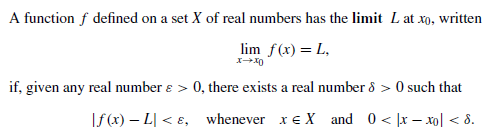
\includegraphics[width=0.75\linewidth]{img01/w01-LimitDef} \end{flushleft}

This definition can be graphically explained in the following figure

\begin{center}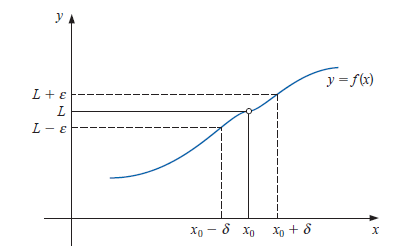
\includegraphics[width=0.75\linewidth]{img01/w01-LimitDefCurve} \end{center}

\hypertarget{continuity}{%
\subsection{Continuity}\label{continuity}}

The continuity of a function is defined based on the concept of limit.

\textbf{Definition}: Let \(f\) be a function defined on a set \(X\) of real numbers and \(x_0 \in X\). Then \(f\) is continuous
at \(x_0\) if
\[
\lim_{x\to x_0}f (x) = f (x_0).
\]
The function \(f\) is continuous on the set \(X\) if it is continuous at each number in \(X\).

\hypertarget{convergence-of-a-sequence}{%
\subsection{Convergence of A Sequence}\label{convergence-of-a-sequence}}

Convergence is one of the fundamental concepts in numerical analysis which is related to the limit of a sequence of real or complex numbers. In numerical analysis, the order of convergence and the rate of convergence of a convergent sequence are quantities that represent how quickly the sequence approaches its limit.

\textbf{Definition}: Let \(\{x_n\}^\infty_{n=1}\) be an infinite sequence of real numbers. This sequence has the \textbf{limit x (converges to x)} if, for any \(\epsilon > 0\) there exists a positive integer \(N(\epsilon)\) such that \(|x_n-x|<\epsilon\), whenever \(n > N(\epsilon)\). The notation
\[
\lim_{n \to\infty}x_n = x, \text{ or } x_n \to x \text{ as } n\to \infty,
\]
means that the sequence \(\{x_n\}^\infty_{n=1}\) converges to \(x\).

\textbf{Definition}: If \(f\) is a function defined on a set \(X\) of real numbers and \(x_0 \in X\), then the following statements are equivalent:

\begin{enumerate}
\def\labelenumi{\alph{enumi}.}
\item
  \(f\) is continuous at \(x_0\);
\item
  If \(\{x_n\}^\infty_{n=1}\) is any sequence in \(X\) converging to \(x_0\), then \(lim_{n\to \infty} f (x_n) = f (x_0)\).
\end{enumerate}

\emph{Remark}: The values of above sequences in \(X\) could be from both sides of \(x_0\).

\url{https://github.com/pengdsci/MAT325/raw/main/w01/img/w01Note1-1-Comvergence.gif}

\hfill\break

\hypertarget{differentiation}{%
\section{Differentiation}\label{differentiation}}

In numerical analysis, many numerical algorithms are based on the assumption that the curve of the underlying function is continuous and \textbf{smooth} over an interval. The smoothness of a curve is characterized by the concept of differentiation.

\hypertarget{definition}{%
\subsection{Definition}\label{definition}}

\textbf{(Average) Rate of Change}: The rate of change of a function \(f(x)\) over interval \([x, x+\Delta x]\) is defined to be
\[
\frac{f(x+\Delta x) - f(x)}{\Delta}
\]

Geometrically, the average rate of change of \(f(x)\) over the interval is the slope of the secant line that passes through the two points on the curve corresponding to the two ending values of the interval.

\textbf{Definition}: Let \(f\) be a function defined in an open interval containing \(x_0\). The function f is differentiable at \(x_0\) if
\[
f^\prime(x_0) = \lim_{x\to x_0}\frac{f (x)-f (x_0)}{x-x_0}
\]

exists. The number \(f(x_0)\) is called the derivative of \(f\) at \(x_0\). A function that has a derivative at each number in a set \(X\) is differentiable on \(X\).

\begin{center}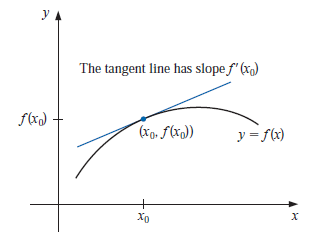
\includegraphics[width=0.75\linewidth]{img01/w01-Derivative} \end{center}

We will assume that you are proficient in using all rules of derivatives. Particularly, the power and chain rules.

\hypertarget{properties}{%
\subsection{Properties}\label{properties}}

Some of the properties and existence theorems will be used in developing numerical algorithms for optimization.

\textbf{Rolle's Theorem}: Suppose \(f \in C[a, b]\) (continuous) and \(f\) is differentiable on \((a, b)\). If \(f (a) = f (b)\), then a number \(c\) in \((a, b)\) exists with \(f(c) = 0\).

\begin{center}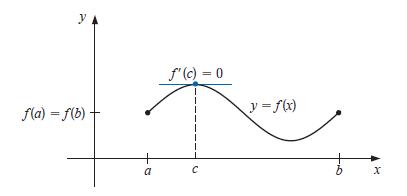
\includegraphics[width=0.75\linewidth]{img01/w01-RolleTheorem} \end{center}

The following mean value theorem is a generalization of Rolle's Theorem.

\textbf{Mean Value Theorem}: If \(f \in C[a, b]\) and f is differentiable on \((a, b)\), then a number \(c\) in \((a, b)\) exists with
\[
\frac{f(b) - f(a)}{b - a}.
\]
We can visualize the mean value theorem in the following figure.

\begin{center}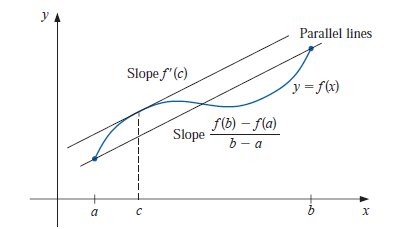
\includegraphics[width=0.75\linewidth]{img01/w01-MeanValue} \end{center}

\textbf{Extreme Value Theorem}: If \(f \in C[a, b]\), then \(c_1, c_2 \in [a, b]\) exist with \(f (c_1) \le f (x) \le f (c_2)\), for all \(x \in [a, b]\). In addition, if \(f\) is differentiable on \((a, b)\), then the numbers \(c_1\) and \(c_2\) occur either at the endpoints of \([a, b]\) or where \(f\) is zero.

\begin{center}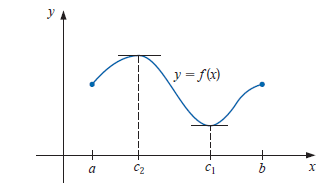
\includegraphics[width=0.75\linewidth]{img01/w01-ExtremeValue} \end{center}

\textbf{Example 1}: Use a computer program to find the absolute minimum and absolute maximum values of
\[
f (x) = 5 \cos (2x) - 2x \sin (2x)
\]
on the intervals \([1, 2]\) and \([0.5, 1]\), respectively.

\textbf{Solution}: We could free online graphing tools such as \emph{WolframAlpha} (\url{https://www.wolframalpha.com/}) to sketch the function. We will use \textbf{R} to plot the function.

\begin{Shaded}
\begin{Highlighting}[]
\NormalTok{x}\OtherTok{=}\FunctionTok{seq}\NormalTok{(}\DecValTok{0}\NormalTok{, }\FloatTok{2.5}\NormalTok{, }\AttributeTok{by =} \FloatTok{0.01}\NormalTok{)}
\NormalTok{y}\OtherTok{=}\DecValTok{5}\SpecialCharTok{*}\FunctionTok{cos}\NormalTok{(}\DecValTok{2}\SpecialCharTok{*}\NormalTok{x) }\SpecialCharTok{{-}} \DecValTok{2}\SpecialCharTok{*}\NormalTok{x}\SpecialCharTok{*}\FunctionTok{sin}\NormalTok{(}\DecValTok{2}\SpecialCharTok{*}\NormalTok{x)}
\FunctionTok{plot}\NormalTok{(x,y, }\AttributeTok{type=}\StringTok{"l"}\NormalTok{, }\AttributeTok{lwd=}\DecValTok{2}\NormalTok{, }\AttributeTok{col=}\StringTok{"navy"}\NormalTok{, }\AttributeTok{bty=}\StringTok{"n"}\NormalTok{)}
\FunctionTok{abline}\NormalTok{(}\AttributeTok{h=}\DecValTok{0}\NormalTok{, }\AttributeTok{lty=}\DecValTok{2}\NormalTok{, }\AttributeTok{col=}\StringTok{"red"}\NormalTok{)}
\FunctionTok{abline}\NormalTok{(}\AttributeTok{v=}\FunctionTok{c}\NormalTok{(}\FloatTok{0.5}\NormalTok{, }\DecValTok{1}\NormalTok{, }\DecValTok{2}\NormalTok{), }\AttributeTok{lty=}\DecValTok{4}\NormalTok{, }\AttributeTok{col=}\StringTok{"skyblue"}\NormalTok{)}
\end{Highlighting}
\end{Shaded}

\begin{center}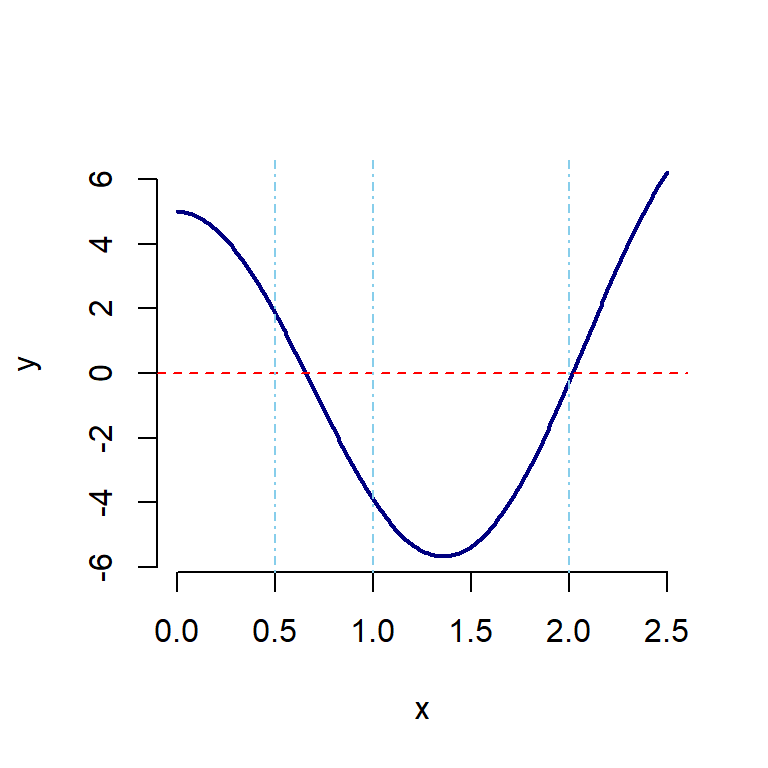
\includegraphics{MAT325EB_files/figure-latex/unnamed-chunk-10-1} \end{center}

(a). We can see from the above figure that, the absolute maximum on \([1, 2]\) is \(f(2) = 5\cos(2\times 2) - 2\times 2 \sin(2\times 2) = -0.2410081\) (see the following code)

\begin{Shaded}
\begin{Highlighting}[]
\DecValTok{5}\SpecialCharTok{*}\FunctionTok{cos}\NormalTok{(}\DecValTok{4}\NormalTok{) }\SpecialCharTok{{-}} \DecValTok{4}\SpecialCharTok{*}\FunctionTok{sin}\NormalTok{(}\DecValTok{4}\NormalTok{)}
\end{Highlighting}
\end{Shaded}

\begin{verbatim}
## [1] -0.24100812
\end{verbatim}

The absolute minimum is the solution to \(f^\prime(x) = 0\). That is, we need to solve equation \(-10\sin(2x) - 2\sin(2x) - 4x\cos(2x) = 0\) that is equivalent to \(\tan(2x) = x/3\). This is a nonlinear equation. There is no closed form of the solution. We will introduce various methods to find the root of this equation. For now, we simply call an R function to find the root.

\begin{Shaded}
\begin{Highlighting}[]
\NormalTok{fn }\OtherTok{=} \ControlFlowTok{function}\NormalTok{(x) }\FunctionTok{tan}\NormalTok{(}\DecValTok{2}\SpecialCharTok{*}\NormalTok{x)}\SpecialCharTok{+}\NormalTok{x}\SpecialCharTok{/}\DecValTok{3}  \CommentTok{\# define the function }
\NormalTok{root }\OtherTok{=} \FunctionTok{nleqslv}\NormalTok{(}\FloatTok{1.5}\NormalTok{, fn)}\SpecialCharTok{$}\NormalTok{x      }\CommentTok{\# the first list $x in the output is the root}
\NormalTok{f.min }\OtherTok{=} \DecValTok{5}\SpecialCharTok{*}\FunctionTok{cos}\NormalTok{(}\DecValTok{2}\SpecialCharTok{*}\NormalTok{root) }\SpecialCharTok{{-}} \DecValTok{2}\SpecialCharTok{*}\NormalTok{root}\SpecialCharTok{*}\FunctionTok{sin}\NormalTok{(}\DecValTok{2}\SpecialCharTok{*}\NormalTok{root)  }\CommentTok{\# finding the absolute minimum}
\FunctionTok{list}\NormalTok{(}\AttributeTok{root =}\NormalTok{ root, }\AttributeTok{abs.min =}\NormalTok{ f.min)}
\end{Highlighting}
\end{Shaded}

\begin{verbatim}
## $root
## [1] 1.3582299
## 
## $abs.min
## [1] -5.6753013
\end{verbatim}

Therefore, the absolute minimum is \(f(1.35823-5.675301) = -5.675301\).

(2). Since the function is strictly decreasing on \([0.5, 1]\), to find the absolute minimum and maximum of the function on \([0.5, 1]\), we simply evaluate the function at \(x = 0.5\) and \(x = 1\) (see the following code).

\begin{Shaded}
\begin{Highlighting}[]
\FunctionTok{list}\NormalTok{(}\AttributeTok{abs.max =} \DecValTok{5}\SpecialCharTok{*}\FunctionTok{cos}\NormalTok{(}\DecValTok{2}\SpecialCharTok{*}\FloatTok{0.5}\NormalTok{) }\SpecialCharTok{{-}} \DecValTok{2}\SpecialCharTok{*}\FloatTok{0.5}\SpecialCharTok{*}\FunctionTok{sin}\NormalTok{(}\DecValTok{2}\SpecialCharTok{*}\FloatTok{0.5}\NormalTok{),}
     \AttributeTok{abs.min =} \DecValTok{5}\SpecialCharTok{*}\FunctionTok{cos}\NormalTok{(}\DecValTok{2}\SpecialCharTok{*}\DecValTok{1}\NormalTok{) }\SpecialCharTok{{-}} \DecValTok{2}\SpecialCharTok{*}\DecValTok{1}\SpecialCharTok{*}\FunctionTok{sin}\NormalTok{(}\DecValTok{2}\SpecialCharTok{*}\DecValTok{1}\NormalTok{))}
\end{Highlighting}
\end{Shaded}

\begin{verbatim}
## $abs.max
## [1] 1.8600405
## 
## $abs.min
## [1] -3.899329
\end{verbatim}

Therefore, the absolute minimum is \(f(1) = -3.899329\) and the absolute maximum \(f(0.5) = 1.860041\).

\textbf{Intermediate Value Theorem}: If \(f \in C[a, b]\) and \(K\) is any number between \(f (a)\) and \(f (b)\), then there exists a number \(c\) in \((a, b)\) for which \(f (c) = K\).

The results in intuitive from the following figure.

\begin{center}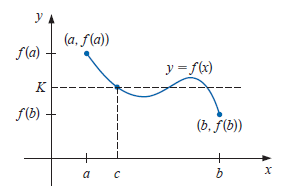
\includegraphics[width=0.75\linewidth]{img01/w01-IntermediateValThm} \end{center}

\hfill\break

\textbf{Example 2}: Show that \(x^5 - 2x^3 + 3x^2 - 1 = 0\) has a solution in the interval \([0, 1]\).

\textbf{Solution}: We want to prove the \emph{existence} of a solution in \([0, 1]\). We first sketch the function in the following.

\begin{Shaded}
\begin{Highlighting}[]
\NormalTok{x }\OtherTok{=} \FunctionTok{seq}\NormalTok{(}\SpecialCharTok{{-}}\FloatTok{0.5}\NormalTok{, }\FloatTok{1.5}\NormalTok{, }\AttributeTok{by =}\FloatTok{0.01}\NormalTok{)}
\NormalTok{y }\OtherTok{=}\NormalTok{ x}\SpecialCharTok{\^{}}\DecValTok{5{-}2}\SpecialCharTok{*}\NormalTok{x}\SpecialCharTok{\^{}}\DecValTok{3} \SpecialCharTok{+} \DecValTok{3}\SpecialCharTok{*}\NormalTok{x}\SpecialCharTok{\^{}}\DecValTok{2{-}1}
\FunctionTok{plot}\NormalTok{(x,y, }\AttributeTok{type=}\StringTok{"l"}\NormalTok{, }\AttributeTok{lwd=}\DecValTok{2}\NormalTok{, }\AttributeTok{col=}\StringTok{"blue"}\NormalTok{, }\AttributeTok{bty=}\StringTok{"n"}\NormalTok{)}
\FunctionTok{abline}\NormalTok{(}\AttributeTok{v=}\FunctionTok{c}\NormalTok{(}\DecValTok{0}\NormalTok{,}\DecValTok{1}\NormalTok{), }\AttributeTok{lty =} \DecValTok{2}\NormalTok{, }\AttributeTok{col =} \StringTok{"purple"}\NormalTok{)}
\FunctionTok{abline}\NormalTok{(}\AttributeTok{h=}\DecValTok{0}\NormalTok{, }\AttributeTok{lty =} \DecValTok{4}\NormalTok{, }\AttributeTok{col=}\StringTok{"darkred"}\NormalTok{)}
\end{Highlighting}
\end{Shaded}

\begin{center}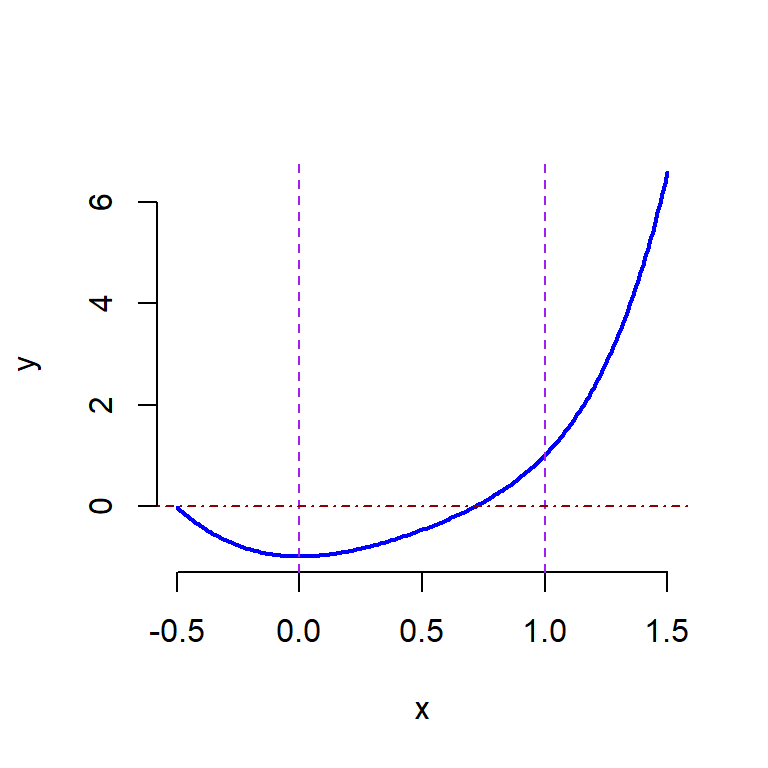
\includegraphics{MAT325EB_files/figure-latex/unnamed-chunk-15-1} \end{center}

After inspecting the curve, choose \(a = 0\) and \(b = 1\) and then use the intermediate value theorem. Note that \(f(0) = -1\) and \(f(1) = 1\). Therefore, \(f(x) = 0\) has a solution in \([0,1]\).

\textbf{Remark}: The intermediate value theorem states that the existence of \emph{at least one solution} in interval \([a, b]\).

\hypertarget{integration}{%
\section{Integration}\label{integration}}

Numerical integration is one of the major topics in numerical analysis. We focus on the definite integral of the single variable function.

\hypertarget{series-vs-sequence}{%
\subsection{Series vs Sequence}\label{series-vs-sequence}}

A \textbf{sequence} is an arrangement of any objects or a set of numbers in a particular order followed by some rule. If \(a_1, a_2, a_3, a_4,\cdots\), denote the terms of a sequence, then \(1,2,3,4, \cdots\) denotes the position of the term. A sequence can be defined based on the number of terms i.e.~either finite sequence or infinite sequence.

If \(a_1, a_2, a_3, a_4,\cdots\) is a sequence, then the corresponding \textbf{series} is given by \(S_n = a_1+a_2+a_3 + \cdots + a_n\) for \(n = 1, 2, \cdots,\). If \(\lim_{n \to \infty} s_n = A\) (\(A\) is finite), then we call series \(s_n\) converges to \(A\).

\hypertarget{definition-of-definite-integral}{%
\subsection{Definition of Definite Integral}\label{definition-of-definite-integral}}

\textbf{Riemann Integral}: The Riemann integral of the function \(f\) on the interval \([a, b]\) is the following limit,
provided it exists:
\[
\int_a^bf(x) dx = \lim_{\max \Delta x_i \to 0} \sum_{i=1}^n f(z_i)\Delta x_i, 
\]
where the numbers \(x_0, x_1, \cdots , x_n\) satisfy \(a = x_0 \le x_1 \le \cdots \le x_n = b\), where \(x_i = x_i - x_{i-1}\), for each \(i = 1, 2, \cdots, n\), and \(z_i\) is arbitrarily chosen in the interval \([x_{i-1}, x_i]\).

\textbf{Remark1}: The above Riemann integral involves two concepts

\begin{enumerate}
\def\labelenumi{\arabic{enumi}.}
\item
  \textbf{Partition of an interval}: \(a = x_0 \le x_1 \le \cdots \le x_n = b\) is also called a partition of interval \([a,b]\).
\item
  \(D_n = \sum_{i=1}^n f(z_i)\Delta x_i\) is so called Darboux sum.
\end{enumerate}

In practice, we take a simple \textbf{equally spaced partition} to evaluate the Riemann integral. To be specific, use the partition such that \(x_i = a + i(b-a)/n\). With this equally-spaced partition, the Riemann integral has the following simple form
\[
\int_a^b f(x) dx = \lim_{n \to \infty}\frac{b-a}{n}\sum_{i=1}^nf(x_i),
\]
The geometric display of the Darboux in the above expression is given below

\begin{center}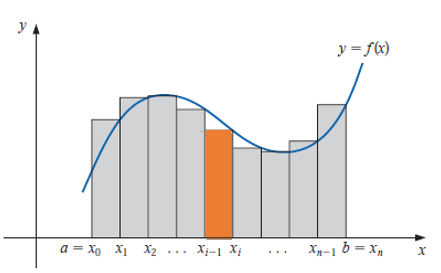
\includegraphics[width=0.75\linewidth]{img01/w01-DarbouxSum} \end{center}

The area of the orange rectangle is the i-th term in the Darboux sum.

The following animated graph shows the process of approximating the integral by the Darboux sum.

\url{https://github.com/pengdsci/MAT325/raw/main/w01/img/w01-GIFRiemannSum.gif}

\hypertarget{taylor-expansion}{%
\subsection{Taylor Expansion}\label{taylor-expansion}}

Since polynomial functions are relatively easier to handle in mathematics. If we want to study the \emph{local} behavior of a complicated function (algebraically), we could use a polynomial to approximate the function locally. The Taylor series is one such polynomial that is used frequently in practice.

\textbf{Taylos's Theroem}: Suppose \(f \in C^n[a,b]\), that \(f^{(n+1)}\) exists on \([a,b]\), and \(x_0 \in [a,b]\). For every \(x \in [a,b]\), there exists a number \(\xi(x)\) between \(x_0\) and \(x\) with

\[
f(x) = P_n(x) + R_n(x),
\]
where
\[
P(x) = f(x_0) + f^\prime(x_0)(x - x_0)+\frac{f^{\prime\prime}(x_0)}{2!}(x-x_0)^2+\cdots+\frac{f^{(n)}(x_0)}{n!}(x-x_0)^n
\]
\[
=\sum_{k=0}^n\frac{f^{(k)}(x_0)}{k!}(x-x_0)^k.
\]
and
\[
R_n(x) = \frac{f^{(n+1)}(\xi(x))}{(n+1)!}(x-x_0)^{n+1}.
\]

Here \(P_n(x)\) is called the \textbf{nth Taylor polynomial} for f about \(x_0\), and \(R_n(x)\) is called the \textbf{remainder term (or truncation error)} associated with \(P_n(x)\).

When \(x_0 = 0\), the Taylor polynomial is called \textbf{Maclaurin polynomial}.

The following animated graph shows the process of Taylor approximation to function \(f(x) =e^{-x}\sin(x)\).

\url{https://github.com/pengdsci/MAT325/blob/main/w01/img/w01Note1-1-TaylorExansion02.gif}

\hfill\break

\textbf{Example}: Let \(f (x) = cos x\) and \(x_0 = 0\). Determine the second Taylor polynomial for \(f\) about \(x_0\).

\textbf{Solution}: We use the Taylor theorem to expand \(cos(x)\) up two 2nd order
\[
cos(x) = f(0) + f^\prime(0)x+\frac{f^{\prime\prime}(0)}{2!}x^2+\frac{f^{(\xi(x))}(0)}{3!}x^3
\]
\[
=1 - \frac{1}{2}x^2+\frac{1}{6}x^3\sin[\xi(x)].
\]
where \(\xi(x)\) is in \([0, x]\). The following figure shows the approximation.

\begin{center}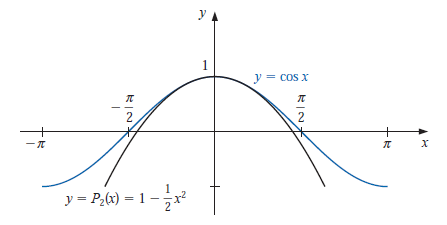
\includegraphics[width=0.75\linewidth]{img01/w01-MacclaurinExpansion} \end{center}

\hypertarget{scientific-computing-with-r}{%
\chapter{Scientific Computing with R}\label{scientific-computing-with-r}}

R was initially created by group of statisticians for data analysis (for free). In the past decade, many people from other disciplines contributed to the continuous development of this program. It is among the top programming language in data science and machine learning and widely used to perform a variety of non-statistical tasks, including data processing, information visualization, data mining, and scientific computing, etc.

During the semester, I will write series of short notes on R to implement numerical algorithms to be covered in the course. I will also write one or two lab notes to cover optimization problems in machine learning and data science.

The following three books focus on using R for scientific computing. You can find one of them as a reference when you make programs for this class.

\begin{enumerate}
\def\labelenumi{\arabic{enumi}.}
\item
  \textbf{Introduction to scientific programming and simulation using R}. This book can be found from internet.
\item
  \textbf{Mastering Scientific Computing with R}. WCU library has this eBook. You can access this book using the following link. \url{https://ebookcentral.proquest.com/lib/wcupa/detail.action?pq-origsite=primo\&docID=1936749}
\item
  \textbf{Using R Numerical Analysis in Science and Engineering}. You can also find this from internet.
\end{enumerate}

For those who programmed in MATLAB, you can check the following page to see the back-to-back syntax comparison between R and MATLAB \url{https://mathesaurus.sourceforge.net/octave-r.html}.

\textbf{\color{red} R is case sensitive!}.

\hypertarget{vectors-and-matrices}{%
\section{Vectors and Matrices}\label{vectors-and-matrices}}

Vectors and matrices are two major R objects that will be used frequently in numerical analysis. This section outlines the definition and utilization of vectors and matrices.

\hypertarget{vectors}{%
\subsection{Vectors}\label{vectors}}

A vector is a collection of \emph{like} elements without dimensions. The vector element or elements must be of the same types of data (either \textbf{character}, \textbf{numeric}, or \textbf{logical}).

\hypertarget{definition-1}{%
\subsubsection{Definition}\label{definition-1}}

An R vector defined by a built-in R function \texttt{c()} (\textbf{c} stands for concatenate). The following are examples of basic types of vectors.

\begin{Shaded}
\begin{Highlighting}[]
\NormalTok{intVec }\OtherTok{\textless{}{-}} \FunctionTok{c}\NormalTok{(}\DecValTok{1}\NormalTok{,}\DecValTok{3}\NormalTok{,}\DecValTok{6}\NormalTok{,}\DecValTok{7}\NormalTok{)                  }\CommentTok{\# vector of integers}
\NormalTok{charVec }\OtherTok{=} \FunctionTok{c}\NormalTok{(}\StringTok{\textquotesingle{}One\textquotesingle{}}\NormalTok{,}\StringTok{\textquotesingle{}Two\textquotesingle{}}\NormalTok{,}\StringTok{\textquotesingle{}Three\textquotesingle{}}\NormalTok{)      }\CommentTok{\# vector of characters, string vector}
\NormalTok{logiVec }\OtherTok{=} \FunctionTok{c}\NormalTok{(}\ConstantTok{FALSE}\NormalTok{, }\ConstantTok{TRUE}\NormalTok{)              }\CommentTok{\# logical vectors}
\NormalTok{single.Val.Vec }\OtherTok{=} \FunctionTok{c}\NormalTok{(}\StringTok{"convergent"}\NormalTok{)      }\CommentTok{\# single element character vector}
\NormalTok{emptyVec }\OtherTok{=} \ConstantTok{NULL}                       \CommentTok{\# empty vector / null vector }
\DocumentationTok{\#\# }
\NormalTok{intVec                                }\CommentTok{\# type the of the name of intVec}
\end{Highlighting}
\end{Shaded}

\begin{verbatim}
## [1] 1 3 6 7
\end{verbatim}

\hypertarget{use-of-vector-index}{%
\subsubsection{Use of Vector Index}\label{use-of-vector-index}}

One can access elements in a vector through index using square bracket \texttt{{[}idx{]}}. Similar to MATLAB, \textbf{R index starts from 1}!

\begin{Shaded}
\begin{Highlighting}[]
\NormalTok{exampleVec }\OtherTok{=} \FunctionTok{c}\NormalTok{(}\DecValTok{1}\NormalTok{, }\DecValTok{2}\NormalTok{, }\DecValTok{3}\NormalTok{, }\DecValTok{2}\NormalTok{, }\DecValTok{7}\NormalTok{, }\DecValTok{9}\NormalTok{, }\DecValTok{11}\NormalTok{, }\DecValTok{15}\NormalTok{, }\DecValTok{7}\NormalTok{, }\DecValTok{2}\NormalTok{)  }\CommentTok{\# use this vector as an example}
\DocumentationTok{\#\#\#}
\NormalTok{exampleVec[}\DecValTok{7}\NormalTok{]            }\CommentTok{\# extract the 7th element in the vector}
\end{Highlighting}
\end{Shaded}

\begin{verbatim}
## [1] 11
\end{verbatim}

\begin{Shaded}
\begin{Highlighting}[]
\NormalTok{exampleVec[}\FunctionTok{c}\NormalTok{(}\DecValTok{1}\NormalTok{,}\DecValTok{2}\NormalTok{,}\DecValTok{3}\NormalTok{)]     }\CommentTok{\# extract the first three elements, c(1,2,3) is the vector of indexes}
\end{Highlighting}
\end{Shaded}

\begin{verbatim}
## [1] 1 2 3
\end{verbatim}

\begin{Shaded}
\begin{Highlighting}[]
\NormalTok{exampleVec[}\SpecialCharTok{{-}}\DecValTok{7}\NormalTok{]           }\CommentTok{\# drop the 7th element from the vector}
\end{Highlighting}
\end{Shaded}

\begin{verbatim}
## [1]  1  2  3  2  7  9 15  7  2
\end{verbatim}

\begin{Shaded}
\begin{Highlighting}[]
\NormalTok{exampleVec[}\SpecialCharTok{{-}}\FunctionTok{c}\NormalTok{(}\DecValTok{1}\NormalTok{,}\DecValTok{2}\NormalTok{,}\DecValTok{3}\NormalTok{)]    }\CommentTok{\# drop the first three elements}
\end{Highlighting}
\end{Shaded}

\begin{verbatim}
## [1]  2  7  9 11 15  7  2
\end{verbatim}

\begin{Shaded}
\begin{Highlighting}[]
\NormalTok{duplVec }\OtherTok{=}\NormalTok{ exampleVec     }\CommentTok{\# duplicate an existing vector and rename it}
\DocumentationTok{\#\# The following code replaces elements with NEW elements}
\NormalTok{duplVec[}\FunctionTok{c}\NormalTok{(}\DecValTok{9}\NormalTok{,}\DecValTok{10}\NormalTok{)] }\OtherTok{=} \FunctionTok{c}\NormalTok{(}\DecValTok{99}\NormalTok{,}\DecValTok{100}\NormalTok{)   }\CommentTok{\# replace elements 7, 4 with 99 and 100 respectively.}
\NormalTok{duplVec                  }\CommentTok{\# display the modified vector}
\end{Highlighting}
\end{Shaded}

\begin{verbatim}
##  [1]   1   2   3   2   7   9  11  15  99 100
\end{verbatim}

\hypertarget{operations-between-vectors}{%
\subsubsection{Operations Between Vectors}\label{operations-between-vectors}}

The following examples show the operations commonly used in error analysis.

\begin{Shaded}
\begin{Highlighting}[]
\NormalTok{A }\OtherTok{=} \FunctionTok{c}\NormalTok{(}\DecValTok{5}\NormalTok{, }\DecValTok{2}\NormalTok{, }\DecValTok{3}\NormalTok{, }\DecValTok{7}\NormalTok{, }\DecValTok{5}\NormalTok{, }\DecValTok{1}\NormalTok{, }\DecValTok{9}\NormalTok{)}
\NormalTok{B }\OtherTok{=} \FunctionTok{c}\NormalTok{(}\DecValTok{3}\NormalTok{, }\DecValTok{2}\NormalTok{, }\DecValTok{4}\NormalTok{, }\DecValTok{8}\NormalTok{, }\DecValTok{2}\NormalTok{, }\DecValTok{7}\NormalTok{)}
\DocumentationTok{\#\# next we define different new vectors using A and B}
\NormalTok{new01 }\OtherTok{=} \FunctionTok{c}\NormalTok{(A,B)    }\CommentTok{\# concatenate A and B}
\NormalTok{new01             }\CommentTok{\# display new01}
\end{Highlighting}
\end{Shaded}

\begin{verbatim}
##  [1] 5 2 3 7 5 1 9 3 2 4 8 2 7
\end{verbatim}

\begin{Shaded}
\begin{Highlighting}[]
\NormalTok{new02 }\OtherTok{=}\NormalTok{ A}\DecValTok{{-}5}       \CommentTok{\# subtract 5 from individual element in A }
\NormalTok{new02}
\end{Highlighting}
\end{Shaded}

\begin{verbatim}
## [1]  0 -3 -2  2  0 -4  4
\end{verbatim}

\begin{Shaded}
\begin{Highlighting}[]
\NormalTok{new03 }\OtherTok{=}\NormalTok{ A}\SpecialCharTok{\^{}}\DecValTok{2}       \CommentTok{\# square each individual element in A}
\NormalTok{new03}
\end{Highlighting}
\end{Shaded}

\begin{verbatim}
## [1] 25  4  9 49 25  1 81
\end{verbatim}

\begin{Shaded}
\begin{Highlighting}[]
\NormalTok{new04 }\OtherTok{=} \DecValTok{2}\SpecialCharTok{*}\NormalTok{A       }\CommentTok{\# multiply each element of A by 2}
\NormalTok{new04}
\end{Highlighting}
\end{Shaded}

\begin{verbatim}
## [1] 10  4  6 14 10  2 18
\end{verbatim}

\hypertarget{shortcuts-for-defining-vectors}{%
\subsubsection{Shortcuts for Defining Vectors}\label{shortcuts-for-defining-vectors}}

There are shortcuts to define patterned vectors (sequence). The following are few examples.

\begin{Shaded}
\begin{Highlighting}[]
\NormalTok{seq.vec }\OtherTok{=} \FunctionTok{seq}\NormalTok{(}\DecValTok{1}\NormalTok{, }\DecValTok{100}\NormalTok{, }\AttributeTok{by =} \DecValTok{2}\NormalTok{)       }\CommentTok{\# This defines a sequence: 1, 3, 5, 7, ..., 99. by = jump}
\NormalTok{seq.vec}
\end{Highlighting}
\end{Shaded}

\begin{verbatim}
##  [1]  1  3  5  7  9 11 13 15 17 19 21 23 25 27 29 31 33 35 37 39 41 43 45 47 49 51 53 55 57 59 61 63 65 67 69 71 73
## [38] 75 77 79 81 83 85 87 89 91 93 95 97 99
\end{verbatim}

\begin{Shaded}
\begin{Highlighting}[]
\NormalTok{seq.vec01 }\OtherTok{=} \FunctionTok{seq}\NormalTok{(}\DecValTok{1}\NormalTok{, }\DecValTok{99}\NormalTok{, }\AttributeTok{length =} \DecValTok{5}\NormalTok{)  }\CommentTok{\# This defines a sequence with 5 numbers that are equally spaced between 1 and 99.}
\NormalTok{seq.vec01}
\end{Highlighting}
\end{Shaded}

\begin{verbatim}
## [1]  1.0 25.5 50.0 74.5 99.0
\end{verbatim}

\begin{Shaded}
\begin{Highlighting}[]
\NormalTok{seq.vec02 }\OtherTok{=} \FunctionTok{rep}\NormalTok{(}\DecValTok{1}\NormalTok{, }\DecValTok{100}\NormalTok{)             }\CommentTok{\# This defines a sequence with 100 1s.}
\NormalTok{seq.vec02}
\end{Highlighting}
\end{Shaded}

\begin{verbatim}
##   [1] 1 1 1 1 1 1 1 1 1 1 1 1 1 1 1 1 1 1 1 1 1 1 1 1 1 1 1 1 1 1 1 1 1 1 1 1 1 1 1 1 1 1 1 1 1 1 1 1 1 1 1 1 1 1 1
##  [56] 1 1 1 1 1 1 1 1 1 1 1 1 1 1 1 1 1 1 1 1 1 1 1 1 1 1 1 1 1 1 1 1 1 1 1 1 1 1 1 1 1 1 1 1 1
\end{verbatim}

\begin{Shaded}
\begin{Highlighting}[]
\NormalTok{seq.vec03 }\OtherTok{=} \DecValTok{3}\SpecialCharTok{:}\DecValTok{10}                    \CommentTok{\# This sequence: 3,4,5,6,7,8,9,10.}
\NormalTok{seq.vec03}
\end{Highlighting}
\end{Shaded}

\begin{verbatim}
## [1]  3  4  5  6  7  8  9 10
\end{verbatim}

\begin{Shaded}
\begin{Highlighting}[]
\NormalTok{seq.vec04 }\OtherTok{=}\NormalTok{ letters                 }\CommentTok{\# letters is a built{-}in vector of all lower case letters    }
\NormalTok{seq.vec04}
\end{Highlighting}
\end{Shaded}

\begin{verbatim}
##  [1] "a" "b" "c" "d" "e" "f" "g" "h" "i" "j" "k" "l" "m" "n" "o" "p" "q" "r" "s" "t" "u" "v" "w" "x" "y" "z"
\end{verbatim}

\begin{Shaded}
\begin{Highlighting}[]
\NormalTok{seq.vec05 }\OtherTok{=}\NormalTok{ LETTERS                 }\CommentTok{\# LETTERS is a built{-}in vector of all uppercase letters}
\NormalTok{seq.vec05}
\end{Highlighting}
\end{Shaded}

\begin{verbatim}
##  [1] "A" "B" "C" "D" "E" "F" "G" "H" "I" "J" "K" "L" "M" "N" "O" "P" "Q" "R" "S" "T" "U" "V" "W" "X" "Y" "Z"
\end{verbatim}

\begin{Shaded}
\begin{Highlighting}[]
\NormalTok{LETTERS[}\DecValTok{1}\SpecialCharTok{:}\DecValTok{7}\NormalTok{]                        }\CommentTok{\# first 7 uppercase letters.}
\end{Highlighting}
\end{Shaded}

\begin{verbatim}
## [1] "A" "B" "C" "D" "E" "F" "G"
\end{verbatim}

\hypertarget{matrices}{%
\subsection{Matrices}\label{matrices}}

R matrices are two dimensional table indexed by two subscripts using \([i,j]\), where \(i\) = index of row of the matrix and \(j\) = index of the column of the matrix. On can access the matrix using index \([i,j]\). The following are some examples of matrices

\begin{Shaded}
\begin{Highlighting}[]
\NormalTok{vec0 }\OtherTok{=} \DecValTok{1}\SpecialCharTok{:}\DecValTok{36}
\NormalTok{m01 }\OtherTok{=} \FunctionTok{matrix}\NormalTok{(vec0, }\AttributeTok{ncol =} \DecValTok{9}\NormalTok{, }\AttributeTok{byrow =} \ConstantTok{TRUE}\NormalTok{)   }\CommentTok{\# this defines a 4x9 matrix, the cells were filled from vec0 by rows}
\NormalTok{m01 }
\end{Highlighting}
\end{Shaded}

\begin{verbatim}
##      [,1] [,2] [,3] [,4] [,5] [,6] [,7] [,8] [,9]
## [1,]    1    2    3    4    5    6    7    8    9
## [2,]   10   11   12   13   14   15   16   17   18
## [3,]   19   20   21   22   23   24   25   26   27
## [4,]   28   29   30   31   32   33   34   35   36
\end{verbatim}

\begin{Shaded}
\begin{Highlighting}[]
\NormalTok{m02 }\OtherTok{=} \FunctionTok{matrix}\NormalTok{(vec0, }\AttributeTok{nrow =} \DecValTok{6}\NormalTok{, }\AttributeTok{byrow =} \ConstantTok{FALSE}\NormalTok{)  }\CommentTok{\# this defines a 6x6 square matrix, cells were filled from vec0 by column}
\NormalTok{m02}
\end{Highlighting}
\end{Shaded}

\begin{verbatim}
##      [,1] [,2] [,3] [,4] [,5] [,6]
## [1,]    1    7   13   19   25   31
## [2,]    2    8   14   20   26   32
## [3,]    3    9   15   21   27   33
## [4,]    4   10   16   22   28   34
## [5,]    5   11   17   23   29   35
## [6,]    6   12   18   24   30   36
\end{verbatim}

\begin{Shaded}
\begin{Highlighting}[]
\NormalTok{m03 }\OtherTok{=} \FunctionTok{matrix}\NormalTok{(}\AttributeTok{ncol =} \DecValTok{5}\NormalTok{, }\AttributeTok{nrow =} \DecValTok{6}\NormalTok{)       }\CommentTok{\# this defined a 5x6 empty matrix}
\NormalTok{m03}
\end{Highlighting}
\end{Shaded}

\begin{verbatim}
##      [,1] [,2] [,3] [,4] [,5]
## [1,]   NA   NA   NA   NA   NA
## [2,]   NA   NA   NA   NA   NA
## [3,]   NA   NA   NA   NA   NA
## [4,]   NA   NA   NA   NA   NA
## [5,]   NA   NA   NA   NA   NA
## [6,]   NA   NA   NA   NA   NA
\end{verbatim}

\begin{Shaded}
\begin{Highlighting}[]
\NormalTok{m03[}\DecValTok{4}\NormalTok{,}\DecValTok{5}\NormalTok{] }\OtherTok{=} \DecValTok{99}                          \CommentTok{\# replace the element in row 4 and column 5 with 99.}
\NormalTok{m03}
\end{Highlighting}
\end{Shaded}

\begin{verbatim}
##      [,1] [,2] [,3] [,4] [,5]
## [1,]   NA   NA   NA   NA   NA
## [2,]   NA   NA   NA   NA   NA
## [3,]   NA   NA   NA   NA   NA
## [4,]   NA   NA   NA   NA   99
## [5,]   NA   NA   NA   NA   NA
## [6,]   NA   NA   NA   NA   NA
\end{verbatim}

\hfill\break

\hypertarget{built-in-mathematical-functions-and-operators}{%
\section{Built-in Mathematical Functions and Operators}\label{built-in-mathematical-functions-and-operators}}

R has built in most of the commonly used mathematical functions and important scalars. The following is a partial list.

\hypertarget{arithmetic-operators}{%
\subsection{Arithmetic Operators}\label{arithmetic-operators}}

\texttt{+} -- addition

\texttt{–} -- subtraction

\texttt{*} -- multiplication

\texttt{/} -- division

\texttt{\^{}} -- raise to the power of

\hypertarget{basic-mathematical-functions}{%
\subsection{Basic Mathematical Functions}\label{basic-mathematical-functions}}

\texttt{abs()} - absolute value

\texttt{sqrt()} - square root

\texttt{round()} - rounding function

\texttt{ceiling()} - rounding up

\texttt{floor()} - rounding down

\texttt{sign()} - sign of a number

\texttt{exp()} - natural base exponential function

\texttt{log()} - natural base logarithmic function

\texttt{log10()} - base 10 logarithmic function

\hypertarget{trigonometry}{%
\subsection{Trigonometry}\label{trigonometry}}

\texttt{sin()} -- sine

\texttt{cos()} -- cosine

\texttt{tan()} -- tangent

\texttt{asin()} -- sine inverse

\texttt{acos()} -- cosine inverse

\texttt{atan()} -- tangent inverse

\hypertarget{linear-algebra}{%
\subsection{Linear Algebra}\label{linear-algebra}}

\texttt{+} -- element-wise addition

\texttt{–} -- element-wise subtraction

\texttt{*} -- element-wise multiplication

\texttt{/} -- element-wise division

\texttt{\%*\%} -- matrix multiplication

\texttt{t()} -- transpose

\texttt{eigen()} -- eigenvalues and eigenvectors

\texttt{solve()} -- inverse of matrix

\texttt{rbind()} -- combines vectors of observations horizontally into matrix class

\texttt{cbind()} -- combines vectors of observations vertically into matrix class

\hfill\break

\hypertarget{graphic-functions-in-base-r}{%
\section{Graphic Functions in Base R}\label{graphic-functions-in-base-r}}

Base R graphical system contains a set of \textbf{high-level plotting functions} such as \texttt{plot()}, \texttt{hist()}, \texttt{barplot()}, etc. and also a set of \textbf{low-level functions} that are used jointly with the high-level plotting functions such as \texttt{points()}, \texttt{lines()}, \texttt{text()}, \texttt{segments()}, etc. to make a flexible graphical system.

Next we use a simple example to illustrate the basic graphic functions. We draw the curves of two functions \(f_1(x) = \sin(x)\) and \(f_2(x) = \cos(x)\) over interval \([-2\pi, 2\pi]\).

\begin{Shaded}
\begin{Highlighting}[]
\NormalTok{x }\OtherTok{=} \FunctionTok{seq}\NormalTok{(}\SpecialCharTok{{-}}\DecValTok{2}\SpecialCharTok{*}\NormalTok{pi, }\DecValTok{2}\SpecialCharTok{*}\NormalTok{pi, }\AttributeTok{length =} \DecValTok{200}\NormalTok{)  }\CommentTok{\# define a sequence of numbers on the interval}
\NormalTok{f1 }\OtherTok{=} \FunctionTok{sin}\NormalTok{(x)                         }\CommentTok{\# evaluate f1 = sin(x) at these values}
\NormalTok{f2 }\OtherTok{=} \FunctionTok{cos}\NormalTok{(x)                         }\CommentTok{\# evaluate f2 = cos(x) at these values}
\DocumentationTok{\#\#}
\FunctionTok{plot}\NormalTok{(x, f1,                         }\CommentTok{\# x{-} and y{-} coordinates}
        \AttributeTok{type =} \StringTok{"l"}\NormalTok{,                 }\CommentTok{\# lower case l in the quote means line. The default option is point. "b" = both line and point.}
        \AttributeTok{xlab =} \StringTok{"X Value"}\NormalTok{,           }\CommentTok{\# label of x{-}axis, if not specified, the name of x vector will be used}
        \AttributeTok{ylab =} \StringTok{"Y value"}\NormalTok{, }
        \AttributeTok{ylim =} \FunctionTok{c}\NormalTok{(}\SpecialCharTok{{-}}\FloatTok{1.5}\NormalTok{, }\FloatTok{2.0}\NormalTok{),        }\CommentTok{\# the limits of y{-}axis, must be a vector of two values. The default limits are min and max of f1}
        \AttributeTok{xlim =} \FunctionTok{c}\NormalTok{(}\SpecialCharTok{{-}}\DecValTok{2}\SpecialCharTok{*}\NormalTok{pi, }\DecValTok{2}\SpecialCharTok{*}\NormalTok{pi),      }\CommentTok{\# the limits of x{-}axis, if it is not provided, the min and max values of x will be used.}
        \AttributeTok{col =} \StringTok{"red"}\NormalTok{,                }\CommentTok{\# select a color for the line}
        \AttributeTok{lty =} \DecValTok{1}\NormalTok{,                    }\CommentTok{\# line type. 1 = solid, 2 = dash, ....}
        \AttributeTok{cex =} \FloatTok{1.2}\NormalTok{,                  }\CommentTok{\# size, default = 1}
        \AttributeTok{main =} \StringTok{"The curves of sin(x) and cos(x)"}\NormalTok{,   }\CommentTok{\# the title of the plot.}
        \AttributeTok{bty =} \StringTok{"n"}                   \CommentTok{\# remove the outbox on the plot. The default plot has an outer box.}
\NormalTok{     )}
\FunctionTok{abline}\NormalTok{(}\AttributeTok{h =} \DecValTok{0}\NormalTok{, }\AttributeTok{lty =} \DecValTok{4}\NormalTok{, }\AttributeTok{col =} \StringTok{"darkgreen"}\NormalTok{)                       }\CommentTok{\# add a horizontal line at y = 0}
\FunctionTok{lines}\NormalTok{(x, f2, }\AttributeTok{lty =} \DecValTok{2}\NormalTok{, }\AttributeTok{lwd =} \DecValTok{2}\NormalTok{, }\AttributeTok{col =} \StringTok{"blue"}\NormalTok{)                    }\CommentTok{\# cos(x) curve to the existing plot. Caution: use lines(), not plot().}
\DocumentationTok{\#\# add a few special points on both curves}
\NormalTok{pt.x }\OtherTok{=} \FunctionTok{seq}\NormalTok{(}\SpecialCharTok{{-}}\DecValTok{2}\SpecialCharTok{*}\NormalTok{pi, }\DecValTok{2}\SpecialCharTok{*}\NormalTok{pi, }\AttributeTok{length =} \DecValTok{9}\NormalTok{)                             }\CommentTok{\# select 9 x{-}coordinates to make 9 points}
\NormalTok{pt.y1 }\OtherTok{=} \FunctionTok{sin}\NormalTok{(pt.x)                                               }\CommentTok{\# }
\NormalTok{pt.y2 }\OtherTok{=} \FunctionTok{cos}\NormalTok{(pt.x)}
\DocumentationTok{\#\# Adding points to the two curves}
\FunctionTok{points}\NormalTok{(pt.x, pt.y1,                    }\CommentTok{\# add points to f1 = sin(x)}
         \AttributeTok{pch =} \DecValTok{16}\NormalTok{,                     }\CommentTok{\# point types, there 20+ types of points in R}
         \AttributeTok{col =} \StringTok{"red"}\NormalTok{,}
         \AttributeTok{cex =} \FloatTok{1.5}\NormalTok{)                    }\CommentTok{\# size of the points, default cex = 1}
\FunctionTok{points}\NormalTok{(pt.x, pt.y2, }\AttributeTok{pch =} \DecValTok{21}\NormalTok{, }\AttributeTok{col =} \StringTok{"blue"}\NormalTok{, }\AttributeTok{cex =} \FloatTok{1.5}\NormalTok{)}
\DocumentationTok{\#\# adding legends}
\FunctionTok{legend}\NormalTok{(}\StringTok{"top"}\NormalTok{,      }\CommentTok{\# location of the legend, other locations: "bottom", "topleft", "topright" bottomleft", "bottomright", providing}
                   \CommentTok{\# the coordinates of the location to place the legend.}
              \FunctionTok{c}\NormalTok{(}\StringTok{"sin(x)"}\NormalTok{, }\StringTok{"cos(x)"}\NormalTok{),         }\CommentTok{\# label of the corresponding curves}
              \AttributeTok{pch =} \FunctionTok{c}\NormalTok{(}\DecValTok{16}\NormalTok{, }\DecValTok{21}\NormalTok{),               }\CommentTok{\# the corresponding point type}
              \AttributeTok{col =} \FunctionTok{c}\NormalTok{(}\StringTok{"red"}\NormalTok{, }\StringTok{"blue"}\NormalTok{),        }\CommentTok{\# corresponding color}
              \AttributeTok{lty =} \FunctionTok{c}\NormalTok{(}\DecValTok{1}\NormalTok{, }\DecValTok{2}\NormalTok{),                 }\CommentTok{\# corresponding line type}
              \AttributeTok{lwd =} \FunctionTok{c}\NormalTok{(}\DecValTok{2}\NormalTok{,}\DecValTok{2}\NormalTok{),                  }\CommentTok{\# corresponding line width}
              \AttributeTok{bty =} \StringTok{"n"}\NormalTok{)                     }\CommentTok{\# no box placed around the legend}
\end{Highlighting}
\end{Shaded}

\begin{center}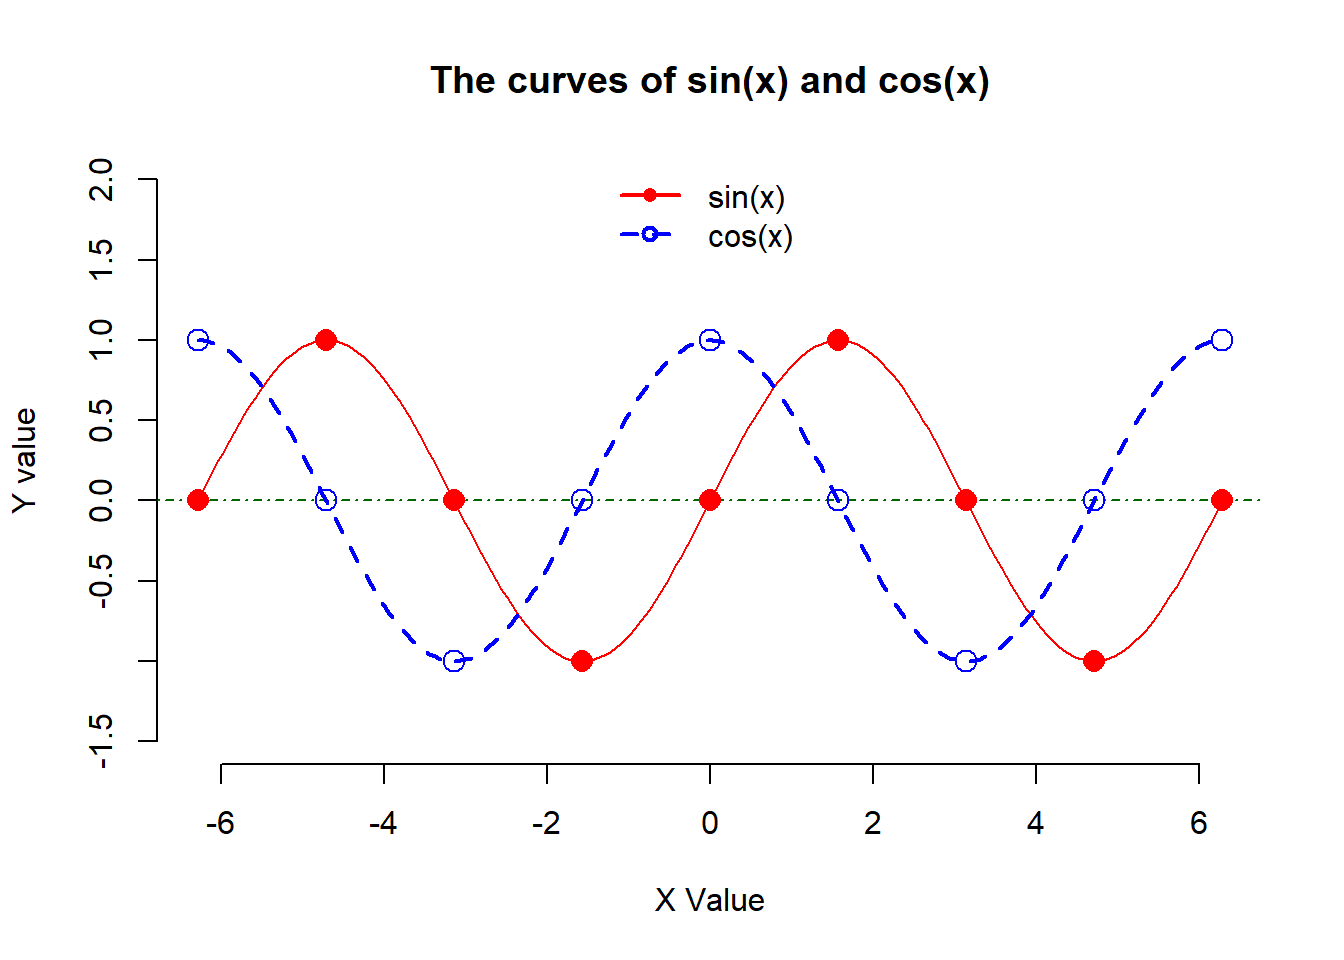
\includegraphics{MAT325EB_files/figure-latex/unnamed-chunk-25-1} \end{center}

\hypertarget{rounding-and-related-functions}{%
\section{Rounding and Related Functions}\label{rounding-and-related-functions}}

There are several R functions we can use to handle decimals and manage significant digits in numerical analysis. A list of a few such functions in the base R.

\hypertarget{round}{%
\subsection{round()}\label{round}}

\texttt{round(number,digits)} rounds the number to the number of digits provided. Here is an example of the round function in action.

\begin{Shaded}
\begin{Highlighting}[]
\FunctionTok{round}\NormalTok{(}\FloatTok{1234.56789}\NormalTok{,}\DecValTok{3}\NormalTok{)    }\CommentTok{\# keep three decimal places}
\end{Highlighting}
\end{Shaded}

\begin{verbatim}
## [1] 1234.568
\end{verbatim}

\begin{Shaded}
\begin{Highlighting}[]
\FunctionTok{round}\NormalTok{(}\FloatTok{1234.56789}\NormalTok{,}\DecValTok{5}\NormalTok{)    }\CommentTok{\# R only displays 7 digits by default}
\end{Highlighting}
\end{Shaded}

\begin{verbatim}
## [1] 1234.5679
\end{verbatim}

\begin{Shaded}
\begin{Highlighting}[]
\FunctionTok{round}\NormalTok{(}\FloatTok{1234.56789}\NormalTok{,}\DecValTok{0}\NormalTok{)    }\CommentTok{\# keep no decimal place}
\end{Highlighting}
\end{Shaded}

\begin{verbatim}
## [1] 1235
\end{verbatim}

\begin{Shaded}
\begin{Highlighting}[]
\FunctionTok{round}\NormalTok{(}\FloatTok{1234.56789}\NormalTok{,}\SpecialCharTok{{-}}\DecValTok{3}\NormalTok{)   }\CommentTok{\# set three digits before decimal points to zeros}
\end{Highlighting}
\end{Shaded}

\begin{verbatim}
## [1] 1000
\end{verbatim}

\begin{Shaded}
\begin{Highlighting}[]
\FunctionTok{round}\NormalTok{(}\FloatTok{1234.56789}\NormalTok{,}\SpecialCharTok{{-}}\DecValTok{5}\NormalTok{)}
\end{Highlighting}
\end{Shaded}

\begin{verbatim}
## [1] 0
\end{verbatim}

\hypertarget{controlling-number-of-displayed-digits}{%
\subsection{Controlling Number of Displayed Digits}\label{controlling-number-of-displayed-digits}}

There are different ways to change the number of displayed digits. We can change the default \texttt{option(digits\ =\ 7)} to \texttt{option(digits\ =\ 10)} to display 10 digits (Caution: this is a global option!).

\begin{Shaded}
\begin{Highlighting}[]
\FunctionTok{options}\NormalTok{(}\AttributeTok{digits =} \DecValTok{10}\NormalTok{)}
\FunctionTok{round}\NormalTok{(}\FloatTok{1234.56789}\NormalTok{,}\DecValTok{3}\NormalTok{)    }\CommentTok{\# keep three decimal places}
\end{Highlighting}
\end{Shaded}

\begin{verbatim}
## [1] 1234.568
\end{verbatim}

\begin{Shaded}
\begin{Highlighting}[]
\FunctionTok{round}\NormalTok{(}\FloatTok{1234.56789}\NormalTok{,}\DecValTok{5}\NormalTok{)    }\CommentTok{\# R only displays 7 digits by default}
\end{Highlighting}
\end{Shaded}

\begin{verbatim}
## [1] 1234.56789
\end{verbatim}

\begin{Shaded}
\begin{Highlighting}[]
\FunctionTok{round}\NormalTok{(}\FloatTok{1234.56789}\NormalTok{,}\DecValTok{6}\NormalTok{)    }\CommentTok{\# R only displays 7 digits by default}
\end{Highlighting}
\end{Shaded}

\begin{verbatim}
## [1] 1234.56789
\end{verbatim}

The c-style formatting function can also be used to display the desired number of digits.

\begin{Shaded}
\begin{Highlighting}[]
\FunctionTok{sqrt}\NormalTok{(}\DecValTok{2}\NormalTok{)                     }\CommentTok{\# this will display 10 digits. why?}
\end{Highlighting}
\end{Shaded}

\begin{verbatim}
## [1] 1.414213562
\end{verbatim}

\begin{Shaded}
\begin{Highlighting}[]
\FunctionTok{sprintf}\NormalTok{(}\StringTok{"\%.20f"}\NormalTok{, }\FunctionTok{sqrt}\NormalTok{(}\DecValTok{2}\NormalTok{))   }\CommentTok{\# Note this displays a string value}
\end{Highlighting}
\end{Shaded}

\begin{verbatim}
## [1] "1.41421356237309514547"
\end{verbatim}

\begin{Shaded}
\begin{Highlighting}[]
\FunctionTok{options}\NormalTok{(}\AttributeTok{digits =} \DecValTok{20}\NormalTok{)        }\CommentTok{\# change options to display 20 digits}
\FunctionTok{sqrt}\NormalTok{(}\DecValTok{2}\NormalTok{)}
\end{Highlighting}
\end{Shaded}

\begin{verbatim}
## [1] 1.4142135623730951455
\end{verbatim}

\begin{Shaded}
\begin{Highlighting}[]
\FunctionTok{options}\NormalTok{(}\AttributeTok{digits =} \DecValTok{7}\NormalTok{)         }\CommentTok{\# change the options back to the default}
\end{Highlighting}
\end{Shaded}

\hypertarget{signif}{%
\subsection{\texorpdfstring{\texttt{Signif()}}{Signif()}}\label{signif}}

\texttt{Signif()} is an R \textbf{rounding function} with the format of \texttt{signif(number,digits)} and it \textbf{rounds} the number to the number of digits provided.

\begin{Shaded}
\begin{Highlighting}[]
\FunctionTok{signif}\NormalTok{(}\FloatTok{1234.566789}\NormalTok{,}\DecValTok{4}\NormalTok{)}
\end{Highlighting}
\end{Shaded}

\begin{verbatim}
## [1] 1235
\end{verbatim}

\begin{Shaded}
\begin{Highlighting}[]
\FunctionTok{signif}\NormalTok{(}\FloatTok{1234.566789}\NormalTok{,}\DecValTok{7}\NormalTok{)}
\end{Highlighting}
\end{Shaded}

\begin{verbatim}
## [1] 1234.567
\end{verbatim}

\begin{Shaded}
\begin{Highlighting}[]
\FunctionTok{signif}\NormalTok{(}\FloatTok{1234.566789}\NormalTok{,}\DecValTok{1}\NormalTok{)}
\end{Highlighting}
\end{Shaded}

\begin{verbatim}
## [1] 1000
\end{verbatim}

The \texttt{signif\ function} round to the given number of digits. Both the round and \texttt{signif\ functions} use standard rounding conventions.

\hypertarget{floor-and-ceiling}{%
\subsection{\texorpdfstring{\texttt{floor()} and \texttt{ceiling()}}{floor() and ceiling()}}\label{floor-and-ceiling}}

\texttt{floor()} is a rounding function with the format of \texttt{floor(number)} and it rounds the number to \textbf{the nearest integer that is less than its value}.

\begin{Shaded}
\begin{Highlighting}[]
\FunctionTok{floor}\NormalTok{(}\FloatTok{3.14159}\NormalTok{)}
\end{Highlighting}
\end{Shaded}

\begin{verbatim}
## [1] 3
\end{verbatim}

\begin{Shaded}
\begin{Highlighting}[]
\FunctionTok{floor}\NormalTok{(}\SpecialCharTok{{-}}\FloatTok{3.14159}\NormalTok{)}
\end{Highlighting}
\end{Shaded}

\begin{verbatim}
## [1] -4
\end{verbatim}

\texttt{floor()} just drops the decimal places of a decimal number. In the above example, \(-3.14159 = -4 + 0.85841\), \texttt{floor()} throws \(0.85841\) away and only keeps the integral part \(-4\).

\texttt{ceiling()} is a rounding function with the format of \texttt{ceiling(number)} that rounds the number to \textbf{the nearest integer that is greater than its value}.

\begin{center}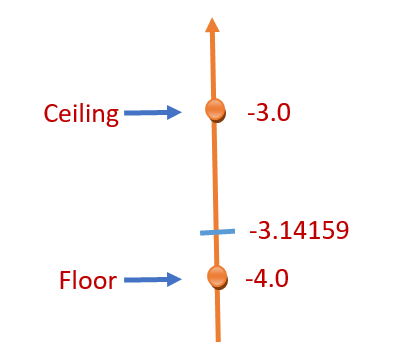
\includegraphics[width=0.35\linewidth]{img02/w02-floorCeilingFun} \end{center}

\begin{Shaded}
\begin{Highlighting}[]
\FunctionTok{ceiling}\NormalTok{(}\FloatTok{3.14159}\NormalTok{)}
\end{Highlighting}
\end{Shaded}

\begin{verbatim}
## [1] 4
\end{verbatim}

\begin{Shaded}
\begin{Highlighting}[]
\FunctionTok{ceiling}\NormalTok{(}\SpecialCharTok{{-}}\FloatTok{3.14159}\NormalTok{)}
\end{Highlighting}
\end{Shaded}

\begin{verbatim}
## [1] -3
\end{verbatim}

\hypertarget{trunc}{%
\subsection{\texorpdfstring{\texttt{trunc()}}{trunc()}}\label{trunc}}

\texttt{trunc()} is a rounding function with the format of \texttt{trunc(number)} that \textbf{drops all digits after the decimal point}.

\begin{Shaded}
\begin{Highlighting}[]
\FunctionTok{trunc}\NormalTok{(}\FloatTok{3.14159}\NormalTok{)}
\end{Highlighting}
\end{Shaded}

\begin{verbatim}
## [1] 3
\end{verbatim}

\begin{Shaded}
\begin{Highlighting}[]
\FunctionTok{trunc}\NormalTok{(}\SpecialCharTok{{-}}\FloatTok{3.14159}\NormalTok{)}
\end{Highlighting}
\end{Shaded}

\begin{verbatim}
## [1] -3
\end{verbatim}

\hypertarget{control-statements}{%
\section{Control Statements}\label{control-statements}}

Control statements are expressions used to control the execution and flow of the program based on the conditions provided in the statements. These structures are used to decide after assessing the variable.

There are 8 types of control statements in R:

\begin{itemize}
\tightlist
\item
  \texttt{if} condition
\item
  \texttt{if-else} condition
\item
  \texttt{for\ loop}
\item
  nested loops
\item
  \texttt{while\ loop}
\item
  \texttt{repeat} and \texttt{break} statements
\item
  \texttt{return} statement
\item
  \texttt{next} statement
\end{itemize}

We will introduce \texttt{if/if-else} statements and \texttt{for/while} loops in this note and use them to implement the algorithm with the given pseudo-code given in the lecture note.

\hfill\break

\hypertarget{conditional-statements}{%
\subsection{Conditional Statements}\label{conditional-statements}}

\hypertarget{if-statement}{%
\subsubsection{IF Statement}\label{if-statement}}

This control structure checks whether the expression provided in parenthesis is true or not. If true, the execution of the statements in braces \texttt{\{\}} continues. The syntax is given by

\textbf{Syntax}:

\begin{verbatim}
if(expression){
    statements
    ....
    ....
}
\end{verbatim}

\textbf{Example 1}:

\begin{Shaded}
\begin{Highlighting}[]
\NormalTok{x }\OtherTok{\textless{}{-}} \DecValTok{100}                              \CommentTok{\# numerical scalar}
\DocumentationTok{\#\#  }
\ControlFlowTok{if}\NormalTok{(x }\SpecialCharTok{\textgreater{}} \DecValTok{10}\NormalTok{)\{                           }\CommentTok{\# conditional statement}
\FunctionTok{print}\NormalTok{(}\FunctionTok{paste}\NormalTok{(x, }\StringTok{"is greater than 10"}\NormalTok{)) }\CommentTok{\# paste() is a string function. one }
                                      \CommentTok{\# can pass a numerical argument to}
                                      \CommentTok{\# this string function.}
\NormalTok{\}}
\end{Highlighting}
\end{Shaded}

\begin{verbatim}
## [1] "100 is greater than 10"
\end{verbatim}

\textbf{Example 2}:

\begin{Shaded}
\begin{Highlighting}[]
\NormalTok{x }\OtherTok{\textless{}{-}}\NormalTok{ pi                       }\CommentTok{\# numerical scalar}
\DocumentationTok{\#\#  }
\ControlFlowTok{if}\NormalTok{(x }\SpecialCharTok{==} \FloatTok{3.14159}\NormalTok{)\{             }\CommentTok{\# conditional statement}
\FunctionTok{print}\NormalTok{(}\FunctionTok{paste}\NormalTok{(x, }\StringTok{"is pi!"}\NormalTok{))  }
\NormalTok{\}}
\end{Highlighting}
\end{Shaded}

\hypertarget{if-else-statement}{%
\subsubsection{IF-ELSE Statement}\label{if-else-statement}}

If the \textbf{if condition} is determined as true, it will execute the statements written \emph{inside the if block}. Otherwise, if the \textbf{if condition} is not satisfied, it will return the statements written inside the \emph{else block}.

\textbf{Syntax}

\begin{verbatim}
if (condition) {# The statement will execute 
                # if the condition is satisfied.
     statement_1 
     ...........
   }
else { # The statement will execute if the condition 
       # turns out to be not satisfied. 
   statement_2 
   ...........
 }
\end{verbatim}

\textbf{Example 3}

\begin{Shaded}
\begin{Highlighting}[]
\NormalTok{x }\OtherTok{\textless{}{-}}\NormalTok{ pi                       }\CommentTok{\# numerical scalar}
\DocumentationTok{\#\#  }
\ControlFlowTok{if}\NormalTok{(x }\SpecialCharTok{==} \FloatTok{3.14159}\NormalTok{)\{             }\CommentTok{\# conditional statement}
   \FunctionTok{print}\NormalTok{(}\FunctionTok{paste}\NormalTok{(x, }\StringTok{"is pi!"}\NormalTok{))  }
\NormalTok{   \} }\ControlFlowTok{else}\NormalTok{ \{}
   \FunctionTok{print}\NormalTok{(}\FunctionTok{paste}\NormalTok{(x, }\StringTok{"is NOT pi!"}\NormalTok{))  }\CommentTok{\# Caution: x will be printed as a string!}
\NormalTok{  \}}
\end{Highlighting}
\end{Shaded}

\begin{verbatim}
## [1] "3.14159265358979 is NOT pi!"
\end{verbatim}

\hypertarget{else-if-statement}{%
\subsubsection{ELSE-IF Statement}\label{else-if-statement}}

It continuously checks certain conditions. If any of the if the condition is satisfied, it will return statements written inside the block. If none of the if the condition is true, it will execute the statements written inside the else block.

\textbf{Syntax}

\begin{verbatim}
if (condition){
     expression
  } else if (condition){
     expression
  } else if (condition){
     expression
  } else { # The statement will execute if none of the if 
           # conditions turn out to be true.
    statement 
}
\end{verbatim}

\textbf{Example 4}

\begin{Shaded}
\begin{Highlighting}[]
\NormalTok{y }\OtherTok{=} \DecValTok{10}

\ControlFlowTok{if}\NormalTok{ (x }\SpecialCharTok{\textgreater{}}\NormalTok{ y) \{                     }
    \FunctionTok{print}\NormalTok{(x)}
\NormalTok{\} }\ControlFlowTok{else} \ControlFlowTok{if}\NormalTok{ (y }\SpecialCharTok{==}\NormalTok{ x) \{}
    \FunctionTok{print}\NormalTok{(}\StringTok{"x and y are equal"}\NormalTok{)}
\NormalTok{\} }\ControlFlowTok{else}\NormalTok{ \{                         }
    \FunctionTok{print}\NormalTok{(y)}
\NormalTok{\}}
\end{Highlighting}
\end{Shaded}

\begin{verbatim}
## [1] 10
\end{verbatim}

\hfill\break

\hypertarget{loops-in-r}{%
\subsection{Loops in R}\label{loops-in-r}}

A loop is used to perform repetitive tasks. There are three types of loops in R: for-loop, while-loop, and repeat-while-loop. These loops are used with \texttt{if-else} like conditional statements to execute statements conditionally.

\hypertarget{for-loops}{%
\subsubsection{FOR Loops}\label{for-loops}}

A \textbf{for-loop} will run statements a pre-set number of times n.

\textbf{Syntax}

\begin{verbatim}
 for (i in 1:n){
  executable statements 
 }
\end{verbatim}

\textbf{Example 5}

Find 10 factorial (\(10!\)). Note that \(10! = 0\times 1\times 2\times \cdots \times 9 \times 10\). We only need 10 iterations of the cumulative product to find the value.

\begin{Shaded}
\begin{Highlighting}[]
\NormalTok{result }\OtherTok{=} \DecValTok{1}  \CommentTok{\# initial value to start the process of iteration}
\ControlFlowTok{for}\NormalTok{(i }\ControlFlowTok{in} \DecValTok{1}\SpecialCharTok{:}\DecValTok{10}\NormalTok{)\{}
\NormalTok{  result }\OtherTok{=}\NormalTok{ result }\SpecialCharTok{*}\NormalTok{ i}
\NormalTok{\}}
\FunctionTok{cat}\NormalTok{(}\StringTok{"}\SpecialCharTok{\textbackslash{}n}\StringTok{ 10! ="}\NormalTok{, result,}\StringTok{".}\SpecialCharTok{\textbackslash{}n}\StringTok{"}\NormalTok{)}
\end{Highlighting}
\end{Shaded}

\begin{verbatim}
## 
##  10! = 3628800 .
\end{verbatim}

\texttt{for-loop} is usually used jointly with other conditional statements defined by \texttt{if-else}, \texttt{break}, \texttt{next}, etc.

\textbf{Example 6}. Let X =c(10 18 42 46 11 29 15 22 20 8 49 47 1 16 23 13 32 27 19 37 31 43 39 24 44 12 3 2 9 7 50 4 30 6 45 38 17 14 26 36 21 41 40 5 33 34 25 28 35 48). We want to select 10 smallest odd numbers and store them in a vector.

\begin{Shaded}
\begin{Highlighting}[]
\CommentTok{\# define the vector}
\NormalTok{ X}\OtherTok{=}\FunctionTok{c}\NormalTok{(}\DecValTok{10}\NormalTok{, }\DecValTok{18}\NormalTok{, }\DecValTok{42}\NormalTok{, }\DecValTok{46}\NormalTok{, }\DecValTok{11}\NormalTok{, }\DecValTok{29}\NormalTok{, }\DecValTok{15}\NormalTok{, }\DecValTok{22}\NormalTok{, }\DecValTok{20}\NormalTok{, }\DecValTok{8}\NormalTok{, }\DecValTok{49}\NormalTok{, }\DecValTok{47}\NormalTok{, }\DecValTok{1}\NormalTok{, }\DecValTok{16}\NormalTok{, }\DecValTok{23}\NormalTok{, }\DecValTok{13}\NormalTok{, }\DecValTok{32}\NormalTok{, }\DecValTok{27}\NormalTok{,}
     \DecValTok{19}\NormalTok{, }\DecValTok{37}\NormalTok{, }\DecValTok{31}\NormalTok{, }\DecValTok{43}\NormalTok{, }\DecValTok{39}\NormalTok{, }\DecValTok{24}\NormalTok{, }\DecValTok{44}\NormalTok{, }\DecValTok{12}\NormalTok{, }\DecValTok{3}\NormalTok{, }\DecValTok{2}\NormalTok{, }\DecValTok{9}\NormalTok{, }\DecValTok{7}\NormalTok{, }\DecValTok{50}\NormalTok{, }\DecValTok{4}\NormalTok{, }\DecValTok{30}\NormalTok{, }\DecValTok{6}\NormalTok{, }\DecValTok{45}\NormalTok{, }\DecValTok{38}\NormalTok{, }\DecValTok{17}\NormalTok{,}
     \DecValTok{14}\NormalTok{, }\DecValTok{26}\NormalTok{, }\DecValTok{36}\NormalTok{, }\DecValTok{21}\NormalTok{, }\DecValTok{41}\NormalTok{, }\DecValTok{40}\NormalTok{, }\DecValTok{5}\NormalTok{, }\DecValTok{33}\NormalTok{, }\DecValTok{34}\NormalTok{, }\DecValTok{25}\NormalTok{, }\DecValTok{28}\NormalTok{, }\DecValTok{35}\NormalTok{, }\DecValTok{48}\NormalTok{)}
\CommentTok{\# Note that the largest of the first 10 smallest odd number is 19.}
\NormalTok{oddVec }\OtherTok{=} \ConstantTok{NULL}     \CommentTok{\# store the first 10 smallest odd numbers}
\NormalTok{k }\OtherTok{=} \DecValTok{1}             \CommentTok{\# initial index of oddVec}
\ControlFlowTok{for}\NormalTok{ (i }\ControlFlowTok{in} \DecValTok{1}\SpecialCharTok{:}\DecValTok{100}\NormalTok{)\{}
\NormalTok{     xi }\OtherTok{=}\NormalTok{ X[i]}
\NormalTok{     I }\OtherTok{=}\NormalTok{ X[i]}\SpecialCharTok{\%\%}\DecValTok{2}         \CommentTok{\# \%\% gives the remainder of the division }
     \ControlFlowTok{if}\NormalTok{(I }\SpecialCharTok{==} \DecValTok{0}\NormalTok{)\{}
         \ControlFlowTok{next}            \CommentTok{\# skip the current iteration and jump to the next}
\NormalTok{     \} }\ControlFlowTok{else}\NormalTok{\{}
        \ControlFlowTok{if}\NormalTok{(xi }\SpecialCharTok{\textgreater{}} \DecValTok{19}\NormalTok{) \{}
           \ControlFlowTok{next}          \CommentTok{\# skip the current iteration and jump to the next}
\NormalTok{       \} }\ControlFlowTok{else}\NormalTok{\{}
\NormalTok{           oddVec[k] }\OtherTok{=}\NormalTok{ xi}
           \ControlFlowTok{if}\NormalTok{ (k }\SpecialCharTok{==} \DecValTok{10}\NormalTok{) }\ControlFlowTok{break}    \CommentTok{\# beak the iteration once all }
                                 \CommentTok{\# desired odd numbers are selected!}
\NormalTok{           k }\OtherTok{=}\NormalTok{ k }\SpecialCharTok{+} \DecValTok{1}             \CommentTok{\# update the index for the next valid odd number}
\NormalTok{       \}}
\NormalTok{     \}}
\NormalTok{  \}}
\NormalTok{oddVec}
\end{Highlighting}
\end{Shaded}

\begin{verbatim}
##  [1] 11 15  1 13 19  3  9  7 17  5
\end{verbatim}

\hypertarget{while-loops}{%
\subsubsection{WHILE Loops}\label{while-loops}}

The while loop repeats statements as long as a certain condition is true. Stated another way, the while loop will stop when the condition is false (for example, the user types 0 to exit). Each time the loop starts running, it checks the condition.

See the example in the next section.

\hypertarget{repeat-if-while-loops}{%
\subsubsection{REPEAT-IF-WHILE Loops}\label{repeat-if-while-loops}}

This loop is equivalent to the \textbf{DO-WHILE} loop in other languages such as SAS and
C++.

The \texttt{repeat\ loop} does not have any condition to \textbf{terminate} the loop. We need to put an \textbf{exit condition} implicitly with a \textbf{break statement} inside the loop.

\hfill\break

\textbf{Syntax}:

\begin{verbatim}
repeat{
  statements...
  if(condition){
    break
  }
}
\end{verbatim}

\textbf{Example 6}

\begin{Shaded}
\begin{Highlighting}[]
\NormalTok{i }\OtherTok{=} \DecValTok{1}
\ControlFlowTok{repeat}\NormalTok{ \{}
  \FunctionTok{print}\NormalTok{(i)}
\NormalTok{  i }\OtherTok{=}\NormalTok{ i }\SpecialCharTok{+} \DecValTok{1}
  \ControlFlowTok{if}\NormalTok{(i }\SpecialCharTok{\textgreater{}=} \DecValTok{5}\NormalTok{ )}
    \ControlFlowTok{break}
\NormalTok{\}}
\end{Highlighting}
\end{Shaded}

\begin{verbatim}
## [1] 1
## [1] 2
## [1] 3
## [1] 4
\end{verbatim}

\hfill\break

\hypertarget{numerical-example}{%
\section{Numerical Example}\label{numerical-example}}

\textbf{Example 4 (Numerical Implementation)}: The nth Taylor polynomial for \(f (x) = e^x\) expanded about \(x_0 = 0\) is
\[
P_n(x) =\sum_{i=0}^n \frac{x^i}{i!}
\]
and the value of \(e\) to six decimal places is 2.718282. \textbf{Construct an algorithm} to determine the \textbf{minimal value of \(n\)} required for
\[
|e - P_n(1)| < 10^{-5},
\]
without using the Taylor polynomial remainder term.

\textbf{Solution}: The objective is to determine the degrees of the Taylor polynomial evaluated at \(x = 1\) to approximate \(e\). The input values are (1) tolerance TOL and the initial degree of the Taylor polynomial. The output is the smallest degree of the Taylor polynomial that meets \(|e - P_n(1)| < TOL\).

\textbf{Caution}: In general, one should consider including two stopping rules: error tolerance and maximum iterations. In this particular example, the maximum number of iterations is simply the solution to the problem. Therefore, there is one stopping rule: TOL

\hfill\break

\hypertarget{version-1}{%
\subsection{VERSION 1}\label{version-1}}

This is modified from the pseudo-code from the example in the lecture note.

\begin{verbatim}
INPUT  initial degree: n, 
            tolerance: TOL, 
            
OUTPUT the desired degree N of the polynomial

Step 1. SET   n = 0;
             Pn = 1; 
            ERR = exp(1) - 1;
Step 2. WHILE ERR >= TOL DO:
        1.   n = n + 1
            Pn = Pn + 1/n!         # n! = n factorial
           ERR = exp(1) - Pn       # exp(1) = 2.718282
        2. IF |ERR| < TOL DO:
               OUTPUT (N)
               WRITE (tolerance achieved!)
               STOP
           ELSE DO:               # optional: print out something
                                  # to monitor the iterative process
               WRITE(iteration number)
          ENDIF
        ENDWHILE
\end{verbatim}

\hfill\break

The following is the R code for implementing the above pseudo-code.

\begin{Shaded}
\begin{Highlighting}[]
\NormalTok{ n }\OtherTok{=} \DecValTok{0}
\NormalTok{ TOL }\OtherTok{=} \DecValTok{10}\SpecialCharTok{\^{}}\NormalTok{(}\SpecialCharTok{{-}}\DecValTok{5}\NormalTok{)}
\NormalTok{ Pn }\OtherTok{=} \DecValTok{1}
\NormalTok{ ERR }\OtherTok{=} \FunctionTok{exp}\NormalTok{(}\DecValTok{1}\NormalTok{) }\SpecialCharTok{{-}}\NormalTok{ Pn}
\CommentTok{\# Loop Starts}
\ControlFlowTok{while}\NormalTok{(ERR }\SpecialCharTok{\textgreater{}=}\NormalTok{ TOL)\{}
\NormalTok{  n }\OtherTok{=}\NormalTok{ n }\SpecialCharTok{+} \DecValTok{1}
\NormalTok{  Pn }\OtherTok{=}\NormalTok{ Pn }\SpecialCharTok{+} \DecValTok{1}\SpecialCharTok{/}\FunctionTok{factorial}\NormalTok{(n)}
\NormalTok{  ERR }\OtherTok{=} \FunctionTok{exp}\NormalTok{(}\DecValTok{1}\NormalTok{) }\SpecialCharTok{{-}}\NormalTok{ Pn}
  \ControlFlowTok{if}\NormalTok{(ERR }\SpecialCharTok{\textless{}}\NormalTok{ TOL)\{}
  \FunctionTok{cat}\NormalTok{(}\StringTok{"}\SpecialCharTok{\textbackslash{}n\textbackslash{}n}\StringTok{ The desired degrees of the Taylor polynomial is "}\NormalTok{, n}\SpecialCharTok{+}\DecValTok{1}\NormalTok{,}\StringTok{". }\SpecialCharTok{\textbackslash{}n}\StringTok{"}\NormalTok{)  }
  \FunctionTok{cat}\NormalTok{(}\StringTok{"Tolerance achieved!}\SpecialCharTok{\textbackslash{}n\textbackslash{}n\textbackslash{}n}\StringTok{"}\NormalTok{)  }
\NormalTok{  \} }\ControlFlowTok{else}\NormalTok{\{}
  \FunctionTok{cat}\NormalTok{(}\StringTok{"}\SpecialCharTok{\textbackslash{}n}\StringTok{ Iteration number: "}\NormalTok{, n, }\StringTok{". "}\NormalTok{) }
\NormalTok{  \}}
\NormalTok{ \}}
\end{Highlighting}
\end{Shaded}

\begin{verbatim}
## 
##  Iteration number:  1 . 
##  Iteration number:  2 . 
##  Iteration number:  3 . 
##  Iteration number:  4 . 
##  Iteration number:  5 . 
##  Iteration number:  6 . 
##  Iteration number:  7 . 
## 
##  The desired degrees of the Taylor polynomial is  9 . 
## Tolerance achieved!
\end{verbatim}

\hypertarget{version-2}{%
\subsection{Version 2}\label{version-2}}

Change the order for updating the degrees of the polynomial and add additional outputs

\begin{verbatim}
INPUT  initial degree: n, 
            tolerance: TOL, 
            
OUTPUT the desired degree N of the polynomial

Step 1. SET   n = 0;
             Pn = 0; 
            ERR = exp(1);
Step 2. WHILE ERR >= TOL DO:
        1.  Pn = Pn + 1/n!         # n! = n factorial
           ERR = exp(1) - Pn       # exp(1) = 2.718282
        2. IF |ERR| < TOL DO:
               OUTPUT (N, Pn, absolute error)
               WRITE (tolerance achieved!)
               STOP
           ELSE DO:               # optional: print out something
                                  # to monitor the iterative process
               WRITE (iteration number, absolute error)
               n = n + 1
          ENDIF
        ENDWHILE
\end{verbatim}

\hfill\break

The following is the R code for implementing the above pseudo-code.

\begin{Shaded}
\begin{Highlighting}[]
\NormalTok{ n }\OtherTok{=} \DecValTok{0}
\NormalTok{ TOL }\OtherTok{=} \DecValTok{10}\SpecialCharTok{\^{}}\NormalTok{(}\SpecialCharTok{{-}}\DecValTok{5}\NormalTok{)}
\NormalTok{ Pn }\OtherTok{=} \DecValTok{0}
\NormalTok{ ERR }\OtherTok{=} \FunctionTok{exp}\NormalTok{(}\DecValTok{1}\NormalTok{) }
\CommentTok{\# Loop Starts}
\ControlFlowTok{while}\NormalTok{(ERR }\SpecialCharTok{\textgreater{}=}\NormalTok{ TOL)\{}
\NormalTok{  Pn }\OtherTok{=}\NormalTok{ Pn }\SpecialCharTok{+} \DecValTok{1}\SpecialCharTok{/}\FunctionTok{factorial}\NormalTok{(n)}
\NormalTok{  ERR }\OtherTok{=} \FunctionTok{exp}\NormalTok{(}\DecValTok{1}\NormalTok{) }\SpecialCharTok{{-}}\NormalTok{ Pn}
  \ControlFlowTok{if}\NormalTok{(ERR }\SpecialCharTok{\textless{}}\NormalTok{ TOL)\{}
     \FunctionTok{cat}\NormalTok{(}\StringTok{"}\SpecialCharTok{\textbackslash{}n\textbackslash{}n}\StringTok{Tolerance achieved!}\SpecialCharTok{\textbackslash{}n\textbackslash{}n}\StringTok{"}\NormalTok{)  }
     \FunctionTok{cat}\NormalTok{(}\StringTok{"}\SpecialCharTok{\textbackslash{}n}\StringTok{ degree N = "}\NormalTok{, n}\SpecialCharTok{+}\DecValTok{1}\NormalTok{, }\StringTok{"."}\NormalTok{)}
     \FunctionTok{cat}\NormalTok{(}\StringTok{"}\SpecialCharTok{\textbackslash{}n}\StringTok{ e = "}\NormalTok{, }\FunctionTok{exp}\NormalTok{(}\DecValTok{1}\NormalTok{), }\StringTok{"."}\NormalTok{)}
     \FunctionTok{cat}\NormalTok{(}\StringTok{"}\SpecialCharTok{\textbackslash{}n}\StringTok{ Pn ="}\NormalTok{, Pn, }\StringTok{"."}\NormalTok{)}
     \FunctionTok{cat}\NormalTok{(}\StringTok{"}\SpecialCharTok{\textbackslash{}n}\StringTok{ Absolute Error ="}\NormalTok{, ERR, }\StringTok{"."}\NormalTok{)     }
\NormalTok{  \} }\ControlFlowTok{else}\NormalTok{\{}
\NormalTok{          n }\OtherTok{=}\NormalTok{ n }\SpecialCharTok{+} \DecValTok{1}
     \FunctionTok{cat}\NormalTok{(}\StringTok{"}\SpecialCharTok{\textbackslash{}n}\StringTok{ Iteration numer: "}\NormalTok{, n, }\StringTok{". Absolute Error = "}\NormalTok{, ERR, }\StringTok{"."}\NormalTok{) }
\NormalTok{  \}}
\NormalTok{ \}}
\end{Highlighting}
\end{Shaded}

\begin{verbatim}
## 
##  Iteration numer:  1 . Absolute Error =  1.718282 .
##  Iteration numer:  2 . Absolute Error =  0.7182818 .
##  Iteration numer:  3 . Absolute Error =  0.2182818 .
##  Iteration numer:  4 . Absolute Error =  0.05161516 .
##  Iteration numer:  5 . Absolute Error =  0.009948495 .
##  Iteration numer:  6 . Absolute Error =  0.001615162 .
##  Iteration numer:  7 . Absolute Error =  0.0002262729 .
##  Iteration numer:  8 . Absolute Error =  2.786021e-05 .
## 
## Tolerance achieved!
## 
## 
##  degree N =  9 .
##  e =  2.718282 .
##  Pn = 2.718279 .
##  Absolute Error = 3.058618e-06 .
\end{verbatim}

\hypertarget{user-defined-functions}{%
\section{User Defined Functions}\label{user-defined-functions}}

One of the great strengths of R is that it allows users to extend the capacity of R through user-defined functions. Functions are often used to encapsulate a sequence of expressions that need to be executed repetitively. We have made code to implement bisection and fixed-point methods by specific examples. We may want to write the R function of these implementations so we can use them for other root-finding problems with the appropriate input information.

The syntax of the general user-defined R function has the following form

\begin{verbatim}
myfunction <- function(arg1, arg2, ... ){
   statements
   return(object)
}
\end{verbatim}

\texttt{arg1,\ arg2,\ ...} are arguments that are passed into the function. The arguments could be any objects such as vectors and other user-defined R functions.

\textbf{Example 1} Finding the standard deviation of an input vector.

\begin{Shaded}
\begin{Highlighting}[]
\NormalTok{sdfun }\OtherTok{\textless{}{-}} \ControlFlowTok{function}\NormalTok{(x) \{}
\NormalTok{  res }\OtherTok{\textless{}{-}} \FunctionTok{sqrt}\NormalTok{(}\FunctionTok{sum}\NormalTok{((x }\SpecialCharTok{{-}} \FunctionTok{mean}\NormalTok{(x))}\SpecialCharTok{\^{}}\DecValTok{2}\NormalTok{) }\SpecialCharTok{/}\NormalTok{ (}\FunctionTok{length}\NormalTok{(x) }\SpecialCharTok{{-}} \DecValTok{1}\NormalTok{))}
  \FunctionTok{return}\NormalTok{(res)}
\NormalTok{\}}
\DocumentationTok{\#\#}
\NormalTok{vec }\OtherTok{=} \FunctionTok{c}\NormalTok{(}\DecValTok{1}\NormalTok{,}\DecValTok{4}\NormalTok{,}\DecValTok{2}\NormalTok{,}\DecValTok{6}\NormalTok{,}\SpecialCharTok{{-}}\DecValTok{3}\NormalTok{, }\SpecialCharTok{{-}}\DecValTok{5}\NormalTok{)}
\FunctionTok{sdfun}\NormalTok{(}\AttributeTok{x =}\NormalTok{ vec)   }\CommentTok{\# or simply sdfun(vec)}
\end{Highlighting}
\end{Shaded}

\begin{verbatim}
## [1] 4.167333
\end{verbatim}

We have defined functions in implementing root-finding methods.

\hfill\break

\hypertarget{writing-r-functions-for-root-finding-methods}{%
\subsection{Writing R Functions for Root-finding Methods}\label{writing-r-functions-for-root-finding-methods}}

As an example, we will write an R function to implement the bisection method for finding the root for any given equation on ver an interval (if it exists). Two versions of R functions will be presented in the following.

\hypertarget{function-with-numerical-outputs}{%
\subsubsection{Function with Numerical Outputs}\label{function-with-numerical-outputs}}

We simply wrap up the example code in the lecture note to make the following function.

\begin{Shaded}
\begin{Highlighting}[]
\NormalTok{num.FixedPoint }\OtherTok{=} \ControlFlowTok{function}\NormalTok{(fn,       }\CommentTok{\# function that satisfies f(x) = x}
\NormalTok{                          a,        }\CommentTok{\# lower limit of the interval [a, b]}
\NormalTok{                          b,        }\CommentTok{\# upper limit of the interval [a, b]}
\NormalTok{                          TOL,      }\CommentTok{\# error tolerance}
\NormalTok{                          N,        }\CommentTok{\# maximum number of iterations}
\NormalTok{                          x0,       }\CommentTok{\# initial value of x}
\NormalTok{                          detail,    }\CommentTok{\# intermediate output}
\NormalTok{                          ...)\{}
\NormalTok{ gfun }\OtherTok{=}\NormalTok{ fn}
\NormalTok{ x }\OtherTok{=}\NormalTok{ x0}
\NormalTok{ ERR }\OtherTok{=} \ConstantTok{Inf}
\NormalTok{ n }\OtherTok{=} \DecValTok{0}
\DocumentationTok{\#\# }
 \ControlFlowTok{while}\NormalTok{ (ERR }\SpecialCharTok{\textgreater{}}\NormalTok{ TOL)\{}
\NormalTok{  n }\OtherTok{=}\NormalTok{ n }\SpecialCharTok{+} \DecValTok{1}
\NormalTok{  new.x }\OtherTok{=} \FunctionTok{gfun}\NormalTok{(x)}
\NormalTok{  ERR }\OtherTok{=} \FunctionTok{abs}\NormalTok{(new.x }\SpecialCharTok{{-}}\NormalTok{ x)}
  \ControlFlowTok{if}\NormalTok{(ERR }\SpecialCharTok{\textless{}}\NormalTok{ TOL)\{}
    \FunctionTok{cat}\NormalTok{(}\StringTok{"}\SpecialCharTok{\textbackslash{}n\textbackslash{}n}\StringTok{The algorithm converges!"}\NormalTok{)}
    \FunctionTok{cat}\NormalTok{(}\StringTok{"}\SpecialCharTok{\textbackslash{}n}\StringTok{The approximate root is:"}\NormalTok{, new.x,}\StringTok{"."}\NormalTok{)}
    \FunctionTok{cat}\NormalTok{(}\StringTok{"}\SpecialCharTok{\textbackslash{}n}\StringTok{The absolute error is:"}\NormalTok{, ERR, }\StringTok{"."}\NormalTok{)}
    \FunctionTok{cat}\NormalTok{(}\StringTok{"}\SpecialCharTok{\textbackslash{}n}\StringTok{The number of iterations is:"}\NormalTok{, n, }\StringTok{"."}\NormalTok{)}
    \ControlFlowTok{break}
\NormalTok{  \} }\ControlFlowTok{else}\NormalTok{\{}
    \ControlFlowTok{if}\NormalTok{(ERR }\SpecialCharTok{\textgreater{}} \DecValTok{10}\SpecialCharTok{\^{}}\DecValTok{7}\NormalTok{)\{}
        \FunctionTok{cat}\NormalTok{(}\StringTok{"}\SpecialCharTok{\textbackslash{}n\textbackslash{}n}\StringTok{The algorithm diverges!"}\NormalTok{)}
        \ControlFlowTok{break}
\NormalTok{    \} }\ControlFlowTok{else}\NormalTok{\{}
         \ControlFlowTok{if}\NormalTok{(detail }\SpecialCharTok{==} \ConstantTok{TRUE}\NormalTok{)\{}
            \FunctionTok{cat}\NormalTok{(}\StringTok{"}\SpecialCharTok{\textbackslash{}n}\StringTok{Iteration:"}\NormalTok{,n,}\StringTok{". Estimated root:"}\NormalTok{, new.x, }\StringTok{". Absolute error:"}\NormalTok{, ERR,}\StringTok{"."}\NormalTok{)}
\NormalTok{          \}}
\NormalTok{         x }\OtherTok{=}\NormalTok{ new.x         }\CommentTok{\# update x value!!!}
\NormalTok{    \}}
\NormalTok{  \}}
  \ControlFlowTok{if}\NormalTok{(n }\SpecialCharTok{==}\NormalTok{ N)\{}
    \FunctionTok{cat}\NormalTok{(}\StringTok{"}\SpecialCharTok{\textbackslash{}n\textbackslash{}n}\StringTok{The maximum number of iterations is achieved!"}\NormalTok{)}
    \ControlFlowTok{break}
\NormalTok{  \} }
\NormalTok{ \}}
\NormalTok{\}}
\end{Highlighting}
\end{Shaded}

Next, we use several examples.

\textbf{Example 1} Using the fixed-point method to find the approximate root of \(x^3 - 7x +2 = 0\). To use the fixed-point method, we rewrite the equation into the form \((x^3 + 2)/7 = x\). Then \(g(x) = (x^3 + 2)/7\) will be the function to be passed into the function.

\begin{Shaded}
\begin{Highlighting}[]
\DocumentationTok{\#\#\#}
\NormalTok{fun0 }\OtherTok{=} \ControlFlowTok{function}\NormalTok{(x) (x}\SpecialCharTok{\^{}}\DecValTok{3} \SpecialCharTok{+} \DecValTok{2}\NormalTok{)}\SpecialCharTok{/}\DecValTok{7}
\FunctionTok{num.FixedPoint}\NormalTok{(}\AttributeTok{fn =}\NormalTok{ fun0, }\AttributeTok{a =} \DecValTok{0}\NormalTok{, }\AttributeTok{b =} \DecValTok{2}\NormalTok{, }\AttributeTok{TOL =} \DecValTok{10}\SpecialCharTok{\^{}}\NormalTok{(}\SpecialCharTok{{-}}\DecValTok{6}\NormalTok{), }\AttributeTok{N =} \DecValTok{200}\NormalTok{, }\AttributeTok{x0 =}\FloatTok{1.5}\NormalTok{, }\AttributeTok{detail =} \ConstantTok{TRUE}\NormalTok{)}
\end{Highlighting}
\end{Shaded}

\begin{verbatim}
## 
## Iteration: 1 . Estimated root: 0.7678571 . Absolute error: 0.7321429 .
## Iteration: 2 . Estimated root: 0.3503903 . Absolute error: 0.4174668 .
## Iteration: 3 . Estimated root: 0.2918598 . Absolute error: 0.0585305 .
## Iteration: 4 . Estimated root: 0.2892659 . Absolute error: 0.002593907 .
## Iteration: 5 . Estimated root: 0.289172 . Absolute error: 9.385572e-05 .
## Iteration: 6 . Estimated root: 0.2891687 . Absolute error: 3.364631e-06 .
## 
## The algorithm converges!
## The approximate root is: 0.2891686 .
## The absolute error is: 1.20578e-07 .
## The number of iterations is: 7 .
\end{verbatim}

\textbf{Example 2}: Calculate \(1/\sqrt{2}\) by using the fixed-point method. Note that \(f(x) = x^2 - 1/2\). To use the fixed point method, we need \(g(x) = x -x^2 +1/2\) as the input function.

\begin{Shaded}
\begin{Highlighting}[]
\DocumentationTok{\#\#\#}
\NormalTok{fun0 }\OtherTok{=} \ControlFlowTok{function}\NormalTok{(x) x }\SpecialCharTok{{-}}\NormalTok{ x}\SpecialCharTok{\^{}}\DecValTok{3} \SpecialCharTok{+} \DecValTok{1}\SpecialCharTok{/}\DecValTok{2}
\FunctionTok{num.FixedPoint}\NormalTok{(}\AttributeTok{fn =}\NormalTok{ fun0, }\AttributeTok{a =} \SpecialCharTok{{-}}\DecValTok{1}\NormalTok{, }\AttributeTok{b =} \DecValTok{2}\NormalTok{, }\AttributeTok{TOL =} \DecValTok{10}\SpecialCharTok{\^{}}\NormalTok{(}\SpecialCharTok{{-}}\DecValTok{5}\NormalTok{), }\AttributeTok{N =} \DecValTok{200}\NormalTok{, }\AttributeTok{x0 =}\FloatTok{0.7}\NormalTok{, }\AttributeTok{detail =}\ConstantTok{FALSE}\NormalTok{)}
\end{Highlighting}
\end{Shaded}

\begin{verbatim}
## 
## 
## The algorithm converges!
## The approximate root is: 0.7937048 .
## The absolute error is: 9.128962e-06 .
## The number of iterations is: 83 .
\end{verbatim}

\hypertarget{function-with-more-optional-outputs}{%
\subsubsection{Function with More Optional Outputs}\label{function-with-more-optional-outputs}}

We include graphics the function created previously.

\begin{Shaded}
\begin{Highlighting}[]
\NormalTok{FixedPointAlgR }\OtherTok{=} \ControlFlowTok{function}\NormalTok{(fn,       }\CommentTok{\# function that satisfies f(x) = x}
\NormalTok{                          a,        }\CommentTok{\# lower limit of the interval [a, b]}
\NormalTok{                          b,        }\CommentTok{\# upper limit of the interval [a, b]}
\NormalTok{                          TOL,      }\CommentTok{\# error tolerance}
\NormalTok{                          N,        }\CommentTok{\# maximum number of iterations}
\NormalTok{                          x0,       }\CommentTok{\# initial value of x}
                          \AttributeTok{detail=}\ConstantTok{TRUE}\NormalTok{,   }\CommentTok{\# intermediate numerical outputs}
                          \AttributeTok{graphic=}\ConstantTok{TRUE}\NormalTok{,  }\CommentTok{\# intermediate graphic outputs}
\NormalTok{                          x.lim,    }\CommentTok{\# x{-}axis of graphic window}
\NormalTok{                          y.lim,    }\CommentTok{\# y{-}axis of graphic window}
\NormalTok{                          sleep,    }\CommentTok{\# sleep time between iterations}
\NormalTok{                          ...)\{}
\NormalTok{ gfun }\OtherTok{=}\NormalTok{ fn      }\CommentTok{\# rename the input function used in the function}
\NormalTok{ x }\OtherTok{=}\NormalTok{ x0         }\CommentTok{\# rename the initial value used in the function}
\NormalTok{ ERR }\OtherTok{=} \ConstantTok{Inf}      \CommentTok{\# initial error (a big  number to start the iteration)}
\NormalTok{ n }\OtherTok{=} \DecValTok{0}          \CommentTok{\# initial iteration counter {-} iterator or index}
\DocumentationTok{\#\#}
 \ControlFlowTok{if}\NormalTok{(graphic}\SpecialCharTok{==}\ConstantTok{TRUE}\NormalTok{)\{}
\NormalTok{ xlimit}\OtherTok{=}\FunctionTok{c}\NormalTok{(a}\FloatTok{{-}0.1}\SpecialCharTok{*}\FunctionTok{abs}\NormalTok{(b}\SpecialCharTok{{-}}\NormalTok{a), b}\FloatTok{+0.1}\SpecialCharTok{*}\FunctionTok{abs}\NormalTok{(b}\SpecialCharTok{{-}}\NormalTok{a))               }\CommentTok{\# x{-}limit in the graphic window}
\NormalTok{ xx}\OtherTok{=}\FunctionTok{seq}\NormalTok{(a}\FloatTok{{-}0.1}\SpecialCharTok{*}\FunctionTok{abs}\NormalTok{(b}\SpecialCharTok{{-}}\NormalTok{a), b}\FloatTok{+0.1}\SpecialCharTok{*}\FunctionTok{abs}\NormalTok{(b}\SpecialCharTok{{-}}\NormalTok{a), }\AttributeTok{length =} \DecValTok{2000}\NormalTok{)  }\CommentTok{\# sequence of x values}
\NormalTok{ yy1 }\OtherTok{=} \FunctionTok{gfun}\NormalTok{(xx)                                         }\CommentTok{\# evaluate g(x)}
\NormalTok{ yy2 }\OtherTok{=}\NormalTok{ xx                                               }\CommentTok{\# evaluate diagonal}
 \FunctionTok{plot}\NormalTok{(xx, yy1, }\AttributeTok{ylim =}\NormalTok{ y.lim, }\AttributeTok{xlim =}\NormalTok{ x.lim, }\AttributeTok{type =} \StringTok{"l"}\NormalTok{, }\AttributeTok{lwd =} \DecValTok{2}\NormalTok{, }\AttributeTok{lty =} \DecValTok{1}\NormalTok{, }\AttributeTok{col =} \StringTok{"blue"}\NormalTok{)}
 \FunctionTok{lines}\NormalTok{(xx,yy2, }\AttributeTok{lwd =} \DecValTok{2}\NormalTok{, }\AttributeTok{lty =} \DecValTok{1}\NormalTok{, }\AttributeTok{col =}\StringTok{"darkred"}\NormalTok{)        }\CommentTok{\# add line y = x}
 \FunctionTok{title}\NormalTok{(}\StringTok{"Fixed Point Algorithm Approximation"}\NormalTok{)           }\CommentTok{\# add title to the graphic}
\NormalTok{ \}}
\DocumentationTok{\#\# }
 \ControlFlowTok{while}\NormalTok{ (ERR }\SpecialCharTok{\textgreater{}}\NormalTok{ TOL)\{}
  \FunctionTok{Sys.sleep}\NormalTok{(sleep)                                      }\CommentTok{\# put the system to sleep}
\NormalTok{  n }\OtherTok{=}\NormalTok{ n }\SpecialCharTok{+} \DecValTok{1}
\NormalTok{  new.x }\OtherTok{=} \FunctionTok{gfun}\NormalTok{(x)}
\NormalTok{  ERR }\OtherTok{=} \FunctionTok{abs}\NormalTok{(new.x }\SpecialCharTok{{-}}\NormalTok{ x)}
  \ControlFlowTok{if}\NormalTok{(ERR }\SpecialCharTok{\textless{}}\NormalTok{ TOL)\{}
    \FunctionTok{cat}\NormalTok{(}\StringTok{"}\SpecialCharTok{\textbackslash{}n\textbackslash{}n}\StringTok{The algorithm converges!"}\NormalTok{)}
    \FunctionTok{cat}\NormalTok{(}\StringTok{"}\SpecialCharTok{\textbackslash{}n}\StringTok{The approximate root is:"}\NormalTok{, new.x,}\StringTok{"."}\NormalTok{)}
    \FunctionTok{cat}\NormalTok{(}\StringTok{"}\SpecialCharTok{\textbackslash{}n}\StringTok{The absolute error is:"}\NormalTok{, ERR, }\StringTok{"."}\NormalTok{)}
    \FunctionTok{cat}\NormalTok{(}\StringTok{"}\SpecialCharTok{\textbackslash{}n}\StringTok{The number of iterations is:"}\NormalTok{, n, }\StringTok{"."}\NormalTok{)}
    \ControlFlowTok{break}
\NormalTok{  \} }\ControlFlowTok{else}\NormalTok{\{}
    \ControlFlowTok{if}\NormalTok{(ERR }\SpecialCharTok{\textgreater{}} \DecValTok{10}\SpecialCharTok{\^{}}\DecValTok{7}\NormalTok{)\{}
        \FunctionTok{cat}\NormalTok{(}\StringTok{"}\SpecialCharTok{\textbackslash{}n\textbackslash{}n}\StringTok{The algorithm diverges!"}\NormalTok{)}
        \ControlFlowTok{break}
\NormalTok{    \} }\ControlFlowTok{else}\NormalTok{\{}
         \ControlFlowTok{if}\NormalTok{(detail }\SpecialCharTok{==} \ConstantTok{TRUE}\NormalTok{)\{}
            \FunctionTok{cat}\NormalTok{(}\StringTok{"}\SpecialCharTok{\textbackslash{}n}\StringTok{Iteration:"}\NormalTok{,n,}\StringTok{". Estimated root:"}\NormalTok{, new.x, }\StringTok{". Absolute error:"}\NormalTok{, ERR,}\StringTok{"."}\NormalTok{)}
\NormalTok{         \}}
        \ControlFlowTok{if}\NormalTok{(graphic}\SpecialCharTok{==}\ConstantTok{TRUE}\NormalTok{)\{}
            \FunctionTok{segments}\NormalTok{(new.x, new.x,       new.x,       }\FunctionTok{gfun}\NormalTok{(new.x), }\AttributeTok{col=}\StringTok{"purple"}\NormalTok{)}
            \FunctionTok{segments}\NormalTok{(new.x, }\FunctionTok{gfun}\NormalTok{(new.x), }\FunctionTok{gfun}\NormalTok{(new.x), }\FunctionTok{gfun}\NormalTok{(new.x), }\AttributeTok{col=}\StringTok{"purple"}\NormalTok{)}
\NormalTok{           \}}

\NormalTok{         x }\OtherTok{=}\NormalTok{ new.x         }\CommentTok{\# update x value!!!}
\NormalTok{    \}}
\NormalTok{  \}}
  \ControlFlowTok{if}\NormalTok{(n }\SpecialCharTok{==}\NormalTok{ N)\{              }\CommentTok{\# checking iteration limit}
    \FunctionTok{cat}\NormalTok{(}\StringTok{"}\SpecialCharTok{\textbackslash{}n\textbackslash{}n}\StringTok{The maximum number of iterations is achieved!"}\NormalTok{)   }
    \ControlFlowTok{break}
\NormalTok{  \} }
\NormalTok{ \}}
\NormalTok{\}}
\end{Highlighting}
\end{Shaded}

\hfill\break

\textbf{Example 1} (Revisited)

\begin{Shaded}
\begin{Highlighting}[]
\DocumentationTok{\#\#\#}
\NormalTok{fun0 }\OtherTok{=} \ControlFlowTok{function}\NormalTok{(x) (x}\SpecialCharTok{\^{}}\DecValTok{3} \SpecialCharTok{+} \DecValTok{2}\NormalTok{)}\SpecialCharTok{/}\DecValTok{7}
\FunctionTok{FixedPointAlgR}\NormalTok{(}\AttributeTok{fn =}\NormalTok{ fun0, }\AttributeTok{a =} \DecValTok{0}\NormalTok{, }\AttributeTok{b =} \DecValTok{1}\NormalTok{, }\AttributeTok{TOL =} \DecValTok{10}\SpecialCharTok{\^{}}\NormalTok{(}\SpecialCharTok{{-}}\DecValTok{6}\NormalTok{), }\AttributeTok{N =} \DecValTok{200}\NormalTok{, }
               \AttributeTok{x0 =}\FloatTok{0.35}\NormalTok{, }\AttributeTok{detail =} \ConstantTok{TRUE}\NormalTok{, }\AttributeTok{graphic =} \ConstantTok{FALSE}\NormalTok{, }
               \AttributeTok{x.lim=}\FunctionTok{c}\NormalTok{(}\FloatTok{0.285}\NormalTok{, }\FloatTok{0.294}\NormalTok{), }\AttributeTok{y.lim=}\FunctionTok{c}\NormalTok{(}\FloatTok{0.28}\NormalTok{, }\FloatTok{0.32}\NormalTok{), }\AttributeTok{sleep =} \FloatTok{0.1}\NormalTok{)}
\end{Highlighting}
\end{Shaded}

\begin{verbatim}
## 
## Iteration: 1 . Estimated root: 0.2918393 . Absolute error: 0.05816071 .
## Iteration: 2 . Estimated root: 0.2892651 . Absolute error: 0.002574143 .
## Iteration: 3 . Estimated root: 0.289172 . Absolute error: 9.313374e-05 .
## Iteration: 4 . Estimated root: 0.2891687 . Absolute error: 3.33874e-06 .
## 
## The algorithm converges!
## The approximate root is: 0.2891686 .
## The absolute error is: 1.196502e-07 .
## The number of iterations is: 5 .
\end{verbatim}

\hfill\break

\textbf{Example 2} (Revisited)

\begin{Shaded}
\begin{Highlighting}[]
\DocumentationTok{\#\#\#}
\NormalTok{fun0 }\OtherTok{=} \ControlFlowTok{function}\NormalTok{(x) x }\SpecialCharTok{{-}}\NormalTok{ x}\SpecialCharTok{\^{}}\DecValTok{3} \SpecialCharTok{+} \DecValTok{1}\SpecialCharTok{/}\DecValTok{2}
\FunctionTok{FixedPointAlgR}\NormalTok{(}\AttributeTok{fn =}\NormalTok{ fun0, }\AttributeTok{a =} \SpecialCharTok{{-}}\DecValTok{1}\NormalTok{, }\AttributeTok{b =} \DecValTok{2}\NormalTok{, }\AttributeTok{TOL =} \DecValTok{10}\SpecialCharTok{\^{}}\NormalTok{(}\SpecialCharTok{{-}}\DecValTok{5}\NormalTok{), }\AttributeTok{N =} \DecValTok{200}\NormalTok{, }
               \AttributeTok{x0 =}\SpecialCharTok{{-}}\FloatTok{1.2}\NormalTok{, }\AttributeTok{detail =}\ConstantTok{FALSE}\NormalTok{, }\AttributeTok{graphic =} \ConstantTok{TRUE}\NormalTok{, }
               \AttributeTok{x.lim=}\FunctionTok{c}\NormalTok{(}\FloatTok{0.7}\NormalTok{, }\FloatTok{0.9}\NormalTok{), }\AttributeTok{y.lim=}\FunctionTok{c}\NormalTok{(}\FloatTok{0.6}\NormalTok{, }\FloatTok{0.9}\NormalTok{), }\AttributeTok{sleep =} \FloatTok{0.1}\NormalTok{)}
\end{Highlighting}
\end{Shaded}

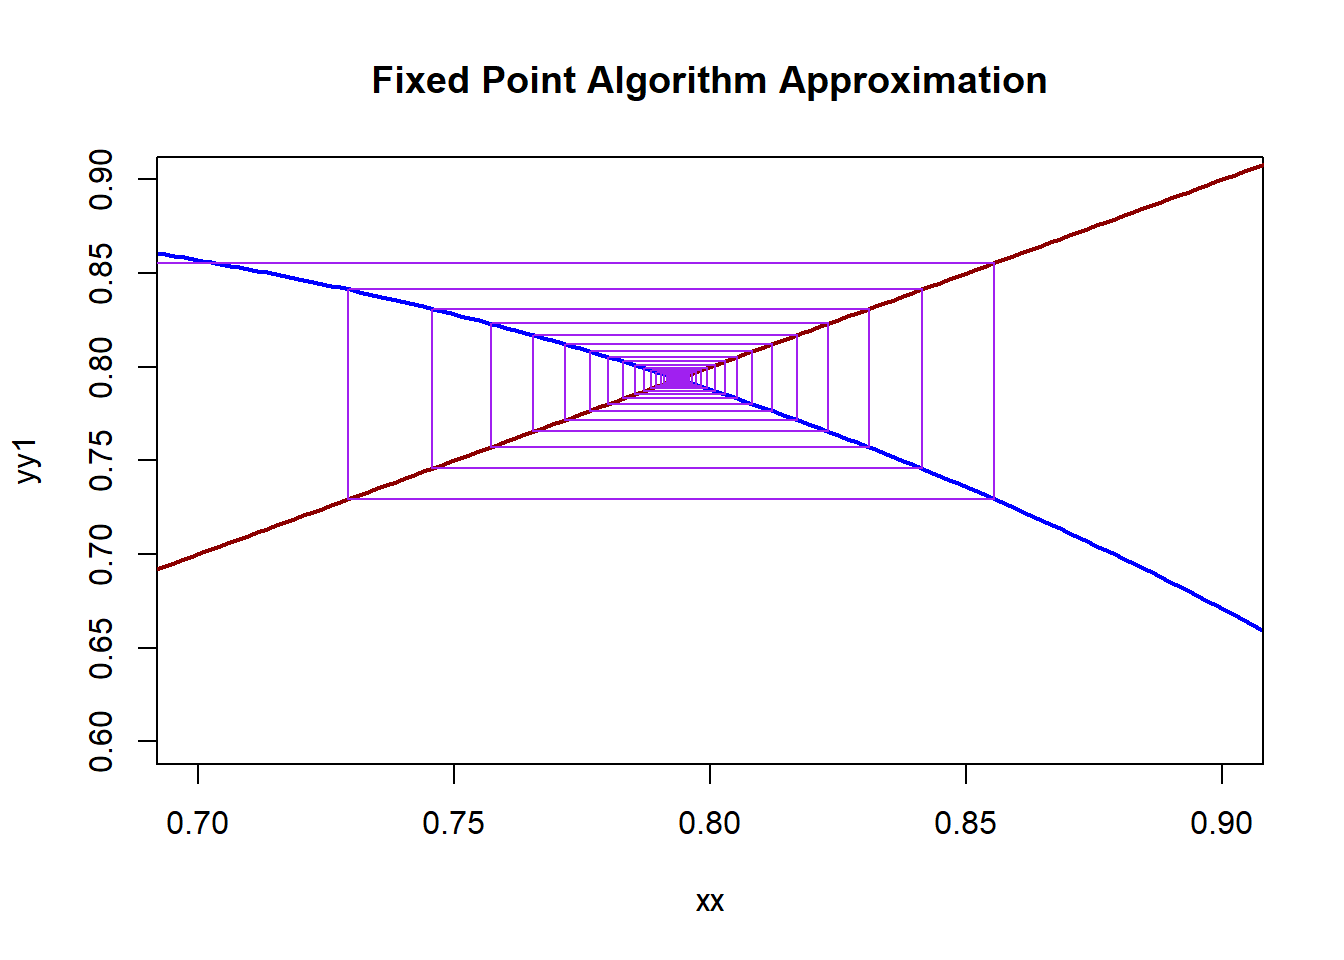
\includegraphics{MAT325EB_files/figure-latex/unnamed-chunk-49-1.pdf}

\begin{verbatim}
## 
## 
## The algorithm converges!
## The approximate root is: 0.7937047 .
## The absolute error is: 8.942928e-06 .
## The number of iterations is: 85 .
\end{verbatim}

\hypertarget{basics-of-data-representation-and-error-analysis}{%
\chapter{Basics of Data Representation and Error Analysis}\label{basics-of-data-representation-and-error-analysis}}

This note introduces briefly the concepts of floating point and the basics of error analysis. Before presenting these concepts, we introduce some computer architecture concepts from computer science.

\textbf{Bit} is the fundamental unit of memory inside a computer, which is short for \textbf{\color{red} binary digit}. \textbf{Each bit} of data corresponds to a `0' or `1'.

The bit is the smallest unit of data that a computer processes, but a single bit are too small to represent much data.

\textbf{\color{red}The smallest practical unit for expressing information is the byte, which is made up of eight bits}.

\textbf{A single byte} consists of \textbf{eight bits}. That is, a single byte can represent 256 (\(=2^8\)) combinations of data.

\hypertarget{data-representation}{%
\section{Data Representation}\label{data-representation}}

Data is a broad concept. All recorded information is called data. We briefly describe how data is represented and stored in computer systems. In this numerical analysis class, we focus on how numbers are represented and stored in computers.

\hypertarget{number-systems}{%
\subsection{Number Systems}\label{number-systems}}

We use a decimal system (base 10) for counting and computations. Computers use binary (base 2) number systems, as they are made from binary digital components (known as transistors) operating in two states - on (encoded as \(1\)) and off (encoded as \(0\)). In computing, the hexadecimal (base 16) or octal (base 8) number systems are also used as a compact form for representing binary numbers. Next, we briefly outline decimal, binary, and hexadecimal number systems. Every representation has three components: \textbf{\color{red}digits}, \textbf{\color{red}base}, and \textbf{\color{red}exponent}.

\hypertarget{decimal-base-10-system}{%
\subsubsection{Decimal (Base 10) System}\label{decimal-base-10-system}}

The decimal number system has ten symbols: \(0, 1, 2, 3, 4, 5, 6, 7, 8\), and \(9\), called \textbf{digits}. It uses positional notation. That is, the least-significant digit (right-most digit) is of the order of \(10^0\) (units or ones), the second right-most digit is of the order of \(10^1\) (tens), the third right-most digit is of the order of \(10^2\) (hundreds), and so on. The exponents of the base are called \textbf{positional numbers}.

\hfill\break

\textbf{Example 1}: The base 10 representation of integer 182736 is given the following form \[
182736 = 1\times 10^5 + 8\times 10^4 + 2\times 10^3 + 7\times 10^2 + 3\times 10^1 + 6\times 10^0.
\] The following figure explains the above representation.

\begin{center}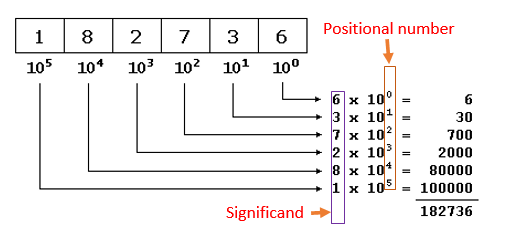
\includegraphics[width=0.85\linewidth]{img02/w02-base10Rep} \end{center}

To avoid confusion, we use \(182736D\) or \(182736_{10}\) to denote \(182736\) to be a decimal number in case multiple number systems are used at the same time.

\hfill\break

\hypertarget{binary-base-2-system}{%
\subsubsection{Binary (base 2) System}\label{binary-base-2-system}}

The binary number system is used by all computers. The binary number system is a base-2 number system, therefore there are two valid digits: 0 and 1. The binary number system has two symbols: 0 and 1, called bits. It is also a positional notation.

\textbf{Example 2}: Write the base 2 representation of binary integer 101010B.

\textbf{Solution} The base 2 representation is given in the following. \[
101010B = 1\times 2^5 + 0\times 2^4 + 1\times 2^3 + 0\times 2^2 + 1\times 2^1 + 0\times 2^0
\]

where suffix \(B\) denotes the binary number. The following figure explains the above representation.

\begin{center}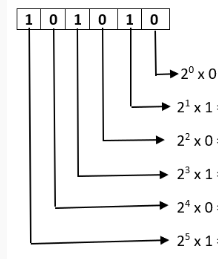
\includegraphics[width=0.35\linewidth]{img02/w02-base2Rep} \end{center}

\hfill\break

\hypertarget{conversion-between-number-systems}{%
\subsubsection{Conversion Between Number Systems}\label{conversion-between-number-systems}}

Computers use the binary system to store numbers. How to convert a number from one system to the other? The following examples illustrate the idea of conversion.

\textbf{Example 3} Convert 12045D to a binary number.

\textbf{Solution}: All we need to so is to represent 205D in a power series with base 2 in the following \[
205D = 2^7D + 2^6D + 2^3D + 2^2D + 1D  
\] \[
= 1 \times 2^7D + 1\times 2^6D +0\times 2^5D + 0\times 2^4D + 1\times 2^3D + 1\times 2^2D + 0\times 2^1D + 1\times 2^0D = 11001101B
\]\\

\textbf{Example 4}: Convert 101011B into a decimal system.

\textbf{Solution}: Use the same idea in the previous example to complete the conversion. \[
101011B = 1\times 2^5D + 0\times 2^4D + 1\times 2^3D + 0\times 2^2D + 1\times 2^1D + 1\times 2^0 
\] \[
=32D + 0D + 8D + 0D + 2D + 1D = 43D.
\]

\hfill\break

\textbf{Example 5}: Express 3.25D (floating value) into a binary (floating) value.

\textbf{Solution}: We represent the integral and decimal parts into binary numbers respectively.

\begin{itemize}
\item
  \textbf{Integral part}: \(3_{10} = (1\times 2^1 + 1\times 2^0)_{10} = (11)_2\).
\item
  \textbf{Decimal part}: \(.25_{10} = (0\times 2^{-1} + 1\times 2^{-2} = (.01)_2\).
\end{itemize}

Therefore, \(3.25_{10} = 11.01_2\).

\hfill\break

\textbf{Comment}: converting the fractional part to binary (base 2 representation) is a little cumbersome. The following is a programmatically convenient tabular algorithm:

\begin{center}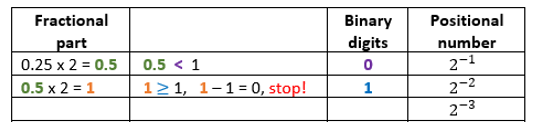
\includegraphics[width=0.75\linewidth]{img02/w02-TabularConversionBase2Fraction} \end{center}

\hfill\break

\textbf{Example 6} Express 21.36D (decimal representation) into a binary (representation) value.

\textbf{Solution}: We still convert the integral and fraction parts separately.

\begin{itemize}
\item
  \textbf{Integral Part}: \(21 = 1\times 2^4 + 0\times 2^3 + 1\times 2^2 + 0\times 2^1 + 1 \times 2^0 = (10101)_2\).
\item
  \textbf{Fractional Part}: The binary conversion of \(0.36\) is based on the following table.
\end{itemize}

\begin{center}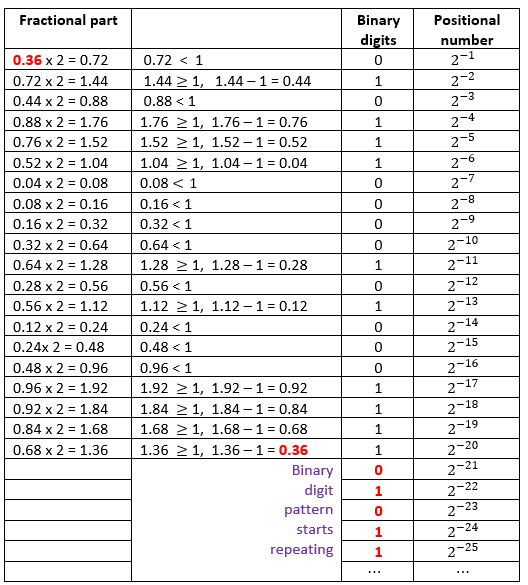
\includegraphics[width=0.95\linewidth]{img02/w02-TabularRecursiveConversionBase2Fraction} \end{center}

From the table we have \[
0.36_{10} = (\overbrace{01011100001010001111}^\text{20 digits} \cdots\overbrace{ 01011100001010001111}^\text{20 digits} \cdots)_2
\] That is, the resultant binary number has infinite digits because the sequence of digits (\(01011100001010001111\)) will repeat infinitely many times.

Therefore, \(21.36_{10} = 10101.\overline{01011100001010001111}_2\).

\textbf{Remark}: This examples shows that \(0.36\) has infinite representations in binary. The bits go on forever; no matter how many of those bits you store in a computer, you will never end up with the binary equivalent of decimal \(0.36\).

\hypertarget{scientific-notation}{%
\subsubsection{Scientific Notation}\label{scientific-notation}}

We have outlined the base-10 and base-2 representation of given numbers. We also use \textbf{scientific notation} in base-10 representation.

\textbf{Example 7}: Write the scientific notation of \(21.36_{10}\) and its binary representation (see the second part of example 6).

\textbf{Solution}: The scientific notation of \(21.36_{10}\) denoted by \(21.36 = 2.136\times 10^{1}\) or written as \(2.136E1\). In binary representation, \(21.36_{10} = 10101.\overline{01011100001010001111}_2 = 1.0101\overline{01011100001010001111}_2\times 2^4\)

\hypertarget{how-data-is-stored-in-computer-memory}{%
\section{How data is stored in computer memory}\label{how-data-is-stored-in-computer-memory}}

Human beings use decimal (base 10) and duodecimal (base 12) number systems for counting and measurements (probably because we have 10 fingers and two big toes). Computers use binary (base 2) number systems, as they are made from binary digital components (known as transistors) operating in two states - \textbf{on} and \textbf{off}.

\begin{center}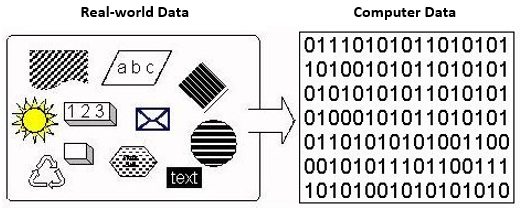
\includegraphics[width=0.65\linewidth]{img02/w02-Realworld-Computer-Data} \end{center}

We will not go into details about how all kinds of data are stored in a computer. But it is necessary to have some conceptual understanding of how numbers are stored in a computer so that we will better understand various sources of errors.

Computer memory is the collection of many groups that contain a certain number of bits. As mentioned earlier,

\begin{itemize}
\item
  a collection of 8 bits is called a byte, and
\item
  a collection of 4 bytes, or 32 bits, is called a word.
\end{itemize}

Each individual data value in a data set is usually stored using one or more bytes of memory, but at the lowest level, any data stored on a computer is just a large collection of bits. The following is an illustrative example that explains how a number is stored using a 32-bit layout (also called \textbf{bit string}) memory.

\begin{center}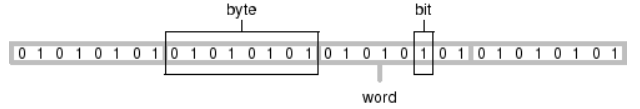
\includegraphics[width=0.85\linewidth]{img02/w02-ExampleMemoryUnit} \end{center}

\hypertarget{how-integers-are-stored-in-memory}{%
\subsection{How integers are stored in memory?}\label{how-integers-are-stored-in-memory}}

The most computer system uses 32-bit (or 64-bit) layout to store integers. The previous figure is a 32-bit string layout. The binary integer stored is \[
(\overbrace{010101010101010101010101010101010101}^\text{32 digits})_2 = (2^{30}+2^{28}+2^{26} + \cdots + 2^2 + 2^0)_{10} = 1431655765_{10}
\] If we store only unsigned integers, the biggest integer we store in the 32-bit layout is \(2^{32} - 1 = 4294967295\). The smallest integer is 0. If we consider both positive and positive integers, the use one bit (utmost left-hand side of the bit string) to denote the sign of the integer (0 indicates positive and 1 indicates negative). Then the smallest and the biggest integers that can be stored are \(-2^{31} -1 = - 2147483647\) and \(2^{31} -1 = + 2147483647\).

\hfill\break

\hypertarget{floating-point-numbers}{%
\subsection{Floating-point Numbers}\label{floating-point-numbers}}

We first describe the concepts of real numbers and floating-point numbers.

\begin{itemize}
\item
  \textbf{Floating-point numbers} are any numbers with a decimal point in them. For example, 3.14159 is a floating-point number.
\item
  \textbf{A real number} is the ``analog'' version of a floating-point number -- It \textbf{has infinite precision} and \textbf{is continuous}.
\item
  The \textbf{difference} between \emph{reals} and \emph{floating-point numbers} is that the latter has limited precision -- it really depends on the abilities of the computer. \textbf{Floating-point numbers are essentially approximations of real numbers}.
\end{itemize}

\textbf{Example 8}: Let's binary representation and floating-point representation of real number \(0.1_{10}\).

\textbf{Answer}: Using the same method used in \textbf{example 7} to represent \(0.1_{10}\), we have \[
0.1_{10} = 0.0\underbrace{\overline{0011}_2}_\text{4 digits}
\] It has infinite representation in binary representation. When it is stored in a computer system, only finite binary digits are used due to the precision of the computer.

\textbf{Example 9}: Find the difference \(3_{10}\times0.1_{10} - 0.3_{10}\).

\textbf{Answer}: The difference is 0 if calculated manually. We have shown that \(0.1_{10}\) has an infinite binary representation. However, \(0.3_{10} = (0.01001100110)_2\). When calculating the above difference in a computer, it will give a non-zero number. The result from \textbf{R} in the following

\begin{Shaded}
\begin{Highlighting}[]
\DecValTok{3}\SpecialCharTok{*}\FloatTok{0.1} \SpecialCharTok{{-}} \FloatTok{0.3}
\end{Highlighting}
\end{Shaded}

\begin{verbatim}
## [1] 5.551115e-17
\end{verbatim}

\hypertarget{how-floating-point-numbers-are-stored-in-memory}{%
\subsection{How Floating-point Numbers Are Stored in Memory?}\label{how-floating-point-numbers-are-stored-in-memory}}

IEEE 754-1985 represents numbers in binary, providing definitions for four levels of precision, of which the two most commonly used are single (32-bit) and double precision (64-bit) layouts.

\begin{center}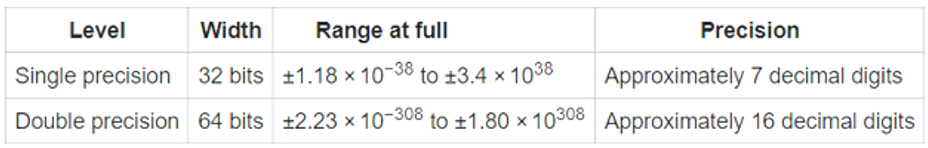
\includegraphics[width=0.85\linewidth]{img02/w02-32bit64bitPattern} \end{center}

The equation for converting a 32-bit pattern into a floating point number is given by

\[
(-1)^S\times M \times 2^{E-127}
\] where \(S\) is the value of the \emph{sign bit}, \(M\) is the value of the \emph{mantissa} (fractional part), and \(E\) is the value of component. In 32-bit layout, 23 bits are allocated to \emph{mantissa}. The general form of \(M\) is explicitly by \[
M_{10} = 1 + m_{22}2^{-1} + m_{21}2^{-2} + m_{20}2^{-3}+\cdots +m_{1}2^{-22}
\] where \(m_i\) (\(i =0, 1, 2, \cdots, 22\) is either 1 or 0. Note that \(-127\) in the conversion formula reflects the total number of alternatives based on the allocated 8 bits (\(2^8 -1 = 127\)).

The examples given below show how \(\pm 10.75_{10}\) are stored in a 32-bit layout system.

\begin{center}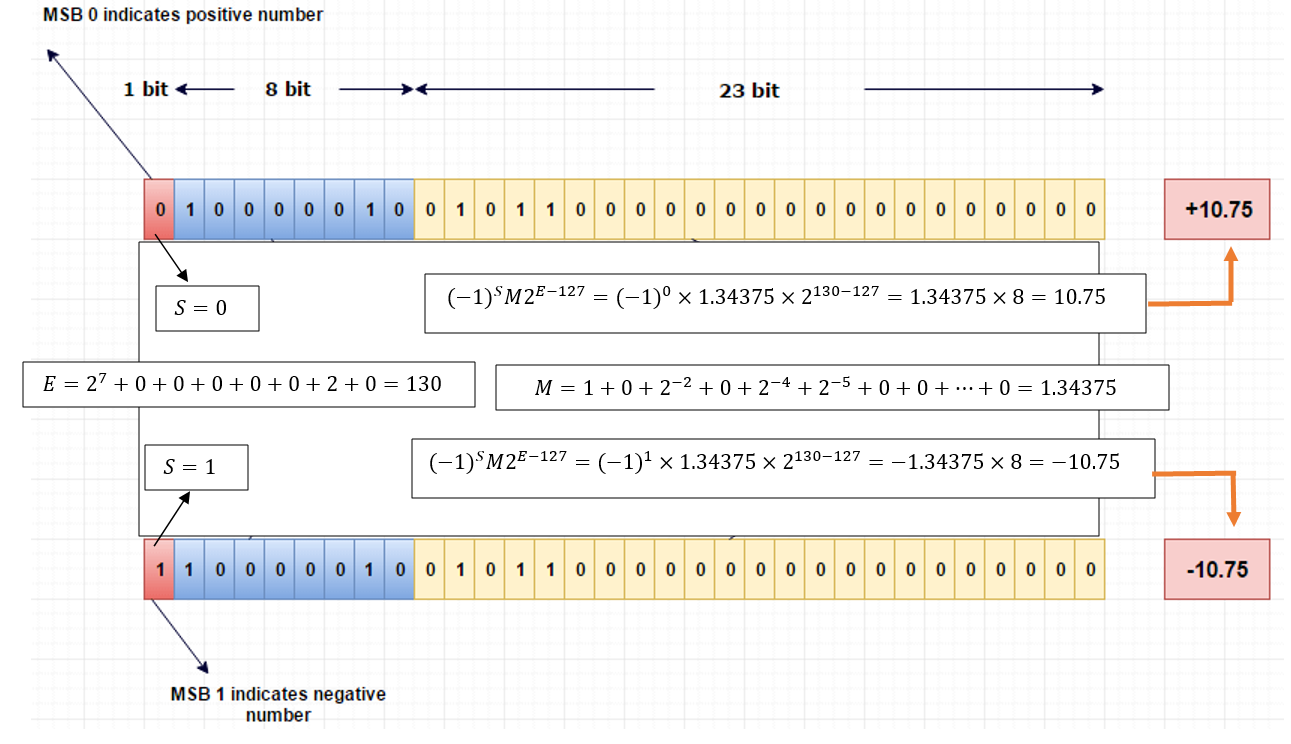
\includegraphics[width=0.95\linewidth]{img02/w02-32bitPattern} \end{center}

Of the 64 bits used to store a double precision number, bits 0 through 51 are the \emph{mantissa}, bits 52 through 62 are the \emph{exponent}, and bit 63 is the \emph{sign} bit.

\textbf{The main take-away is that storing real number to a computer system involves potential rounding error (due to approximation)!}

\hypertarget{basic-types-errors-in-error-analysis}{%
\subsection{Basic Types Errors in Error Analysis}\label{basic-types-errors-in-error-analysis}}

Let \(P\) is the true value and \(P^*\) an approximated value. Three types of errors will be used from time to time throughout the semester.

\begin{itemize}
\item
  The \textbf{actual error} is defined to be \(P-P^*\).
\item
  The \textbf{absolute error} is defined to be \(|P-P^*|\)
\item
  The \textbf{relative error} is defined to be \(|P-P^*|/P\), \(p \ne 0\). The relative errors are frequently used in error analysis throughout this semester.
\item
  \textbf{Significant digit}:
\end{itemize}

The number \(P^*\) is said to approximate \(P\) to \(t\) \textbf{significant digits} if \(t\) is the largest non-negative number such that \[
\frac{|P-P^*|}{P} < 1.23\times 10^{-t}
\]

\hypertarget{error-analysis-algorithms-and-convergence}{%
\chapter{Error Analysis, Algorithms and Convergence}\label{error-analysis-algorithms-and-convergence}}

We briefly introduce sources of errors in numerical analysis and concepts of convergence of algorithms.

\hypertarget{error-analysis}{%
\section{Error Analysis}\label{error-analysis}}

We briefly outline the sources and types of errors.

\hypertarget{understanding-numerical-error}{%
\subsection{Understanding Numerical Error}\label{understanding-numerical-error}}

We have seen that every computerized representation of real numbers with fractional parts is forced to employ rounding and other approximations. Rounding, however, represents one of many sources of error in numerical systems.

\textbf{Rounding or truncation} error comes from rounding and other approximations used to deal with the fact that we can only represent a finite set of values using most computational number systems. ** For example,**, it is impossible to write \(\pi\) exactly as an IEEE 754 floating-point value, so in practice, its value is truncated after a finite number of digits.

\textbf{Discretization} error comes from our computerized adaptations of calculus, physics,
and other aspects of continuous mathematics. \textbf{For example}, a numerical system might
attempt to approximate the derivative of a function \(f(t)\) using divided differences:
\[
f^\prime(t) \approx \frac{f(t+\epsilon) - f(t)}{\epsilon}
\]
for some fixed choice of \(\epsilon\). We must use a finite \(\epsilon > 0\) rather than taking a
limit as \(\epsilon → 0\), the resulting value for \(f^\prime(t)\) is only accurate to some number of digits. This results in a discretization error.

\textbf{Modeling} These errors arise during the modeling process when scientists ignore effecting factors in the model to simplify the problem. Also, these errors are known as formulation errors.

\hypertarget{error-classification}{%
\subsection{Error Classification}\label{error-classification}}

Let \(P = 1.354595\) is the true value and \(P^* = 1.354675\) an approximated value. Three types of errors will be used from time to time throughout the semester.

\begin{itemize}
\item
  The \textbf{actual error} is defined to be \(P-P^* = 1.354595-1.354675 = -0.00008 = -8 \cdot 10^{-5}\).
\item
  The \textbf{absolute error} is defined to be \(|P-P^*| = |1.354595 - 1.354675| = 0.00008 = 8 \cdot 10^{-5}\)
\item
  The \textbf{relative error} is generally defined to be \(|P-P^*|/P\), \(p \ne 0\). With the given values of \(P\) and \(P^*\), we have
\end{itemize}

\[
\frac{|P-P^*|}{|P|} = \frac{|1.354595 - 1.354675|}{|1.354595|} = 5.905475\times 10^{-05}
\]

The relative errors are frequently used in error analysis throughout this semester.

\hypertarget{approximation-significant-digits-figures}{%
\subsection{Approximation Significant Digits (Figures)}\label{approximation-significant-digits-figures}}

The number \(P^*\) is said to approximate \(P\) to \(t\) \textbf{significant digits} if \(t\) is the \textbf{\color{red}largest non-negative number} such that

\[
\frac{|P-P^*|}{|P|} < 5\times 10^{-t}
\]

\textbf{Example 1}: We still use \(P = 1.354595\) as the true value and \(P^* = 1.354675\) an approximated value. We have calculated

\[
\frac{|P-P^*|}{|P|} = \frac{|1.354595-1.354675|}{|1.354595|} = 5.905475\times 10^{-05}
\]

Since \(5\times 10^{-05} < 5.905475\times 10^{-05} < 5\times 10^{-04}\). Therefore, by the definition, the approximation significant digit is 4.

\textbf{Example 2} (refer to \emph{Example 5} of the textbook, page 25.) Let \(p=0.54617\) and \(q=0.54601\). Use four-digit arithmetic to approximate \(p - q\) and determine the absolute and relative errors using (a) rounding and (b) chopping.

\textbf{Solution}: The exact value of \(r = p - q\) is \(r = 0.00016\).

(a): Suppose the subtraction is performed using four-digit rounding arithmetic. Rounding p and q to four digits gives \(p^* = 0.5462\) and \(q^* = 0.5460\), respectively, and \(r^* p^* - q^* = 0.0002\) is the four-digit approximation to r. Since
\[
\frac{|r - r^*|}{|r|} = \frac{|0.00016 - 0.0002|}{|0.00016|} = 0.25 = 2.5\times 10^{-1} < 5\times 10^{-1}.
\]

By the definition, the result has only \textbf{\color{red}one significant digit}, whereas \(p^*\) and \(q^*\) were accurate to four and five significant digits, respectively.

(b). If chopping is used to obtain the four digits, the four-digit approximations to \(p\), \(q\), and \(r\) are \(p^* = 0.5461\), \(q^* = 0.5460\), and \(r^* = p^* - q^* = 0.0001\). This gives

\[
\frac{|r - r^*|}{|r|} = \frac{|0.00016 - 0.0001|}{|0.00016|} = 0.375 = 3.75\times 10^{-1} < 5\times 10^{-1}.
\]
which also results in only one significant digit of accuracy.

\hypertarget{nested-arithmetic}{%
\subsection{Nested Arithmetic}\label{nested-arithmetic}}

Accuracy loss \textbf{due to round-off error} can also be reduced by rearranging calculations, as shown in the next example.

\textbf{Example 3}: {[}examples 6 and 7 of the textbook, pages 25-27 {]}. Consider polynomial \(f(x) = x^3 - 6.1x^2 + 3.2x + 1.5\). Evaluate \(f(x)\) at = \(x = 4.71\) using three-digit arithmetic.

\textbf{Solution}: We calculate approximations

\begin{itemize}
\item
  Exact value: \(f(x) = 4.71^3 - 6.1\times 4.71^2 + 3.2\times 4.71 + 1.5 = -14.263899\)
\item
  Rounding term-wise: \(f(x) = 104 - 135 + 15.1 + 1.5 = -14.4\)
\item
  Nest rounding: \(f(x) = ((4.71 - 6.1)\times 4.71 + 3.2)\times 4.71 + 1.5=(-6.54+3.2)\times4.71+1.5 = -15.7+1.5 = 14.2\).
\end{itemize}

The above evaluation can be done using the following R code.

\begin{Shaded}
\begin{Highlighting}[]
\NormalTok{x }\OtherTok{=} \FloatTok{4.71}
\NormalTok{f.exact }\OtherTok{=}\NormalTok{ x}\SpecialCharTok{\^{}}\DecValTok{3} \SpecialCharTok{{-}} \FloatTok{6.1}\SpecialCharTok{*}\NormalTok{ x}\SpecialCharTok{\^{}}\DecValTok{2} \SpecialCharTok{+} \FloatTok{3.2}\SpecialCharTok{*}\NormalTok{x }\SpecialCharTok{+} \FloatTok{1.5}
\NormalTok{f}\FloatTok{.3}\NormalTok{digit }\OtherTok{=} \FunctionTok{signif}\NormalTok{(x}\SpecialCharTok{\^{}}\DecValTok{3}\NormalTok{,}\DecValTok{3}\NormalTok{) }\SpecialCharTok{{-}} \FunctionTok{signif}\NormalTok{(}\FloatTok{6.1}\SpecialCharTok{*}\NormalTok{ x}\SpecialCharTok{\^{}}\DecValTok{2}\NormalTok{,}\DecValTok{3}\NormalTok{) }\SpecialCharTok{+} \FunctionTok{signif}\NormalTok{(}\FloatTok{3.2}\SpecialCharTok{*}\NormalTok{x,}\DecValTok{3}\NormalTok{) }\SpecialCharTok{+} \FloatTok{1.5}
\NormalTok{f}\FloatTok{.3}\NormalTok{digit.nest }\OtherTok{=} \FunctionTok{signif}\NormalTok{((}\FunctionTok{signif}\NormalTok{((x}\FloatTok{{-}6.1}\NormalTok{)}\SpecialCharTok{*}\NormalTok{x,}\DecValTok{3}\NormalTok{) }\SpecialCharTok{+} \FloatTok{3.2}\NormalTok{)}\SpecialCharTok{*}\NormalTok{x,}\DecValTok{3}\NormalTok{) }\SpecialCharTok{+} \FloatTok{1.5}
\FunctionTok{cbind}\NormalTok{(}\AttributeTok{f.exact=}\NormalTok{f.exact, }\AttributeTok{f.3digit=}\NormalTok{f}\FloatTok{.3}\NormalTok{digit, }\AttributeTok{f.3digit.nest=}\NormalTok{f}\FloatTok{.3}\NormalTok{digit.nest)}
\end{Highlighting}
\end{Shaded}

\begin{verbatim}
##       f.exact f.3digit f.3digit.nest
## [1,] -14.2639    -14.4         -14.3
\end{verbatim}

The relative errors of the two different approximations are
\[
\text{Non-nest approximation} = \frac{|-14.2639 - (-14.4)|}{|-14.2639|} \approx 0.00954157
\]

\[
\text{Nest approximation} = \frac{|-14.2639 - (-14.3)|}{|-14.2639|} \approx 0.002530865
\]
Therefore, the nested arithmetic yields less approximation error.

Polynomials should always be expressed in the nested form before performing an evaluation because this form minimizes the number of arithmetic calculations. The error in the Illustration is due to the reduction in computations from four multiplications and three additions to two multiplications and three additions. One way to reduce round-off error is to reduce the number of computations.

\hfill\break

\hypertarget{algorithms-and-convergence}{%
\section{Algorithms and Convergence}\label{algorithms-and-convergence}}

The objective of numerical analysis is to solve continuous problems using numeric approximation but accurate numeric solutions. Numerical methods (or algorithms) are used in cases where the exact solution is impossible or prohibitively expensive to calculate.

\hypertarget{algorithm-and-psuedo-code}{%
\subsection{Algorithm and Psuedo-code}\label{algorithm-and-psuedo-code}}

\textbf{An algorithm} is a procedure that describes, in an \textbf{unambiguous} manner, a \textbf{finite} sequence of steps to be performed in a specified order. The object of the algorithm is to implement a procedure to solve a problem or approximate a solution to the problem.

Pseudo-code is a programmatic description of an algorithm that does not require any strict programming language syntax or underlying technology considerations. It is a rough draft of a program. Pseudo-code summarizes a program's flow, which is something like

\begin{center}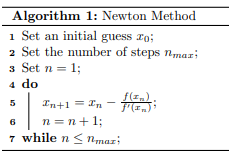
\includegraphics[width=0.3\linewidth]{img02/w02-Pseudo-Code} \end{center}

\hypertarget{rules-of-pseudo-code}{%
\subsection{Rules of Pseudo-code}\label{rules-of-pseudo-code}}

The purpose of using pseudo-code is an efficient key principle of an algorithm. It is used in planning an algorithm by sketching out the structure of the program before the actual coding takes place. The basic rules of writing pseudo-code are

\hfill\break

\textbf{Rule 1}: \emph{Write only one statement per line}

Each statement in the pseudo-code should express just one action for the computer. If the task list is properly drawn, then in most cases each task will correspond to one line of pseudo-code

\textbf{Rule 2}: \emph{Capitalize initial keyword}

There are just a few keywords we will use: \textbf{WRITE, OUTPUT, IF, ELSE, ENDIF, WHILE, ENDWHILE, REPEAT, UNTIL}

\textbf{Rule 3}: \emph{Indent to show hierarchy}

We will use a particular indentation pattern in each of the design structures:

\textbf{SEQUENCE}: keep statements that are ``stacked'' in sequence all starting in the same column.

\textbf{SELECTION}: indent the statements that fall inside the selection structure, but not the keywords that form the selection.

\textbf{LOOPING}: indent the statements that fall inside the loop, but not the keywords that form the loop.

\textbf{Rule 4}: \emph{End multi-line structures}

See how the \textbf{IF/ELSE/ENDIF} is constructed in the next example. The \textbf{ENDIF} (or END whatever) always is in line with the IF (or whatever starts the structure).

\textbf{Rule 5}: \emph{Keep statements language independent}

Pseudo-code should not be tied to any programming language. It can be implemented in any language, whether it's C++, Java, Python, MATLAB, R, or any other programming language.

\hfill\break

\textbf{Example 4}: The nth Taylor polynomial for \(f (x) = e^x\) expanded about \(x_0 = 0\) is
\[
P_n(x) =\sum_{i=0}^n \frac{x^i}{i!}
\]
and the value of \(e\) to six decimal places is 2.718282. \textbf{Construct an algorithm} to determine the \textbf{minimal value of \(n\)} required for
\[
|e - P_n(1)| < 10^{-5},
\]
without using the Taylor polynomial remainder term.

\textbf{Solution}: The objective is to determine the degrees of the Taylor polynomial evaluated at \(x = 1\) to approximate \(e\). The input values are (1) tolerance TOL and the initial degree of the Taylor polynomial. The output is the smallest degree of the Taylor polynomial that meets \(|e - P_n(1)| < TOL\).

\textbf{Caution}: In general, one should consider to include two stopping rules: error tolerance and maximum iterations. In this particular example, the maximum number of iterations is simply the solution of the problem. Therefore, there is one stopping rule: TOL

\begin{verbatim}
INPUT  initial degree: n, 
            tolerance: TOL, 
            
OUTPUT the desired degree N of the polynomial

Step 1. SET   n = 0;
            SUM = 0;  
            ERR = exp(1);
Step 2. WHILE ERR > TOL DO:
        1. SUM = SUM + 1/n!         # n! = n factorial
           ERR = exp(1) - SUM       # exp(1) = 2.718282
        2. IF |ERR| < TOL DO:
               OUTPUT (N)
               WRITE (tolerance achieved!)
               STOP
           ELSE DO:
               n = n + 1
          ENDIF
        ENDWHILE
\end{verbatim}

\hfill\break

\hypertarget{stability-of-algorithms}{%
\subsection{Stability of Algorithms}\label{stability-of-algorithms}}

Roughly speaking, the stability of an algorithm measures how good the algorithm is at solving problems to achievable accuracy. In practice, there could have several algorithms for solving one problem and some algorithms are better than others. Those algorithms that get unnecessarily inaccurate answers are called unstable.

To further consider the subject of round-off error growth and its connection to algorithm stability, suppose an error with magnitude \(E_0 > 0\) is introduced at some stage in the calculations and that the magnitude of the error after \(n\) subsequent operations is denoted by \(E_n\). The two cases that arise most often in practice are defined as follows.

\textbf{Growth of Error}: Suppose that \(E_0 > 0\) denotes an error introduced at some stage in the calculations and \(E_n\) represents the magnitude of the error after \(n\) subsequent operations.

\begin{itemize}
\item
  If \(E_n \approx CnE_0\), where \(C\) is a constant independent of \(n\), then the growth of error is said to be \textbf{linear}.
\item
  If \(En \approx C^nE_0\), for some \(C > 1\), then the growth of error is called \textbf{exponential}.
\end{itemize}

\hfill\break

\begin{center}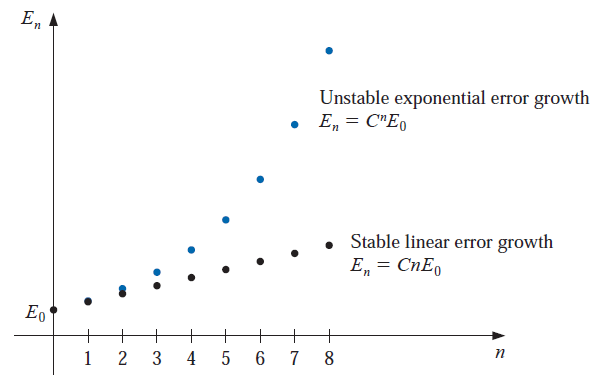
\includegraphics[width=0.6\linewidth]{img02/w02-LinearExpErrorGrowth} \end{center}

\hypertarget{rates-of-convergence}{%
\subsection{Rates of Convergence}\label{rates-of-convergence}}

Since iterative techniques involving sequences are often used, this section concludes with a brief discussion of some terminology used to describe the rate at which \textbf{convergence} occurs. In general, we would like the technique to converge as rapidly as possible. The following definition is used to compare the convergence rates of sequences.

\textbf{Convergence Sequence}: Suppose \(\{\beta_n \}_{n=1}^\infty\) is a sequence known to converge to zero, and \(\{\alpha_n \}_{n=1}^\infty\) converges to a number \(\alpha\). If a positive constant K exists with
\[
|\alpha_n - \alpha| \le K|\beta_n|, \text{ for large } n,
\]
then we say that \(\{\alpha_n \}_{n=1}^\infty\) converges to \(\alpha\) with rate, or order, of convergence \(O(\beta_n)\). (This expression is read ``big oh of \(\beta_n\)''.) It is indicated by writing \(\alpha_n = \alpha + O(\beta_n)\).

\textbf{Remark}: Since sequence, \(\{1/n^p \}_{n=1}^\infty\) (for some \(p\)) is a simple sequence, it is usually used as the base sequence to define the rate of convergence. In other words, we are interested in the largest value of \(p\) such that \(\alpha_n = \alpha + O(1/p^n)\).

\hfill\break

\textbf{Example 5}: Consider two sequences \(\{\alpha_n \}_{n=1}^\infty\) and \(\{\beta_n \}_{n=1}^\infty\) where
\[
\alpha_n = \frac{n+1}{n^2} \text{ and  } \beta_n = \frac{n + 3}{n^3}.
\]
What is the rate of convergence of the two sequences?

\textbf{Solution}: Note that
\[
\lim_{n \to \infty}\alpha_n = \lim_{n \to \infty}\frac{n+1}{n^2} = 0 \text{ and  } \lim_{n \to \infty}\beta_n = \lim_{n \to \infty}\frac{n + 3}{n^3} = 0.
\]
Therefore, \(\alpha_n = 0 + O(\frac{1}{n})\) and \(\beta_n = 0 + O(\frac{1}{n^2})\). In other words, the convergence rate of \(\{\alpha_n \}\) and \(\{ 1/n\}\) are the same, and \(\{\beta_n\}\) and \(\{1/n^2 \}\) are the same.

\hypertarget{bisection-method}{%
\chapter{Bisection Method}\label{bisection-method}}

There are different methods for root finding. The bisection method discussed in this note is useful for finding a root of single variable functions that satisfy certain assumptions.

\hypertarget{the-question}{%
\section{The Question}\label{the-question}}

\textbf{The general question to answer}: let \(f(x)\) be a single variable continuous function defined on \(D\), a sub set of \(R\). Assume there is at least one root for equation \(f(x) = 0\) on the closed interval {[}a, b{]}.

\textbf{Goal}: using a numerical method to locate the root.

Several methods can be used to find the root of a given single variable equation satisfying certain regular conditions in the next few lectures. Most of these methods are direct applications of some concepts we have already covered in elementary calculus courses.

We follow the same process throughout the semester to do numerical analysis:

\begin{itemize}
\tightlist
\item
  doing some mathematics
\item
  developing an algorithm
\item
  performing error analysis
\item
  implementing the algorithm using a programming language
\end{itemize}

\hypertarget{bisection-method-1}{%
\section{Bisection Method}\label{bisection-method-1}}

The bisection method is developed based on the \textbf{intermediate value theorem (IVT)}. If a function \(y = f(x)\) is continuous for all \(x\) in the closed interval \([a,b]\), and \(y_0\) is a number between \(f(a)\) and \(f(b)\), then there is a number \(x=c\) in \((a,b)\) that satisfies \(f(c) = y_0\).

This definition can be graphically explained in the following figure

\begin{center}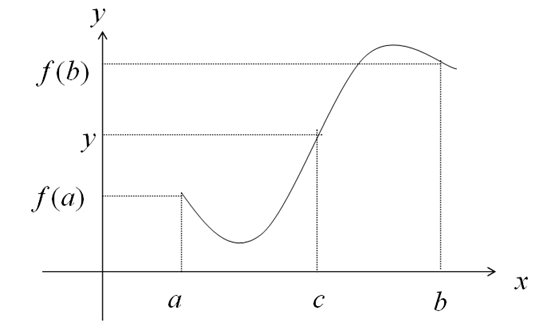
\includegraphics[width=0.45\linewidth]{img03/w03-Bisection-IVT} \end{center}

As a special case, if we have two distinct values \(x = a\) and \(x = b\) that satisfy \(f(a)f(b) < 0\). Then by the intermediate value theorem, there exists a \(c \in [a,b]\) such that \(f(c) = 0\). This means, \(f(x) = 0\) has root \(c\) in \([a, b]\).

\begin{center}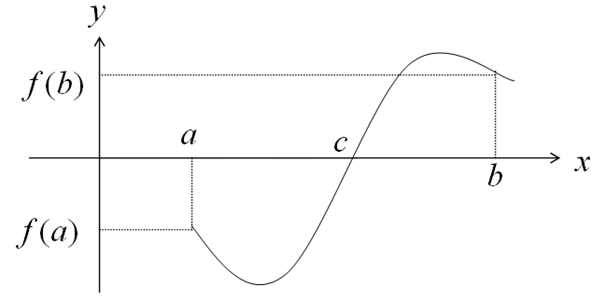
\includegraphics[width=0.45\linewidth]{img03/w03-RootExistence} \end{center}

\hypertarget{the-logic-of-bisection-method}{%
\subsection{The Logic of Bisection Method}\label{the-logic-of-bisection-method}}

The method calls for a repeated halving of sub-intervals of \([a, b]\) and, at each step, locating the half interval that contains the root \(r\) (i.e., \(f(r) = 0\)).

\url{https://github.com/pengdsci/MAT325/raw/main/w03/img/w03-bisectionMethod.gif}

\hypertarget{bisection-algorithm}{%
\subsection{Bisection Algorithm}\label{bisection-algorithm}}

Based on the logic of the bisection method, we develop the following pseudo-code to find the root of a given equation \(f(x) = 0\) on the interval \([a, b]\) assuming that \(f(a)f(b) < 0\).

\begin{verbatim}
INPUT: ending values: a, b;
           tolerance: TOL
      max. iteration: N
OUTPUT:  approximate root and errors
         error/warning messages
         intermediate outputs

STEP 1.  SET n = 0
         ERR = |b - a|
STEP 2.  WHILE ERR > TOL DO:
         STEP 3  n = n + 1               (updating iteration index)
                 SET m = a + (b - a)/2   (mid-point)
         STEP 4. IF f(m)f(b) < 0 DO:
                     a = m               (updating ending value)
                     b = b               (not necessary...)
                 ENDIF
         STEP 5. IF f(m)f(b) > 0 DO:
                    a = a
                    b = m
                 ENDIF
         STEP 6. ERR = |b - a|
                 IF ERR < TOL DO:
                     OUTPUT (p = m, other information)
                     STOP
                 ENDIF
                 IF ERR > TOL DO:
                    OUTPUT (intermediate info)
                 ENDIF
         STEP 7. IF n = N DO:
                    OUTPUT (message on iteration limit)
                    STOP
                 ENDIF
         ENDWHILE
\end{verbatim}

\hypertarget{error-analysis-1}{%
\section{Error Analysis}\label{error-analysis-1}}

Given that we have an initial bound on the problem \([a, b]\), then the maximum error of using either \(a\) or \(b\) as our approximation is \(h = b - a\). Because we halve the width of the interval with each iteration, the error is reduced by a factor of \(2\), and thus, the error after \(n\) iterations will be \(h/2^n\). Let \(r\) be the true root of \(f(x) = 0\) and \(p_n\) is the approximate root at \(n\)-th iteration. The absolute error of the bisection method is given by
\[
|r - p_n| = \frac{b - a}{2^n}.
\]
Next, we introduce the order of convergence that is defined in Section 2.4 of the textbook.

\hfill\break

\begin{center}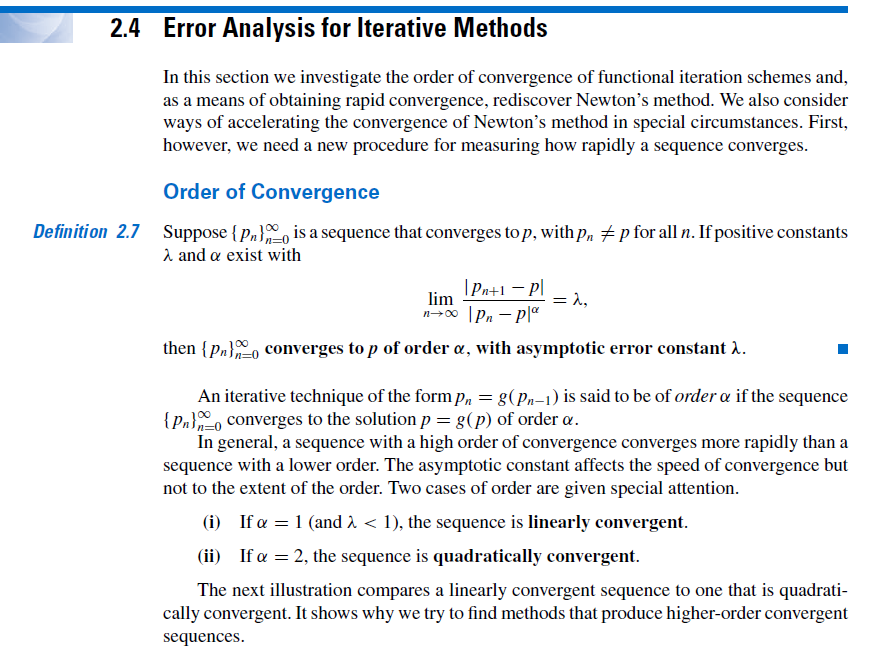
\includegraphics[width=1\linewidth]{img03/w03-ErrorAnalysis-ConvergenceOrder} \end{center}

\hfill\break

Based on the above definition of the order of convergence, we have

\[
\frac{|p_{n+1} - r|}{|p_n - r|^1} = \frac{(b-a)/2^{n+1}}{(b - a)/2^n} = \frac{1}{2}. 
\]
That is \(\alpha = 1\). Therefore, the order of convergence order of the error is \textbf{linear}.

\hfill\break

\hypertarget{numerical-examples.}{%
\section{Numerical Examples.}\label{numerical-examples.}}

We will present two examples to demonstrate the application of the bisection method.

\textbf{Example 1}: Find a root of equation \(x^3+4x^2-10 = 0\).

\textbf{Solution}: Since we are not given the interval to apply the bisection method. We first sketch \(f(x) = x^3+4x^2-10\) and \(y = 0\). The x-coordinate of the intersection of the two curves is the solution to the original equation.

\begin{Shaded}
\begin{Highlighting}[]
\NormalTok{x}\OtherTok{=} \FunctionTok{seq}\NormalTok{(}\SpecialCharTok{{-}}\DecValTok{1}\NormalTok{, }\DecValTok{2}\NormalTok{, }\AttributeTok{length =} \DecValTok{200}\NormalTok{)}
\NormalTok{y }\OtherTok{=}\NormalTok{ x}\SpecialCharTok{\^{}}\DecValTok{3}\SpecialCharTok{+}\DecValTok{4}\SpecialCharTok{*}\NormalTok{x}\SpecialCharTok{\^{}}\DecValTok{2{-}10}
\CommentTok{\#}
\FunctionTok{plot}\NormalTok{(x, y, }
     \AttributeTok{type =} \StringTok{"l"}\NormalTok{,}
     \AttributeTok{lty =} \DecValTok{1}\NormalTok{,}
     \AttributeTok{lwd =} \DecValTok{2}\NormalTok{,}
     \AttributeTok{col =} \StringTok{"blue"}\NormalTok{,}
     \AttributeTok{xlab =} \StringTok{"X"}\NormalTok{,}
     \AttributeTok{ylab =} \StringTok{"Y"}\NormalTok{,}
     \AttributeTok{main =} \StringTok{"The curve of y = x\^{}3+4x\^{}2{-}10"}\NormalTok{)}
\FunctionTok{abline}\NormalTok{(}\AttributeTok{h =} \DecValTok{0}\NormalTok{, }\AttributeTok{lty =} \DecValTok{2}\NormalTok{, }\AttributeTok{lwd =} \DecValTok{1}\NormalTok{, }\AttributeTok{col =} \StringTok{"darkred"}\NormalTok{)}
\end{Highlighting}
\end{Shaded}

\begin{center}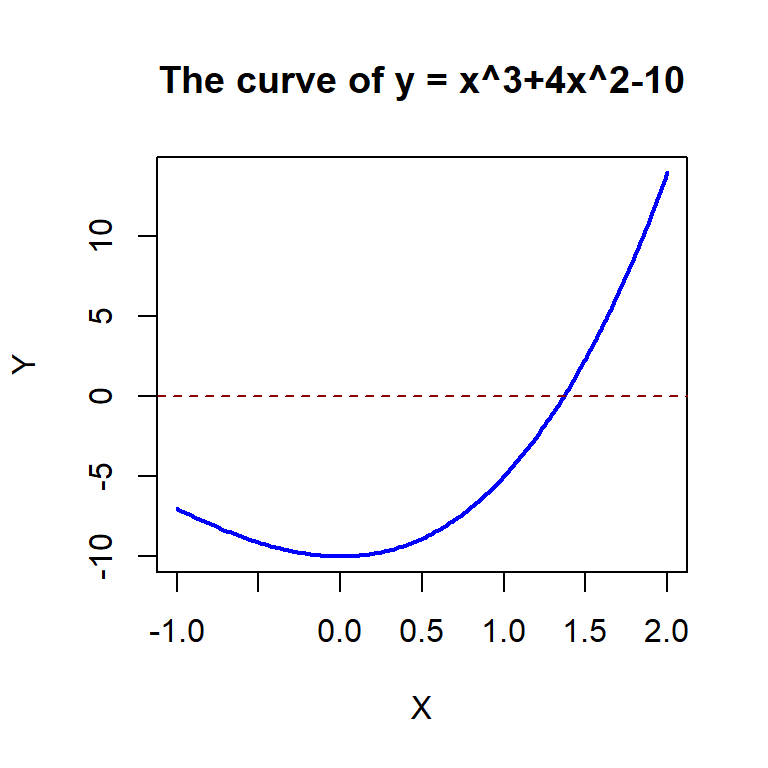
\includegraphics{MAT325EB_files/figure-latex/unnamed-chunk-66-1} \end{center}

Based on the above curve, we choose \([a, b] = [1,2]\) to implement the bisection algorithm with the following code.

\begin{Shaded}
\begin{Highlighting}[]
\DocumentationTok{\#\# we first define the R function based on the given equation}
\NormalTok{fn }\OtherTok{=} \ControlFlowTok{function}\NormalTok{(x)\{}
\NormalTok{   f.val }\OtherTok{=}\NormalTok{   x}\SpecialCharTok{\^{}}\DecValTok{3} \SpecialCharTok{+} \DecValTok{4}\SpecialCharTok{*}\NormalTok{x}\SpecialCharTok{\^{}}\DecValTok{2} \SpecialCharTok{{-}} \DecValTok{10}
\NormalTok{   f.val}
\NormalTok{\}}

\DocumentationTok{\#\# INPUT INFO}
\NormalTok{  a }\OtherTok{=} \DecValTok{0}
\NormalTok{  b }\OtherTok{=} \DecValTok{2}
\NormalTok{  TOL }\OtherTok{=} \DecValTok{10}\SpecialCharTok{\^{}}\NormalTok{(}\SpecialCharTok{{-}}\DecValTok{6}\NormalTok{)            }\CommentTok{\# tolerance limit}
\NormalTok{  N }\OtherTok{=} \DecValTok{200}                   \CommentTok{\# max iterations}
\DocumentationTok{\#\# Initialization}
\NormalTok{  n  }\OtherTok{=} \DecValTok{0}
\NormalTok{  ERR }\OtherTok{=} \FunctionTok{abs}\NormalTok{(b }\SpecialCharTok{{-}}\NormalTok{ a)}
\DocumentationTok{\#\# Loop begins}
\ControlFlowTok{while}\NormalTok{(ERR }\SpecialCharTok{\textgreater{}}\NormalTok{ TOL)\{}
\NormalTok{  n }\OtherTok{=}\NormalTok{ n }\SpecialCharTok{+} \DecValTok{1}
\NormalTok{  m }\OtherTok{=}\NormalTok{ a }\SpecialCharTok{+}\NormalTok{ (b }\SpecialCharTok{{-}}\NormalTok{ a) }\SpecialCharTok{/} \DecValTok{2}     \CommentTok{\# midpoint of interval [a, b]}
  \ControlFlowTok{if}\NormalTok{ (}\FunctionTok{fn}\NormalTok{(m)}\SpecialCharTok{*}\FunctionTok{fn}\NormalTok{(b) }\SpecialCharTok{\textless{}} \DecValTok{0}\NormalTok{)\{   }\CommentTok{\# new interval should be [m, b]}
\NormalTok{      a }\OtherTok{=}\NormalTok{ m               }\CommentTok{\# m will be the new a}
\NormalTok{      b }\OtherTok{=}\NormalTok{ b}
\NormalTok{  \} }\ControlFlowTok{else}\NormalTok{ \{                }\CommentTok{\# new interval should be [a,m]}
\NormalTok{      a }\OtherTok{=}\NormalTok{ a}
\NormalTok{      b }\OtherTok{=}\NormalTok{ m               }\CommentTok{\# m will be the new \textquotesingle{}b\textquotesingle{}}
\NormalTok{   \}}
\NormalTok{  ERR }\OtherTok{=} \FunctionTok{abs}\NormalTok{(b }\SpecialCharTok{{-}}\NormalTok{ a)        }\CommentTok{\# updated absolute error}
  \DocumentationTok{\#\# Output information}
  \ControlFlowTok{if}\NormalTok{(ERR }\SpecialCharTok{\textless{}}\NormalTok{ TOL)\{  }\CommentTok{\# if the absolute error is less than TOL, print out results}
    \FunctionTok{cat}\NormalTok{(}\StringTok{"}\SpecialCharTok{\textbackslash{}n}\StringTok{The algorithm converges!"}\NormalTok{)}
    \FunctionTok{cat}\NormalTok{(}\StringTok{"}\SpecialCharTok{\textbackslash{}n}\StringTok{The number of iteration n ="}\NormalTok{, n, }\StringTok{"."}\NormalTok{)}
    \FunctionTok{cat}\NormalTok{(}\StringTok{"}\SpecialCharTok{\textbackslash{}n}\StringTok{The approximate root r ="}\NormalTok{, (a }\SpecialCharTok{+}\NormalTok{ b)}\SpecialCharTok{/}\DecValTok{2}\NormalTok{,}\StringTok{"."}\NormalTok{)}
    \FunctionTok{cat}\NormalTok{(}\StringTok{"}\SpecialCharTok{\textbackslash{}n}\StringTok{The absolute error ERR ="}\NormalTok{, ERR,}\StringTok{"."}\NormalTok{)}
    \ControlFlowTok{break}
\NormalTok{  \} }\ControlFlowTok{else}\NormalTok{ \{            }\DocumentationTok{\#\# output of intermediate iteration}
    \FunctionTok{cat}\NormalTok{(}\StringTok{"}\SpecialCharTok{\textbackslash{}n}\StringTok{Iteration:"}\NormalTok{,n,}\StringTok{". The absolute error ERR ="}\NormalTok{, ERR, }\StringTok{"."}\NormalTok{)  }
\NormalTok{    \}}
  \DocumentationTok{\#\#\# Test attainment to the max iteration}
  \ControlFlowTok{if}\NormalTok{(n }\SpecialCharTok{==}\NormalTok{ N)\{ }
    \FunctionTok{cat}\NormalTok{(}\StringTok{"}\SpecialCharTok{\textbackslash{}n\textbackslash{}n}\StringTok{ Iteration limit reached. The algorithm diverges!"}\NormalTok{)}
    \ControlFlowTok{break}
\NormalTok{  \}}
\NormalTok{\}}
\end{Highlighting}
\end{Shaded}

\begin{verbatim}
## 
## Iteration: 1 . The absolute error ERR = 1 .
## Iteration: 2 . The absolute error ERR = 0.5 .
## Iteration: 3 . The absolute error ERR = 0.25 .
## Iteration: 4 . The absolute error ERR = 0.125 .
## Iteration: 5 . The absolute error ERR = 0.0625 .
## Iteration: 6 . The absolute error ERR = 0.03125 .
## Iteration: 7 . The absolute error ERR = 0.015625 .
## Iteration: 8 . The absolute error ERR = 0.0078125 .
## Iteration: 9 . The absolute error ERR = 0.00390625 .
## Iteration: 10 . The absolute error ERR = 0.001953125 .
## Iteration: 11 . The absolute error ERR = 0.0009765625 .
## Iteration: 12 . The absolute error ERR = 0.0004882812 .
## Iteration: 13 . The absolute error ERR = 0.0002441406 .
## Iteration: 14 . The absolute error ERR = 0.0001220703 .
## Iteration: 15 . The absolute error ERR = 6.103516e-05 .
## Iteration: 16 . The absolute error ERR = 3.051758e-05 .
## Iteration: 17 . The absolute error ERR = 1.525879e-05 .
## Iteration: 18 . The absolute error ERR = 7.629395e-06 .
## Iteration: 19 . The absolute error ERR = 3.814697e-06 .
## Iteration: 20 . The absolute error ERR = 1.907349e-06 .
## The algorithm converges!
## The number of iteration n = 21 .
## The approximate root r = 1.36523 .
## The absolute error ERR = 9.536743e-07 .
\end{verbatim}

\hypertarget{fixed-point-method}{%
\chapter{Fixed Point Method}\label{fixed-point-method}}

\hfill\break

\textbf{Goal}: Find the root of equation \(f(x) = 0\) over interval \([a, b]\).

\hfill\break

\textbf{Definition of Fixed-point Problem}: The number \(p\) is a fixed point for a given function \(g\) if \(g( p) = p\). In other words, if function \(g(x)\) has a fixed point \(p\), then \(p\) is a root of equation \(g(x) - x = 0\).

\textbf{Root-finding versus Fixed-point Problems}: we could convert root finding problem \(f(x) = 0\) to fixed-point problem \(g(x) = af(x) + x = x\) for any real number \(a \ne 0\).

This section discusses how to approximate the root \(p\) using the \textbf{Fixed-point Method}.

\hypertarget{some-theories-of-the-fixed-point-method}{%
\section{Some Theories of the Fixed Point Method}\label{some-theories-of-the-fixed-point-method}}

\textbf{Theorem 1} (Existence of fixed point)

Suppose that \(g(x)\) is a continuous function that maps its domain, \(D\), onto a subset of itself, \(S = g(D)\), i.e., \(g(x) \in C[a, b]\), such that

\[
g(x): [a,b]\to S \subset [a, b]
\]

Then \(g(x)\) has a fixed point in \([a, b]\).

\textbf{Proof}: If \(g(a) = a\) or \(g(b) = b\), we are done.

Assume \(g(a) \ne a\) and \(g(b) \ne b\). Since \(g([a,b]) \subset [a, b]\), we have \(g(a) > a\) and \(g(b) < b\). Let \(h(x) = g(x) - x\). Since \(g(x) \in C[a, b]\), so is \(h(x) \in C[a, b]\). Observe that \(h(a) = g(a) - a > 0\), \(h(b) = g(b) - b < 0\). By intermediate value theorem, there exists at least one value \(r\) in \([a, b]\) such that \(h(r) = 0\). That implies that \(g(r) = r\). This completes the proof.

\textbf{Corollary}: Every continuous bounded function on the real numbers has a fixed point.

\hfill\break

\textbf{Theorem 2} (Uniqueness of fixed point, also called Contraction Mapping Theorem)

Suppose that \(g(x)\) is a continuous function that maps its domain, \(D\), onto a subset of itself, \(S = g(D)\), i.e., \(g(x) \in C[a, b]\), such that

\[
g(x): [a,b]\to S \subset [a, b]
\]

Suppose further that there exists some positive constant \(0 < K < 1\) such that \(|g^\prime(x)| < K\) for all \(x\) in \([a, b]\). Then \(g(x)\) has a unique fixed point \(p\) in \([a, b]\).

\textbf{Proof}: Assume there at least two fixed points, say \(p_1\) and \(p_2\) in \([a,b]\), such that \(g(p_1) = p_1\) and \(g(p_2) = p_2\) with \(p_1 < p_2\). That is, \(g(p_2) - g(p_1) = p_2 - p_1\).

On the other hand, the mean value theorem indicated that \(g(p_2) - g(p_1) = g^\prime (c)(p_2 - p_1)\) for some \(c\) in \([p_1, p_2]\). Since , we have \(g(p_2) - g(p_1) < p_2 – p_1\). This \textbf{contradicts} with \(g(p_2) - g(p_1) = p_2 - p_1\). Therefore, we have proved the uniqueness of the fixed point. The proof is completed.

\hfill\break

\hypertarget{fixed-point-iteration}{%
\section{Fixed Point Iteration}\label{fixed-point-iteration}}

With the theory developed previously, we focus on the following recursive equation for finding the fixed point numerically.

Choose an initial approximation \(p_0\), generate sequence \(\{p_n\}_{n=0}^\infty\) by \(p_n = g(p_{n-1})\). If the sequence converges to \(p\) and \(g(x)\) is continuous at p, then

\[
p = \lim_{n \to \infty}p_n = \lim_{n \to \infty}g(p_{n-1}) = g(p)
\]

\begin{center}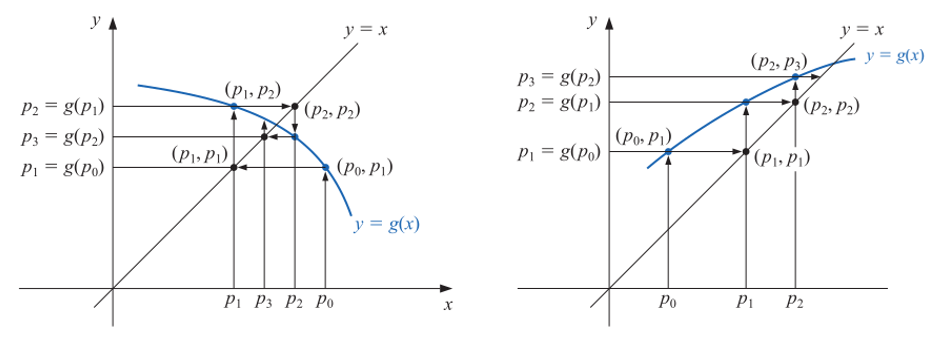
\includegraphics[width=0.8\linewidth]{img03/w03-FixedPointIteration} \end{center}

The following animated graph demonstrates the process of searching the fixed point.

\url{https://github.com/pengdsci/MAT325/raw/main/w03/img/Fixed_point_anime.gif}

\textbf{Fixed-point Iteration Algorithm}

\begin{verbatim}
INPUT    f(x), 
         initial p0, 
         TOL
         N                       (max iterations)
STEP 1.  ERR = infinity          (initial error - must be a big number)
         x                       (initial value)
         n = 0                   (initial iterator)
STEP 2.  WHILE ERR > TOL DO:
         STEP 3. n = n + 1
         STEP 4. new.x = f(x)
                 ERR = new.x - x
                 IF ERR < TOL DO:
                    OUTPUT (results)
                    STOP
                  ENDIF
                 IF ERR > TOL DO:
                   OUTPUT (intermediate results)
                   x = new.x      (update x value)
                 ENDIF
                 IF n == N DO:
                   OUTPUT ()
                   STOP
                 ENDIF
\end{verbatim}

\hfill\break

\hypertarget{error-analysis-2}{%
\section{Error Analysis}\label{error-analysis-2}}

\hfill\break

By the Lipschitz condition in the definition of \textbf{Contraction Mapping Theorem}, the approximated error is easily obtained as \(|p_{n+1} - p_n| \le K^n|p_1 – p_0|\). Next, we present a result that gives the bound the true error.

\textbf{Theorem 3} (Error Estimation)

If fixed point iteration is terminated after \(n > 1\) steps then the error is limited by

\[
|p_n-p| \le \frac{K^n|p_1-p_0|}{1-K}
\]

where \(0< K < 1\) is the Lipschitz constant.

\textbf{Proof} We use mathematical induction to prove this theorem. For \(n = 1\), we need to show that

\[
|p_1 - p| \le \frac{K}{K-1}|p_1-p_0|.
\] To this end, we use the Mean Value Theorem, there exists a constant \(c \in [\min\{p, p_0\}, \max\{p, p_0\}]\) such that

\[
|g^\prime(c)| = \left|\frac{f(p_0)-f(p)}{p_0-p} \right| = \left|\frac{p_1-p}{p_0-p} \right|\le K.
\]

That is, \(|p_1-p| \le K|p_0-p|\). Using the triangular inequality, we have

\[
|p_1 - p| \le K|p_0-p| = K|p_0 - p_1 + p_1 -p| \le K|p_1-p_0| + K|p_1-p|
\]
Therefore
\[
|p_1-p|\le\frac{K}{K-1}|p_1-p_0|.
\]

We assume that original inequality is true when \(n = m\), i.e.,

\[
|p_m-p| \le \frac{K^m|p_1-p_0|}{1-K}.
\]
We want to show that

\[
|p_{m+1}-p| \le \frac{K^{m+1}|p_1-p_0|}{1-K}.
\]

We still use the MVT on interval \([\min\{p, p_m\}, \max\{p, p_m\}]\) to get

\[
|g^\prime(c)| = \left|\frac{f(p_m)-f(p)}{p_m-p} \right| = \left|\frac{p_{m+1}-p}{p_m-p} \right|\le K.
\]
where \(c\in [\min\{p, p_m\}, \max\{p, p_m\}]\). Therefore,

\[
|p_{n+1}-p| \le K|p_n - p|
\]
and

\[
|p_{m+1} - p| \le K|p_m-p_0| = \frac{K^{m+1}}{1-K}|p_1-p_0|.
\]

This completes the proof.

\textbf{Corollary} (Order of Convergence)

If the fixed-point method converges, it has a linear convergence order.

The proof has already been given in the proof of the above theorem.

\hfill\break

\hypertarget{numerical-example-1}{%
\section{Numerical Example}\label{numerical-example-1}}

We know that there is a solution for the equation \(x^3-7x+2 = 0\) in \([0, 1]\). We rewrite the equation in the form \(x = (x^3 + 2)/7\) and denote the process \(x_{n+1} = (x^3_n + 2)/7\). We see from the following figures that if \(0 \le x_0 \le 1\) then (\(x_n\)) converges to a root of the above equation. We also note that if we start with (for example) \(x_0 = 2.5\) then the recursive process does not converge.

\begin{Shaded}
\begin{Highlighting}[]
\DocumentationTok{\#\# input values}
\NormalTok{TOL }\OtherTok{=} \DecValTok{10}\SpecialCharTok{\^{}}\NormalTok{(}\SpecialCharTok{{-}}\DecValTok{6}\NormalTok{)}
\NormalTok{  M }\OtherTok{=} \DecValTok{200}
\DocumentationTok{\#\#\#\#}
\NormalTok{gfun }\OtherTok{=} \ControlFlowTok{function}\NormalTok{(x) (x}\SpecialCharTok{\^{}}\DecValTok{3} \SpecialCharTok{+} \DecValTok{2}\NormalTok{)}\SpecialCharTok{/}\DecValTok{7}
\DocumentationTok{\#\#\#\#}
\NormalTok{ a }\OtherTok{=} \DecValTok{0}
\NormalTok{ b }\OtherTok{=} \DecValTok{2}
\NormalTok{ x }\OtherTok{=} \DecValTok{2}       \CommentTok{\# initial value of x}
\NormalTok{ n }\OtherTok{=} \DecValTok{0}        \CommentTok{\# initializing iterator}
\NormalTok{ ERR }\OtherTok{=} \ConstantTok{Inf}    \CommentTok{\# initial error}
\DocumentationTok{\#\# }
 \ControlFlowTok{while}\NormalTok{ (ERR }\SpecialCharTok{\textgreater{}}\NormalTok{ TOL)\{}
\NormalTok{  n }\OtherTok{=}\NormalTok{ n }\SpecialCharTok{+} \DecValTok{1}
\NormalTok{  new.x }\OtherTok{=} \FunctionTok{gfun}\NormalTok{(x)}
\NormalTok{  ERR }\OtherTok{=} \FunctionTok{abs}\NormalTok{(new.x }\SpecialCharTok{{-}}\NormalTok{ x)}
  \ControlFlowTok{if}\NormalTok{(ERR }\SpecialCharTok{\textless{}}\NormalTok{ TOL)\{}
    \FunctionTok{cat}\NormalTok{(}\StringTok{"}\SpecialCharTok{\textbackslash{}n\textbackslash{}n}\StringTok{The algorithm converges!"}\NormalTok{)}
    \FunctionTok{cat}\NormalTok{(}\StringTok{"}\SpecialCharTok{\textbackslash{}n}\StringTok{The approximate root is:"}\NormalTok{, new.x,}\StringTok{"."}\NormalTok{)}
    \FunctionTok{cat}\NormalTok{(}\StringTok{"}\SpecialCharTok{\textbackslash{}n}\StringTok{The absolute error is:"}\NormalTok{, ERR, }\StringTok{"."}\NormalTok{)}
    \FunctionTok{cat}\NormalTok{(}\StringTok{"}\SpecialCharTok{\textbackslash{}n}\StringTok{The number of iterations is:"}\NormalTok{, n, }\StringTok{"."}\NormalTok{)}
    \ControlFlowTok{break}
\NormalTok{  \} }\ControlFlowTok{else}\NormalTok{\{}
    \ControlFlowTok{if}\NormalTok{(ERR }\SpecialCharTok{\textgreater{}} \DecValTok{10}\SpecialCharTok{\^{}}\DecValTok{7}\NormalTok{)\{}
        \FunctionTok{cat}\NormalTok{(}\StringTok{"}\SpecialCharTok{\textbackslash{}n\textbackslash{}n}\StringTok{The algorithm diverges!"}\NormalTok{)}
        \ControlFlowTok{break}
\NormalTok{    \} }\ControlFlowTok{else}\NormalTok{\{}
         \FunctionTok{cat}\NormalTok{(}\StringTok{"}\SpecialCharTok{\textbackslash{}n}\StringTok{Iteration:"}\NormalTok{,n,}\StringTok{". Estimated root:"}\NormalTok{, new.x, }\StringTok{". Absolute error:"}\NormalTok{, ERR,}\StringTok{"."}\NormalTok{)}
\NormalTok{         x }\OtherTok{=}\NormalTok{ new.x              }\CommentTok{\# update x value!!!}
\NormalTok{    \}}
\NormalTok{  \}}
  \ControlFlowTok{if}\NormalTok{(n }\SpecialCharTok{==}\NormalTok{ M)\{}
    \FunctionTok{cat}\NormalTok{(}\StringTok{"}\SpecialCharTok{\textbackslash{}n\textbackslash{}n}\StringTok{The maximum number of iterations is achieved!"}\NormalTok{)}
    \ControlFlowTok{break}
\NormalTok{  \} }
\NormalTok{ \}}
\end{Highlighting}
\end{Shaded}

\begin{verbatim}
## 
## Iteration: 1 . Estimated root: 1.428571 . Absolute error: 0.5714286 .
## Iteration: 2 . Estimated root: 0.7022074 . Absolute error: 0.726364 .
## Iteration: 3 . Estimated root: 0.3351793 . Absolute error: 0.3670281 .
## Iteration: 4 . Estimated root: 0.2910937 . Absolute error: 0.04408562 .
## Iteration: 5 . Estimated root: 0.289238 . Absolute error: 0.001855685 .
## Iteration: 6 . Estimated root: 0.289171 . Absolute error: 6.696095e-05 .
## Iteration: 7 . Estimated root: 0.2891686 . Absolute error: 2.400242e-06 .
## 
## The algorithm converges!
## The approximate root is: 0.2891685 .
## The absolute error is: 8.601697e-08 .
## The number of iterations is: 8 .
\end{verbatim}

\hypertarget{newtons-method}{%
\chapter{Newton's Method}\label{newtons-method}}

We have introduced bisection and fixed-point methods for finding the root of single-variable equations over a pre-selected interval. Both methods have a linear convergence rate (if the error sequence converges). This note introduces the well-known Newton method for finding the root of non-linear equations. We will see that the Newton method has a quadratic convergence rate (if converges). Unlike the bisection method, this method can be extended to multi-variable nonlinear systems (same as the fixed-point method).

\hypertarget{notations-big-o-and-little-o}{%
\section{Notations: Big O and Little o}\label{notations-big-o-and-little-o}}

We have introduced the concept of convergence rate at which some function changes as its argument grows (or shrinks), without worrying too much about the detailed form. This is what the O(·) and o(·) notation are. We now give a little more detail about these notations.

A function \(f (n)\) is ``of constant order'', or ``of order 1'' when there exists some non-zero constant c such that
\[
\frac{f (n)}{c} \to 1
\]
as \(n \to 1\); equivalently, since \(c\) is a constant, \(f (n)\to c\) as \(n \to 1\). It doesn't matter how big or how small \(c\) is, just so long as there is some such constant. We then write

\[
f(n) = O(1)
\]
and say that ``the proportionality constant c gets absorbed into the big O''. For
example, if \(f (n) = 37\), then \(f (n) = O(1)\). But if \(g (n) = 37(1 -2/n)\), then \(g(n) = O(1)\)

The other orders are defined recursively. Saying
\[
g(n) = O(f(n))
\]
means
\[
\frac{g(n)}{f(n)} = O(1), \text{ or }  \frac{g(n)}{f(n)} \to c,
\]
as \(n \to \infty\). This is equivalently to say that \(g(n)\) is \textbf{of the same order} as \(f(n)\), and they \textbf{grow at the same rate}!

\hfill\break
\textbf{Example 1}: a quadratic function \(a_1n^2 + a_2n + a_3 = O(n^2)\), no matter what the coefficients are. On the other hand, \(b_1n^{-2} + b_1n^{-1} is O(n^-1)\).

Big-O means ``is of the same order as''. The corresponding little-o means ``is ultimately smaller than'': \(f (n) = o(1)\) means that \(f (n)/c \in 0\) for any constant \(c\). Reccursively, \(g (n) = o(f (n))\) means \(g (n)/ f (n) = o(1)\), or \(g (n)/ f (n) \to 0\). We also read \(g (n) = o(f (n))\) as ``\(g (n)\) is ultimately negligible compared to \(f (n)\)''.

\hfill\break

\hypertarget{foundations-of-newton-method}{%
\section{Foundations of Newton Method}\label{foundations-of-newton-method}}

\textbf{The Newton method is formulated based on the Taylor series.}

\hypertarget{the-algorithmic-logic}{%
\subsection{The Algorithmic Logic}\label{the-algorithmic-logic}}

Let's consider a general function \(f(x)\). For the starting point \(x_0\), the slope of the tangent line at the point \((x_0,f(x_0))\) is \(f\prime(x_0)\) so the equation of the tangent line is \(y-f(x_0)=f\prime(x_0)(x-x_0)\). We look at the intersection between the tangent line and \(x\)-axis: \((x_1, 0)\)

\begin{center}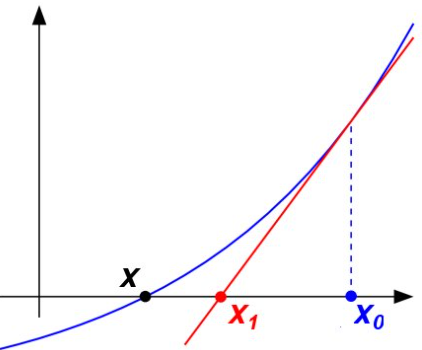
\includegraphics[width=0.4\linewidth]{img04/w04-NewtonInitialStep} \end{center}

where \(x_1\) is the root of \(0-f(x_0)=f^\prime(x_0)(x-x_0)\). solving the equation, we have \(x_1= x_0 - f(x_0)/f^\prime(x_0)\). In the above figure, we can see \(x_1\) is closer to the true root \(x\). If we draw the tangent line at \((x_1, f(x_1))\) and look at the intersection between the x-axis and this tangent line, the x-coordinate \(x_2 = x_1 - f(x_1)/f^\prime(x_1)\).

\url{https://github.com/pengdsci/MAT325/raw/main/w04/img/w04-NewtonIterationGIF.gif}

Starting with \(x_1\) and repeating this process we have \(x_2 = x_1 - f(x_1)/f^\prime (x_1)\), we get \(x_3=x_2-f(x_2)/f^\prime(x_2)\); and so on.

\hfill\break

\hypertarget{initial-starting-value-matters}{%
\subsection{Initial Starting Value Matters}\label{initial-starting-value-matters}}

Here are a few examples with different starting values. We can see the number of iterations needed to achieve the error tolerance.

\textbf{Example 2}. Find the root of equation \(f(x) = x^3 - x + 3 = 0\) using various initial starting values.

\textbf{Case 1}: \(x_0 = -1\). The algorithm converges after 6 iterations.

\textbf{Case 2}: \(x_0 = -0.1\). The algorithm converges after 33 iterations.

\textbf{Case 3}: \(x_0 = 0\). The algorithm \textbf{diverges} with the initial value \(x_0 = 0\)!

\hfill\break

\hypertarget{algorithm-and-pseudo-code}{%
\section{Algorithm and Pseudo-code}\label{algorithm-and-pseudo-code}}

Assume that \(f(x)\in C^2[a,b]\). Let \(x_0 \in [a, b]\) be an approximation to \(p\), \textbf{the root of \(f(x) = 0\)}, such that \(f(x_0) \ne 0\) and \(|p-x_0|\) is ``small.''

Consider the first Taylor polynomial for \(f(x)\) expanded about \(x_0\) and evaluated at \(x = p\).
\[
f(p) = f(x_0) + (p - x_0)f^\prime(x_0) + \frac{(p - x_0)^2}{2}f^{\prime\prime}(\xi(p))
\]
where \(\xi(p)\) is some number in \([\min{x_0, p}, \max{p, x_0}]\). Since \(f(p) = 0\) and \(|p-x_0|\) is ``small'', therefore, \(0 \approx f(x_0) - (p - x_0)f^\prime(x_0)\). This yields
\[
p \approx x_0 -\frac{f(x_0)}{f^\prime(x_0)} \to x_1
\]

As demonstrated in the previous section, continuing this process, we have \(\{x_n\}_{n = 0}^\infty\), where
\[
x_{n+1} = x_n - \frac{f(x_n)}{f^\prime(x_n)} \text{ for } n \ge 0,
\]

to approximate the root of equation \(f(x) = 0\).

\textbf{Pseudo-code of Newton Method}:

\begin{verbatim}
INPUT:   initial x0;
         TOL;
         M = maximum iterations.
         f(x)
         f'(x)
OUTPUT:  Approximated root and optional information.

STEP 1:  n = 0    (initial counter)
         x = x0   (initial value)
         ERR = |f(x)/f'(x)|
STEP 2: WHILE ERR > TOL DO:
           n = n + 1
           x = x -f(x)/f'(x)
           ERR = |f(x)/f'(x)|
           IF ERR < TOL DO:
              OUTPUT (result and related info)
              STOP
           ENDIF
           IF ERR >= TOL DO:
              OUTPUT (intermediate info and messages)
           ENDIF
           IF n = M DO:
              OUTPUT (message: max iterations achieved!)
              STOP
           ENDIF
        ENDWHILE
\end{verbatim}

\textbf{Implementation with R}

The following code is developed based on the following example.

\textbf{Example 2} (Revisited): Find the root of equation \(f(x) = x^3 - x + 3 =0\).

\begin{Shaded}
\begin{Highlighting}[]
\CommentTok{\# Define f(x) and f\textquotesingle{}(x)}

\NormalTok{fn }\OtherTok{=} \ControlFlowTok{function}\NormalTok{(x) x}\SpecialCharTok{\^{}}\DecValTok{3} \SpecialCharTok{{-}}\NormalTok{ x }\SpecialCharTok{+}\DecValTok{3}
\NormalTok{dfn }\OtherTok{=} \ControlFlowTok{function}\NormalTok{(x) }\DecValTok{3}\SpecialCharTok{*}\NormalTok{x}\SpecialCharTok{\^{}}\DecValTok{2} \SpecialCharTok{{-}} \DecValTok{1}

\CommentTok{\# initial values}
\NormalTok{n }\OtherTok{=} \DecValTok{0}
\NormalTok{x }\OtherTok{=} \SpecialCharTok{{-}}\DecValTok{1}
\NormalTok{M }\OtherTok{=} \DecValTok{200}
\NormalTok{TOL }\OtherTok{=} \DecValTok{10}\SpecialCharTok{\^{}}\NormalTok{(}\SpecialCharTok{{-}}\DecValTok{6}\NormalTok{)}
\NormalTok{ERR }\OtherTok{=} \FunctionTok{abs}\NormalTok{(}\FunctionTok{fn}\NormalTok{(x)}\SpecialCharTok{/}\FunctionTok{dfn}\NormalTok{(x))}
\CommentTok{\# loop begins}
\ControlFlowTok{while}\NormalTok{(ERR }\SpecialCharTok{\textgreater{}}\NormalTok{ TOL)\{}
\NormalTok{  n }\OtherTok{=}\NormalTok{ n }\SpecialCharTok{+} \DecValTok{1}
\NormalTok{  x }\OtherTok{=}\NormalTok{ x }\SpecialCharTok{{-}} \FunctionTok{fn}\NormalTok{(x)}\SpecialCharTok{/}\FunctionTok{dfn}\NormalTok{(x)}
\NormalTok{  ERR }\OtherTok{=} \FunctionTok{abs}\NormalTok{(}\FunctionTok{fn}\NormalTok{(x)}\SpecialCharTok{/}\FunctionTok{dfn}\NormalTok{(x))}
  \ControlFlowTok{if}\NormalTok{(ERR }\SpecialCharTok{\textless{}}\NormalTok{ TOL)\{}
     \FunctionTok{cat}\NormalTok{(}\StringTok{"}\SpecialCharTok{\textbackslash{}n\textbackslash{}n}\StringTok{Algorithm converges!"}\NormalTok{)}
     \FunctionTok{cat}\NormalTok{(}\StringTok{"}\SpecialCharTok{\textbackslash{}n}\StringTok{The approximated root:"}\NormalTok{, x, }\StringTok{"."}\NormalTok{)}
     \FunctionTok{cat}\NormalTok{(}\StringTok{"}\SpecialCharTok{\textbackslash{}n}\StringTok{The absolute error:"}\NormalTok{, ERR, }\StringTok{"."}\NormalTok{)}
     \FunctionTok{cat}\NormalTok{(}\StringTok{"}\SpecialCharTok{\textbackslash{}n}\StringTok{The number of iterations n ="}\NormalTok{,n,}\StringTok{"."}\NormalTok{)}
     \ControlFlowTok{break}
\NormalTok{    \} }\ControlFlowTok{else}\NormalTok{\{}
      \FunctionTok{cat}\NormalTok{(}\StringTok{"}\SpecialCharTok{\textbackslash{}n}\StringTok{Iteration n ="}\NormalTok{,n, }\StringTok{", approximate root:"}\NormalTok{,x,}\StringTok{", absolute error:"}\NormalTok{, ERR,}\StringTok{"."}\NormalTok{)}
\NormalTok{    \} }
    \ControlFlowTok{if}\NormalTok{ (n }\SpecialCharTok{==}\NormalTok{M)\{}
      \FunctionTok{cat}\NormalTok{(}\StringTok{"}\SpecialCharTok{\textbackslash{}n\textbackslash{}n}\StringTok{The maximum iterations attained!"}\NormalTok{)}
      \FunctionTok{cat}\NormalTok{(}\StringTok{"}\SpecialCharTok{\textbackslash{}n}\StringTok{The algorithm did not converge!"}\NormalTok{)}
      \ControlFlowTok{break}
\NormalTok{    \}}
\NormalTok{\}}
\end{Highlighting}
\end{Shaded}

\begin{verbatim}
## 
## Iteration n = 1 , approximate root: -2.5 , absolute error: 0.5704225 .
## Iteration n = 2 , approximate root: -1.929577 , absolute error: 0.2217111 .
## Iteration n = 3 , approximate root: -1.707866 , absolute error: 0.03530793 .
## Iteration n = 4 , approximate root: -1.672558 , absolute error: 0.0008580914 .
## 
## Algorithm converges!
## The approximated root: -1.6717 .
## The absolute error: 5.002863e-07 .
## The number of iterations n = 5 .
\end{verbatim}

\hfill\break

\hypertarget{error-analysis-3}{%
\section{Error Analysis}\label{error-analysis-3}}

Assume that \(f(x) \in C^2[a,b]\) is continuous and \(p\) is a simple zero of \(f(x)\) so that \(f(p) = 0 \ne f^\prime(p)\). From the definition of the Newton iteration, we have

\[
e_{n+1} = x_{n+1} - p = x_n -\frac{f(x_n)}{f^\prime(x_n)} - p = e_n - \frac{f(x_n)}{f^\prime(x_n)}.
\]

Using Taylor expansion, we have
\[
f(x_n) = f^\prime(p)(x_n - p) + \frac{1}{2}f^{\prime\prime}(\xi(p))(x_n-p)^2 = f^\prime(p)e_n + \frac{1}{2}f^{\prime\prime}(\xi(p))e_n^2,
\]
where \(\xi(p)\) is between \(x_n\) and \(p\). Therefore,
\[
e_{n+1} = e_n - \frac{f^\prime(p)e_n + \frac{1}{2}f^{\prime\prime}(\xi(p))e_n^2}{f^\prime(p)} = \frac{f^{\prime\prime}(\xi(p))}{2f^\prime(p)}e_n^2,
\]

that is,
\[
\frac{e_{n+1}}{e_n^2} = \frac{f^{\prime\prime}(\xi(p))}{2f^\prime(p)}.
\]

\textbf{Theorem}: Assume \(f(x)\) is a continuous function with a continuous second derivative, that is defined on an interval \(I = [p - \delta, p + ]delta\), with \(\delta > 0\). Assume that \(f(p) = 0\), and that \(f^{\prime\prime}(p) \ne 0\). Assume that there exists a constant \(M\) such that
\[
\left|\frac{f^{\prime\prime(x)}}{f^\prime(y)} \right| \le M, \text{ for } x, y \in I
\]
If \(x_0\) is sufficiently close to the root \(p\), i.e., if \(|x_0 - p| \le \min\{\delta, 1/M\}\), then the sequence \(\{x_n\}\) defined in Newton Method converges to the root \(p\) with a quadratic convergence order.

\hypertarget{secant-method}{%
\chapter{Secant Method}\label{secant-method}}

Recall that Newton's method uses Taylor expansion to derive the functional recursive relationship between adjacent approximated roots
\[
x_{n+1} = x_n - \frac{f(x_n)}{f^\prime(x_n)} \text{ for }n = 0, 1, \cdots.
\]

where \(f^\prime(x_n)\) is the slope of the tangent line passing through \(x=x_n\). If we use the slope of a secant line that passes through points \((x_n, f(x_n))\) and \((x_{n-1}, f(x_{n-1}))\), we can use the x-coordinates of the intersection between the secant line and x-axis to approximate the root of \(f(x) = 0\).

\hypertarget{secant-method-1}{%
\section{Secant Method}\label{secant-method-1}}

Assume we have two distinct initial values \(x = x_0\) and \(x = x_1\). Then slope of the secant line passing through A\((x_0, f(x_0))\) and B\((x_1, f(x_1))\) is
\[
\frac{f(x_1)-f(x_0)}{x_1-x_0} \approx f^\prime(x_1) \text{ when } |x_1-x_0| \text{ is small}.
\]
The secant method uses the x-coordinate of the intersection of the secant line
\[
f(x) = f(x_1) + \frac{f(x_1)-f(x_0)}{x_1-x_0}(x - x_1)
\]
and \(f(x) = 0\) (equation of the x-axis). Solving for \(x\), we have
\[
x = x_1 -\frac{x_1-x_0}{f(x_1)-f(x_0)} f(x_1) \equiv x_2.
\]

\begin{center}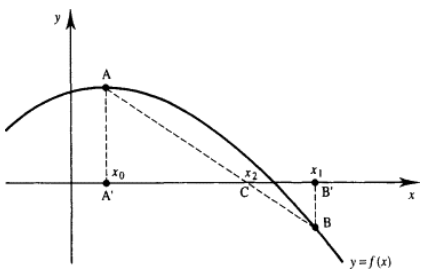
\includegraphics[width=0.5\linewidth]{img05/w05-secant} \end{center}

In general, the recursive relationship between approximated roots of the \textbf{secant method} is given by
\[
x_{n+1} = x_n -\frac{x_n-x_{n-1}}{f(x_n)-f(x_{n-1})} f(x_n), \text{ for } n =0, 1, \cdots 
\]
\url{https://github.com/pengdsci/MAT325/raw/main/w05/img/w05-betterSecantAnimation.gif}

\hypertarget{secant-algorithm-and-implementation}{%
\section{Secant Algorithm and Implementation}\label{secant-algorithm-and-implementation}}

We develop the following pseudo-code of the secant method.

\begin{verbatim}
INPUT:  f(x)            (satisfying f(x) = 0)
        x0              (initial value 1)
        x1              (initial value 2)

STEP 1: x0
        x1              (f(x0)*f(x1) must be negative)
        M = 200
        TOL = 10^(-6)
        n = 0
        ERR = |x1 - x0|  
STEP 2: WHILE ERR > TOL DO
           n = n + 1
           new.x = x1 - ((x1-x0)/(f(x1)-f(x0)))*f(x1)
           ERR = |new.x - x1|
           IF ERR < TOL DO:
              OUTPUT        (results and optional relevant info)
              STOP
           ENDIF
           IF ERR >= TOL DO:
              OUTPUT        (message or intermediate outputs)
              x1 = new.x    (update)
              x0 = x1
           ENDIF
           IF n == M DO:
             OUTPUT         (warning messages)
             STOP
           ENDIF
        ENDWHILE
\end{verbatim}

\hypertarget{implementation-with-r}{%
\subsection{Implementation with R}\label{implementation-with-r}}

We next write an R function to implement the secant method.

\begin{Shaded}
\begin{Highlighting}[]
\DocumentationTok{\#\#\#\#\#\#\#\#\#\#\#\#\#\#\#\#\#\#\#\#\#\#\#\#\#\#\#\#\#\#\#\#\#\#\#\#\#\#\#\#}
\DocumentationTok{\#\#     Root Finding: Secant Method}
\DocumentationTok{\#\#\#\#\#\#\#\#\#\#\#\#\#\#\#\#\#\#\#\#\#\#\#\#\#\#\#\#\#\#\#\#\#\#\#\#\#\#\#\#\#}
\NormalTok{Secant.Method }\OtherTok{=} \ControlFlowTok{function}\NormalTok{(fn,            }\CommentTok{\# input function}
\NormalTok{                  TOL,                  }\CommentTok{\# error tolerance }
\NormalTok{                  max.iter,             }\CommentTok{\# max allowed iterations}
\NormalTok{                  x1,                   }\CommentTok{\# initial value \#1}
\NormalTok{                  x2                    }\CommentTok{\# initial value \#2}
\NormalTok{                  )\{}
\NormalTok{  ctr }\OtherTok{=} \DecValTok{0}                \CommentTok{\# counter of iteration}
\NormalTok{  ERR }\OtherTok{=} \FunctionTok{abs}\NormalTok{(x2 }\SpecialCharTok{{-}}\NormalTok{ x1)     }\CommentTok{\# initial error {-} width of initial interval}
  \CommentTok{\# Define a data frame (data table) to store the output of each iteration}
\NormalTok{  ERR.table }\OtherTok{=}  \FunctionTok{data.frame}\NormalTok{(}\AttributeTok{Iteration =} \DecValTok{1}\SpecialCharTok{:}\NormalTok{max.iter,   }
                          \AttributeTok{Est.root =} \FunctionTok{rep}\NormalTok{(}\ConstantTok{NA}\NormalTok{, max.iter),}
                          \AttributeTok{Abs.error =} \FunctionTok{rep}\NormalTok{(}\ConstantTok{NA}\NormalTok{, max.iter))}
  \ControlFlowTok{while}\NormalTok{(ERR }\SpecialCharTok{\textgreater{}}\NormalTok{ TOL)\{ }
\NormalTok{      ctr }\OtherTok{=}\NormalTok{ ctr }\SpecialCharTok{+} \DecValTok{1}
\NormalTok{      new.x }\OtherTok{=}\NormalTok{ x2 }\SpecialCharTok{{-}} \FunctionTok{fn}\NormalTok{(x2) }\SpecialCharTok{*}\NormalTok{ (x2 }\SpecialCharTok{{-}}\NormalTok{ x1) }\SpecialCharTok{/}\NormalTok{ (}\FunctionTok{fn}\NormalTok{(x2) }\SpecialCharTok{{-}} \FunctionTok{fn}\NormalTok{(x1))}
\NormalTok{      ERR }\OtherTok{=} \FunctionTok{abs}\NormalTok{(new.x }\SpecialCharTok{{-}}\NormalTok{ x2)}
      \ControlFlowTok{if}\NormalTok{(ERR }\SpecialCharTok{\textless{}}\NormalTok{ TOL)\{}
\NormalTok{         ERR.table[ctr,] }\OtherTok{=} \FunctionTok{c}\NormalTok{(ctr, new.x, ERR)}
         \ControlFlowTok{break}
\NormalTok{         \} }\ControlFlowTok{else}\NormalTok{\{}
\NormalTok{            ERR.table[ctr,] }\OtherTok{=} \FunctionTok{c}\NormalTok{(ctr, new.x, ERR)}
            \CommentTok{\# updating the two values. }\AlertTok{CAUTION}\CommentTok{: order matters}
\NormalTok{            x1 }\OtherTok{=}\NormalTok{ x2}
\NormalTok{            x2 }\OtherTok{=}\NormalTok{ new.x}
\NormalTok{         \}}
        \ControlFlowTok{if}\NormalTok{(ctr }\SpecialCharTok{==}\NormalTok{ max.iter)\{}
         \CommentTok{\#cat("\textbackslash{}n\textbackslash{}nThe maximum number of iterations attained!\textbackslash{}n\textbackslash{}n\textbackslash{}n")}
         \ControlFlowTok{break}
\NormalTok{       \}}
\NormalTok{   \}                     }\CommentTok{\# close the while{-}loop}
  \ControlFlowTok{if}\NormalTok{(ctr}\SpecialCharTok{==}\NormalTok{max.iter)\{}
    \FunctionTok{pander}\NormalTok{(}\FunctionTok{data.frame}\NormalTok{(}\AttributeTok{message =} \StringTok{"The maximum number of iterations attained!"}\NormalTok{))}
\NormalTok{  \} }\ControlFlowTok{else}\NormalTok{\{}
  \FunctionTok{na.omit}\NormalTok{(ERR.table)     }\CommentTok{\# delete rows with NAs (missing values)}
\NormalTok{  \}}
\NormalTok{\}                        }\CommentTok{\# close the function environment}
\end{Highlighting}
\end{Shaded}

\hypertarget{numerical-examples}{%
\subsection{Numerical Examples}\label{numerical-examples}}

\textbf{Example 1}: Find a root of equation \(x^3+x^2+6x+18 = 0\).

\textbf{Solution}: we use the above R function of the Newton method to find the approximated root of the equation.

\begin{Shaded}
\begin{Highlighting}[]
\CommentTok{\# define the function f(x) that satisfies f(x) = 0}
\NormalTok{example01.func }\OtherTok{=} \ControlFlowTok{function}\NormalTok{(x)\{x}\SpecialCharTok{\^{}}\DecValTok{3}\SpecialCharTok{+}\NormalTok{x}\SpecialCharTok{\^{}}\DecValTok{2}\SpecialCharTok{+}\DecValTok{6}\SpecialCharTok{*}\NormalTok{x}\SpecialCharTok{+}\DecValTok{18}\NormalTok{ \}}
\DocumentationTok{\#\#\#}
\NormalTok{xx }\OtherTok{=} \FunctionTok{seq}\NormalTok{(}\SpecialCharTok{{-}}\DecValTok{5}\NormalTok{,}\DecValTok{5}\NormalTok{, }\AttributeTok{length=}\DecValTok{500}\NormalTok{)    }\CommentTok{\# 500 evenly x{-}values evenly spread on [{-}5, 5]}
\NormalTok{yy }\OtherTok{=} \FunctionTok{example01.func}\NormalTok{(xx)       }\CommentTok{\# the corresponding y values}
\FunctionTok{plot}\NormalTok{(xx, yy, }\AttributeTok{type =} \StringTok{"l"}\NormalTok{, }\AttributeTok{xlab =}\StringTok{""}\NormalTok{, }\AttributeTok{ylab=}\StringTok{""}\NormalTok{, }\AttributeTok{main=}\StringTok{""}\NormalTok{, }\AttributeTok{lwd =} \DecValTok{2}\NormalTok{, }\AttributeTok{col =} \StringTok{"blue"}\NormalTok{)}
\FunctionTok{abline}\NormalTok{(}\AttributeTok{h=}\DecValTok{0}\NormalTok{, }\AttributeTok{col =} \StringTok{"darkred"}\NormalTok{, }\AttributeTok{lty =} \DecValTok{2}\NormalTok{)}
\end{Highlighting}
\end{Shaded}

\begin{center}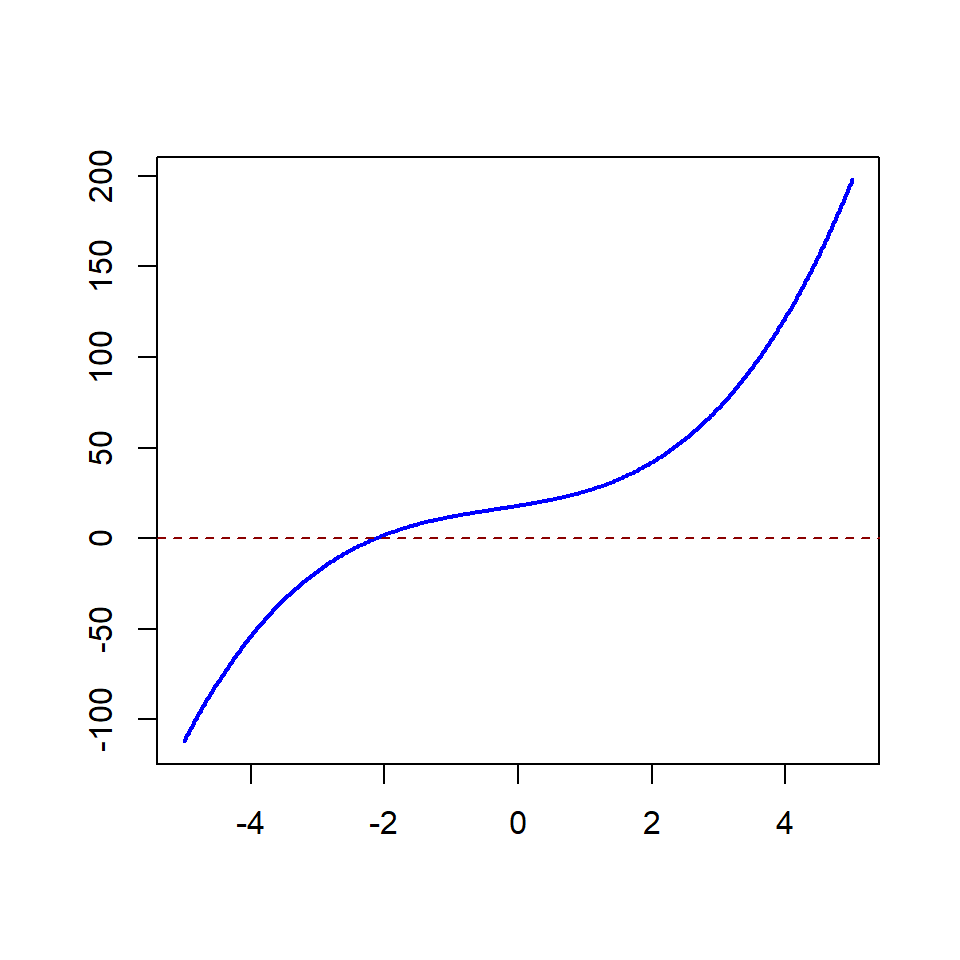
\includegraphics{MAT325EB_files/figure-latex/unnamed-chunk-77-1} \end{center}

Based on the above graph, we search a root over \([-5, 5]\) in the follwoing function call.

\begin{Shaded}
\begin{Highlighting}[]
\CommentTok{\# call the function}
\NormalTok{error.matrix }\OtherTok{=} \FunctionTok{Secant.Method}\NormalTok{(}\AttributeTok{fn =}\NormalTok{ example01.func,       }\CommentTok{\# input function}
                      \AttributeTok{TOL =} \DecValTok{10}\SpecialCharTok{\^{}}\NormalTok{(}\SpecialCharTok{{-}}\DecValTok{8}\NormalTok{),               }\CommentTok{\# error tolerance }
                      \AttributeTok{max.iter =} \DecValTok{5}\NormalTok{,               }\CommentTok{\# max allowed iterations}
                      \AttributeTok{x1 =} \SpecialCharTok{{-}}\DecValTok{5}\NormalTok{,                     }\CommentTok{\# initial value \#1}
                      \AttributeTok{x2 =} \DecValTok{5}\NormalTok{)                      }\CommentTok{\# initial value \#2}
\FunctionTok{pander}\NormalTok{(error.matrix)}
\end{Highlighting}
\end{Shaded}

\begin{verbatim}
## Warning in pander.default(error.matrix): No pander.method for "knit_asis", reverting to default.
\end{verbatim}

\begin{itemize}
\item
  \begin{longtable}[]{@{}
    >{\centering\arraybackslash}p{(\columnwidth - 0\tabcolsep) * \real{0.3333}}@{}}
  \toprule\noalign{}
  \begin{minipage}[b]{\linewidth}\centering
  message
  \end{minipage} \\
  \midrule\noalign{}
  \endhead
  \bottomrule\noalign{}
  \endlastfoot
  The maximum number of
  iterations attained! \\
  \end{longtable}
\end{itemize}

The error plot is given by

\begin{Shaded}
\begin{Highlighting}[]
\ControlFlowTok{if}\NormalTok{(}\FunctionTok{length}\NormalTok{(}\FunctionTok{dim}\NormalTok{(error.matrix))}\SpecialCharTok{\textgreater{}}\DecValTok{0}\NormalTok{)\{ }
  \DocumentationTok{\#\#\#}
\NormalTok{  Error }\OtherTok{=}\NormalTok{ error.matrix}\SpecialCharTok{$}\NormalTok{Abs.error}
\NormalTok{  nitr }\OtherTok{=} \FunctionTok{length}\NormalTok{(Error)}
  \FunctionTok{plot}\NormalTok{(}\DecValTok{1}\SpecialCharTok{:}\NormalTok{nitr, Error, }\AttributeTok{type =} \StringTok{"l"}\NormalTok{, }\AttributeTok{lwd =} \DecValTok{2}\NormalTok{, }\AttributeTok{col =} \StringTok{"blue"}\NormalTok{,}
             \AttributeTok{main=}\StringTok{"Error Plot"}\NormalTok{,}
             \AttributeTok{xlim =} \FunctionTok{c}\NormalTok{(}\DecValTok{0}\NormalTok{,nitr}\SpecialCharTok{+}\DecValTok{1}\NormalTok{),}
             \AttributeTok{ylim =} \FunctionTok{c}\NormalTok{(}\DecValTok{0}\NormalTok{, }\FunctionTok{max}\NormalTok{(Error)),}
             \AttributeTok{xlab =} \StringTok{"Iteration Numbers"}\NormalTok{,}
             \AttributeTok{ylab =} \StringTok{"Absolute Error"}\NormalTok{,}
             \AttributeTok{cex.main =} \FloatTok{0.8}\NormalTok{,}
             \AttributeTok{col.main =} \StringTok{"darkred"}
\NormalTok{        )}
\NormalTok{  \}}\ControlFlowTok{else}\NormalTok{\{}
  \FunctionTok{pander}\NormalTok{(}\FunctionTok{data.frame}\NormalTok{(}\AttributeTok{meesage =}\StringTok{"The approximation error is unavailable!"}\NormalTok{))}
\NormalTok{\}}
\end{Highlighting}
\end{Shaded}

\begin{longtable}[]{@{}
  >{\centering\arraybackslash}p{(\columnwidth - 0\tabcolsep) * \real{0.4028}}@{}}
\toprule\noalign{}
\begin{minipage}[b]{\linewidth}\centering
meesage
\end{minipage} \\
\midrule\noalign{}
\endhead
\bottomrule\noalign{}
\endlastfoot
The approximation error is
unavailable! \\
\end{longtable}

\textbf{Practice Exercise}: find the solution to \(0.8(x+0.5)^3-1=0\) 0n \([0.25, 2.75]\).

\hypertarget{error-analysis-4}{%
\section{Error Analysis}\label{error-analysis-4}}

Let \(e_n = x_n - p\), then \(e_n - e_{n-1} = x_n - x_{n-1}\). From the definition of the secant method we have
\[
e_{n+1} = e_n + x_{n+1} - x_n = e_n -\frac{x_n-x_{n-1}}{f(x_n)-f(x_{n-1})}f(x_n).
\]
With some algebraic manipulation, we can express \(e_{n+1}\) as
\[
e_{n+1} = \frac{x_n-x_{n-1}}{f(x_n)-f(x_{n-1})}\frac{f(x_n)/e_n - f(x_{n-1})/e_{n-1}}{x_n-x_{n-1}}e_ne_{n-1}.
\]
Note that
\[
\frac{x_n-x_{n-1}}{f(x_n)-f(x_{n-1})} \approx \frac{1}{f^\prime(p)}
\]
After expanding \(f(x_n)\) and \(f(x_{n-1})\) at \(p\), we have
\[
\frac{f(x_n)/e_n - f(x_{n-1})/e_{n-1}}{x_n-x_{n-1}} \approx \frac{f^{\prime\prime}(p)}{2}
\]

Therefore,
\[
e_{n+1} \approx \frac{f^{\prime\prime}(p)}{2f^\prime(p)}e_ne_{n-1}
\]

Consequently,
\[
\lim_{n\to \infty}\frac{e_{n+1}}{e_ne_{n-1}} = \frac{f^{\prime\prime}(p)}{2f^\prime(p)} = C_0
\]
To find the order of convergence, we assume that \(e_{n+1} = C_ne_n^\alpha\) where \(\lim_{n \to \infty} C_n = C\). Then

\[
\lim_{n\to \infty}\frac{e_{n+1}}{e_ne_{n-1}}=\lim_{n\to \infty}\frac{C[Ce_{n-1}^\alpha]^\alpha}{Ce^\alpha_{n-1}e_{n-1}} = \lim_{n\to\infty}C^\alpha e_{n-1}^{\alpha^2-\alpha -1} = C_0.
\]

This implies that
\[
\alpha^2 -\alpha - 1 = 0
\]
The positive root of the above equation is
\[
\alpha = \frac{1+\sqrt{5}}{2} \approx 1.62
\]

Therefore, the convergence order for the secant method is between linear and quadratic orders -- we call this \textbf{super-linear} convergence!

\hfill\break

\hypertarget{false-position-method}{%
\section{False Position Method}\label{false-position-method}}

The method of False Position (also called Regula Falsi) generates approximations using the x-coordinates of successive secant lines defined prior approximated roots in such a ways that the actual roots is always \([x_n, x_{n-1}]\) in the n-th iteration. \textbf{\color{red}Programmatically, it is the secant method with an additional control statement.}

\begin{quote}
First choose initial approximations \(p_0\) and \(p_1\) with \(f ( p_0) \times f ( p_1) < 0\). The approximation \(p_2\) is chosen in the same manner as in the Secant method, as the x-intercept of the line joining \(( p_0, f ( p_0))\) and \(( p_1, f ( p_1))\). To decide which secant line to use to compute \(p_3\), consider \(f ( p_2) \times f ( p_1)\), or more correctly \(\text{sgn} f ( p_2) \times \text{sgn} f ( p_1)\)
\end{quote}

\begin{quote}
\begin{itemize}
\tightlist
\item
  If \(\text{sgn} f ( p_2) \times \text{sgn} f ( p_1) < 0\), then \(p_1\) and \(p_2\) bracket a root. Choose \(p_3\) as the x-intercept of the line joining \(( p_1, f ( p_1))\) and \(( p_2, f ( p_2))\).
\end{itemize}
\end{quote}

\begin{quote}
\begin{itemize}
\tightlist
\item
  If not, choose \(p_3\) as the x-intercept of the line joining \(( p_0, f ( p_0))\) and \(( p_2, f ( p_2))\), and then interchange the indices on \(p_0\) and \(p_1\).
\end{itemize}
\end{quote}

\hfill\break

\begin{center}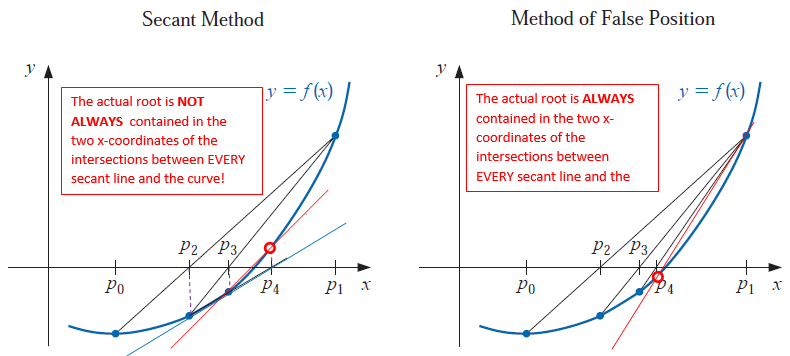
\includegraphics[width=0.8\linewidth]{img05/w05-SecantFalsePosition} \end{center}

The following is an animated graph showing the process of search the root using false position method.

\url{https://github.com/pengdsci/MAT325/raw/main/w05/img/w05-regula.gif}

Finally, the order of convergence of \textbf{false position method} is same as the \textbf{secant method}.

\hypertarget{lagrange-interpolation}{%
\chapter{Lagrange Interpolation}\label{lagrange-interpolation}}

In many computational applications, one must approximate an intractable real-valued function \(f(x)\) with a computationally tractable function \(\hat{f}(x)\). Broadly speaking, there are two types of function approximation problems that arise often in real-world applications: interpolation and functional equation problems.

Starting from this note, we will focus on numerical approximation problems via interpolation. We have noticed that a given continuous function can be approximated by a polynomial function. The following figure shows that \(y = e^x\) can be approximated by Taylor polynomials reasonably well.

\begin{center}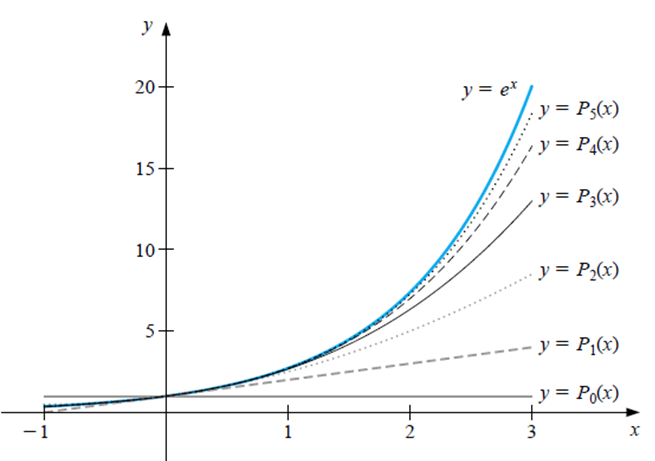
\includegraphics[width=0.5\linewidth]{img05/w05-TaylorApprox2NaturalBaseExp} \end{center}

where

\[
P_n(x) = 1 + x + \frac{x^2}{2!} + \frac{x^3}{3!} + \cdots + \frac{x^n}{n!}.
\]

Note that the Taylor expansion of \(y = e^x\) is given by

\[
y = e^x = P_n(x) + R_n(x)
\]

With

\[
R_n(x) = \frac{e^{\xi}x^{n+1}}{(n+1)!} \ \ \text{ for some } \xi \in (0, x).
\]

It is not surprising that, as \(n\) gets bigger, \(P_n(x)\) gets closer to \(y = e^x\). The next figure gives the curve of a function that is \emph{more complex} than \(e^x\). We can see a similar pattern as seen in the above figure.

\begin{center}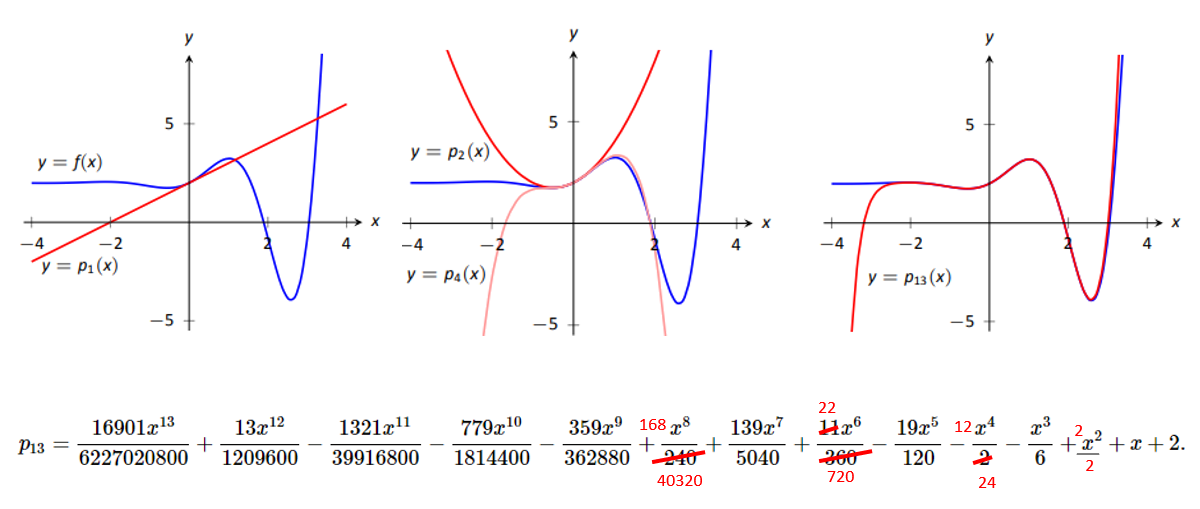
\includegraphics[width=0.9\linewidth]{img05/w05-TaylorApprox2GenFun} \end{center}

The approximation error is summarized in the following Theorem (will not prove it in this class)

\textbf{Theorem}. Let \(f(x)\) be a real-valued function that has continuous derives up to order \(n+1\), Then the remainder of the Taylor expansion at \(x = a\) (i.e., approximation error) can be expressed in the following integral form
\[
R_n^a[f(x)] = \int_a^x \frac{f^{(n+1)}(t)}{n!}(t-a)^n dt.
\]

In the above two examples, the underlying function \(f(x)\) was expanded at \(x = 0\) (i.e., Maclaurin expansion). In general, Taylor expansion (approximation) uses values of the function and its derivatives: \(f(a), f^\prime(a), f^{(2)}(a), \cdots, f^{(n)}\) and \(f^{(n+1)(\xi)}\) where \(\xi \in (a, x)\).

We can also consider Taylor expansion as a linear combination of basis functions \(\{1, x, x^2, x^3, \cdots, x^n, \cdots \}\).

There are several obvious disadvantages of the Taylor polynomial approximation:

\begin{itemize}
\item
  \(y = f(x)\) must be explicitly given and is \(n\)-th order differentiable. That is, to get an n-th degree Taylor polynomial, we need to assume \(f(x)\) to have an n-th order derivative.
\item
  The approximation is very well in the neighborhood of \(x= a\) at which the function \(y = f(x)\) is expanded (via Taylor expansion) but is poor far away from the neighborhood.
\end{itemize}

\textbf{\color{red}A natural question}: \emph{whether we can sample a set of points on the curve of \(y = f(x)\) and then find a lower degree (than Taylor) polynomial for approximating \(y = f(x)\) such that \(P_n(x_i) = f(x_i)\)}.

The answer to the question is \textbf{YES}. Several methods using this idea will be introduced in the next few notes.

\hypertarget{concepts-of-interpolation-method}{%
\section{Concepts of Interpolation Method}\label{concepts-of-interpolation-method}}

A function is said to \textbf{interpolate} a set of data points if it passes through those points.

\textbf{Definition}: The function \(y = f(x)\) interpolates the data points \(\{(x_1, y_1), (x_2, y_2), \cdots, (x_n, x_n)\}\) if \(y_i = P_n(x_i)\) for each \(1 \le i \le n\).

Since \(f(x)\) is a function; \(x_i\)'s must be all distinct in order for a function to pass through them.

\hfill\break

\hypertarget{data-fitting-interpolation}{%
\subsection{Data-fitting / Interpolation:}\label{data-fitting-interpolation}}

For the following given points samples from an \textbf{unknown function} \(f(x)\):

\begin{longtable}[]{@{}llllll@{}}
\toprule\noalign{}
\(x\) & \(x_0\) & \(x_1\) & \(x_2\) & \(\cdots\) & \(x_n\) \\
\midrule\noalign{}
\endhead
\bottomrule\noalign{}
\endlastfoot
\(y\) & \(y_0\) & \(y_1\) & \(y_2\) & \(\cdots\) & \(y_n\) \\
\end{longtable}

and we try to find a polynomial \(P_n(x)\) of degree \(\le n\) for which,

\[
P_n(x_i) = y_i, \  \ \text{ for } \ \ 0 \le i \le n.
\]
such a polynomial is said to interpolate the data (data fitting). This type of question is very common in almost areas that produce data.

\textbf{Existence of Polynomial Interpolation}: if \(\{x_0, x_1, x_2, \cdots, x_n \}\) are distinct real numbers, then for arbitrary values \(\{y_0, y_1, y_2, \cdots, y_n \}\) there is a unique polynomial \(P_n(x)\) of degree \(\le n\) such that

\[
P_n(x_i) = y_i, \ \ \text{ for } 0 \le i \le n.
\]

\textbf{Proof}. For any polynomial \(P_n(x)\) of degree \(\le n\), we have the following form :

\[
P_n(x) = a_0 + a_1x + a_2 x^2 + \cdots + a_n x^n.
\]

To determine the polynomial \(P_n(x)\) is to find the coefficient \(a_i\)'s. We will use the interpolation condition \(P_n(x_i) = y_i, \ \ \text{ for } 0 \le i \le n\).

\begin{center}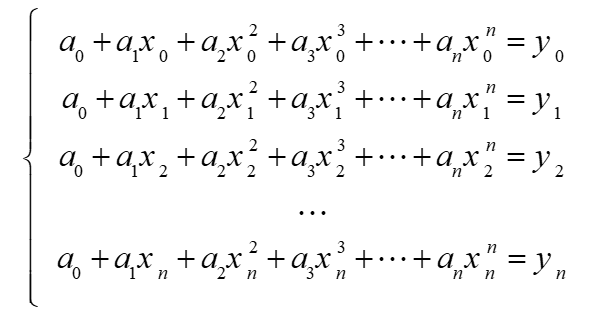
\includegraphics[width=0.5\linewidth]{img05/w05-interpolationEq} \end{center}

Note that \(\{a_0, a_1, a_2, \cdots, a_n \}\), are unknown. We rewrite it in the following matrix form

\begin{center}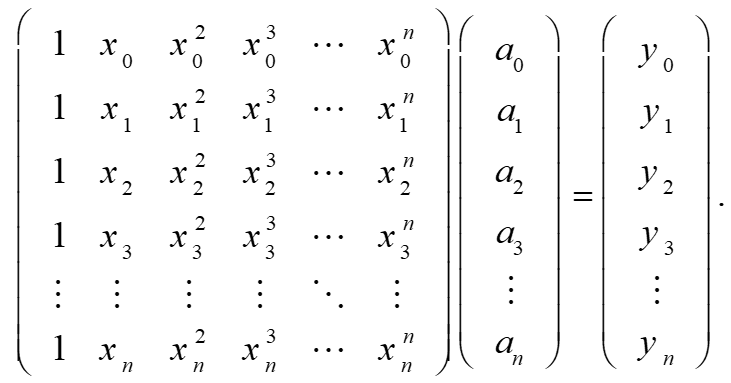
\includegraphics[width=0.6\linewidth]{img05/w05-interpolationEqMatrix} \end{center}

Since the coefficient matrix is a \textbf{Vandermonde matrix}, it is nonsingular if and only if \(\{x_0, x_1, x_2, \cdots, x_n \}\) are distinct. This imply that the system exists a unique solution \((a_0, a_1, a_2, \cdots, a_n)^T\) if and only if \(\{x_0, x_1, x_2, \cdots, x_n \}\) are distinct since the determinant of that matrix is

\[
\prod_{1 \le i < j \le n}(x_i-x_j)
\]

Hence, there exists a unique polynomial \(P_n(x)\) of degree \(\le n\) if \(\{x_0, x_1, x_2, \cdots, x_n \}\) are distinct.

\hfill\break

\hypertarget{functional-equation-curve-approximation}{%
\subsection{Functional Equation (Curve Approximation)}\label{functional-equation-curve-approximation}}

Another type of interpolation problem is formulated as follows: given a set of \(\{ x_0, x_1, x_3, \cdots, x_n\}\) and a continuous function \(f(x)\), find a polynomial \(P_n(x)\) of degree less than or equal to n such that \(P_n(x_i) = f(x_i)\) for \(0 \le i \le n\).

The Newton interpolation is one type of this problems. We will introduce this method in a subsequent note.

\hfill\break

\hypertarget{the-lagrange-interpolation}{%
\section{The Lagrange Interpolation}\label{the-lagrange-interpolation}}

The basic idea of Lagrange interpolation is approximate a function by using a linear combination of Lagrange basis polynomials defined based on a given set of distinct points \(\{(x_0, y_0), (x_1, y_1), (x_2, y_2), \cdots, (x_n, y_n)\}\) sampled from a curve of a function \(f(x)\) with an unknown analytic expression. The given points are called interpolation nodes.

Next, we use several special interpolations to illustrate the construction of Lagrange basis polynomials.

\hypertarget{linear-lagrange-interpolation}{%
\subsection{Linear Lagrange Interpolation}\label{linear-lagrange-interpolation}}

Assume that we are given two distinct points \(\{(x_0, y_0), (x_1, y_1)\}\). The objective is to find an interpolation ``\emph{polynomial}'' that passes through the two points. Intuitively, we use the following two-point form

\[
y = \frac{y_1 - y_0}{x_1 - x_0}(x - x_0) + y_0
\]
The above function is linear (degree 1 polynomial). We use

\[
p_1(x) = \frac{y_1 - y_0}{x - x_0}(x - x_0) + y_0.
\]
Next, we re-express the above degree one polynomial in the following

\[
p_1(x) = y_1\frac{x-x_0}{x_1-x_0} + y_0\left(1-\frac{x-x_0}{x_1-x_0} \right) = y_1\frac{x-x_0}{x_1-x_0} + y_0\frac{x-x_1}{x_0-x_1}
\]

We denote

\[
L_0(x) = \frac{x-x_1}{x_0-x_1} \ \ \text{ and } \ \ L_1(x) = \frac{x-x_0}{x_1-x_0} .
\]

\(L_0(x)\) and \(L_1(x)\) are both degree-one polynomials. They are called \textbf{Lagrange Basis Polynomials with degree 1}.

\textbf{Observations of Lagrange Basis Polynomials}: For \(i, j = 0, 1\),

\[
L_i(x_j) = \begin{cases} 
      1 & i = j \\
      0 & i \ne j. 
   \end{cases}
\]

The degree-one interpolation polynomial is expressed as \(p_1(x) = y_0 L_0(x) + y_1 L_1(x)\). The following figure illustrates how the interpolated polynomial is expressed as the linear combination of the \textbf{Lagrange Basis Polynomials}.

\begin{center}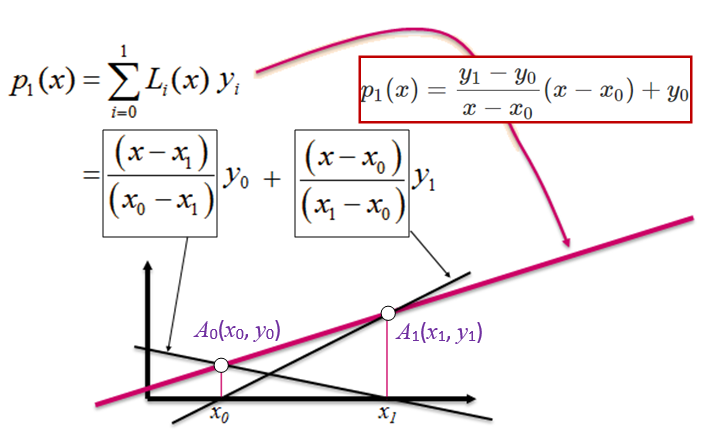
\includegraphics[width=0.5\linewidth]{img05/w05-degreeOneLagrangeInterpolation} \end{center}

We can check that \(p_1(x_0) = y_0\) and \(p_1(x_1) = y_1.\).

\hfill\break

\hypertarget{quadratic-lagrange-interpolation}{%
\subsection{Quadratic Lagrange Interpolation}\label{quadratic-lagrange-interpolation}}

Quadratic Lagrange interpolation assumes that three distinct points were sampled from the curve.

\begin{longtable}[]{@{}llll@{}}
\toprule\noalign{}
\(x\) & \(x_0\) & \(x_1\) & \(x_2\) \\
\midrule\noalign{}
\endhead
\bottomrule\noalign{}
\endlastfoot
\(y\) & \(y_0\) & \(y_1\) & \(y_2\) \\
\end{longtable}

The objective is to find a polynomial \(p_2(x)\) of degree \(\le 2\) such that

\[
p_2(x_i) = y_i, \ \ \text{ for } i = 1, 2, 3.
\]

we construct the basis \(L_0(x), L_1(x), L_2(x)\) such that

\[
L_i(x_j) = \begin{cases} 
      1 & i = j \\
      0 & i \ne j. 
   \end{cases}
\]

We only construct the basis function \(L_0(x)\) associated with the point \(x_0\). Since \(x_1\) and \(x_2\) are zeros of \(L_0(x)\), it should have the following form

\[
L_0(x) = c(x-x_1)(x-x_2).
\]
Since \(L_0(x_0) = 1\), which implies that

\[
c = \frac{1}{(x_0-x_1)(x_0-x_2)}
\]

Therefore,

\[
L_0 = \frac{(x-x_1)(x-x_2)}{(x_0-x_1)(x_0-x_2)}
\]

Similarly, we can construct \(L_1(x)\) and \(L_2(x)\) in the following

\[
L_1(x) = \frac{(x-x_0)(x-x_2)}{(x_1-x_0)(x_1-x_2)} \ \ \text{ and } \ \ L_2(x) = \frac{(x-x_0)(x-x_1)}{(x_2-x_0)(x_2-x_1)}
\]
Hence the interpolation polynomial is as follows

\[
p_2(x) = y_0L_0(x) + y_1 L_1(x) + y_2 L_2(x)
\]

\begin{center}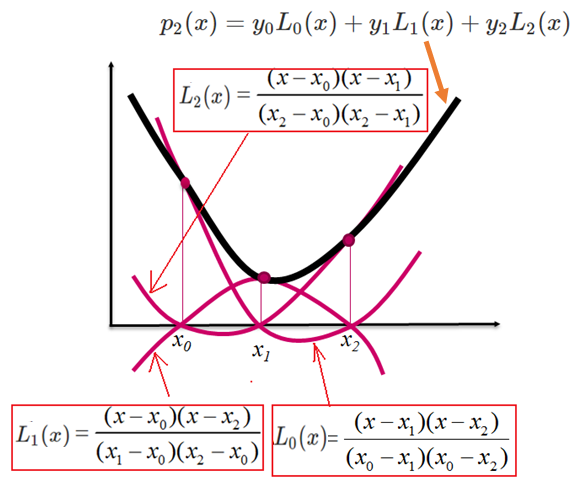
\includegraphics[width=0.55\linewidth]{img05/w05-degreeTwoLagrangeInterpolation} \end{center}

\hfill\break

\hypertarget{general-lagrange-interpolation}{%
\subsection{General Lagrange Interpolation}\label{general-lagrange-interpolation}}

Assume now that we are given the following distinct points

\begin{longtable}[]{@{}llllll@{}}
\toprule\noalign{}
\(x\) & \(x_0\) & \(x_1\) & \(x_2\) & \(\cdots\) & \(x_n\) \\
\midrule\noalign{}
\endhead
\bottomrule\noalign{}
\endlastfoot
\(y\) & \(y_0\) & \(y_1\) & \(y_2\) & \(\cdots\) & \(y_n\) \\
\end{longtable}

then a unique polynomial \(p_n(x)\) of degree at most \(n\) exists with

\[
p_n(x) = y_k
\]
This polynomial is explicitly defined as follows

\[
p_n(x) = y_0L_{n,0}(x) + y_1 L_{n,1}(x) + \cdots + y_nL_{n,n}(x),
\]

where

\[
L_{n,k} = \frac{(x-x_0)(x-x_1)\cdots(x-x_{k-1})(x-x_{k+1})\cdots(x_k-x_n)}{(x_k-x_0)(x_k-x_1)\cdots(x_k-x_{k-1})(x_k-x_{k+1})\cdots(x_k-x_n)}.
\]

\hypertarget{lagrange-algorithm-and-implementation}{%
\section{Lagrange Algorithm and Implementation}\label{lagrange-algorithm-and-implementation}}

The algorithm of the Lagrange interpolation involves two nested iterative processes:

\begin{itemize}
\item
  Approximated individual basis polynomial and evaluate it at a given x-value (including the x-coordinates in the approximating notes);
\item
  Estimated the set of estimated polynomials with the approximated value of Pn(x).
\end{itemize}

\hypertarget{pseudo-code}{%
\subsection{Pseudo-code}\label{pseudo-code}}

The pseudo-code is given by:

\begin{verbatim}
INPUT: x1, x2, ... ,xn
       y1, y2, ... ,yn
        (or f(x1), f(x2), ..., f(xn))
       pred.x  

OUTPUT: return Pn(x)

STEP 1: set initial values
        Pn = 0     (initial value of interpolated polynomial)
        LP = 1     (vector with all 1s)

Step 2: FOR i = 1, 2, ..., n. DO
        STEP 3: FOR j = 1, 2, ..., n. DO
                    IF i != j DO:
                       LP = LP*(pred.x-xj)/(xi-xj)
                    ENDIF
                ENDFOR
        STEP 4  Pn = LP*yi + Pn
        ENDFOR        
STEP 5: OUTPUT Pn              
\end{verbatim}

\hypertarget{r-function-with-scalar-input}{%
\subsection{R Function with Scalar Input}\label{r-function-with-scalar-input}}

The next function takes only a single x value and returns the value of the approximated polynomial at the provided x value.

\begin{Shaded}
\begin{Highlighting}[]
\DocumentationTok{\#\#\#\#\#\#\#\#\#\#\#\#\#\#\#\#\#\#\#\#\#\#\#\#\#\#\#\#\#\#\#\#\#\#\#\#\#\#\#\#\#\#\#\#\#\#\#\#\#\#\#\#\#\#\#}
\DocumentationTok{\#\#        Lagrange Interpolation}
\DocumentationTok{\#\#\#\#\#\#\#\#\#\#\#\#\#\#\#\#\#\#\#\#\#\#\#\#\#\#\#\#\#\#\#\#\#\#\#\#\#\#\#\#\#\#\#\#\#\#\#\#\#\#\#\#\#\#\#}
\NormalTok{LagrangeInterpolation }\OtherTok{=}\ControlFlowTok{function}\NormalTok{(}
\NormalTok{                        pred.x,      }\CommentTok{\# scalar x for eval Pn() }
                        \AttributeTok{fn =} \ConstantTok{NULL}\NormalTok{,   }\CommentTok{\# input function or}
                        \AttributeTok{yvec =} \ConstantTok{NULL}\NormalTok{, }\CommentTok{\# input y{-}coordinates}
\NormalTok{                        xvec         }\CommentTok{\# input x{-}coordinates}
\NormalTok{                        )\{}
     \CommentTok{\# }
     \ControlFlowTok{if}\NormalTok{(}\FunctionTok{length}\NormalTok{(yvec) }\SpecialCharTok{==} \DecValTok{0}\NormalTok{) yvec }\OtherTok{=} \FunctionTok{fn}\NormalTok{(xvec) }\CommentTok{\#}
\NormalTok{     n }\OtherTok{=} \FunctionTok{length}\NormalTok{(xvec)       }\CommentTok{\# input x{-}coordinates}
\NormalTok{     Pn }\OtherTok{=} \DecValTok{0}
     \ControlFlowTok{for}\NormalTok{ (i }\ControlFlowTok{in} \DecValTok{1}\SpecialCharTok{:}\NormalTok{n)\{}
\NormalTok{         LP }\OtherTok{=} \DecValTok{1}
         \ControlFlowTok{for}\NormalTok{ (j }\ControlFlowTok{in}\NormalTok{ (}\DecValTok{1}\SpecialCharTok{:}\NormalTok{n)[}\SpecialCharTok{{-}}\NormalTok{i])\{  }
\NormalTok{              LP }\OtherTok{=}\NormalTok{ LP }\SpecialCharTok{*}\NormalTok{ (pred.x }\SpecialCharTok{{-}}\NormalTok{ xvec[j])}\SpecialCharTok{/}\NormalTok{(xvec[i] }\SpecialCharTok{{-}}\NormalTok{ xvec[j])}
\NormalTok{             \}}
\NormalTok{         Pn }\OtherTok{=}\NormalTok{ Pn }\SpecialCharTok{+}\NormalTok{ LP }\SpecialCharTok{*}\NormalTok{ yvec[i]}
\NormalTok{       \}}
\NormalTok{   Pn}
\NormalTok{  \}}
\end{Highlighting}
\end{Shaded}

\hfill\break

\textbf{Example 1}: Find a Lagrange polynomial to approximate the function \(f(x) = e^x\cos(3x)\) and estimate the value of \(f(x)\) at \(x = 0.5\) and \(0.3\) respectively.

\textbf{Solution}: We use the above R function to estimate \(f(x)\) at \(x = 0.5\) and \(0.3\). We also print out the true values \(f(x)\) at \(x = 0.5\) and \(0.3\) for comparison.

\begin{Shaded}
\begin{Highlighting}[]
\NormalTok{fn}\OtherTok{=}\ControlFlowTok{function}\NormalTok{(x) }\FunctionTok{exp}\NormalTok{(x)}\SpecialCharTok{*}\FunctionTok{cos}\NormalTok{(}\DecValTok{3}\SpecialCharTok{*}\NormalTok{x)}
\NormalTok{approx.val0}\FloatTok{.3} \OtherTok{=} \FunctionTok{LagrangeInterpolation}\NormalTok{(}\AttributeTok{fn=}\NormalTok{fn, }\AttributeTok{xvec=}\FunctionTok{c}\NormalTok{(}\DecValTok{0}\NormalTok{, }\FloatTok{0.3}\NormalTok{, }\FloatTok{0.6}\NormalTok{), }\AttributeTok{pred.x =} \FloatTok{0.3}\NormalTok{)}
\NormalTok{approx.val0}\FloatTok{.5} \OtherTok{=} \FunctionTok{LagrangeInterpolation}\NormalTok{(}\AttributeTok{fn=}\NormalTok{fn, }\AttributeTok{xvec=}\FunctionTok{c}\NormalTok{(}\DecValTok{0}\NormalTok{, }\FloatTok{0.3}\NormalTok{, }\FloatTok{0.6}\NormalTok{), }\AttributeTok{pred.x =} \FloatTok{0.5}\NormalTok{)}
\NormalTok{true.val }\OtherTok{=} \FunctionTok{fn}\NormalTok{(}\FunctionTok{c}\NormalTok{(}\FloatTok{0.3}\NormalTok{,}\FloatTok{0.5}\NormalTok{))}
\FunctionTok{pander}\NormalTok{(}\FunctionTok{cbind}\NormalTok{(}\AttributeTok{approx.val0.3 =}\NormalTok{ approx.val0}\FloatTok{.3}\NormalTok{, }\AttributeTok{true.val0.3 =}\NormalTok{ true.val[}\DecValTok{1}\NormalTok{],  }
             \AttributeTok{approx.val0.5 =}\NormalTok{ approx.val0}\FloatTok{.5}\NormalTok{, }\AttributeTok{true.val0.5 =}\NormalTok{ true.val[}\DecValTok{2}\NormalTok{]))}
\end{Highlighting}
\end{Shaded}

\begin{longtable}[]{@{}
  >{\centering\arraybackslash}p{(\columnwidth - 6\tabcolsep) * \real{0.2222}}
  >{\centering\arraybackslash}p{(\columnwidth - 6\tabcolsep) * \real{0.1944}}
  >{\centering\arraybackslash}p{(\columnwidth - 6\tabcolsep) * \real{0.2222}}
  >{\centering\arraybackslash}p{(\columnwidth - 6\tabcolsep) * \real{0.2222}}@{}}
\toprule\noalign{}
\begin{minipage}[b]{\linewidth}\centering
approx.val0.3
\end{minipage} & \begin{minipage}[b]{\linewidth}\centering
true.val0.3
\end{minipage} & \begin{minipage}[b]{\linewidth}\centering
approx.val0.5
\end{minipage} & \begin{minipage}[b]{\linewidth}\centering
true.val0.5
\end{minipage} \\
\midrule\noalign{}
\endhead
\bottomrule\noalign{}
\endlastfoot
0.8391 & 0.8391 & 0.1251 & 0.1166 \\
\end{longtable}

\hypertarget{r-function-with-vector-input}{%
\subsection{R Function with Vector Input}\label{r-function-with-vector-input}}

\begin{Shaded}
\begin{Highlighting}[]
\DocumentationTok{\#\#\#\#\#\#\#\#\#\#\#\#\#\#\#\#\#\#\#\#\#\#\#\#\#\#\#\#\#\#\#\#\#\#\#\#\#\#\#\#\#\#\#\#\#\#\#\#\#\#\#\#\#\#\#}
\DocumentationTok{\#\#        Lagrange Interpolation}
\DocumentationTok{\#\#\#\#\#\#\#\#\#\#\#\#\#\#\#\#\#\#\#\#\#\#\#\#\#\#\#\#\#\#\#\#\#\#\#\#\#\#\#\#\#\#\#\#\#\#\#\#\#\#\#\#\#\#\#}
\NormalTok{Lagrange.Interpolation.Vector }\OtherTok{=}\ControlFlowTok{function}\NormalTok{(}
\NormalTok{                        pred.x,      }\CommentTok{\# vector x for eval Pn() }
                        \AttributeTok{fn =} \ConstantTok{NULL}\NormalTok{,   }\CommentTok{\# input function or}
                        \AttributeTok{yvec =} \ConstantTok{NULL}\NormalTok{, }\CommentTok{\# input y{-}coordinates}
\NormalTok{                        xvec         }\CommentTok{\# input x{-}coordinates}
\NormalTok{                        )\{}
  \CommentTok{\# }
  \ControlFlowTok{if}\NormalTok{(}\FunctionTok{length}\NormalTok{(yvec) }\SpecialCharTok{==} \DecValTok{0}\NormalTok{) yvec }\OtherTok{=} \FunctionTok{fn}\NormalTok{(xvec) }\CommentTok{\#}
\NormalTok{  n }\OtherTok{=} \FunctionTok{length}\NormalTok{(xvec)       }\CommentTok{\# input x{-}coordinates}
\NormalTok{  m }\OtherTok{=} \FunctionTok{length}\NormalTok{(pred.x)     }\CommentTok{\# number of input x values}
\NormalTok{  PV }\OtherTok{=} \FunctionTok{rep}\NormalTok{(}\DecValTok{0}\NormalTok{, m)}
  \ControlFlowTok{for}\NormalTok{ (k }\ControlFlowTok{in} \DecValTok{1}\SpecialCharTok{:}\NormalTok{m)\{}
\NormalTok{     Pn }\OtherTok{=} \DecValTok{0}
     \ControlFlowTok{for}\NormalTok{ (i }\ControlFlowTok{in} \DecValTok{1}\SpecialCharTok{:}\NormalTok{n)\{}
\NormalTok{         LP }\OtherTok{=} \DecValTok{1}
         \ControlFlowTok{for}\NormalTok{ (j }\ControlFlowTok{in}\NormalTok{ (}\DecValTok{1}\SpecialCharTok{:}\NormalTok{n)[}\SpecialCharTok{{-}}\NormalTok{i])\{  }
\NormalTok{              LP }\OtherTok{=}\NormalTok{ LP }\SpecialCharTok{*}\NormalTok{ (pred.x[k] }\SpecialCharTok{{-}}\NormalTok{ xvec[j])}\SpecialCharTok{/}\NormalTok{(xvec[i] }\SpecialCharTok{{-}}\NormalTok{ xvec[j])}
\NormalTok{             \}}
\NormalTok{         Pn }\OtherTok{=}\NormalTok{ Pn }\SpecialCharTok{+}\NormalTok{ LP }\SpecialCharTok{*}\NormalTok{ yvec[i]}
\NormalTok{       \}}
\NormalTok{     PV[k] }\OtherTok{=}\NormalTok{ Pn}
\NormalTok{    \}}
\NormalTok{   PV}
\NormalTok{  \}}
\end{Highlighting}
\end{Shaded}

\begin{Shaded}
\begin{Highlighting}[]
\NormalTok{fn}\OtherTok{=}\ControlFlowTok{function}\NormalTok{(x) }\FunctionTok{exp}\NormalTok{(x)}\SpecialCharTok{*}\FunctionTok{cos}\NormalTok{(}\DecValTok{3}\SpecialCharTok{*}\NormalTok{x)}
\NormalTok{approx.value }\OtherTok{=} \FunctionTok{Lagrange.Interpolation.Vector}\NormalTok{(}\AttributeTok{fn=}\NormalTok{fn, }\AttributeTok{xvec=}\FunctionTok{c}\NormalTok{(}\DecValTok{0}\NormalTok{, }\FloatTok{0.3}\NormalTok{, }\FloatTok{0.6}\NormalTok{), }
                                             \AttributeTok{pred.x =} \FunctionTok{c}\NormalTok{(}\FloatTok{0.3}\NormalTok{, }\FloatTok{0.5}\NormalTok{))}
\NormalTok{true.value }\OtherTok{=} \FunctionTok{fn}\NormalTok{(}\FunctionTok{c}\NormalTok{(}\FloatTok{0.3}\NormalTok{, }\FloatTok{0.5}\NormalTok{))}
\FunctionTok{pander}\NormalTok{(}\FunctionTok{rbind}\NormalTok{(}\AttributeTok{true.value=}\NormalTok{true.value, }\AttributeTok{approx.value =}\NormalTok{ approx.value))}
\end{Highlighting}
\end{Shaded}

\begin{longtable}[]{@{}
  >{\centering\arraybackslash}p{(\columnwidth - 4\tabcolsep) * \real{0.2639}}
  >{\centering\arraybackslash}p{(\columnwidth - 4\tabcolsep) * \real{0.1250}}
  >{\centering\arraybackslash}p{(\columnwidth - 4\tabcolsep) * \real{0.1250}}@{}}
\toprule\noalign{}
\endhead
\bottomrule\noalign{}
\endlastfoot
\textbf{true.value} & 0.8391 & 0.1166 \\
\textbf{approx.value} & 0.8391 & 0.1251 \\
\end{longtable}

\textbf{Example 3}: Consider Lagrange interpolation approximation of \(f(x) = \frac{1}{1+25x^2}\). The x-nodes used in the approximation are (-1.0, -0.8, -0.6, -0.4, -0.2, 0, 0.2, 0.4, 0.6, 0.8, 1). Plot the curves of \(f(x)\) and \(P_{10}(x)\).

\textbf{Solution}: Based on the given information, we use the above vector-based function to find the P\_n(x) and create a sequence of 100 x-values from {[}-1, 1{]} that are equally spaced.

\begin{Shaded}
\begin{Highlighting}[]
\NormalTok{fn}\OtherTok{=}\ControlFlowTok{function}\NormalTok{(x) }\DecValTok{1}\SpecialCharTok{/}\NormalTok{(}\DecValTok{1} \SpecialCharTok{+} \DecValTok{25}\SpecialCharTok{*}\NormalTok{x}\SpecialCharTok{\^{}}\DecValTok{2}\NormalTok{)}
\NormalTok{pred.x }\OtherTok{=} \FunctionTok{seq}\NormalTok{(}\SpecialCharTok{{-}}\DecValTok{1}\NormalTok{, }\DecValTok{1}\NormalTok{, }\AttributeTok{length =} \DecValTok{100}\NormalTok{)}
\NormalTok{xvec }\OtherTok{=} \FunctionTok{c}\NormalTok{(}\SpecialCharTok{{-}}\FloatTok{1.0}\NormalTok{, }\SpecialCharTok{{-}}\FloatTok{0.8}\NormalTok{, }\SpecialCharTok{{-}}\FloatTok{0.6}\NormalTok{, }\SpecialCharTok{{-}}\FloatTok{0.4}\NormalTok{, }\SpecialCharTok{{-}}\FloatTok{0.2}\NormalTok{, }\DecValTok{0}\NormalTok{, }\FloatTok{0.2}\NormalTok{, }\FloatTok{0.4}\NormalTok{, }\FloatTok{0.6}\NormalTok{, }\FloatTok{0.8}\NormalTok{, }\DecValTok{1}\NormalTok{)}
\DocumentationTok{\#\#}
\NormalTok{approx.value }\OtherTok{=} \FunctionTok{Lagrange.Interpolation.Vector}\NormalTok{(}\AttributeTok{fn=}\NormalTok{fn, }\AttributeTok{xvec=}\NormalTok{xvec, }
                                             \AttributeTok{pred.x =}\NormalTok{ pred.x)}
\NormalTok{true.value }\OtherTok{=} \FunctionTok{fn}\NormalTok{(pred.x)}
\FunctionTok{plot}\NormalTok{(pred.x, approx.value, }\AttributeTok{type =} \StringTok{"l"}\NormalTok{, }\AttributeTok{col =} \StringTok{"red"}\NormalTok{, }\AttributeTok{lwd =} \DecValTok{2}\NormalTok{, }\AttributeTok{lty =} \DecValTok{1}\NormalTok{,}
            \AttributeTok{main =} \StringTok{"Lagrange Interpolation"}\NormalTok{,}
             \AttributeTok{xlab =} \StringTok{""}\NormalTok{,}
             \AttributeTok{ylab =} \StringTok{""}\NormalTok{)}
\FunctionTok{lines}\NormalTok{(pred.x, true.value, }\AttributeTok{lty =} \DecValTok{2}\NormalTok{, }\AttributeTok{lwd =} \DecValTok{2}\NormalTok{, }\AttributeTok{col =} \StringTok{"blue"}\NormalTok{)}
\FunctionTok{points}\NormalTok{(xvec, }\FunctionTok{fn}\NormalTok{(xvec), }\AttributeTok{pch =} \DecValTok{19}\NormalTok{, }\AttributeTok{col =} \StringTok{"purple"}\NormalTok{, }\AttributeTok{cex =} \FloatTok{1.2}\NormalTok{)}
\FunctionTok{legend}\NormalTok{(}\StringTok{"top"}\NormalTok{, }\FunctionTok{c}\NormalTok{(}\StringTok{"Interpolated Polynomial"}\NormalTok{, }\StringTok{"Original Function"}\NormalTok{), }
       \AttributeTok{lwd=}\FunctionTok{rep}\NormalTok{(}\DecValTok{2}\NormalTok{,}\DecValTok{2}\NormalTok{), }\AttributeTok{lty=}\DecValTok{1}\SpecialCharTok{:}\DecValTok{2}\NormalTok{, }\AttributeTok{col =} \FunctionTok{c}\NormalTok{(}\StringTok{"red"}\NormalTok{, }\StringTok{"blue"}\NormalTok{), }\AttributeTok{bty=}\StringTok{"n"}\NormalTok{)}
\end{Highlighting}
\end{Shaded}

\begin{center}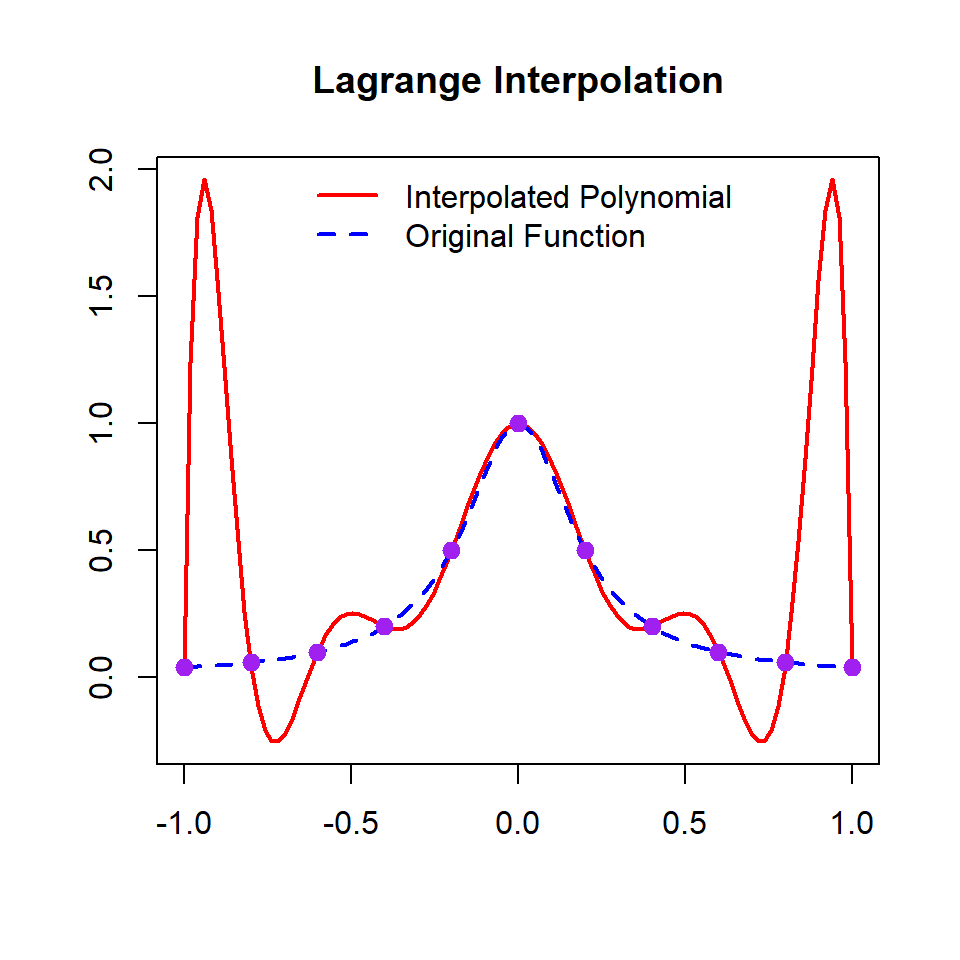
\includegraphics{MAT325EB_files/figure-latex/unnamed-chunk-92-1} \end{center}

\hypertarget{error-analysis-5}{%
\section{Error Analysis}\label{error-analysis-5}}

It is important to understand the nature of the error term when the Lagrange polynomial is used to approximate a continuous function \(f(x)\).

We can see from the expression of Lagrange basis polynomials that the error term of Lagrange interpolation should be similar to that for the Taylor polynomial, except that the factor \((x - x_0)^{n+1}\) is replaced with the product \((x - x_0)(x - x1) \cdots (x - x_n)\). This is expected because interpolation is exact at each of the \(n + 1\) nodes \(x_k\) , where we have error term \(E_n (x_k) = f(x_k) - P_n (x_k) = y_k - y_k = 0\) for \(k = 0, 1, 2, \cdots , n\).

The following theorem specifies the error term of the Lagrange interpolation.

\textbf{Theorem}:Assume that \(f \in C^{n+1}[a, b]\) and that \(x_0, x_1, \cdots , x_n \in [a, b]\) are \(n + 1\) nodes. If \(x \in [a, b]\), then

\[
f(x) = P_n(x) + E_n(x)
\]

where \(P_n(x)\) is a polynomial used to approximate \(f(x)\)

\[
f(x) \approx P_n(x) = \sum_{j=0}^n f(x_j)L_j(x) = \sum_{j=0}^n y_jL_j(x)
\]

The error term \(E_n(x)\) has the form

\[
E_n(x) = \frac{f^{(n+1)}(c)}{(n+1)!}(x-x_0)(x-x_1)\cdots(x-x_n)
\]

for some value \(c = c(x)\) that lies in the interval \([a, b]\).

\textbf{Proof} (I only prove the special case of \(n = 2\), i.e., with 3 interpolation nodes).

For given two nodes \(x_0, x_1 x_2\) and an arbitrarily chosen \(x\), If \(x = x_j (j = 0, 1, 2)\), then error \(E_2(x) = 0\).

We now assume that the arbitrarily chosen value \(x \ne x_j (j =0, 1, 2)\).

Denote \(w(t) = (t - x_0)(t - x_1)(t - x_2)\) and \(\lambda = [f(x) - P_2(x)]/w(x)\). Clearly, \(w(x) \ne 0\). We now define an auxiliary function \(\phi(t) = f(t) - P_2(t) - \lambda w(t)\). Apparently, \(\phi(x) = 0\), \(\phi(x_j) = 0\) (for \(j = 0, 1,2\)), and \(\phi \in C^3[a, b]\).

since \(f\in C^3[a,b]\) and \(\phi (t) = 0\) has four roots, \(x, x_0, x_1, x_2\) in \([a, b]\), there are 3 roots for \(\phi^\prime(t) = 0\) in the open interval \((a, b)\) according to Rolle's Theorem (special case of the Mean Value Theorem). It follows that there are 2 roots for \(\phi^{\prime\prime}(t) = 0\) in \((a, b\)) and 1 root for \(\phi^{\prime\prime\prime}(t)=0\) in \((a, b)\).

Therefore, \(\exists c = c(x)\) so that \(c(x) \in (a,b)\) and \(\phi^{\prime\prime\prime}(c) = 0\). Note that, \(\phi^{\prime\prime\prime}(t) = f^{\prime\prime\prime}(t) – P_2^{\prime\prime\prime}(t) – \lambda w^{\prime\prime\prime}(t)\).

From the definition of \(P_2(t)\) and \(w(t)\) we know that \(P_2^{\prime\prime\prime}(t) =0\) and \(w^{\prime\prime\prime}(t) = 3!\). Plugging these values into the above equation, we have \(\lambda^{\prime\prime\prime}(t)=f^{\prime\prime\prime}(t) - \lambda 3!\). Consequently, \(f^{\prime\prime\prime}(c) - \lambda 3! =0\). Recall that \(\lambda = [f(x) - P_2(x)]/w(x)\) and \(w(x) = (x - x_0)(x - x_1)(x - x_2)\). We rewrite \(f^{\prime\prime\prime}(c) - \lambda 3! =0\) as follows
\[
f^{\prime\prime\prime}(c) - \frac{3![f(x) - P2(x)]}{(x - x0)(x - x1)(x - x2)} = 0
\].

Therefore,

\[
f(x) - P_2(x) = \frac{f^{\prime\prime\prime}(c) }{3!}(x - x_0)(x - x_1)(x - x_2).
\]
The proof is completed.

The following corollary gives the error bound explicitly.

\textbf{Corollary}: Assume that \(f \in C^{n+1}[a, b]\) and \(|f^{(n+1)}(x)| \le M\) for all \(x \in [a, b]\). Assume also that nodes \(x_0, x_1, \cdots , x_n \in [a, b]\) are equally spaced. If \(x \in [a, b]\). Let \(P_n(x)\) be the unique interpolating polynomial with degree \(\le n\) at the aforementioned equally spaced nodes. If \(x \in [a, b]\), then

\[
|f(x) - P_n(x)|\le \frac{M}{4(n+1)}\left(\frac{b-a}{n} \right)^{n+1}.
\]

\textbf{Remark}: If the \((n+1)\)-th derivative is not uniformly bounded, the error bound in the above corollary should be in the following form

\[
|f(x) - P_n(x)|\le \frac{\max_{c\in [a,b]}|f^{(n+1)}(c)|}{4(n+1)}\left(\frac{b-a}{n} \right)^{n+1}.
\]

\textbf{Example 4}: In \(f(x) = \cos(x)\), the (n+1)-th derivative is uniformly bounded, one can force the error arbitrarily small by choosing the number of nodes.

\textbf{Example 5}: In \(f(x) = 1/ (1 + x2)\), the derivative cannot be uniformly bounded. Increasing the number of nodes may not decrease the error.

\hypertarget{newton-interpolation}{%
\chapter{Newton Interpolation}\label{newton-interpolation}}

Let \(f(x)\) be a function whose values are known or can be calculated at a set of points (nodes) \(\{ x_0. x_1, \cdots, x_n\}\). Assume that these points are distinct, but NOT necessarily be ordered on the real line. There exists a polynomial \(p_n(x)\) of degree at most n that interpolates \(f(x)\) at \(n+1\) nodes:

\[
p_n(x) = f(x_i), \ \ 0 \le i \le n.
\]

We have discussed the Lagrange form of the interpolation polynomial. In this note, we introduce Newton's form of interpolation polynomial.

\hfill\break

\hypertarget{some-definitions}{%
\section{Some Definitions}\label{some-definitions}}

We introduce several definitions related to the divided differences and how to calculate the dived difference manually and programmatically.

\hypertarget{definitions}{%
\subsection{Definitions}\label{definitions}}

\textbf{The Newton form basis polynomials} is defined in the following

\[
\begin{array}{lcl} 
q_0(x) & = & a \\ 
q_1(x) & = & x-x_0  \\
q_2(x) & = & (x-x_0)(x-x_1) \\
\cdots & \cdots & \cdots \\
q_n(x) & = & (x-x_0)(x-x_1)\cdots(x-x_{n-1})
\end{array}
\]

The \(q_0(x), q_1(x), \cdots, 1_n(x)\) is basis of span \(\{x^0, x^1, x^2, \cdots, x^n \}\).

\hfill\break

\textbf{The Newton Form Polynomial} is defined as
\[
p_n(x) = \sum_{i=0}^nc_i q_i(x).
\]\\

\textbf{Divided Differences} are defined based on the coordinates of a set of given points on the curve of \(f(x)\).

\begin{longtable}[]{@{}llllll@{}}
\toprule\noalign{}
\(x\) & \(x_0\) & \(x_1\) & \(x_2\) & \(\cdots\) & \(x_n\) \\
\midrule\noalign{}
\endhead
\bottomrule\noalign{}
\endlastfoot
\(f(x)\) & \(f(x_0)\) & \(f(x_1)\) & \(f(x_2\)) & \(\cdots\) & \(f(x_n)\) \\
\end{longtable}

For \(i, j, k = 0, 1, 2, \cdots, n\),

\begin{itemize}
\item
  The zero-th order \emph{divided difference} is \(f[x_i] = f(x_i)\).
\item
  The second order \emph{divided difference} based on distinct nodes \(x_i\) and \(x_j\) is defined as
  \[
  f[x_i, x_j] = \frac{f(x_i) - f(x_j)}{x_i - x_j}.
  \]

  \begin{itemize}
  \tightlist
  \item
    This is the slope of the secant line that passes the two given points on the curve of \(f(x)\).
  \item
    It is also used to approximate the derivative of the function over interval \([x_i, x_j]\) (assuming \(x_i < x_j\)) if it exists.
  \end{itemize}
\item
  The third order \emph{divided difference} based on the distinct nodes \(x_i < x_j < x_k\) is defined as
\end{itemize}

\[
f[x_i, x_j, x_k] = \frac{f[x_i, x_j] - f[x_j, x_k]}{x_i-x_k}
\]

\begin{itemize}
\tightlist
\item
  The high order \emph{divided difference} based on nodes \(x_0 < x_1 < \cdots < x_n\) is similarly defined as
\end{itemize}

\[
f[x_0, x_1, \cdots, x_n] = \frac{f[x_0, x_1, \cdots, x_{n-1}] - f[x_1, \cdots, x_n]}{x_0-x_n}
\]

\hypertarget{calculation-of-divided-difference}{%
\subsection{Calculation of Divided Difference}\label{calculation-of-divided-difference}}

The Newton interpolation is defined based on the divided difference. We first look at the structure of the divided difference and then develop an algorithm to compute the divided difference programmatically.

\begin{itemize}
\tightlist
\item
  \emph{Iterative Nature of Divided Differences}: Consider the following given points on the curve of \(f(x)\)
\end{itemize}

\begin{longtable}[]{@{}lllll@{}}
\toprule\noalign{}
\(x\) & \(x_0\) & \(x_1\) & \(x_2\) & \(x_3\) \\
\midrule\noalign{}
\endhead
\bottomrule\noalign{}
\endlastfoot
\(f(x)\) & \(f(x_0)\) & \(f(x_1)\) & \(f(x_2\)) & \(f(x_3)\) \\
\end{longtable}

\begin{itemize}
\tightlist
\item
  Three \emph{first-order divided differences} are defined based on the given 4 nodes. The first one based
\end{itemize}

\[
f[x_0, x_1] = \frac{f(x_0) - f(x_1)}{x_0 - x_1}, \ \ f[x_1, x_2] = \frac{f(x_1) - f(x_2)}{x_1 - x_2}, \ \ f[x_2, x_3] = \frac{f(x_2) - f(x_3)}{x_2 - x_3},
\]

\begin{itemize}
\tightlist
\item
  Two second order \emph{divided differences} are defined by
\end{itemize}

\[
f[x_0, x_1, x_2] = \ \frac{f[x_0, x_1] - f[x_1, x_2]}{x_0-x_2} =\frac{\frac{f(x_0) - f(x_1)}{x_0 - x_1}-\frac{f(x_1) - f(x_2)}{x_1 - x_2}}{x_0 - x_2}, 
\]

\[
f[x_1, x_2, x_3] = \frac{f[x_1, x_2] - f[x_2, x_3]}{x_1-x_3} = \frac{\frac{f(x_1) - f(x_2)}{x_1 - x_2}-\frac{f(x_2) - f(x_3)}{x_2 - x_3}}{x_1 - x_3}
\]

\begin{itemize}
\tightlist
\item
  The third-order divided difference is defined by
\end{itemize}

\[
f[x_0, x_1, x_2, x_3] = \frac{f[x_0, x_1, x_2] - f[x_1, x_2, x_3]}{x_0-x_3} 
\]

\begin{center}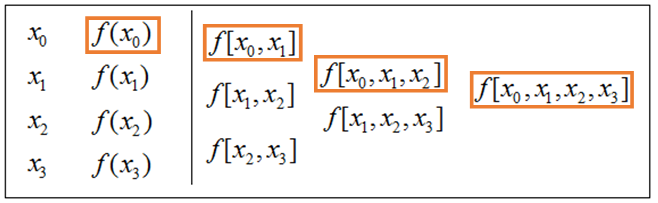
\includegraphics[width=0.55\linewidth]{img06/w06-DividedDifferenceTable} \end{center}

\textbf{Example 1}: Calculate all divided differences based on the following given data table

\begin{longtable}[]{@{}lllll@{}}
\toprule\noalign{}
\(x\) & 3 & 1 & 5 & 6 \\
\midrule\noalign{}
\endhead
\bottomrule\noalign{}
\endlastfoot
\(f(x)\) & 1 & -3 & 2 & 4 \\
\end{longtable}

Based definition, the divided differences are calculated and summarized in the following table.

\begin{center}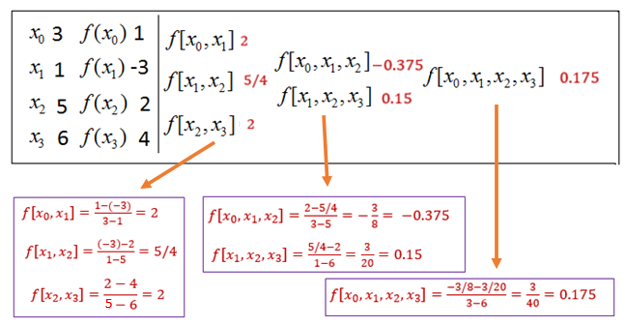
\includegraphics[width=0.7\linewidth]{img06/w06-DividedDifferenceTableExample} \end{center}

\hypertarget{algorithm-of-calculating-divided-differences}{%
\subsection{Algorithm of Calculating Divided Differences}\label{algorithm-of-calculating-divided-differences}}

We re-organize the above calculation in the following matrix and use the logic to develop the pseudo-code for calculating the divided differences.

\begin{center}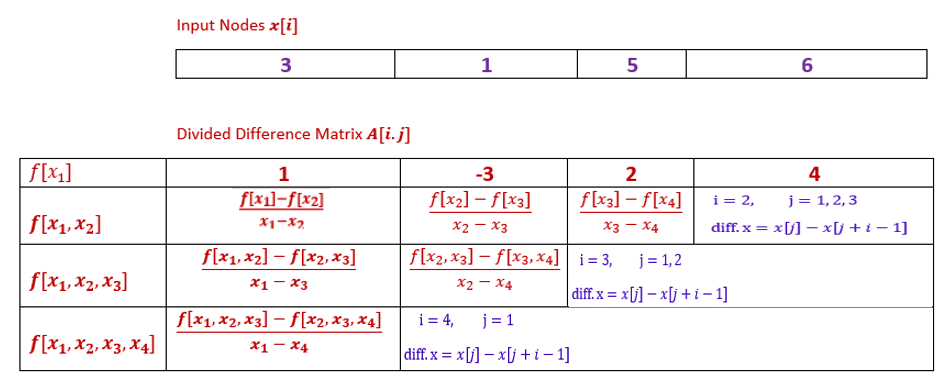
\includegraphics[width=0.95\linewidth]{img06/w06-codingLogic} \end{center}

\textbf{Divided Algorithm}

\begin{verbatim}
INPUT: vec.x              (nodes)
       vec.y (or fn() )
       pred.x
       
OUTPUT: pn(pred.x)

STEP 1: Define a square zero matrix (array): A
STEP 2: Store vec.y in the first row of A
STEP 3: FOR i from 2 to ncol DO:      (Caution: 2nd row!)
            FOR j from 1 to (ncol - i + 1) DO:
                denominator = vec.x[j] - vec.x[j+i-1]
                numerator = A[i-1,j] - A[i-1, j+1]      (using previous row of A)
                A[i,j] = numerator / denominator        (next order divided difference)
            ENDFOR
        ENDFOR
STEP 4: RETURN A
\end{verbatim}

\begin{Shaded}
\begin{Highlighting}[]
\NormalTok{Divided.Dif }\OtherTok{=} \ControlFlowTok{function}\NormalTok{(}
\NormalTok{        vec.x,          }\CommentTok{\# input nodes:}
        \AttributeTok{vec.y =} \ConstantTok{NULL}\NormalTok{,   }\CommentTok{\# one of vec.y and fn must be given}
        \AttributeTok{fn =} \ConstantTok{NULL}\NormalTok{,}
\NormalTok{        pred.x          }\CommentTok{\# scalar x for predicting pn(pred.x)}
\NormalTok{         )\{}
\NormalTok{   n }\OtherTok{=} \FunctionTok{length}\NormalTok{(vec.x)}
   \ControlFlowTok{if}\NormalTok{ (}\FunctionTok{length}\NormalTok{(vec.y) }\SpecialCharTok{==} \DecValTok{0}\NormalTok{) vec.y }\OtherTok{=} \FunctionTok{fn}\NormalTok{(vec.x) }\CommentTok{\#}
\NormalTok{   node.x }\OtherTok{=}\NormalTok{ vec.x}
\NormalTok{   A }\OtherTok{=} \FunctionTok{matrix}\NormalTok{(}\FunctionTok{c}\NormalTok{(}\FunctionTok{rep}\NormalTok{(}\DecValTok{0}\NormalTok{,n}\SpecialCharTok{\^{}}\DecValTok{2}\NormalTok{)), }\AttributeTok{nrow =}\NormalTok{ n, }\AttributeTok{ncol =}\NormalTok{ n, }\AttributeTok{byrow =} \ConstantTok{TRUE}\NormalTok{)}
\NormalTok{   A[}\DecValTok{1}\NormalTok{,] }\OtherTok{=}\NormalTok{ vec.y     }\CommentTok{\# fill the first row with vec.y}
   \CommentTok{\#}
   \ControlFlowTok{for}\NormalTok{(i }\ControlFlowTok{in} \DecValTok{2}\SpecialCharTok{:}\NormalTok{(n))\{}
     \ControlFlowTok{for}\NormalTok{(j }\ControlFlowTok{in} \DecValTok{1}\SpecialCharTok{:}\NormalTok{(n}\SpecialCharTok{{-}}\NormalTok{i}\SpecialCharTok{+}\DecValTok{1}\NormalTok{))\{}
\NormalTok{      denominator }\OtherTok{=}\NormalTok{ vec.x[j] }\SpecialCharTok{{-}}\NormalTok{ vec.x[j}\SpecialCharTok{+}\DecValTok{1}\SpecialCharTok{+}\NormalTok{(i}\DecValTok{{-}2}\NormalTok{)]}
\NormalTok{      numerator }\OtherTok{=}\NormalTok{ A[i}\DecValTok{{-}1}\NormalTok{,j]}\SpecialCharTok{{-}}\NormalTok{ A[i}\DecValTok{{-}1}\NormalTok{,j}\SpecialCharTok{+}\DecValTok{1}\NormalTok{]}
\NormalTok{      A[i,j] }\OtherTok{=}\NormalTok{ numerator}\SpecialCharTok{/}\NormalTok{denominator}
\NormalTok{      \}}
\NormalTok{    \}}
\NormalTok{  A}
\NormalTok{ \}}
\end{Highlighting}
\end{Shaded}

\begin{Shaded}
\begin{Highlighting}[]
\FunctionTok{pander}\NormalTok{(}\FunctionTok{Divided.Dif}\NormalTok{(}
        \AttributeTok{vec.x =} \FunctionTok{c}\NormalTok{(}\DecValTok{3}\NormalTok{,}\DecValTok{1}\NormalTok{,}\DecValTok{5}\NormalTok{,}\DecValTok{6}\NormalTok{),    }\CommentTok{\# input nodes:}
        \AttributeTok{vec.y =} \FunctionTok{c}\NormalTok{(}\DecValTok{1}\NormalTok{,}\SpecialCharTok{{-}}\DecValTok{3}\NormalTok{,}\DecValTok{2}\NormalTok{,}\DecValTok{4}\NormalTok{),   }\CommentTok{\# one of vec.y and fn must be given}
        \AttributeTok{fn =} \ConstantTok{NULL}
\NormalTok{        )}
\NormalTok{)}
\end{Highlighting}
\end{Shaded}

\begin{longtable}[]{@{}
  >{\centering\arraybackslash}p{(\columnwidth - 6\tabcolsep) * \real{0.1250}}
  >{\centering\arraybackslash}p{(\columnwidth - 6\tabcolsep) * \real{0.0972}}
  >{\centering\arraybackslash}p{(\columnwidth - 6\tabcolsep) * \real{0.0556}}
  >{\centering\arraybackslash}p{(\columnwidth - 6\tabcolsep) * \real{0.0556}}@{}}
\toprule\noalign{}
\endhead
\bottomrule\noalign{}
\endlastfoot
1 & -3 & 2 & 4 \\
2 & 1.25 & 2 & 0 \\
-0.375 & 0.15 & 0 & 0 \\
0.175 & 0 & 0 & 0 \\
\end{longtable}

\textbf{Example 2}: (Example 1 of Burden and Faires' textbook, 9th edition, page 127) Complete the divided difference table for the following data.

\begin{longtable}[]{@{}
  >{\raggedright\arraybackslash}p{(\columnwidth - 2\tabcolsep) * \real{0.0556}}
  >{\centering\arraybackslash}p{(\columnwidth - 2\tabcolsep) * \real{0.1389}}@{}}
\toprule\noalign{}
\begin{minipage}[b]{\linewidth}\raggedright
x
\end{minipage} & \begin{minipage}[b]{\linewidth}\centering
y
\end{minipage} \\
\midrule\noalign{}
\endhead
\bottomrule\noalign{}
\endlastfoot
1.0
1.3
1.6
1.9
2.2 & 0.7651977
0.6200860
0.4554022
0.2818186
0.1103623 \\
\end{longtable}

We use the above function to calculate the divided differences.

\begin{Shaded}
\begin{Highlighting}[]
\FunctionTok{pander}\NormalTok{(}\FunctionTok{Divided.Dif}\NormalTok{(}
        \AttributeTok{vec.x =} \FunctionTok{c}\NormalTok{(}\DecValTok{1}\NormalTok{, }\FloatTok{1.3}\NormalTok{, }\FloatTok{1.6}\NormalTok{, }\FloatTok{1.9}\NormalTok{, }\FloatTok{2.2}\NormalTok{),           }
        \AttributeTok{vec.y =} \FunctionTok{c}\NormalTok{(}\FloatTok{0.7651977}\NormalTok{, }\FloatTok{0.6200860}\NormalTok{, }\FloatTok{0.4554022}\NormalTok{, }\FloatTok{0.2818186}\NormalTok{, }\FloatTok{0.1103623}\NormalTok{),    }
        \AttributeTok{fn =} \ConstantTok{NULL}
\NormalTok{        )}
\NormalTok{     )}
\end{Highlighting}
\end{Shaded}

\begin{longtable}[]{@{}
  >{\centering\arraybackslash}p{(\columnwidth - 8\tabcolsep) * \real{0.1528}}
  >{\centering\arraybackslash}p{(\columnwidth - 8\tabcolsep) * \real{0.1528}}
  >{\centering\arraybackslash}p{(\columnwidth - 8\tabcolsep) * \real{0.1389}}
  >{\centering\arraybackslash}p{(\columnwidth - 8\tabcolsep) * \real{0.1389}}
  >{\centering\arraybackslash}p{(\columnwidth - 8\tabcolsep) * \real{0.1389}}@{}}
\toprule\noalign{}
\endhead
\bottomrule\noalign{}
\endlastfoot
0.7652 & 0.6201 & 0.4554 & 0.2818 & 0.1104 \\
-0.4837 & -0.5489 & -0.5786 & -0.5715 & 0 \\
-0.1087 & -0.04944 & 0.01182 & 0 & 0 \\
0.06588 & 0.06807 & 0 & 0 & 0 \\
0.001825 & 0 & 0 & 0 & 0 \\
\end{longtable}

The resulting table is the same as the one obtained in the table of the textbook (except for rounding errors).

\hfill\break

\hypertarget{newton-interpolation-polynomial}{%
\section{Newton Interpolation Polynomial}\label{newton-interpolation-polynomial}}

From the definition of the divided difference, for any \(x\) and \(x_0\), we have

\[
f[x,x_0] = \frac{f(x)-f(x_0)}{x-x_0}
\]

Solving for \(f(x)\), we have

\[
f(x) = f(x_0) + f[x, x_0](x - x_0).
\]

Similarly, for \(x_0\) and \(x_1\), the second order divided difference is given by

\[
f[x,x_0, x_1] = \frac{f[x, x_0]-f[x_0,x_1]}{x-x_1}
\]

Therefore,

\[
f[x,x_0] = f[x_0,x_1] + f[x, x_0, x_1](x - x_1).
\]
That is,

\[
f(x) = f[x_0] + f[x_0, x_1](x - x_0)  + f[x, x_0, x_1](x - x_0)(x - x_1).
\]

Repeating the above calculation, we have

\[
f(x) = f[x_0] + f[x_0, x_1](x-x_0) + f[x_0, x_1, x_2](x-x_0)(x-x_1) + \cdots + f[x, x_0, \cdots, x_n](x-x_0)\cdots(x-x_{n-1})
\]

\hypertarget{definition-of-newton-interpolation}{%
\subsection{Definition of Newton Interpolation}\label{definition-of-newton-interpolation}}

Based on the above derivation, we define \textbf{Newton Form Interpolation Polynomial} to be of the following form

\[
N_n(x) = f[x_0] + f[x_0, x_1](x-x_0) + f[x_0, x_1, x_2](x-x_0)(x-x_1) + \cdots + f[x_0, \cdots, x_n](x-x_0)\cdots(x-x_{n-1})
\]

We can see that \(N_n(x)\) passes all interpolating points:

\[
N_n(x_0) = f(x_0)
\]

\[
N_n(x_1) = f(x_0) + f[x_0, x_1](x_1-x_0) = f(x_0) + \frac{f(x_1)-f(x_0)}{x_1-x_0}(x_1-x_0) = f(x_1)
\]
In general,

\[
N_n(x_k) = f(x_k), \ \ \text{ for } \ \ 0 \le k \le n.
\]

\hypertarget{newton-interpolation-algorithm}{%
\subsection{Newton Interpolation Algorithm}\label{newton-interpolation-algorithm}}

The associated \textbf{divided differences} in the above \textbf{Newton Interpolation Polynomial} are returned in the first column of the function \texttt{Divided.Dif()}. To write the algorithmic function

\textbf{Newton Interpolation Algorithm 2}

\begin{verbatim}
INPUT:  vec.x
        vec.y or fn
        pred.x     (for prediction)
OUTPUT: pred.y     (pn(pred.x))

STEP 1: initialization:
        Divided.Dif          (function call)
        Pn = 0
        
STEP 2: FOR i from 1 to n DO:
          cumProd = 1             (initial value for the cumulative product)
          FOR j from 1 to i DO:
              cumProd = cumProd*(pred.x-vec.x[j])
          ENDFOR
          Pn = Pn + Divided.Dif[i]*cumProd
        ENDFOR
STEP 3: RETURN(Pn)
\end{verbatim}

Next, we write an R function to implement the Newton interpolation polynomial.

\begin{Shaded}
\begin{Highlighting}[]
\NormalTok{NewtonInterpolation }\OtherTok{=} \ControlFlowTok{function}\NormalTok{( vec.x,            }\CommentTok{\# input interpolation nodes}
                                \AttributeTok{vec.y =} \ConstantTok{NULL}\NormalTok{,    }
                                \AttributeTok{fn =} \ConstantTok{NULL}\NormalTok{,        }\CommentTok{\# either vec.y or fn must be provided}
\NormalTok{                                pred.x            }\CommentTok{\# single value of x for prediction}
\NormalTok{                              )\{}
   \ControlFlowTok{if}\NormalTok{(}\FunctionTok{length}\NormalTok{(vec.y) }\SpecialCharTok{==}\DecValTok{0}\NormalTok{) vec.y }\OtherTok{=} \FunctionTok{fn}\NormalTok{(vec.x)}
\NormalTok{   DivDif }\OtherTok{=} \FunctionTok{Divided.Dif}\NormalTok{(vec.x, vec.y)[,}\DecValTok{1}\NormalTok{]       }\CommentTok{\# the values in the first column of the div dif matrix}
\NormalTok{   n }\OtherTok{=} \FunctionTok{length}\NormalTok{(vec.x)}
\NormalTok{   Nn }\OtherTok{=}\NormalTok{ vec.y[}\DecValTok{1}\NormalTok{]                  }\CommentTok{\# f[xo]}
   \ControlFlowTok{for}\NormalTok{ (i }\ControlFlowTok{in} \DecValTok{1}\SpecialCharTok{:}\NormalTok{(n}\DecValTok{{-}1}\NormalTok{))\{            }\CommentTok{\# Must be n {-} 1 according to the last term in the polynomial}
\NormalTok{     cumProd }\OtherTok{=} \DecValTok{1}                  \CommentTok{\# initial value to calculate the cumulative product}
     \ControlFlowTok{for}\NormalTok{(j }\ControlFlowTok{in} \DecValTok{1}\SpecialCharTok{:}\NormalTok{i)\{               }\CommentTok{\# forward difference formula}
\NormalTok{       cumProd }\OtherTok{=}\NormalTok{ cumProd}\SpecialCharTok{*}\NormalTok{(pred.x}\SpecialCharTok{{-}}\NormalTok{vec.x[j])   }\CommentTok{\# updating the cumulative product in the inner loop}
\NormalTok{     \}}
\NormalTok{     Nn }\OtherTok{=}\NormalTok{ Nn }\SpecialCharTok{+}\NormalTok{ DivDif[i}\SpecialCharTok{+}\DecValTok{1}\NormalTok{]}\SpecialCharTok{*}\NormalTok{cumProd    }\CommentTok{\# adding high order terms alliteratively to the Nn(x) }
\NormalTok{   \}}
\NormalTok{  Nn                                  }\CommentTok{\# return the value of the Newton polynomial}
\NormalTok{\}}
\end{Highlighting}
\end{Shaded}

\textbf{Example 3} (Continuation of \emph{example 2}). We evaluate the Newton interpolation polynomial \(p_4(x)\) at \(x = 1.1, 1.6\) and \(2.0\), respectively. Recall the given data points are

\begin{longtable}[]{@{}
  >{\raggedright\arraybackslash}p{(\columnwidth - 2\tabcolsep) * \real{0.0556}}
  >{\centering\arraybackslash}p{(\columnwidth - 2\tabcolsep) * \real{0.1389}}@{}}
\toprule\noalign{}
\begin{minipage}[b]{\linewidth}\raggedright
x
\end{minipage} & \begin{minipage}[b]{\linewidth}\centering
y
\end{minipage} \\
\midrule\noalign{}
\endhead
\bottomrule\noalign{}
\endlastfoot
1.0
1.3
1.6
1.9
2.2 & 0.7651977
0.6200860
0.4554022
0.2818186
0.1103623 \\
\end{longtable}

\textbf{Solution}: We use the above R function to evaluate the function at the two given nodes.

\begin{Shaded}
\begin{Highlighting}[]
\NormalTok{pred.}\FloatTok{1.6} \OtherTok{=} \FunctionTok{NewtonInterpolation}\NormalTok{(}\AttributeTok{vec.x =} \FunctionTok{c}\NormalTok{(}\DecValTok{1}\NormalTok{, }\FloatTok{1.3}\NormalTok{, }\FloatTok{1.6}\NormalTok{, }\FloatTok{1.9}\NormalTok{, }\FloatTok{2.2}\NormalTok{),           }
                    \AttributeTok{vec.y =} \FunctionTok{c}\NormalTok{(}\FloatTok{0.7651977}\NormalTok{, }\FloatTok{0.6200860}\NormalTok{, }\FloatTok{0.4554022}\NormalTok{, }\FloatTok{0.2818186}\NormalTok{, }\FloatTok{0.1103623}\NormalTok{), }
                    \AttributeTok{pred.x =} \FloatTok{1.6}\NormalTok{)}
\NormalTok{pred.}\FloatTok{1.1} \OtherTok{=} \FunctionTok{NewtonInterpolation}\NormalTok{(}\AttributeTok{vec.x =} \FunctionTok{c}\NormalTok{(}\DecValTok{1}\NormalTok{, }\FloatTok{1.3}\NormalTok{, }\FloatTok{1.6}\NormalTok{, }\FloatTok{1.9}\NormalTok{, }\FloatTok{2.2}\NormalTok{),           }
                    \AttributeTok{vec.y =} \FunctionTok{c}\NormalTok{(}\FloatTok{0.7651977}\NormalTok{, }\FloatTok{0.6200860}\NormalTok{, }\FloatTok{0.4554022}\NormalTok{, }\FloatTok{0.2818186}\NormalTok{, }\FloatTok{0.1103623}\NormalTok{), }
                    \AttributeTok{pred.x =} \FloatTok{1.1}\NormalTok{)}
\NormalTok{pred.}\FloatTok{2.0} \OtherTok{=} \FunctionTok{NewtonInterpolation}\NormalTok{(}\AttributeTok{vec.x =} \FunctionTok{c}\NormalTok{(}\DecValTok{1}\NormalTok{, }\FloatTok{1.3}\NormalTok{, }\FloatTok{1.6}\NormalTok{, }\FloatTok{1.9}\NormalTok{, }\FloatTok{2.2}\NormalTok{),           }
                    \AttributeTok{vec.y =} \FunctionTok{c}\NormalTok{(}\FloatTok{0.7651977}\NormalTok{, }\FloatTok{0.6200860}\NormalTok{, }\FloatTok{0.4554022}\NormalTok{, }\FloatTok{0.2818186}\NormalTok{, }\FloatTok{0.1103623}\NormalTok{), }
                    \AttributeTok{pred.x =} \FloatTok{2.0}\NormalTok{)}

\FunctionTok{pander}\NormalTok{(}\FunctionTok{cbind}\NormalTok{(}\AttributeTok{pred.1.6=}\NormalTok{pred.}\FloatTok{1.6}\NormalTok{, }\AttributeTok{pred.1.1=}\NormalTok{pred.}\FloatTok{1.1}\NormalTok{, }\AttributeTok{pred.2.0 =}\NormalTok{ pred.}\FloatTok{2.0}\NormalTok{))}
\end{Highlighting}
\end{Shaded}

\begin{longtable}[]{@{}
  >{\centering\arraybackslash}p{(\columnwidth - 4\tabcolsep) * \real{0.1528}}
  >{\centering\arraybackslash}p{(\columnwidth - 4\tabcolsep) * \real{0.1528}}
  >{\centering\arraybackslash}p{(\columnwidth - 4\tabcolsep) * \real{0.1528}}@{}}
\toprule\noalign{}
\begin{minipage}[b]{\linewidth}\centering
pred.1.6
\end{minipage} & \begin{minipage}[b]{\linewidth}\centering
pred.1.1
\end{minipage} & \begin{minipage}[b]{\linewidth}\centering
pred.2.0
\end{minipage} \\
\midrule\noalign{}
\endhead
\bottomrule\noalign{}
\endlastfoot
0.4554 & 0.7196 & 0.2239 \\
\end{longtable}

The results are the same as those obtained in the textbook Burden and Faires (9th edition, page 131).

\textbf{R Function: Vector Enabled Newton Interpolated Polynomial}

Next, we modify the previous R function to take a vector of input x-values for prediction just like other R functions.

\begin{Shaded}
\begin{Highlighting}[]
\DocumentationTok{\#\#\#\#\#\#\#\#\#\#\#\#\#\#\#\#\#\#\#\#\#\#\#\#\#\#\#\#\#\#\#\#\#\#\#\#\#\#\#\#\#\#\#\#\#\#\#\#\#\#\#\#\#\#\#\#\#\#\#\#\#\#\#\#\#\#\#\#\#\#\#\#\#\#\#\#\#\#\#\#\#\#}
\DocumentationTok{\#\#  Newton Interpolated Polynomial Approximation: vector{-}enabled input}
\DocumentationTok{\#\#\#\#\#\#\#\#\#\#\#\#\#\#\#\#\#\#\#\#\#\#\#\#\#\#\#\#\#\#\#\#\#\#\#\#\#\#\#\#\#\#\#\#\#\#\#\#\#\#\#\#\#\#\#\#\#\#\#\#\#\#\#\#\#\#\#\#\#\#\#\#\#\#\#\#\#\#\#\#\#\#}

\NormalTok{Newton.Interpolation }\OtherTok{=} \ControlFlowTok{function}\NormalTok{( vec.x,            }\CommentTok{\# input interpolation nodes}
                                \AttributeTok{vec.y =} \ConstantTok{NULL}\NormalTok{,    }
                                \AttributeTok{fn =} \ConstantTok{NULL}\NormalTok{,        }\CommentTok{\# either vec.y or fn must be provided}
\NormalTok{                                pred.x            }\CommentTok{\# VECTOR INPUT!!!}
\NormalTok{                              )\{}
   \ControlFlowTok{if}\NormalTok{(}\FunctionTok{length}\NormalTok{(vec.y) }\SpecialCharTok{==}\DecValTok{0}\NormalTok{) vec.y }\OtherTok{=} \FunctionTok{fn}\NormalTok{(vec.x)}
\NormalTok{   DivDif }\OtherTok{=} \FunctionTok{Divided.Dif}\NormalTok{(vec.x, vec.y)[,}\DecValTok{1}\NormalTok{]       }\CommentTok{\# the values in the first column of the div dif matrix}
\NormalTok{   n }\OtherTok{=} \FunctionTok{length}\NormalTok{(vec.x)}
   \DocumentationTok{\#\#\#\#\#\#\#\#\#\#\#\#}
\NormalTok{   m }\OtherTok{=} \FunctionTok{length}\NormalTok{(pred.x)}
\NormalTok{   NV }\OtherTok{=} \FunctionTok{rep}\NormalTok{(}\DecValTok{0}\NormalTok{, m)                 }\CommentTok{\# values of Nn(pred.x)}
   \ControlFlowTok{for}\NormalTok{(k }\ControlFlowTok{in} \DecValTok{1}\SpecialCharTok{:}\NormalTok{m) \{}
   \DocumentationTok{\#\#\#\#\#\#\#\#\#\#\#\#\#\#\#\#}
\NormalTok{   Nn }\OtherTok{=}\NormalTok{ vec.y[}\DecValTok{1}\NormalTok{]                  }\CommentTok{\# f[xo]}
   \ControlFlowTok{for}\NormalTok{ (i }\ControlFlowTok{in} \DecValTok{1}\SpecialCharTok{:}\NormalTok{(n}\DecValTok{{-}1}\NormalTok{))\{            }\CommentTok{\# Must be n {-} 1 according to the last term in the polynomial}
\NormalTok{     cumProd }\OtherTok{=} \DecValTok{1}                  \CommentTok{\# initial value to calculate the cumulative product}
     \ControlFlowTok{for}\NormalTok{(j }\ControlFlowTok{in} \DecValTok{1}\SpecialCharTok{:}\NormalTok{i)\{               }\CommentTok{\# forward difference formula}
\NormalTok{       cumProd }\OtherTok{=}\NormalTok{ cumProd}\SpecialCharTok{*}\NormalTok{(pred.x[k]}\SpecialCharTok{{-}}\NormalTok{vec.x[j])   }\CommentTok{\# updating the cumulative product in the inner loop}
\NormalTok{     \}}
\NormalTok{      Nn }\OtherTok{=}\NormalTok{ Nn }\SpecialCharTok{+}\NormalTok{ DivDif[i}\SpecialCharTok{+}\DecValTok{1}\NormalTok{]}\SpecialCharTok{*}\NormalTok{cumProd    }\CommentTok{\# adding high order terms alliteratively to the Nn(x) }
\NormalTok{    \}}
\NormalTok{    NV[k] }\OtherTok{=}\NormalTok{ Nn                                  }\CommentTok{\# return the value the Newton polynomial}
\NormalTok{   \}}
\NormalTok{ NV  }
\NormalTok{\}}
\end{Highlighting}
\end{Shaded}

\begin{Shaded}
\begin{Highlighting}[]
\NormalTok{pred.x }\OtherTok{=} \FunctionTok{c}\NormalTok{(}\FloatTok{1.6}\NormalTok{, }\FloatTok{1.1}\NormalTok{, }\FloatTok{2.0}\NormalTok{)   }\CommentTok{\# pred.x is the argument is a local variable!}
\NormalTok{pred.NIP }\OtherTok{=} \FunctionTok{Newton.Interpolation}\NormalTok{(}\AttributeTok{vec.x =} \FunctionTok{c}\NormalTok{(}\DecValTok{1}\NormalTok{, }\FloatTok{1.3}\NormalTok{, }\FloatTok{1.6}\NormalTok{, }\FloatTok{1.9}\NormalTok{, }\FloatTok{2.2}\NormalTok{),           }
                    \AttributeTok{vec.y =} \FunctionTok{c}\NormalTok{(}\FloatTok{0.7651977}\NormalTok{, }\FloatTok{0.6200860}\NormalTok{, }\FloatTok{0.4554022}\NormalTok{, }\FloatTok{0.2818186}\NormalTok{, }\FloatTok{0.1103623}\NormalTok{), }
                    \AttributeTok{pred.x =} \FunctionTok{c}\NormalTok{(}\FloatTok{1.6}\NormalTok{, }\FloatTok{1.1}\NormalTok{, }\FloatTok{2.0}\NormalTok{))}
\FunctionTok{pander}\NormalTok{(}\FunctionTok{cbind}\NormalTok{(}\AttributeTok{pred.x =}\NormalTok{ pred.x, }\AttributeTok{pred.NIP=}\NormalTok{pred.NIP))}
\end{Highlighting}
\end{Shaded}

\begin{longtable}[]{@{}
  >{\centering\arraybackslash}p{(\columnwidth - 2\tabcolsep) * \real{0.1250}}
  >{\centering\arraybackslash}p{(\columnwidth - 2\tabcolsep) * \real{0.1528}}@{}}
\toprule\noalign{}
\begin{minipage}[b]{\linewidth}\centering
pred.x
\end{minipage} & \begin{minipage}[b]{\linewidth}\centering
pred.NIP
\end{minipage} \\
\midrule\noalign{}
\endhead
\bottomrule\noalign{}
\endlastfoot
1.6 & 0.4554 \\
1.1 & 0.7196 \\
2 & 0.2239 \\
\end{longtable}

\hypertarget{error-analysis-6}{%
\section{Error Analysis}\label{error-analysis-6}}

Using the generalized Rolle theorem repeatedly on the expression of the divided difference, have the following result.

\textbf{Theorem}: Let \(x_0, \cdots , x_{n-1}\), \(x\) be \(n+1\) distinct points. Let \(a = \min (x_0, \cdots , x_{n-1}, x)\) and \(b = \max(x_0, \cdots , x_{n-1},x)\). Assume that \(f(x)\) has a continuous derivative of order \(n\) in the interval \((a, b)\). Then

\[
f[x_0, x_1, \cdots, x_{n-1}, x] = \frac{f^{(n)}(\xi)}{n!}
\]

where \(\xi \in (a, b)\).

\textbf{Proof}: Let \(P_{n+1}(y)\) be the interpolated polynomial at \(y\) for given nodes \(\{ x_0, x_1, x_2, \cdots, x_{n-1},x \}\) such that \(P_{n+1}(x_i) = f(x_i)\) for \(i = 0, 1, 2, \cdots, n-1\), and \(P_{n+1}(x) = f(x)\). From the construction of Newton interpolating polynomial \(P_n(x)\), we know that
\[
P_n(y) = P_{n-1}(x) + f[x_0, x_1, x_2, \cdots, x_{n-1},x] (x-x_0)\cdots(x-x_{n-1})
\]
Apparently,

\[
f(x) =P_n(x) = P_{n-1}(x) + f[x0, x1, x2, \cdots, x_{n-1},x] (x-x_0)\cdots(x-x_{n-1})
\]
Using the theorem introduced in the last unit and the uniqueness of the app, we have

\[
f(x) = P_{n-1}(x) + \frac{f^{(n)}(\xi)}{n!}(x-x_0)(x-x_1)\cdots(x-x_{n-1}).
\]

Using the same arguments in the Lagrange interpolation polynomial, we can establish the error bound for the Newton form interpolation polynomials.

\hypertarget{some-remarks-of-newton-interpolation}{%
\section{Some Remarks of Newton Interpolation}\label{some-remarks-of-newton-interpolation}}

First of all, both Lagrange and Newton interpolation polynomials introduced earlier can be viewed as a linear combination of basis polynomials \(\{x^0, x^1, x^2, x^2, \cdots, x^n \}\). In fact, Lagrange and Newton interpolation polynomials are two different algebraic representations of the same polynomial.

That is, \(P_n(x)\) and \(N_n(x)\) be Lagrange and Newton interpolation polynomials based on \((x_0, y_0), (x_1, y_1), (x_2, y_2), \cdots, (x_n, y_n)\). We express both \(P_n(x)\) and \(N_n(x)\) in terms of basis polynomials \(\{x^0, x^1, x^2, x^2, \cdots, x^n \}\) as

\[
P_n(x) = a_0 + a_1x + a_2x^2 + \cdots + a_nx^n \ \ \text{ and } \ \ N_n(x) = b_0 + b_1x + b_2x^2 + \cdots + b_nx^n
\]
Since \(P_n(x_i) = y_i = N_n(x_i)\) for \(i = x_0, x_1, \cdots, x_n\), we can easily show that \(a_j = b_j\) for \(j = 0, 1, 2, \cdots, n\). Therefore, the error bounds of both Lagrange and Newton interpolation polynomials are the same.

For the Newton form interpolation polynomial, we only need to add more terms if additional interpolation nodes are added to the existing ones. Since the divided differences are independent of the newly added nodes. But for the Lagrange form, we need to restart the program. This is a unique feature of the Newton interpolation polynomial.

\textbf{Example 4}. Use the Newton Interpolation polynomial to approximate \(f(x) = \sin(x)\) with interpolating nodes \(x = -\pi, -0.75\pi, -0.5\pi, 0.25\pi, 0, 0.25\pi, 0.5\pi, 0.75\pi, \pi\).

\textbf{Solution}: We plot both \(f(x) = \sin(x)\) and \(N_8(x)\) over interval \([-2\pi, 2\pi]\) and see the performance of the approximation.

\begin{Shaded}
\begin{Highlighting}[]
\NormalTok{nodes }\OtherTok{=} \FunctionTok{c}\NormalTok{(}\SpecialCharTok{{-}}\FloatTok{1.5}\SpecialCharTok{*}\NormalTok{pi, }\SpecialCharTok{{-}}\NormalTok{pi, }\SpecialCharTok{{-}}\FloatTok{0.5}\SpecialCharTok{*}\NormalTok{pi, }\SpecialCharTok{{-}}\FloatTok{0.25}\SpecialCharTok{*}\NormalTok{pi, }\DecValTok{0}\NormalTok{, }\FloatTok{0.25}\SpecialCharTok{*}\NormalTok{pi, }\FloatTok{0.5}\SpecialCharTok{*}\NormalTok{pi,  pi, }\FloatTok{1.5}\SpecialCharTok{*}\NormalTok{pi)}
\DocumentationTok{\#\#\#\#}
\NormalTok{xx }\OtherTok{=} \FunctionTok{seq}\NormalTok{(}\SpecialCharTok{{-}}\DecValTok{2}\SpecialCharTok{*}\NormalTok{pi, }\DecValTok{2}\SpecialCharTok{*}\NormalTok{pi, }\AttributeTok{length =} \DecValTok{50}\NormalTok{)}
\NormalTok{yy }\OtherTok{=} \FunctionTok{sin}\NormalTok{(xx)}
\NormalTok{Nn }\OtherTok{=} \FunctionTok{Newton.Interpolation}\NormalTok{(}\AttributeTok{vec.x =}\NormalTok{ nodes,           }
                    \AttributeTok{vec.y =} \FunctionTok{sin}\NormalTok{(nodes), }
                    \AttributeTok{pred.x =}\NormalTok{ xx)}
\FunctionTok{plot}\NormalTok{(xx, Nn, }\AttributeTok{xlab =} \StringTok{""}\NormalTok{, }\AttributeTok{ylab =} \StringTok{""}\NormalTok{, }\AttributeTok{type =} \StringTok{"l"}\NormalTok{, }\AttributeTok{lwd =} \DecValTok{2}\NormalTok{, }\AttributeTok{col =} \StringTok{"red"}\NormalTok{, }\AttributeTok{ylim =} \FunctionTok{c}\NormalTok{(}\SpecialCharTok{{-}}\DecValTok{2}\NormalTok{,}\DecValTok{2}\NormalTok{), }
         \AttributeTok{main =} \StringTok{"Newton Interpolation Polynomial"}\NormalTok{)}
\FunctionTok{lines}\NormalTok{(xx, yy, }\AttributeTok{lty =}\DecValTok{2}\NormalTok{, }\AttributeTok{col =} \StringTok{"blue"}\NormalTok{, }\AttributeTok{lwd =} \DecValTok{2}\NormalTok{)}
\FunctionTok{abline}\NormalTok{(}\AttributeTok{h =} \DecValTok{0}\NormalTok{, }\AttributeTok{lty =} \DecValTok{2}\NormalTok{, }\AttributeTok{col =} \StringTok{"purple"}\NormalTok{)}
\end{Highlighting}
\end{Shaded}

\begin{center}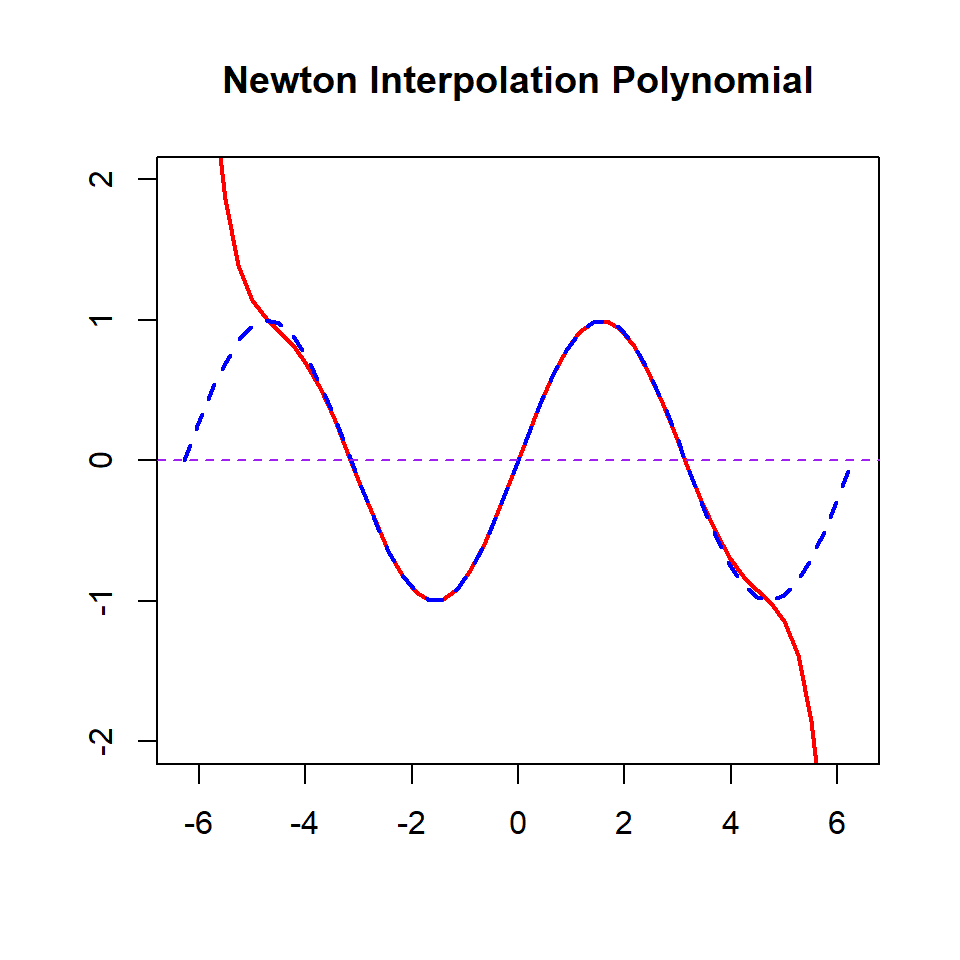
\includegraphics{MAT325EB_files/figure-latex/unnamed-chunk-103-1} \end{center}

\hypertarget{implicit-loops-in-r-programming}{%
\section{Implicit Loops in R Programming}\label{implicit-loops-in-r-programming}}

This lab note introduces how to reduce loops through vectorization. For any vectorized language, there are different extensions such as user-defined functions and routines to carry vectorized operation instead of element-wise operation. Most R functions are vectorized. We will use some examples to illustrate how a loop can be avoided if vectorization is available.

\hfill\break

\hypertarget{implicit-in-r-primitive-functions}{%
\subsection{Implicit in R Primitive Functions}\label{implicit-in-r-primitive-functions}}

R was written in C. It has a long list of primitive functions written in C. Most of these functions are vectorized. Calling an internal vectorized function is the same as performing an implicit loop.

\textbf{Example 1}: Consider the sum of two matrices with the same dimension. Define

\[
A = \begin{pmatrix}
1 & 2 & 3\\
3 & 7 & 9
\end{pmatrix}
\]

and

\[
B = \begin{pmatrix}
5 & 2 & 7\\
4 & 1 & 6
\end{pmatrix}
\]

We find the sum of \(A\) and \(B\)

\[
A + B = \begin{pmatrix}
6 & 4 & 10\\
7 & 8 & 15
\end{pmatrix}
\]

\textbf{Method 1}: Using explicit loops. Since the sum of compatible matrices is an element-wise operation, in order to access individual elements, we need to use two indexes - one for the row and one for the column. We use the double loops to calculate the sum of two matrices in the following code.

\begin{Shaded}
\begin{Highlighting}[]
\NormalTok{loopSum }\OtherTok{=} \ControlFlowTok{function}\NormalTok{(A,B)\{}
\NormalTok{    sumAB }\OtherTok{=} \FunctionTok{matrix}\NormalTok{(}\DecValTok{0}\NormalTok{, }\AttributeTok{nrow =} \FunctionTok{dim}\NormalTok{(A)[}\DecValTok{1}\NormalTok{], }\AttributeTok{ncol =} \FunctionTok{dim}\NormalTok{(A)[}\DecValTok{2}\NormalTok{])}
        \ControlFlowTok{for}\NormalTok{(i }\ControlFlowTok{in} \DecValTok{1}\SpecialCharTok{:}\FunctionTok{dim}\NormalTok{(A)[}\DecValTok{1}\NormalTok{]) \{}
            \ControlFlowTok{for}\NormalTok{ (j }\ControlFlowTok{in} \DecValTok{1}\SpecialCharTok{:}\FunctionTok{dim}\NormalTok{(A)[}\DecValTok{2}\NormalTok{])\{}
\NormalTok{                sumAB[i,j] }\OtherTok{=}\NormalTok{ A[i,j] }\SpecialCharTok{+}\NormalTok{ B[i,j]}
\NormalTok{             \}}
\NormalTok{         \}}
\NormalTok{    sumAB}
\NormalTok{ \}}
\end{Highlighting}
\end{Shaded}

We can also use R primitive function \texttt{+} to perform the matrix summation.

\begin{Shaded}
\begin{Highlighting}[]
\NormalTok{vectorSum }\OtherTok{=} \ControlFlowTok{function}\NormalTok{(A,B) \{A }\SpecialCharTok{+}\NormalTok{ B\}}
\end{Highlighting}
\end{Shaded}

\begin{Shaded}
\begin{Highlighting}[]
\NormalTok{A }\OtherTok{=} \FunctionTok{matrix}\NormalTok{(}\FunctionTok{c}\NormalTok{(}\DecValTok{1}\NormalTok{,}\DecValTok{2}\NormalTok{,}\DecValTok{3}\NormalTok{,}\DecValTok{3}\NormalTok{,}\DecValTok{7}\NormalTok{,}\DecValTok{9}\NormalTok{), }\AttributeTok{ncol =} \DecValTok{3}\NormalTok{, }\AttributeTok{byrow =} \ConstantTok{TRUE}\NormalTok{)}
\NormalTok{B }\OtherTok{=} \FunctionTok{matrix}\NormalTok{(}\FunctionTok{c}\NormalTok{(}\DecValTok{5}\NormalTok{,}\DecValTok{2}\NormalTok{,}\DecValTok{7}\NormalTok{,}\DecValTok{4}\NormalTok{,}\DecValTok{1}\NormalTok{,}\DecValTok{6}\NormalTok{), }\AttributeTok{ncol =} \DecValTok{3}\NormalTok{, }\AttributeTok{byrow =} \ConstantTok{TRUE}\NormalTok{)}
\end{Highlighting}
\end{Shaded}

\begin{Shaded}
\begin{Highlighting}[]
\NormalTok{start }\OtherTok{\textless{}{-}} \FunctionTok{Sys.time}\NormalTok{()}
\FunctionTok{loopSum}\NormalTok{(A,B)}
\end{Highlighting}
\end{Shaded}

\begin{verbatim}
##      [,1] [,2] [,3]
## [1,]    6    4   10
## [2,]    7    8   15
\end{verbatim}

\begin{Shaded}
\begin{Highlighting}[]
\FunctionTok{print}\NormalTok{( }\FunctionTok{Sys.time}\NormalTok{() }\SpecialCharTok{{-}}\NormalTok{ start )}
\end{Highlighting}
\end{Shaded}

\begin{verbatim}
## Time difference of 0.01143289 secs
\end{verbatim}

\begin{Shaded}
\begin{Highlighting}[]
\NormalTok{start }\OtherTok{\textless{}{-}} \FunctionTok{Sys.time}\NormalTok{()}
\FunctionTok{vectorSum}\NormalTok{(A,B)}
\end{Highlighting}
\end{Shaded}

\begin{verbatim}
##      [,1] [,2] [,3]
## [1,]    6    4   10
## [2,]    7    8   15
\end{verbatim}

\begin{Shaded}
\begin{Highlighting}[]
\FunctionTok{print}\NormalTok{( }\FunctionTok{Sys.time}\NormalTok{() }\SpecialCharTok{{-}}\NormalTok{ start )}
\end{Highlighting}
\end{Shaded}

\begin{verbatim}
## Time difference of 0.007189035 secs
\end{verbatim}

\textbf{Example 2}: Summation of large matrices.

\begin{Shaded}
\begin{Highlighting}[]
\NormalTok{A0 }\OtherTok{=} \FunctionTok{matrix}\NormalTok{(}\FunctionTok{runif}\NormalTok{(}\DecValTok{10000000}\NormalTok{), }\AttributeTok{ncol =} \DecValTok{5000}\NormalTok{)}
\NormalTok{B0 }\OtherTok{=} \FunctionTok{matrix}\NormalTok{(}\FunctionTok{runif}\NormalTok{(}\DecValTok{10000000}\NormalTok{), }\AttributeTok{ncol =} \DecValTok{5000}\NormalTok{)}
\end{Highlighting}
\end{Shaded}

\begin{Shaded}
\begin{Highlighting}[]
\NormalTok{start }\OtherTok{\textless{}{-}} \FunctionTok{Sys.time}\NormalTok{()}
\NormalTok{AplusB.lp }\OtherTok{=} \FunctionTok{loopSum}\NormalTok{(A0,B0)}
\FunctionTok{print}\NormalTok{( }\FunctionTok{Sys.time}\NormalTok{() }\SpecialCharTok{{-}}\NormalTok{ start )}
\end{Highlighting}
\end{Shaded}

\begin{verbatim}
## Time difference of 1.090455 secs
\end{verbatim}

\begin{Shaded}
\begin{Highlighting}[]
\NormalTok{start }\OtherTok{\textless{}{-}} \FunctionTok{Sys.time}\NormalTok{()}
\NormalTok{AplusB.vec }\OtherTok{=} \FunctionTok{vectorSum}\NormalTok{(A0,B0)}
\FunctionTok{print}\NormalTok{( }\FunctionTok{Sys.time}\NormalTok{() }\SpecialCharTok{{-}}\NormalTok{ start )}
\end{Highlighting}
\end{Shaded}

\begin{verbatim}
## Time difference of 0.1106699 secs
\end{verbatim}

The obvious benefits of using an implicit vectorized primitive function to perform matrix operation:

\begin{enumerate}
\def\labelenumi{\arabic{enumi}.}
\item
  The code is simple.
\item
  It is faster.
\end{enumerate}

\hypertarget{some-vectorized-primitive-functions}{%
\subsection{Some Vectorized Primitive Functions}\label{some-vectorized-primitive-functions}}

Since the numerator and denominator are defined as the difference between adjacent terms. We can vectorize these differences using the R function \textbf{diff()} that computes the difference between pairs of consecutive elements of a numeric vector.

\textbf{Example 2}: Consider \texttt{vec.x\ =\ (1,\ 1.3,\ 1.6,\ 1.9,\ 2.2)} and \texttt{vec.y\ =\ (0.7651977,\ 0.6200860,\ 0.4554022,\ 0.2818186,\ 0.1103623)}. We use the \textbf{diff()} to calculate the divided differences in the following table step by step.

\begin{center}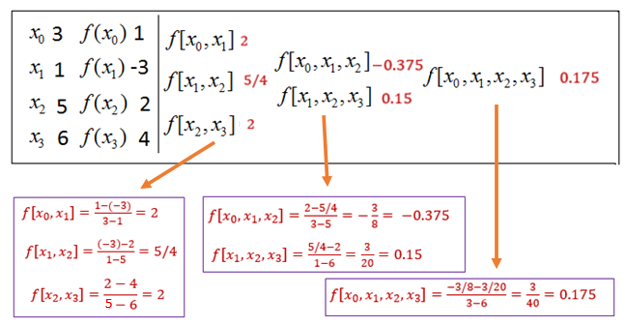
\includegraphics[width=0.7\linewidth]{img06/w06-DividedDifferenceTableExample} \end{center}

The following are manual steps for calculating the divided differences in the above table.

\begin{itemize}
\tightlist
\item
  \emph{Step 1}: zero-th order divided differences (\(i = 1\))
\end{itemize}

\begin{Shaded}
\begin{Highlighting}[]
\NormalTok{vec.x }\OtherTok{=} \FunctionTok{c}\NormalTok{(}\DecValTok{3}\NormalTok{,}\DecValTok{1}\NormalTok{,}\DecValTok{5}\NormalTok{,}\DecValTok{6}\NormalTok{)          }
\NormalTok{vec.y }\OtherTok{=} \FunctionTok{c}\NormalTok{(}\DecValTok{1}\NormalTok{,}\SpecialCharTok{{-}}\DecValTok{3}\NormalTok{,}\DecValTok{2}\NormalTok{,}\DecValTok{4}\NormalTok{)}
\NormalTok{n }\OtherTok{=} \FunctionTok{length}\NormalTok{(vec.x)}
\end{Highlighting}
\end{Shaded}

\begin{itemize}
\tightlist
\item
  \emph{Step 2}: The first order divided differences (i = 2)
\end{itemize}

\begin{Shaded}
\begin{Highlighting}[]
\NormalTok{i}\OtherTok{=}\DecValTok{2}
\DocumentationTok{\#\# divided difference}
\NormalTok{i2.y }\OtherTok{=} \FunctionTok{diff}\NormalTok{(vec.y)}
\NormalTok{i2.x }\OtherTok{=}\NormalTok{ vec.x[}\SpecialCharTok{{-}}\NormalTok{(}\DecValTok{1}\SpecialCharTok{:}\NormalTok{(i}\DecValTok{{-}1}\NormalTok{))] }\SpecialCharTok{{-}}\NormalTok{ vec.x[}\SpecialCharTok{{-}}\NormalTok{((n}\SpecialCharTok{+}\DecValTok{2}\SpecialCharTok{{-}}\NormalTok{i)}\SpecialCharTok{:}\NormalTok{n)]}
\NormalTok{i2.divDif }\OtherTok{=}\NormalTok{ i2.y}\SpecialCharTok{/}\NormalTok{i2.x}
\FunctionTok{cbind}\NormalTok{(}\AttributeTok{i2.y =}\NormalTok{ i2.y, }\AttributeTok{i2.x =}\NormalTok{ i2.x, }\AttributeTok{i2.divDif =}\NormalTok{ i2.divDif)}
\end{Highlighting}
\end{Shaded}

\begin{verbatim}
##      i2.y i2.x i2.divDif
## [1,]   -4   -2      2.00
## [2,]    5    4      1.25
## [3,]    2    1      2.00
\end{verbatim}

\begin{itemize}
\tightlist
\item
  \emph{Step 3}: The first order divided differences (i = 3)
\end{itemize}

\begin{Shaded}
\begin{Highlighting}[]
\NormalTok{i }\OtherTok{=} \DecValTok{3}
\NormalTok{i3.y }\OtherTok{=} \FunctionTok{diff}\NormalTok{(i2.divDif)    }\CommentTok{\# Caution }
\NormalTok{i3.x }\OtherTok{=}\NormalTok{ vec.x[}\SpecialCharTok{{-}}\NormalTok{(}\DecValTok{1}\SpecialCharTok{:}\NormalTok{(i}\DecValTok{{-}1}\NormalTok{))] }\SpecialCharTok{{-}}\NormalTok{ vec.x[}\SpecialCharTok{{-}}\NormalTok{((n}\SpecialCharTok{+}\DecValTok{2}\SpecialCharTok{{-}}\NormalTok{i)}\SpecialCharTok{:}\NormalTok{n)]}
\NormalTok{i3.divDif }\OtherTok{=}\NormalTok{ i3.y}\SpecialCharTok{/}\NormalTok{i3.x}
\FunctionTok{cbind}\NormalTok{(}\AttributeTok{i3.y =}\NormalTok{ i3.y, }\AttributeTok{i3.x =}\NormalTok{ i3.x, }\AttributeTok{i3.divDif =}\NormalTok{ i3.divDif)}
\end{Highlighting}
\end{Shaded}

\begin{verbatim}
##       i3.y i3.x i3.divDif
## [1,] -0.75    2    -0.375
## [2,]  0.75    5     0.150
\end{verbatim}

\begin{itemize}
\tightlist
\item
  \emph{Step 4}: The first order divided differences (i = 4)
\end{itemize}

\begin{Shaded}
\begin{Highlighting}[]
\NormalTok{i }\OtherTok{=} \DecValTok{4}
\NormalTok{i4.y }\OtherTok{=} \FunctionTok{diff}\NormalTok{(i3.divDif)            }
\NormalTok{i4.x }\OtherTok{=}\NormalTok{ vec.x[}\SpecialCharTok{{-}}\NormalTok{(}\DecValTok{1}\SpecialCharTok{:}\NormalTok{(i}\DecValTok{{-}1}\NormalTok{))] }\SpecialCharTok{{-}}\NormalTok{ vec.x[}\SpecialCharTok{{-}}\NormalTok{((n}\SpecialCharTok{+}\DecValTok{2{-}4}\NormalTok{)}\SpecialCharTok{:}\NormalTok{n)]}
\NormalTok{i4.divDif }\OtherTok{=}\NormalTok{ i4.y}\SpecialCharTok{/}\NormalTok{i4.x}
\FunctionTok{cbind}\NormalTok{(}\AttributeTok{i4.y =}\NormalTok{ i4.y, }\AttributeTok{i4.x =}\NormalTok{ i4.x, }\AttributeTok{i4.divDif =}\NormalTok{ i4.divDif)}
\end{Highlighting}
\end{Shaded}

\begin{verbatim}
##       i4.y i4.x i4.divDif
## [1,] 0.525    3     0.175
\end{verbatim}

\hypertarget{divided-difference-variants}{%
\subsection{Divided Difference Variants}\label{divided-difference-variants}}

Recall the definitions of the divided difference in the Newton form interpolation.

\[
N_n(x) = f[x_0] + f[x_0, x_1](x-x_0) + f[x_0, x_1, x_2](x-x_0)(x-x_1) + \cdots + f[x_0, \cdots, x_n](x-x_0)\cdots(x-x_{n-1})
\]

\begin{center}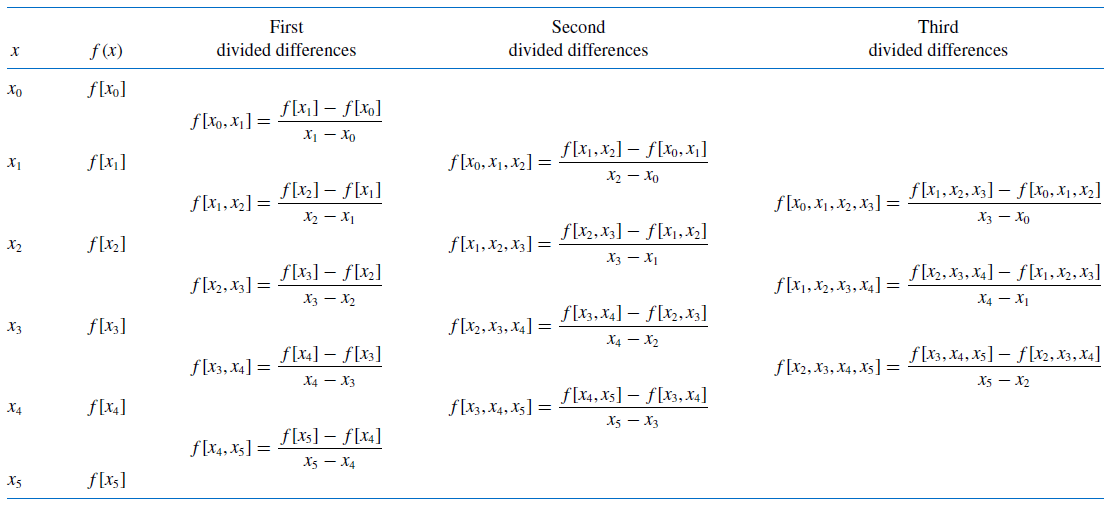
\includegraphics[width=0.99\linewidth]{img06/w06-DividedDifferenceTableExtended} \end{center}

\begin{Shaded}
\begin{Highlighting}[]
\NormalTok{NewtonInterp }\OtherTok{=} \ControlFlowTok{function}\NormalTok{(xvec, }
                        \AttributeTok{yvec =} \ConstantTok{NULL}\NormalTok{, }
                        \AttributeTok{fn =} \ConstantTok{NULL}\NormalTok{,}
\NormalTok{                        pred.x}
\NormalTok{                        )\{}
 \ControlFlowTok{if}\NormalTok{(}\FunctionTok{length}\NormalTok{(yvec)}\SpecialCharTok{==}\DecValTok{0}\NormalTok{) yvec }\OtherTok{=} \FunctionTok{fn}\NormalTok{(xvec)}
\NormalTok{ n}\OtherTok{=}\FunctionTok{length}\NormalTok{(xvec)}
\NormalTok{ DivDiff }\OtherTok{=} \FunctionTok{rep}\NormalTok{(}\DecValTok{0}\NormalTok{,n)         }\CommentTok{\# zero vector to store divided differences}
\NormalTok{ NewtonBasis }\OtherTok{=} \FunctionTok{rep}\NormalTok{(}\DecValTok{0}\NormalTok{,}\DecValTok{1}\NormalTok{)     }\CommentTok{\# zero vector to store Newton form basis polynomial }
\NormalTok{ DivDiff[}\DecValTok{1}\NormalTok{]}\OtherTok{=}\NormalTok{yvec[}\DecValTok{1}\NormalTok{]         }\CommentTok{\# 1st order divided difference loaded to the first}
\NormalTok{ NewtonBasis[}\DecValTok{1}\NormalTok{]}\OtherTok{=}\DecValTok{1}           \CommentTok{\# zero{-}degree basis polynomial}
\NormalTok{ old.NewtonBasis }\OtherTok{=} \DecValTok{1}        \CommentTok{\# initialize Newton basis polynomial for updating newer basis}
 \DocumentationTok{\#\#}
 \ControlFlowTok{for}\NormalTok{ (i }\ControlFlowTok{in} \DecValTok{2}\SpecialCharTok{:}\NormalTok{n)\{}
\NormalTok{    NewtonBasis[i] }\OtherTok{=}\NormalTok{ old.NewtonBasis}\SpecialCharTok{*}\NormalTok{(pred.x}\SpecialCharTok{{-}}\NormalTok{xvec[i}\DecValTok{{-}1}\NormalTok{])  }\CommentTok{\# updating Basis polynomial   }
\NormalTok{    dfx }\OtherTok{=}\NormalTok{ xvec[}\SpecialCharTok{{-}}\NormalTok{(}\DecValTok{1}\SpecialCharTok{:}\NormalTok{(i}\DecValTok{{-}1}\NormalTok{))] }\SpecialCharTok{{-}}\NormalTok{ xvec[}\SpecialCharTok{{-}}\NormalTok{((n}\SpecialCharTok{{-}}\NormalTok{(i}\DecValTok{{-}2}\NormalTok{))}\SpecialCharTok{:}\NormalTok{n)]         }\CommentTok{\# denominator in the divided difference}
\NormalTok{    dy }\OtherTok{=} \FunctionTok{diff}\NormalTok{(yvec)              }\CommentTok{\# difference of lower order divided difference for the numerator}
    \DocumentationTok{\#\#        }
\NormalTok{    DivForm }\OtherTok{=}\NormalTok{ dy}\SpecialCharTok{/}\NormalTok{dfx                   }\CommentTok{\# new vector of divided differences}
\NormalTok{    DivDiff[i]}\OtherTok{=}\NormalTok{DivForm[}\DecValTok{1}\NormalTok{]              }\CommentTok{\# pick the top one store in the vector of DivDiff}
\NormalTok{    yvec }\OtherTok{=}\NormalTok{ DivForm                     }\CommentTok{\# updating for operation in the next row}
\NormalTok{    old.NewtonBasis }\OtherTok{=}\NormalTok{ NewtonBasis[i]   }\CommentTok{\# updating Newton basis polynomial}
\NormalTok{   \}}
\NormalTok{ Nx}\OtherTok{=}\FunctionTok{sum}\NormalTok{(DivDiff}\SpecialCharTok{*}\NormalTok{NewtonBasis)           }\CommentTok{\# predicted y value of the given pred.x}
 \FunctionTok{list}\NormalTok{(}\AttributeTok{Pred.y =}\NormalTok{ Nx, }\AttributeTok{DividedDifference =}\NormalTok{ DivDiff, }\AttributeTok{NewtonBasis =}\NormalTok{ NewtonBasis)}
\NormalTok{\}}
\end{Highlighting}
\end{Shaded}

\textbf{Example 3}: Reproduce the result in the above illustrative table.

\begin{Shaded}
\begin{Highlighting}[]
\NormalTok{vec.x }\OtherTok{=} \FunctionTok{c}\NormalTok{(}\DecValTok{3}\NormalTok{,}\DecValTok{1}\NormalTok{,}\DecValTok{5}\NormalTok{,}\DecValTok{6}\NormalTok{)          }
\NormalTok{vec.y }\OtherTok{=} \FunctionTok{c}\NormalTok{(}\DecValTok{1}\NormalTok{,}\SpecialCharTok{{-}}\DecValTok{3}\NormalTok{,}\DecValTok{2}\NormalTok{,}\DecValTok{4}\NormalTok{)}
\NormalTok{example1 }\OtherTok{=} \FunctionTok{NewtonInterp}\NormalTok{(}\AttributeTok{yvec =}\NormalTok{ vec.y, }\AttributeTok{xvec =}\NormalTok{ vec.x, }\AttributeTok{pred.x =} \DecValTok{5}\NormalTok{)}
\NormalTok{example1}
\end{Highlighting}
\end{Shaded}

\begin{verbatim}
## $Pred.y
## [1] 2
## 
## $DividedDifference
## [1]  1.000  2.000 -0.375  0.175
## 
## $NewtonBasis
## [1] 1 2 8 0
\end{verbatim}

\begin{Shaded}
\begin{Highlighting}[]
\FunctionTok{sum}\NormalTok{(example1}\SpecialCharTok{$}\NormalTok{DividedDifferenc}\SpecialCharTok{*}\NormalTok{ example1}\SpecialCharTok{$}\NormalTok{NewtonBasis)}
\end{Highlighting}
\end{Shaded}

\begin{verbatim}
## [1] 2
\end{verbatim}

\textbf{Example 5}: Reproduce \emph{Example 1} of Burden and Faires' textbook, 9th edition, page 127) Complete the divided difference table for the following data.

\begin{longtable}[]{@{}
  >{\raggedright\arraybackslash}p{(\columnwidth - 2\tabcolsep) * \real{0.0556}}
  >{\centering\arraybackslash}p{(\columnwidth - 2\tabcolsep) * \real{0.1389}}@{}}
\toprule\noalign{}
\begin{minipage}[b]{\linewidth}\raggedright
x
\end{minipage} & \begin{minipage}[b]{\linewidth}\centering
y
\end{minipage} \\
\midrule\noalign{}
\endhead
\bottomrule\noalign{}
\endlastfoot
1.0
1.3
1.6
1.9
2.2 & 0.7651977
0.6200860
0.4554022
0.2818186
0.1103623 \\
\end{longtable}

\begin{Shaded}
\begin{Highlighting}[]
\NormalTok{vec.x }\OtherTok{=} \FunctionTok{c}\NormalTok{(}\DecValTok{1}\NormalTok{, }\FloatTok{1.3}\NormalTok{, }\FloatTok{1.6}\NormalTok{, }\FloatTok{1.9}\NormalTok{, }\FloatTok{2.2}\NormalTok{)          }
\NormalTok{vec.y }\OtherTok{=} \FunctionTok{c}\NormalTok{(}\FloatTok{0.7651977}\NormalTok{, }\FloatTok{0.6200860}\NormalTok{, }\FloatTok{0.4554022}\NormalTok{, }\FloatTok{0.2818186}\NormalTok{, }\FloatTok{0.1103623}\NormalTok{)}
\NormalTok{example2 }\OtherTok{=} \FunctionTok{NewtonInterp}\NormalTok{(}\AttributeTok{yvec =}\NormalTok{ vec.y, }\AttributeTok{xvec =}\NormalTok{ vec.x, }\AttributeTok{pred.x =} \DecValTok{1}\NormalTok{)}
\NormalTok{example2}
\end{Highlighting}
\end{Shaded}

\begin{verbatim}
## $Pred.y
## [1] 0.7651977
## 
## $DividedDifference
## [1]  0.765197700 -0.483705667 -0.108733889  0.065878395  0.001825103
## 
## $NewtonBasis
## [1] 1 0 0 0 0
\end{verbatim}

\begin{Shaded}
\begin{Highlighting}[]
\FunctionTok{sum}\NormalTok{(example2}\SpecialCharTok{$}\NormalTok{DividedDifferenc}\SpecialCharTok{*}\NormalTok{ example2}\SpecialCharTok{$}\NormalTok{NewtonBasis)}
\end{Highlighting}
\end{Shaded}

\begin{verbatim}
## [1] 0.7651977
\end{verbatim}

\hypertarget{vectorizing-newtoninterp}{%
\subsection{\texorpdfstring{Vectorizing \textbf{NewtonInterp()}}{Vectorizing NewtonInterp()}}\label{vectorizing-newtoninterp}}

Next, we vectorize the above R function for Newton interpolation polynomial so that it can take a vector input. We will also compare this new function with the two R functions created in the lecture note.

\begin{Shaded}
\begin{Highlighting}[]
\NormalTok{Vectorizing.Newton }\OtherTok{=} \ControlFlowTok{function}\NormalTok{(xvec, }
                                \AttributeTok{yvec =} \ConstantTok{NULL}\NormalTok{, }
                                \AttributeTok{fn =} \ConstantTok{NULL}\NormalTok{,}
\NormalTok{                                pred.x     }\CommentTok{\# numerical vector or scalar input}
\NormalTok{                        )\{}
 \ControlFlowTok{if}\NormalTok{(}\FunctionTok{length}\NormalTok{(yvec) }\SpecialCharTok{==} \DecValTok{0}\NormalTok{) yvec }\OtherTok{=} \FunctionTok{fn}\NormalTok{(xvec)}
\NormalTok{ n }\OtherTok{=} \FunctionTok{length}\NormalTok{(xvec)  }
\NormalTok{ m }\OtherTok{=} \FunctionTok{length}\NormalTok{(pred.x)            }\CommentTok{\# dimension of the input vector for prediction}
\NormalTok{ NewtonPolynomial }\OtherTok{=} \FunctionTok{rep}\NormalTok{(}\DecValTok{0}\NormalTok{, m)  }\CommentTok{\# predicted value of the Newton interpolation polynomial}
 \ControlFlowTok{for}\NormalTok{ (k }\ControlFlowTok{in} \DecValTok{1}\SpecialCharTok{:}\NormalTok{m)\{}
\NormalTok{    yvec0 }\OtherTok{=}\NormalTok{ yvec     }\CommentTok{\# }\AlertTok{CAUTION}\CommentTok{: Must be REINSTATED! diff(yvec) will change its original values!! }
\NormalTok{    DivDiff }\OtherTok{=} \FunctionTok{rep}\NormalTok{(}\DecValTok{0}\NormalTok{,n)         }\CommentTok{\# zero vector to store divided differences}
\NormalTok{    NewtonBasis }\OtherTok{=} \FunctionTok{rep}\NormalTok{(}\DecValTok{0}\NormalTok{,}\DecValTok{1}\NormalTok{)     }\CommentTok{\# zero vector to store Newton form basis polynomial }
\NormalTok{    DivDiff[}\DecValTok{1}\NormalTok{] }\OtherTok{=}\NormalTok{ yvec[}\DecValTok{1}\NormalTok{]       }\CommentTok{\# 1st order divided difference loaded to the first}
\NormalTok{    NewtonBasis[}\DecValTok{1}\NormalTok{] }\OtherTok{=} \DecValTok{1}         \CommentTok{\# zero{-}degree basis polynomial}
\NormalTok{    old.NewtonBasis }\OtherTok{=} \DecValTok{1}        \CommentTok{\# initialize Newton basis polynomial for updating the newer basis}
    \DocumentationTok{\#\#}
    \ControlFlowTok{for}\NormalTok{ (i }\ControlFlowTok{in} \DecValTok{2}\SpecialCharTok{:}\NormalTok{n)\{}
\NormalTok{       NewtonBasis[i] }\OtherTok{=}\NormalTok{ old.NewtonBasis}\SpecialCharTok{*}\NormalTok{(pred.x[k]}\SpecialCharTok{{-}}\NormalTok{xvec[i}\DecValTok{{-}1}\NormalTok{])  }\CommentTok{\# updating basis polynomial   }
\NormalTok{       dfx }\OtherTok{=}\NormalTok{ xvec[}\SpecialCharTok{{-}}\NormalTok{(}\DecValTok{1}\SpecialCharTok{:}\NormalTok{(i}\DecValTok{{-}1}\NormalTok{))] }\SpecialCharTok{{-}}\NormalTok{ xvec[}\SpecialCharTok{{-}}\NormalTok{((n}\SpecialCharTok{{-}}\NormalTok{(i}\DecValTok{{-}2}\NormalTok{))}\SpecialCharTok{:}\NormalTok{n)]     }\CommentTok{\# denominator in the divided difference}
\NormalTok{       dy }\OtherTok{=} \FunctionTok{diff}\NormalTok{(yvec0)         }\CommentTok{\# difference of lower order divided difference for the numerator}
\NormalTok{       DivForm }\OtherTok{=}\NormalTok{ dy}\SpecialCharTok{/}\NormalTok{dfx         }\CommentTok{\# new vector of divided differences}
       \CommentTok{\#cat("\textbackslash{}n\textbackslash{}n Inner loop:",i,". dfx =",dfx, ". dy =", dy, ". ")}
\NormalTok{       DivDiff[i] }\OtherTok{=}\NormalTok{ DivForm[}\DecValTok{1}\NormalTok{]  }\CommentTok{\# pick 1st component to store in vector DivDiff}
\NormalTok{       yvec0 }\OtherTok{=}\NormalTok{ DivForm          }\CommentTok{\# updating for operation in the next row}
\NormalTok{       old.NewtonBasis }\OtherTok{=}\NormalTok{ NewtonBasis[i]}
\NormalTok{      \}}
\NormalTok{      NewtonPolynomial[k] }\OtherTok{=} \FunctionTok{sum}\NormalTok{(DivDiff}\SpecialCharTok{*}\NormalTok{NewtonBasis)}
      \CommentTok{\#cat("\textbackslash{}n\textbackslash{}n",k,"{-}th Pred.y:",NewtonPolynomial,", Diff:", DivDiff, ", Basis:", NewtonBasis,".")}
\NormalTok{     \}}
\NormalTok{ NewtonPolynomial}
\NormalTok{\}}
\end{Highlighting}
\end{Shaded}

\begin{Shaded}
\begin{Highlighting}[]
\NormalTok{vec.x }\OtherTok{=} \FunctionTok{c}\NormalTok{(}\DecValTok{1}\NormalTok{, }\FloatTok{1.3}\NormalTok{, }\FloatTok{1.6}\NormalTok{, }\FloatTok{1.9}\NormalTok{, }\FloatTok{2.2}\NormalTok{)          }
\NormalTok{vec.y }\OtherTok{=} \FunctionTok{c}\NormalTok{(}\FloatTok{0.7651977}\NormalTok{, }\FloatTok{0.6200860}\NormalTok{, }\FloatTok{0.4554022}\NormalTok{, }\FloatTok{0.2818186}\NormalTok{, }\FloatTok{0.1103623}\NormalTok{)}
\FunctionTok{Vectorizing.Newton}\NormalTok{(}\AttributeTok{yvec =}\NormalTok{ vec.y, }\AttributeTok{xvec =}\NormalTok{ vec.x, }\AttributeTok{pred.x =} \FunctionTok{c}\NormalTok{(}\DecValTok{1}\NormalTok{, }\DecValTok{2}\NormalTok{))}
\end{Highlighting}
\end{Shaded}

\begin{verbatim}
## [1] 0.7651977 0.2238754
\end{verbatim}

\hypertarget{code-efficiency-with-implivit-loops}{%
\subsection{Code Efficiency with Implivit Loops}\label{code-efficiency-with-implivit-loops}}

For comparison, we copy the two functions in the lecture note.

\begin{Shaded}
\begin{Highlighting}[]
\NormalTok{Divided.Dif }\OtherTok{=} \ControlFlowTok{function}\NormalTok{(}
\NormalTok{        vec.x,          }\CommentTok{\# input nodes:}
        \AttributeTok{vec.y =} \ConstantTok{NULL}\NormalTok{,   }\CommentTok{\# one of vec.y and fn must be given}
        \AttributeTok{fn =} \ConstantTok{NULL}\NormalTok{,}
\NormalTok{        pred.x          }\CommentTok{\# scalar x for predicting pn(pred.x)}
\NormalTok{         )\{}
\NormalTok{   n }\OtherTok{=} \FunctionTok{length}\NormalTok{(vec.x)}
   \ControlFlowTok{if}\NormalTok{ (}\FunctionTok{length}\NormalTok{(vec.y) }\SpecialCharTok{==} \DecValTok{0}\NormalTok{) vec.y }\OtherTok{=} \FunctionTok{fn}\NormalTok{(vec.x) }\CommentTok{\#}
\NormalTok{   node.x }\OtherTok{=}\NormalTok{ vec.x}
\NormalTok{   A }\OtherTok{=} \FunctionTok{matrix}\NormalTok{(}\FunctionTok{c}\NormalTok{(}\FunctionTok{rep}\NormalTok{(}\DecValTok{0}\NormalTok{,n}\SpecialCharTok{\^{}}\DecValTok{2}\NormalTok{)), }\AttributeTok{nrow =}\NormalTok{ n, }\AttributeTok{ncol =}\NormalTok{ n, }\AttributeTok{byrow =} \ConstantTok{TRUE}\NormalTok{)}
\NormalTok{   A[}\DecValTok{1}\NormalTok{,] }\OtherTok{=}\NormalTok{ vec.y     }\CommentTok{\# fill the first row with vec.y}
   \CommentTok{\#}
   \ControlFlowTok{for}\NormalTok{(i }\ControlFlowTok{in} \DecValTok{2}\SpecialCharTok{:}\NormalTok{(n))\{}
     \ControlFlowTok{for}\NormalTok{(j }\ControlFlowTok{in} \DecValTok{1}\SpecialCharTok{:}\NormalTok{(n}\SpecialCharTok{{-}}\NormalTok{i}\SpecialCharTok{+}\DecValTok{1}\NormalTok{))\{}
\NormalTok{      denominator }\OtherTok{=}\NormalTok{ vec.x[j] }\SpecialCharTok{{-}}\NormalTok{ vec.x[j}\SpecialCharTok{+}\DecValTok{1}\SpecialCharTok{+}\NormalTok{(i}\DecValTok{{-}2}\NormalTok{)]}
\NormalTok{      numerator }\OtherTok{=}\NormalTok{ A[i}\DecValTok{{-}1}\NormalTok{,j]}\SpecialCharTok{{-}}\NormalTok{ A[i}\DecValTok{{-}1}\NormalTok{,j}\SpecialCharTok{+}\DecValTok{1}\NormalTok{]}
\NormalTok{      A[i,j] }\OtherTok{=}\NormalTok{ numerator}\SpecialCharTok{/}\NormalTok{denominator}
\NormalTok{      \}}
\NormalTok{    \}}
\NormalTok{  A}
\NormalTok{ \}}
\end{Highlighting}
\end{Shaded}

\begin{Shaded}
\begin{Highlighting}[]
\DocumentationTok{\#\#\#\#\#\#\#\#\#\#\#\#\#\#\#\#\#\#\#\#\#\#\#\#\#\#\#\#\#\#\#\#\#\#\#\#\#\#\#\#\#\#\#\#\#\#\#\#\#\#\#\#\#\#\#\#\#\#\#\#\#\#\#\#\#\#\#\#\#\#\#\#\#\#\#\#\#\#\#\#\#\#}
\DocumentationTok{\#\#  Newton Interpolated Polynomial Approximation: vector{-}enabled input}
\DocumentationTok{\#\#\#\#\#\#\#\#\#\#\#\#\#\#\#\#\#\#\#\#\#\#\#\#\#\#\#\#\#\#\#\#\#\#\#\#\#\#\#\#\#\#\#\#\#\#\#\#\#\#\#\#\#\#\#\#\#\#\#\#\#\#\#\#\#\#\#\#\#\#\#\#\#\#\#\#\#\#\#\#\#\#}

\NormalTok{Looping.Newton }\OtherTok{=} \ControlFlowTok{function}\NormalTok{( vec.x,            }\CommentTok{\# input interpolation nodes}
                                \AttributeTok{vec.y =} \ConstantTok{NULL}\NormalTok{,    }
                                \AttributeTok{fn =} \ConstantTok{NULL}\NormalTok{,        }\CommentTok{\# either vec.y or fn must be provided}
\NormalTok{                                pred.x            }\CommentTok{\# VECTOR INPUT!!!}
\NormalTok{                              )\{}
   \ControlFlowTok{if}\NormalTok{(}\FunctionTok{length}\NormalTok{(vec.y) }\SpecialCharTok{==}\DecValTok{0}\NormalTok{) vec.y }\OtherTok{=} \FunctionTok{fn}\NormalTok{(vec.x)}
\NormalTok{   DivDif }\OtherTok{=} \FunctionTok{Divided.Dif}\NormalTok{(vec.x, vec.y)[,}\DecValTok{1}\NormalTok{]       }\CommentTok{\# the values in the first column of the div dif matrix}
\NormalTok{   n }\OtherTok{=} \FunctionTok{length}\NormalTok{(vec.x)}
   \DocumentationTok{\#\#\#\#\#\#\#\#\#\#\#\#}
\NormalTok{   m }\OtherTok{=} \FunctionTok{length}\NormalTok{(pred.x)}
\NormalTok{   NV }\OtherTok{=} \FunctionTok{rep}\NormalTok{(}\DecValTok{0}\NormalTok{, m)                 }\CommentTok{\# values of Nn(pred.x)}
   \ControlFlowTok{for}\NormalTok{(k }\ControlFlowTok{in} \DecValTok{1}\SpecialCharTok{:}\NormalTok{m) \{}
   \DocumentationTok{\#\#\#\#\#\#\#\#\#\#\#\#\#\#\#\#}
\NormalTok{   Nn }\OtherTok{=}\NormalTok{ vec.y[}\DecValTok{1}\NormalTok{]                  }\CommentTok{\# f[xo]}
   \ControlFlowTok{for}\NormalTok{ (i }\ControlFlowTok{in} \DecValTok{1}\SpecialCharTok{:}\NormalTok{(n}\DecValTok{{-}1}\NormalTok{))\{            }\CommentTok{\# Must be n {-} 1 according to the last term in the polynomial}
\NormalTok{     cumProd }\OtherTok{=} \DecValTok{1}                  \CommentTok{\# initial value to calculate the cumulative product}
     \ControlFlowTok{for}\NormalTok{(j }\ControlFlowTok{in} \DecValTok{1}\SpecialCharTok{:}\NormalTok{i)\{               }\CommentTok{\# forward difference formula}
\NormalTok{       cumProd }\OtherTok{=}\NormalTok{ cumProd}\SpecialCharTok{*}\NormalTok{(pred.x[k]}\SpecialCharTok{{-}}\NormalTok{vec.x[j])   }\CommentTok{\# updating the cumulative product in the inner loop}
\NormalTok{     \}}
\NormalTok{      Nn }\OtherTok{=}\NormalTok{ Nn }\SpecialCharTok{+}\NormalTok{ DivDif[i}\SpecialCharTok{+}\DecValTok{1}\NormalTok{]}\SpecialCharTok{*}\NormalTok{cumProd    }\CommentTok{\# adding high order terms alliteratively to the Nn(x) }
\NormalTok{    \}}
\NormalTok{    NV[k] }\OtherTok{=}\NormalTok{ Nn                                  }\CommentTok{\# return the value the Newton polynomial}
\NormalTok{   \}}
\NormalTok{ NV  }
\NormalTok{\}}
\end{Highlighting}
\end{Shaded}

The following code shows the computational time the above two functions take in the approximation.

\begin{Shaded}
\begin{Highlighting}[]
\NormalTok{start }\OtherTok{\textless{}{-}} \FunctionTok{Sys.time}\NormalTok{()}
\NormalTok{pred.x }\OtherTok{=} \FunctionTok{c}\NormalTok{(}\FloatTok{1.6}\NormalTok{, }\FloatTok{1.1}\NormalTok{, }\FloatTok{2.0}\NormalTok{)   }\CommentTok{\# pred.x is the argument is a local variable!}
\NormalTok{pred.NIP0 }\OtherTok{=} \FunctionTok{Vectorizing.Newton}\NormalTok{(}\AttributeTok{xvec =} \FunctionTok{c}\NormalTok{(}\DecValTok{1}\NormalTok{, }\FloatTok{1.3}\NormalTok{, }\FloatTok{1.6}\NormalTok{, }\FloatTok{1.9}\NormalTok{, }\FloatTok{2.2}\NormalTok{),           }
                    \AttributeTok{yvec =} \FunctionTok{c}\NormalTok{(}\FloatTok{0.7651977}\NormalTok{, }\FloatTok{0.6200860}\NormalTok{, }\FloatTok{0.4554022}\NormalTok{, }\FloatTok{0.2818186}\NormalTok{, }\FloatTok{0.1103623}\NormalTok{), }
                    \AttributeTok{pred.x =} \FunctionTok{c}\NormalTok{(}\FloatTok{1.6}\NormalTok{, }\FloatTok{1.1}\NormalTok{, }\FloatTok{2.0}\NormalTok{))}
\FunctionTok{pander}\NormalTok{(}\FunctionTok{cbind}\NormalTok{(}\AttributeTok{pred.x =}\NormalTok{ pred.x, }\AttributeTok{pred.NIP=}\NormalTok{pred.NIP0))}
\end{Highlighting}
\end{Shaded}

\begin{longtable}[]{@{}
  >{\centering\arraybackslash}p{(\columnwidth - 2\tabcolsep) * \real{0.1250}}
  >{\centering\arraybackslash}p{(\columnwidth - 2\tabcolsep) * \real{0.1528}}@{}}
\toprule\noalign{}
\begin{minipage}[b]{\linewidth}\centering
pred.x
\end{minipage} & \begin{minipage}[b]{\linewidth}\centering
pred.NIP
\end{minipage} \\
\midrule\noalign{}
\endhead
\bottomrule\noalign{}
\endlastfoot
1.6 & 0.4554 \\
1.1 & 0.7196 \\
2 & 0.2239 \\
\end{longtable}

\begin{Shaded}
\begin{Highlighting}[]
\FunctionTok{print}\NormalTok{( }\FunctionTok{Sys.time}\NormalTok{() }\SpecialCharTok{{-}}\NormalTok{ start )}
\end{Highlighting}
\end{Shaded}

\begin{verbatim}
## Time difference of 0.01160407 secs
\end{verbatim}

\begin{Shaded}
\begin{Highlighting}[]
\NormalTok{start }\OtherTok{\textless{}{-}} \FunctionTok{Sys.time}\NormalTok{()}
\NormalTok{pred.x }\OtherTok{=} \FunctionTok{c}\NormalTok{(}\FloatTok{1.6}\NormalTok{, }\FloatTok{1.1}\NormalTok{, }\FloatTok{2.0}\NormalTok{)   }\CommentTok{\# pred.x is the argument is a local variable!}
\NormalTok{pred.NIP }\OtherTok{=} \FunctionTok{Looping.Newton}\NormalTok{(}\AttributeTok{vec.x =} \FunctionTok{c}\NormalTok{(}\DecValTok{1}\NormalTok{, }\FloatTok{1.3}\NormalTok{, }\FloatTok{1.6}\NormalTok{, }\FloatTok{1.9}\NormalTok{, }\FloatTok{2.2}\NormalTok{),           }
                    \AttributeTok{vec.y =} \FunctionTok{c}\NormalTok{(}\FloatTok{0.7651977}\NormalTok{, }\FloatTok{0.6200860}\NormalTok{, }\FloatTok{0.4554022}\NormalTok{, }\FloatTok{0.2818186}\NormalTok{, }\FloatTok{0.1103623}\NormalTok{), }
                    \AttributeTok{pred.x =} \FunctionTok{c}\NormalTok{(}\FloatTok{1.6}\NormalTok{, }\FloatTok{1.1}\NormalTok{, }\FloatTok{2.0}\NormalTok{))}
\FunctionTok{pander}\NormalTok{(}\FunctionTok{cbind}\NormalTok{(}\AttributeTok{pred.x =}\NormalTok{ pred.x, }\AttributeTok{pred.NIP=}\NormalTok{pred.NIP))}
\end{Highlighting}
\end{Shaded}

\begin{longtable}[]{@{}
  >{\centering\arraybackslash}p{(\columnwidth - 2\tabcolsep) * \real{0.1250}}
  >{\centering\arraybackslash}p{(\columnwidth - 2\tabcolsep) * \real{0.1528}}@{}}
\toprule\noalign{}
\begin{minipage}[b]{\linewidth}\centering
pred.x
\end{minipage} & \begin{minipage}[b]{\linewidth}\centering
pred.NIP
\end{minipage} \\
\midrule\noalign{}
\endhead
\bottomrule\noalign{}
\endlastfoot
1.6 & 0.4554 \\
1.1 & 0.7196 \\
2 & 0.2239 \\
\end{longtable}

\begin{Shaded}
\begin{Highlighting}[]
\FunctionTok{print}\NormalTok{( }\FunctionTok{Sys.time}\NormalTok{() }\SpecialCharTok{{-}}\NormalTok{ start )}
\end{Highlighting}
\end{Shaded}

\begin{verbatim}
## Time difference of 0.02802587 secs
\end{verbatim}

\hypertarget{gauss-elimination-method}{%
\chapter{Gauss Elimination Method}\label{gauss-elimination-method}}

We discuss numerical solutions to the linear system of equations. Consider the following general linear system of equations

\begin{center}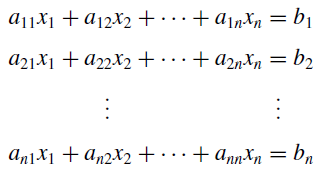
\includegraphics[width=0.35\linewidth]{img07/w07-LinearSysEq} \end{center}

The goal is to find the solution to this system. There are different methods to solve the linear system. One way is to re-express the linear system into a matrix equation and then solve the matrix equation.

\textbf{Example 1} Consider the following linear system of functions

\[
\begin{array}{ccc}
3x_1 - x_2 + 2x_3 & = & 8  \\ 
2x_1 - 2x_2 + 3x_3 & = & 2 \\ 
4x_1 + x_2 - 4x_3 & = & 9 
\end{array}
\]

We can re-write the above system of linear equations into the following matrix form

\begin{center}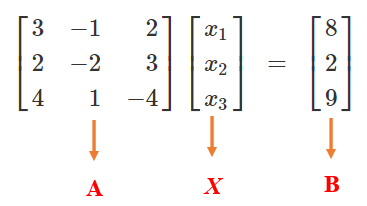
\includegraphics[width=0.45\linewidth]{img07/w07-Example01MatrixForm} \end{center}

We denote

\[
\mathbf{A} = \left[
\begin{array}{ccc}
 3 & -1 &  2 \\ 
 2 & -2 &  3 \\ 
 4 &  1 & -4 
\end{array}
\right]
\]
be the coefficient matrix.

\[
\mathbf{X} = \left[ \begin{array}{c} x_1 \\ x_2 \\ x_3  \end{array} \right]
\]

the vector of unknown, and

\[
\mathbf{B} = \left[ \begin{array}{c} 8 \\ 2 \\ 9  \end{array} \right]
\]

Then, the matrix form of the equation is equivalent to \(\mathbf{A}\mathbf{X} ~=~ \mathbf{B}\). If the inverse of \(\mathbf{A}\), denoted by \(\mathbf{A}^{-1}\), exists, we multiply \(\mathbf{A}^{-1}\) to the left of the matrix equation to get the solution of the linear system in the following

\[
\mathbf{X} = \mathbf{A}^{-1}\mathbf{B}
\]

Finding the inverse of the matrix could be a challenge when the system is large. The R built-in function \texttt{solve()} to calculate the inverse of a matrix (if it exists).
For example, the inverse of \(\mathbf{A}\) can be found using the following code.

\begin{Shaded}
\begin{Highlighting}[]
\NormalTok{A }\OtherTok{=} \FunctionTok{matrix}\NormalTok{(}\FunctionTok{c}\NormalTok{(}\DecValTok{3}\NormalTok{, }\SpecialCharTok{{-}}\DecValTok{1}\NormalTok{, }\DecValTok{2}\NormalTok{, }\DecValTok{2}\NormalTok{, }\SpecialCharTok{{-}}\DecValTok{2}\NormalTok{, }\DecValTok{3}\NormalTok{, }\DecValTok{4}\NormalTok{, }\DecValTok{1}\NormalTok{, }\SpecialCharTok{{-}}\DecValTok{4}\NormalTok{), }\AttributeTok{ncol =} \DecValTok{3}\NormalTok{, }\AttributeTok{byrow =} \ConstantTok{TRUE}\NormalTok{)}
\NormalTok{A.inv }\OtherTok{=} \FunctionTok{solve}\NormalTok{(A)}
\NormalTok{A.inv        }\CommentTok{\# print out the }
\end{Highlighting}
\end{Shaded}

\begin{verbatim}
##           [,1]       [,2]        [,3]
## [1,] 0.3333333 -0.1333333  0.06666667
## [2,] 1.3333333 -1.3333333 -0.33333333
## [3,] 0.6666667 -0.4666667 -0.26666667
\end{verbatim}

\begin{Shaded}
\begin{Highlighting}[]
\CommentTok{\# matrix multiplication}
\NormalTok{A}\SpecialCharTok{\%*\%}\NormalTok{A.inv    }\CommentTok{\# expected to be the identity matrix}
\end{Highlighting}
\end{Shaded}

\begin{verbatim}
##      [,1]          [,2]          [,3]
## [1,]    1 -2.220446e-16 -2.220446e-16
## [2,]    0  1.000000e+00 -1.110223e-16
## [3,]    0  0.000000e+00  1.000000e+00
\end{verbatim}

Two ways to find the solution to the system

\begin{Shaded}
\begin{Highlighting}[]
\NormalTok{B }\OtherTok{=} \FunctionTok{c}\NormalTok{(}\DecValTok{8}\NormalTok{,}\DecValTok{2}\NormalTok{,}\DecValTok{9}\NormalTok{)}
\NormalTok{X}\FloatTok{.1} \OtherTok{=} \FunctionTok{solve}\NormalTok{(A)}\SpecialCharTok{\%*\%}\NormalTok{B  }\CommentTok{\# returns a matrix form solution}
\NormalTok{X}\FloatTok{.1}    
\end{Highlighting}
\end{Shaded}

\begin{verbatim}
##      [,1]
## [1,]    3
## [2,]    5
## [3,]    2
\end{verbatim}

\begin{Shaded}
\begin{Highlighting}[]
\NormalTok{X}\FloatTok{.2} \OtherTok{=} \FunctionTok{solve}\NormalTok{(A,B)   }\CommentTok{\# returns a vector form solution}
\NormalTok{X}\FloatTok{.2}
\end{Highlighting}
\end{Shaded}

\begin{verbatim}
## [1] 3 5 2
\end{verbatim}

\hypertarget{naive-gaussian-elimination-methods}{%
\section{Naive Gaussian Elimination Methods}\label{naive-gaussian-elimination-methods}}

Linear algebra texts discuss elimination methods to find the solution. The method has two processes: elimination and backward substitution. We use the equation in the above \textbf{Example 1} to review the elimination method.

Recall the linear system

\[
\begin{array}{ccc}
3x_1 - x_2 + 2x_3 & = & 8  \\ 
2x_1 - 2x_2 + 3x_3 & = & 2 \\ 
4x_1 + x_2 - 4x_3 & = & 9 
\end{array}
\]

We define the following augmented matrix.

\[
\mathbf{A} = \left[
\begin{array}{ccccc}
 3 & -1 & 2 & \vdots & 8\\ 
 2 & -2 & 3 & \vdots & 2\\ 
 4 & 1 & -4 & \vdots & 9\\ 
\end{array}
\right]
\]

\textbf{Solution} We show the detailed steps of forward elimination and backward substitution.

\textbf{Forward Elimination}

We use \(R_1\), \(R_2\), and \(R_3\) to denote the three rows of the above-augmented matrix and then find the solution in the following \(r = 3 - 1\) steps:

\textbf{Step 1} The equation in the first row is called \textbf{pivot equation} and \(a_{11} = 3\) is called \textbf{pivot element}. We first do the following row operations so that the elements in the first column of the resulting \textbf{new augmented} matrix are all zeros except for the one in the \emph{pivot} element.

\emph{1.1}. Multiply \(-a_{21}/a_{11}\) to \(R_1\) and add it to \(R_2\) to update \(R_2\). \textbf{Row 2}: \(i = 2\)

\[
R_2 \leftarrow R_2 -(a_{21}/a_{11})\times R_1  = (a_{21}, a_{22}, a_{23}, b_2) - \frac{a_{21}}{a_{11}}(a_{11}, a_{12}, a_{13}, b_1)
\]

\[
= (a_{21} - \frac{a_{21}}{a_{11}}\times a_{11}, a_{22} - \frac{a_{21}}{a_{11}}\times a_{12}, a_{23}-\frac{a_{21}}{a_{11}}\times a_{11}, b_2-\frac{a_{21}}{a_{11}}\times a_{11})
\]

\[
=(2,-2, 3, 2) - \frac{2}{3}(3,-1,2,8)  = (0, -4/3, 5/3, -10/3)
\]

\textbf{\color{red}The above step can be computed using the implicit loop through vector operation in any vectorized programming language}

\emph{1.2} Multiply \(-4/3\) to \(R_1\) and add it to \(R_3\) to update \(R_3.\) \textbf{Row 3}: \(i = 3\)

\[
R_3 \leftarrow R_3 - (a_{31}/a_{11}) \times R1  = (a_{31}, a_{32}, a_{33}, b_3) - \frac{a_{31}}{a_{11}}(a_{11}, a_{12}, a_{13}, b_1) 
\]

\[
=(4,1,-4,9) - \frac{4}{3}(3, -1, 2, 8) = \left(0, \frac{7}{3}, -\frac{20}{3}, -\frac{5}{3} \right)
\]

After this step, we have the updated augmented matrix for the next step elimination.

\[
\left[
\begin{array}{ccccc}
 3 & -1 & 2 & \vdots & 8\\ 
 0 & -4/3 & 5/3 & \vdots & -10/3\\ 
 0 & 7/3 & -20/3 & \vdots & -5/3\\ 
\end{array}
\right]
\]

\textbf{Step 2}: The equation in the first row is called \emph{pivot equation} and \(a_{22} = -4/3\) (\textbf{CAUTION}: \emph{using the above updated augmented matrix!})is called pivot element. We next do row operation: \(R_3 - \frac{a_{32}}{a_{22}}\times R_2\) so that the resulting new augmented matrix. \textbf{Row 3}: \(r = 3\).

\[
R_3 \leftarrow R_3 - \frac{a_{32}}{a_{22}}\times R_2 = (a_{31}, a_{32}, a_{33}, b_3) - \frac{a_{32}}{a_{22}}(a_{21}, a_{22}, a_{23}, b_2)
\]

\[
= \left( 0, \frac{7}{3}, -\frac{20}{3}, -\frac{5}{3}\right) - \frac{7/3}{-4/3}\left(0, -\frac{4}{3}, \frac{5}{3}, -\frac{-10}{3} \right)  = \left(0, ~~0, ~~-\frac{15}{4}, -\frac{15}{2} \right)
\]

With the above row operation, we have the following updated augmented matrix that has a triangular coefficient matrix.

\[
\left[
\begin{array}{ccccc}
 3 & -1 & 2 & \vdots & 8\\ 
 0 & -4/3 & 5/3 & \vdots & -10/3\\ 
 0 & 0 & -15/4 & \vdots & -15/2\\ 
\end{array}
\right].
\]

If we re-write the above-augmented matrix into the linear system of equations, we have

\[
\left\{
\begin{array}{ccccc} 
 3x_1 & - x_2 & 2x_3 & = & 8\\ 
   & -\frac{4}{3}x_2 & \frac{5}{3}x_3 & = & -\frac{10}{3}\\ 
   &  & -\frac{15}{4}x_3 & = & -\frac{15}{2}\\ 
\end{array}
\right.
\]

\textbf{Backward Substitution}

Next, we do backward substitution to find the solution to the system. The general backward substitution is given by

\[
x_i =\frac{1}{a_{ii}}\left(b_i-\sum_{j=i+1}^3 a_{ij}x_j \right),
\]

where \(i = 3-1, 3-2\). However \(i = 3\)

\[
x_3 =  \frac{b_3}{a_{33}} = \frac{-15/2}{-15/4} = 2.
\]

We start from \textbf{row 3} of the last augmented matrix:

\textbf{Row \#3}: \(r = 3\):

\[
x_3 = \frac{b_3}{a_{33}} = \frac{-15/2}{-15/4} = 2.
\]
\textbf{Row \#2}: \(r=2\)
\[
x_2 = \frac{1}{a_{22}}\left( b_2 - a_{23}x_3 \right)= -\frac{1}{4/3}\left(-\frac{10}{3} - \frac{5}{3}\times 2\right) = \frac{3}{4}\frac{20}{3} = 5.
\]

\textbf{Row \#1}: \(r = 1\)

\[
x_1 = \frac{1}{a_{11}} \left(b_1 -[a_{12}x_2 + a_{13}x_3]  \right) = \frac{1}{3}\left(8-[-1\times 5 + 2\times 2]\right) = \frac{1}{3}(8-(-1)) = 3. 
\]

Therefore, the solution to the above system linear equation is \((x_1, x_2, x_3) = (3, 5, 2)\).

\textbf{Remark}: We re-arrange the following linear system of linear equations

\[
\left\{
\begin{array}{ccccc} 
 3x_1 & - x_2 & 2x_3 & = & 8\\ 
   & -\frac{4}{3}x_2 & \frac{5}{3}x_3 & = & -\frac{10}{3}\\ 
   &  & -\frac{15}{4}x_3 & = & -\frac{15}{2}\\ 
\end{array}
\right.
\]

to get the following equivalent linear system

\[
\left\{
\begin{array}{ccccc} 
 -\frac{15}{4}x_3 &  &  & = & -\frac{15}{2}\\ 
  \frac{5}{3}x_3& -\frac{4}{3}x_2 &  & = & -\frac{10}{3}\\ 
 2x_3  & -x_2 & + 3x_1 & = & 8\\ 
\end{array}
\right.
\]

That can be re-written in the following matrix form

\[
\left[
\begin{array}{ccc}
 -\frac{15}{4} & 0 &  0 \\ 
 \frac{5}{3} & -\frac{4}{3} &  0 \\ 
 2&  -1 & 3 
\end{array}
\right]
\left[ \begin{array}{c} x_3 \\ x_2 \\ x_1  \end{array} \right]
=
\left[ \begin{array}{c}-\frac{15}{2} \\ -\frac{10}{3} \\ 8  \end{array} \right]
\]

The augmented matrix of the above linear system of equations can be written as

\[
\left[
\begin{array}{ccccc}
 -\frac{15}{4} & 0 &  0 &\vdots & -\frac{15}{2}\\ 
 \frac{5}{3} & -\frac{4}{3} &  0 &\vdots & -\frac{10}{3} \\ 
 2 &  -1 & 3 & \vdots & 8
\end{array}
\right]
\]

We can repeat the Gaussian \textbf{forward elimination} with the above-augmented matrix:

\begin{enumerate}
\def\labelenumi{\arabic{enumi}.}
\tightlist
\item
  pivot element \(a_{11} = -\frac{15}{4}\)
\end{enumerate}

\[
R_2 \leftarrow R_2-\frac{a_{21}}{a_{11}}R_1 = \left(\frac{5}{3}, -\frac{4}{3},0, -\frac{10}{3} \right)-\frac{5/3}{-15/4}\left(-\frac{15}{4}, 0, 0, -\frac{15}{2} \right) =\left(0, -\frac{4}{3}, 0, -\frac{20}{3} \right)
\]

\[
R_3 \leftarrow R_3 - \frac{a_{31}}{a_{11}}R_1 = \left(2,-1,3,8 \right) - \frac{2}{-15/4}\left(-\frac{15}{4}, 0, 0, -\frac{15}{2} \right) = \left(0,-1, 3, 4 \right)
\]

We obtain the following updated augmented matrix

\[
\left[
\begin{array}{ccccc}
 -\frac{15}{4} & 0 &  0 &\vdots & -\frac{15}{2}\\ 
 0 & -\frac{4}{3} &  0 &\vdots & -\frac{20}{3} \\ 
 0 &  -1 & 3 & \vdots & 4
\end{array}
\right]
\]
We need one more row operation on the above-augmented matrix

\[
R_3 \leftarrow R_3 - \frac{a_{32}}{a_{22}}R_2 = \left(0, -1, 3, 4 \right) - \frac{-1}{-4/3}\left(0, -\frac{4}{3}, 0, -\frac{20}{3} \right) = \left(0, 0, 3, 9 \right)
\]

The final augmented matrix has the following form

\[
\left[
\begin{array}{ccccc}
 -\frac{15}{4} & 0 &  0 &\vdots & -\frac{15}{2}\\ 
 0 & -\frac{4}{3} &  0 &\vdots & -\frac{20}{3} \\ 
 0 &  0 & 3 & \vdots & 9
\end{array}
\right].
\]
Its equivalent linear system is given by

\[
\left\{
\begin{array}{ccc} 
 -\frac{15}{4}x_3 & = & -\frac{15}{2}\\ 
  -\frac{4}{3}x_2 &  = & -\frac{20}{3}\\ 
   3x_1 & = & 9\\ 
\end{array}
\right.
\]
Therefore, the solution to the original system of equation is (using vector operation - pair-wise division)

\[
(x_3, x_2, x_1) = \frac{(-15/2, -20/3, 9)}{(-15/4, -4/3, 3)} = (2,5,3)
\]

We will apply the logic used in this example to implement the \textbf{Gaussian Elimination method} (using \emph{backward substitution}).

\hfill\break

\hypertarget{gaussian-elimination-algorithm}{%
\section{Gaussian Elimination Algorithm}\label{gaussian-elimination-algorithm}}

In the elimination step, the first row of the augmented matrix is the basis, and all other elements (cells) in the augmented matrix are updated iteratively using the algorithm using the recursive formula

\[
R_i \leftarrow (a_{i1}, a_{i2}, \cdots, a_{in}, b_i) - \frac{a_{ik}}{a_{kk}}(a_{k1}, a_{k2}, \cdots, a_{kn}, b_k)   
\]

where

\begin{itemize}
\item
  \(k = 1, 2, \cdots, n-1\), the iteration index for selecting the \emph{pivot element}.
\item
  \(i = k+1, k+2, ...n\), the iterator of the row of the augmented matrix.
\end{itemize}

\hfill\break

We focus on Gaussian row elimination. The Gaussian forward elimination and backward substitution (Gauss-Jordan) are optional.

The algorithm of Gaussian is relatively simple compared with the iterative algorithms we learned earlier. We only need to convert the following recursive equation to an algorithm with double loops to accomplish the Gaussian forward elimination.

\textbf{Gaussian Forward Elimination Algorithm}

\begin{verbatim}
INPUT: A    (augmented matrix)

OUTPUT: A0  (row-echelon matrix)

STEP 1: find n = # of row

STEP 2: FOR i = 1 TO n
        STEP 3:  IF A[i,i] == 0 DO: 
                    find j with A[j,i] != 0
                    swap row i and row j
                 ENDIF
         
        STEP 4:  IF A[i,i] != 0 DO:
                    FOR j = i + 1 TO n DO: 
                       A[j,] = A[j,]-(A[j,i]/A[i,i])*A[i,]
                    ENDFOR
                 ENDIF
STEP 5: RETURN A0   
\end{verbatim}

The vector operation was used in \textbf{Step 4} of the pseudo-code. Row-swapping in \textbf{step 3} could also involve vector operation.

Next, we write R code to implement the pseudo-code.

\begin{Shaded}
\begin{Highlighting}[]
\NormalTok{Gauss.Elimination }\OtherTok{=} \ControlFlowTok{function}\NormalTok{(A)\{}
  \CommentTok{\# Input A: augmented matrix. Make sure that he diagonal }
  \CommentTok{\#          elements of the coefficient matrix are non{-}zero! }
\NormalTok{  A0 }\OtherTok{=}\NormalTok{ A        }
\NormalTok{  n }\OtherTok{=} \FunctionTok{dim}\NormalTok{(A0)[}\DecValTok{1}\NormalTok{]                }\CommentTok{\# number of rows}
  \ControlFlowTok{for}\NormalTok{(i }\ControlFlowTok{in} \DecValTok{1}\SpecialCharTok{:}\NormalTok{(n}\DecValTok{{-}1}\NormalTok{))\{            }\CommentTok{\# iterator fo pivot element A0[i,i]}
                                \CommentTok{\# i = 1, 2, ..., n{-}1}
      \CommentTok{\#\textasciitilde{}\textasciitilde{}\textasciitilde{}\textasciitilde{}\textasciitilde{}\textasciitilde{}\textasciitilde{}\textasciitilde{}\textasciitilde{}\textasciitilde{}\textasciitilde{}\textasciitilde{}\textasciitilde{}\textasciitilde{}\textasciitilde{}\textasciitilde{}\textasciitilde{}\textasciitilde{}\textasciitilde{}\textasciitilde{}\textasciitilde{}   Make the function robust  \textasciitilde{}\textasciitilde{}\textasciitilde{}\textasciitilde{}\textasciitilde{}\textasciitilde{}\textasciitilde{}\textasciitilde{}\textasciitilde{}\textasciitilde{}\textasciitilde{}\textasciitilde{}\textasciitilde{}\textasciitilde{}\textasciitilde{}\textasciitilde{}\textasciitilde{}\textasciitilde{}\textasciitilde{}\textasciitilde{}\textasciitilde{}\textasciitilde{}\textasciitilde{}\textasciitilde{}\textasciitilde{}\#}
      \ControlFlowTok{if}\NormalTok{(A0[i,i] }\SpecialCharTok{==} \DecValTok{0}\NormalTok{)\{}
\NormalTok{          non}\FloatTok{.0} \OtherTok{=} \FunctionTok{which}\NormalTok{(A0[,i] }\SpecialCharTok{!=} \DecValTok{0}\NormalTok{)}
              \CommentTok{\#cat("\textbackslash{}n\textbackslash{}n i =",i, ", non.0 =", non.0,". (i+1):n =", (i+1):n, ".")}
\NormalTok{              id }\OtherTok{=} \FunctionTok{intersect}\NormalTok{(non}\FloatTok{.0}\NormalTok{, (i}\SpecialCharTok{+}\DecValTok{1}\NormalTok{)}\SpecialCharTok{:}\NormalTok{n)[}\DecValTok{1}\NormalTok{] }\CommentTok{\# which() equiv to find() in MATLAB}
              \ControlFlowTok{if}\NormalTok{(}\SpecialCharTok{!}\FunctionTok{is.na}\NormalTok{(id))\{}
\NormalTok{              tempi }\OtherTok{=}\NormalTok{ A0[i,]                    }\CommentTok{\# put the i{-}th row in a place{-}holder}
\NormalTok{              A0[i,] }\OtherTok{=}\NormalTok{ A0[id,]                  }\CommentTok{\# row swapping}
\NormalTok{              A0[id,] }\OtherTok{=}\NormalTok{ tempi    }
\NormalTok{            \}}
\NormalTok{      \}}
      \CommentTok{\#\textasciitilde{}\textasciitilde{}\textasciitilde{}\textasciitilde{}\textasciitilde{}\textasciitilde{}\textasciitilde{}\textasciitilde{}\textasciitilde{}\textasciitilde{}\textasciitilde{}\textasciitilde{}\textasciitilde{}\textasciitilde{}\textasciitilde{}\textasciitilde{}\textasciitilde{}\textasciitilde{}\textasciitilde{}\textasciitilde{}\textasciitilde{}\textasciitilde{}\textasciitilde{}\textasciitilde{}\textasciitilde{}\textasciitilde{}\textasciitilde{}\textasciitilde{}\textasciitilde{}\textasciitilde{}\textasciitilde{}\textasciitilde{}\textasciitilde{}\textasciitilde{}\textasciitilde{}\textasciitilde{}\textasciitilde{}\textasciitilde{}\textasciitilde{}\textasciitilde{}\textasciitilde{}\textasciitilde{}\textasciitilde{}\textasciitilde{}\textasciitilde{}\textasciitilde{}\textasciitilde{}\textasciitilde{}\textasciitilde{}\textasciitilde{}\textasciitilde{}\textasciitilde{}\textasciitilde{}\textasciitilde{}\textasciitilde{}\textasciitilde{}\textasciitilde{}\textasciitilde{}\textasciitilde{}\textasciitilde{}\textasciitilde{}\textasciitilde{}\textasciitilde{}\textasciitilde{}\textasciitilde{}\textasciitilde{}\textasciitilde{}\textasciitilde{}\textasciitilde{}\textasciitilde{}\textasciitilde{}\textasciitilde{}\#}
       \ControlFlowTok{if}\NormalTok{(A0[i,i] }\SpecialCharTok{!=} \DecValTok{0}\NormalTok{)\{    }\CommentTok{\# A0[i,i] is in the denominator of recursive equation}
          \ControlFlowTok{for}\NormalTok{(j }\ControlFlowTok{in}\NormalTok{ (i}\SpecialCharTok{+}\DecValTok{1}\NormalTok{)}\SpecialCharTok{:}\NormalTok{n)\{  }\CommentTok{\# to make the augmented matrix in the row echelon form}
             \CommentTok{\#cat("\textbackslash{}n\textbackslash{}n j =",j,".")}
\NormalTok{             A0[j,] }\OtherTok{=}\NormalTok{ A0[j,] }\SpecialCharTok{{-}}\NormalTok{ (A0[j,i]}\SpecialCharTok{/}\NormalTok{A0[i,i])}\SpecialCharTok{*}\NormalTok{A0[i,]}
\NormalTok{           \}}
\NormalTok{        \}}
\NormalTok{      \}}
\NormalTok{   A0}
\NormalTok{ \}}
\end{Highlighting}
\end{Shaded}

We now look at several examples using the above R function \texttt{Gauss.Elimination()}.

\textbf{Example 2}: Find the solution of the following system of linear equations.

\begin{center}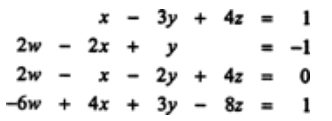
\includegraphics[width=0.35\linewidth]{img07/w07-LabExample02-eq} \end{center}

\textbf{Solution}: Performing Gaussian eliminations (i.e., the series of row operations), we have

\begin{center}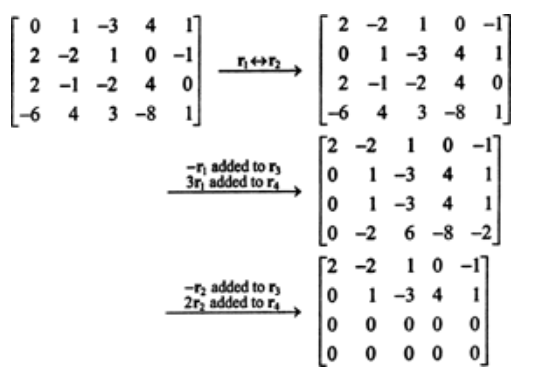
\includegraphics[width=0.55\linewidth]{img07/w07-LabExample02-sol} \end{center}

\begin{Shaded}
\begin{Highlighting}[]
\DocumentationTok{\#\#}
\NormalTok{A1 }\OtherTok{=} \FunctionTok{matrix}\NormalTok{(}\FunctionTok{c}\NormalTok{(}\DecValTok{0}\NormalTok{,}\DecValTok{1}\NormalTok{,}\SpecialCharTok{{-}}\DecValTok{3}\NormalTok{,}\DecValTok{4}\NormalTok{,}\DecValTok{1}\NormalTok{,}\DecValTok{2}\NormalTok{,}\SpecialCharTok{{-}}\DecValTok{2}\NormalTok{,}\DecValTok{1}\NormalTok{,}\DecValTok{0}\NormalTok{,}\SpecialCharTok{{-}}\DecValTok{1}\NormalTok{,}\DecValTok{2}\NormalTok{,}\SpecialCharTok{{-}}\DecValTok{1}\NormalTok{,}\SpecialCharTok{{-}}\DecValTok{2}\NormalTok{,}\DecValTok{4}\NormalTok{,}\DecValTok{0}\NormalTok{,}\SpecialCharTok{{-}}\DecValTok{6}\NormalTok{,}\DecValTok{4}\NormalTok{,}\DecValTok{3}\NormalTok{,}\SpecialCharTok{{-}}\DecValTok{8}\NormalTok{,}\DecValTok{1}\NormalTok{), }\AttributeTok{ncol =}\DecValTok{5}\NormalTok{, }\AttributeTok{byrow =} \ConstantTok{TRUE}\NormalTok{)}
\FunctionTok{Gauss.Elimination}\NormalTok{(}\AttributeTok{A =}\NormalTok{ A1)}
\end{Highlighting}
\end{Shaded}

\begin{verbatim}
##      [,1] [,2] [,3] [,4] [,5]
## [1,]    2   -2    1    0   -1
## [2,]    0    1   -3    4    1
## [3,]    0    0    0    0    0
## [4,]    0    0    0    0    0
\end{verbatim}

\hfill\break

\textbf{Example 3} Solve the following system of linear equations.

\begin{center}\includegraphics[width=0.35\linewidth]{img07/w07-LabExample03-eq} \end{center}

\textbf{Solution}: Performing Gaussian eliminations (i.e., the series of row operations), we have

\begin{center}\includegraphics[width=0.55\linewidth]{img07/w07-LabExample03-sol} \end{center}

\begin{Shaded}
\begin{Highlighting}[]
\NormalTok{A1 }\OtherTok{=} \FunctionTok{matrix}\NormalTok{(}\FunctionTok{c}\NormalTok{(}\DecValTok{1}\NormalTok{,}\DecValTok{1}\NormalTok{,}\SpecialCharTok{{-}}\DecValTok{3}\NormalTok{,}\DecValTok{4}\NormalTok{,}\DecValTok{2}\NormalTok{,}\DecValTok{1}\NormalTok{,}\SpecialCharTok{{-}}\DecValTok{1}\NormalTok{,}\DecValTok{2}\NormalTok{,}\DecValTok{3}\NormalTok{,}\DecValTok{2}\NormalTok{,}\SpecialCharTok{{-}}\DecValTok{4}\NormalTok{,}\DecValTok{7}\NormalTok{), }\AttributeTok{ncol =} \DecValTok{4}\NormalTok{, }\AttributeTok{byrow =} \ConstantTok{TRUE}\NormalTok{)}
\FunctionTok{Gauss.Elimination}\NormalTok{(}\AttributeTok{A =}\NormalTok{ A1)}
\end{Highlighting}
\end{Shaded}

\begin{verbatim}
##      [,1] [,2] [,3] [,4]
## [1,]    1    1   -3    4
## [2,]    0   -1    5   -6
## [3,]    0    0    0    1
\end{verbatim}

\hfill\break

\textbf{Example 4} Solve the following system of linear equations.

\begin{center}\includegraphics[width=0.22\linewidth]{img07/w07-LabExample04-eq} \end{center}

\textbf{Solution}: Performing Gaussian eliminations (i.e., the series of row operations), we have

\begin{center}\includegraphics[width=0.5\linewidth]{img07/w07-LabExample04-1-sol} \end{center}

\begin{Shaded}
\begin{Highlighting}[]
\NormalTok{A1 }\OtherTok{=} \FunctionTok{matrix}\NormalTok{(}\FunctionTok{c}\NormalTok{(}\DecValTok{1}\SpecialCharTok{/}\DecValTok{4}\NormalTok{, }\DecValTok{1}\SpecialCharTok{/}\DecValTok{2}\NormalTok{, }\DecValTok{1}\NormalTok{, }\DecValTok{23}\SpecialCharTok{/}\DecValTok{4}\NormalTok{, }\DecValTok{1}\NormalTok{,}\DecValTok{1}\NormalTok{,}\DecValTok{1}\NormalTok{,}\DecValTok{7}\NormalTok{,}\DecValTok{4}\NormalTok{,}\DecValTok{2}\NormalTok{,}\DecValTok{1}\NormalTok{,}\DecValTok{2}\NormalTok{), }\AttributeTok{ncol =} \DecValTok{4}\NormalTok{, }\AttributeTok{byrow =} \ConstantTok{TRUE}\NormalTok{)}
\FunctionTok{Gauss.Elimination}\NormalTok{(}\AttributeTok{A =}\NormalTok{ A1)}
\end{Highlighting}
\end{Shaded}

\begin{verbatim}
##      [,1] [,2] [,3]   [,4]
## [1,] 0.25  0.5    1   5.75
## [2,] 0.00 -1.0   -3 -16.00
## [3,] 0.00  0.0    3   6.00
\end{verbatim}

\hypertarget{gauss-jordan-elimination-optional}{%
\section{\texorpdfstring{Gauss-Jordan Elimination (\texttt{Optional})}{Gauss-Jordan Elimination (Optional)}}\label{gauss-jordan-elimination-optional}}

\begin{Shaded}
\begin{Highlighting}[]
\DocumentationTok{\#\#\#\#}
\NormalTok{Gauss.Jordan }\OtherTok{=} \ControlFlowTok{function}\NormalTok{(A)\{}
  \CommentTok{\# A is the augmented matrix}
\NormalTok{  A1 }\OtherTok{=} \FunctionTok{Gauss.Elimination}\NormalTok{(A)           }\CommentTok{\# perform Gauss elimination}
\NormalTok{  n }\OtherTok{=} \FunctionTok{length}\NormalTok{(A1[,}\DecValTok{1}\NormalTok{])}
\NormalTok{  id}\FloatTok{.0} \OtherTok{=} \FunctionTok{rep}\NormalTok{(}\DecValTok{1}\NormalTok{,n)                     }\CommentTok{\# indicator of zero A[i,i]}
  \ControlFlowTok{for}\NormalTok{ (i }\ControlFlowTok{in} \DecValTok{1}\SpecialCharTok{:}\NormalTok{n)\{}
    \ControlFlowTok{if}\NormalTok{(A1[i,i] }\SpecialCharTok{==} \DecValTok{0}\NormalTok{) id}\FloatTok{.0}\NormalTok{[i] }\OtherTok{=} \DecValTok{0}
\NormalTok{  \}}
  \ControlFlowTok{if}\NormalTok{(}\FunctionTok{sum}\NormalTok{(id}\FloatTok{.0}\NormalTok{) }\SpecialCharTok{==}\NormalTok{ n)\{                  }\CommentTok{\# A[i,i] != 0}
\NormalTok{        k }\OtherTok{=}\NormalTok{ n}
\NormalTok{        A2 }\OtherTok{=}\NormalTok{ A1[k}\SpecialCharTok{:}\DecValTok{1}\NormalTok{, }\FunctionTok{c}\NormalTok{(k}\SpecialCharTok{:}\DecValTok{1}\NormalTok{,(n}\SpecialCharTok{+}\DecValTok{1}\NormalTok{))]     }\CommentTok{\# re{-}arrange rows and columns}
\NormalTok{        A3 }\OtherTok{=} \FunctionTok{Gauss.Elimination}\NormalTok{(A2)     }\CommentTok{\# perform Gauss elimination}
\NormalTok{        A4 }\OtherTok{=}\NormalTok{ A3[k}\SpecialCharTok{:}\DecValTok{1}\NormalTok{, }\FunctionTok{c}\NormalTok{(k}\SpecialCharTok{:}\DecValTok{1}\NormalTok{,(n}\SpecialCharTok{+}\DecValTok{1}\NormalTok{))]     }\CommentTok{\# backward re{-}arrangement}
\NormalTok{      \} }\ControlFlowTok{else}\NormalTok{\{                          }\CommentTok{\# if exists A[i,i] =0}
\NormalTok{        k }\OtherTok{=} \FunctionTok{which}\NormalTok{(id}\FloatTok{.0}\SpecialCharTok{==}\DecValTok{0}\NormalTok{)[}\DecValTok{1}\NormalTok{]}\SpecialCharTok{{-}}\DecValTok{1}   \CommentTok{\# select rows and columns for re{-}arrangement}
\NormalTok{        A2 }\OtherTok{=}\NormalTok{ A1[}\FunctionTok{c}\NormalTok{(k}\SpecialCharTok{:}\DecValTok{1}\NormalTok{,(k}\SpecialCharTok{+}\DecValTok{1}\NormalTok{)}\SpecialCharTok{:}\NormalTok{n), }\FunctionTok{c}\NormalTok{(k}\SpecialCharTok{:}\DecValTok{1}\NormalTok{,(k}\SpecialCharTok{+}\DecValTok{1}\NormalTok{)}\SpecialCharTok{:}\NormalTok{(n}\SpecialCharTok{+}\DecValTok{1}\NormalTok{))]}
\NormalTok{        A3 }\OtherTok{=} \FunctionTok{Gauss.Elimination}\NormalTok{(A2)}
\NormalTok{        A4 }\OtherTok{=}\NormalTok{ A3[}\FunctionTok{c}\NormalTok{(k}\SpecialCharTok{:}\DecValTok{1}\NormalTok{,(k}\SpecialCharTok{+}\DecValTok{1}\NormalTok{)}\SpecialCharTok{:}\NormalTok{n), }\FunctionTok{c}\NormalTok{(k}\SpecialCharTok{:}\DecValTok{1}\NormalTok{,(k}\SpecialCharTok{+}\DecValTok{1}\NormalTok{)}\SpecialCharTok{:}\NormalTok{(n}\SpecialCharTok{+}\DecValTok{1}\NormalTok{))]}
\NormalTok{      \}}
\NormalTok{   A4}
\NormalTok{\}}
\end{Highlighting}
\end{Shaded}

\textbf{Example 5} (continuation of \textbf{Example 4})

We can perform additional row operations (Gaussian-Jordan) to get

\begin{center}\includegraphics[width=0.5\linewidth]{img07/w07-LabExample04-2-sol} \end{center}

\begin{Shaded}
\begin{Highlighting}[]
\NormalTok{A1 }\OtherTok{=} \FunctionTok{matrix}\NormalTok{(}\FunctionTok{c}\NormalTok{(}\DecValTok{1}\SpecialCharTok{/}\DecValTok{4}\NormalTok{, }\DecValTok{1}\SpecialCharTok{/}\DecValTok{2}\NormalTok{, }\DecValTok{1}\NormalTok{, }\DecValTok{23}\SpecialCharTok{/}\DecValTok{4}\NormalTok{, }\DecValTok{1}\NormalTok{,}\DecValTok{1}\NormalTok{,}\DecValTok{1}\NormalTok{,}\DecValTok{7}\NormalTok{,}\DecValTok{4}\NormalTok{,}\DecValTok{2}\NormalTok{,}\DecValTok{1}\NormalTok{,}\DecValTok{2}\NormalTok{), }\AttributeTok{ncol =} \DecValTok{4}\NormalTok{, }\AttributeTok{byrow =} \ConstantTok{TRUE}\NormalTok{)}
\FunctionTok{Gauss.Jordan}\NormalTok{(}\AttributeTok{A =}\NormalTok{ A1)}
\end{Highlighting}
\end{Shaded}

\begin{verbatim}
##      [,1] [,2] [,3]   [,4]
## [1,] 0.25    0    0  -1.25
## [2,] 0.00   -1    0 -10.00
## [3,] 0.00    0    3   6.00
\end{verbatim}

\hfill\break

\textbf{Example 6} (continuation of \textbf{Example 2}) Gauss-Jordan elimination

\begin{Shaded}
\begin{Highlighting}[]
\NormalTok{A6 }\OtherTok{=} \FunctionTok{matrix}\NormalTok{(}\FunctionTok{c}\NormalTok{(}\DecValTok{0}\NormalTok{,}\DecValTok{1}\NormalTok{,}\SpecialCharTok{{-}}\DecValTok{3}\NormalTok{,}\DecValTok{4}\NormalTok{,}\DecValTok{1}\NormalTok{,}\DecValTok{2}\NormalTok{,}\SpecialCharTok{{-}}\DecValTok{2}\NormalTok{,}\DecValTok{1}\NormalTok{,}\DecValTok{0}\NormalTok{,}\SpecialCharTok{{-}}\DecValTok{1}\NormalTok{,}\DecValTok{2}\NormalTok{,}\SpecialCharTok{{-}}\DecValTok{1}\NormalTok{,}\SpecialCharTok{{-}}\DecValTok{2}\NormalTok{,}\DecValTok{4}\NormalTok{,}\DecValTok{0}\NormalTok{,}\SpecialCharTok{{-}}\DecValTok{6}\NormalTok{,}\DecValTok{4}\NormalTok{,}\DecValTok{3}\NormalTok{,}\SpecialCharTok{{-}}\DecValTok{8}\NormalTok{,}\DecValTok{1}\NormalTok{), }\AttributeTok{ncol =}\DecValTok{5}\NormalTok{, }\AttributeTok{byrow =} \ConstantTok{TRUE}\NormalTok{)}
\FunctionTok{Gauss.Jordan}\NormalTok{(}\AttributeTok{A =}\NormalTok{ A6)}
\end{Highlighting}
\end{Shaded}

\begin{verbatim}
##      [,1] [,2] [,3] [,4] [,5]
## [1,]    2    0   -5    8    1
## [2,]    0    1   -3    4    1
## [3,]    0    0    0    0    0
## [4,]    0    0    0    0    0
\end{verbatim}

\hfill\break

\textbf{Example 7} (continuation of \textbf{Example 3}) Gauss-Jordan form

\begin{Shaded}
\begin{Highlighting}[]
\NormalTok{A7 }\OtherTok{=} \FunctionTok{matrix}\NormalTok{(}\FunctionTok{c}\NormalTok{(}\DecValTok{1}\NormalTok{,}\DecValTok{1}\NormalTok{,}\SpecialCharTok{{-}}\DecValTok{3}\NormalTok{,}\DecValTok{4}\NormalTok{,}\DecValTok{2}\NormalTok{,}\DecValTok{1}\NormalTok{,}\SpecialCharTok{{-}}\DecValTok{1}\NormalTok{,}\DecValTok{2}\NormalTok{,}\DecValTok{3}\NormalTok{,}\DecValTok{2}\NormalTok{,}\SpecialCharTok{{-}}\DecValTok{4}\NormalTok{,}\DecValTok{7}\NormalTok{), }\AttributeTok{ncol =} \DecValTok{4}\NormalTok{, }\AttributeTok{byrow =} \ConstantTok{TRUE}\NormalTok{)}
\FunctionTok{Gauss.Jordan}\NormalTok{(}\AttributeTok{A =}\NormalTok{ A7)}
\end{Highlighting}
\end{Shaded}

\begin{verbatim}
##      [,1] [,2] [,3] [,4]
## [1,]    1    0    2   -2
## [2,]    0   -1    5   -6
## [3,]    0    0    0    1
\end{verbatim}

\hfill\break

\textbf{Example 8} (continuation of \textbf{Example 4}) Gauss-Jordan form

\begin{Shaded}
\begin{Highlighting}[]
\NormalTok{A8 }\OtherTok{=} \FunctionTok{matrix}\NormalTok{(}\FunctionTok{c}\NormalTok{(}\DecValTok{1}\SpecialCharTok{/}\DecValTok{4}\NormalTok{, }\DecValTok{1}\SpecialCharTok{/}\DecValTok{2}\NormalTok{, }\DecValTok{1}\NormalTok{, }\DecValTok{23}\SpecialCharTok{/}\DecValTok{4}\NormalTok{, }\DecValTok{1}\NormalTok{,}\DecValTok{1}\NormalTok{,}\DecValTok{1}\NormalTok{,}\DecValTok{7}\NormalTok{,}\DecValTok{4}\NormalTok{,}\DecValTok{2}\NormalTok{,}\DecValTok{1}\NormalTok{,}\DecValTok{2}\NormalTok{), }\AttributeTok{ncol =} \DecValTok{4}\NormalTok{, }\AttributeTok{byrow =} \ConstantTok{TRUE}\NormalTok{)}
\FunctionTok{Gauss.Jordan}\NormalTok{(}\AttributeTok{A =}\NormalTok{ A8)}
\end{Highlighting}
\end{Shaded}

\begin{verbatim}
##      [,1] [,2] [,3]   [,4]
## [1,] 0.25    0    0  -1.25
## [2,] 0.00   -1    0 -10.00
## [3,] 0.00    0    3   6.00
\end{verbatim}

\hypertarget{determinant-and-inversion-of-matrices}{%
\chapter{Determinant and Inversion of Matrices}\label{determinant-and-inversion-of-matrices}}

We have introduced the Gaussian elimination method to solve the linear system of equations. This note focuses on the algorithm for finding the inverse of square matrices and then use the algorithm to solve matrix equations,

\hypertarget{concepts-of-matrix-a-review}{%
\section{Concepts of Matrix: A Review}\label{concepts-of-matrix-a-review}}

We first define some special matrices and then review the basic properties of matrices.

\hypertarget{definitions-of-some-special-matrices}{%
\subsection{Definitions of Some Special Matrices}\label{definitions-of-some-special-matrices}}

A general form of a \(n\times m\) matrix is given by

\[
A_{n\times m} = \left[\begin{array}{ccccc} 
a_{11} & a_{12} & \cdots & a_{1m}  \\ 
a_{21} & a_{22} & \cdots & a_{2m}  \\ 
\vdots & \vdots & \vdots & \vdots  \\
a_{n-1,1} & a_{n-1.2} & \cdots & a_{n-1,m}  \\
a_{n1} & a_{n2} & \cdots & a_{nm}  
\end{array}
\right]
\]

That \(n\) rows and \(m\) columns. If \(n = m\), the corresponding matrix is called the \textbf{square matrix}. If all off-diagonal elements of a square matrix are equal to zero, the square matrix is called \textbf{diagonal matrix}

\[
D_{n\times n} = \left[\begin{array}{ccccc} 
a_{11} & 0 & \cdots & 0  \\ 
0 & a_{22} & \cdots & 0  \\ 
\vdots & \vdots & \ddots & \vdots  \\
0 & 0& \cdots & a_{nn}  
\end{array}
\right]
\]
A very important special diagonal matrix with all diagonal elements being 1 is called \textbf{identity matrix} and has the following form

\[
I_{n\times n} = \left[\begin{array}{ccccc} 
1 & 0 & \cdots & 0  \\ 
0 & 1 & \cdots & 0  \\ 
\vdots & \vdots & \ddots & \vdots  \\
0 & 0& \cdots & 1  
\end{array}
\right]
\]

The following square matrix is called a symmetric matrix

\[
A_{n\times n} = \left[\begin{array}{ccccc} 
a_{11} & a_{12} & \cdots & a_{1n}  \\ 
a_{12} & a_{22} & \cdots & a_{2n}  \\ 
\vdots & \vdots & \vdots & \vdots  \\
a_{1,n-1} & a_{2,n-1} & \cdots & a_{n,n-1}  \\
a_{1n} & a_{2n} & \cdots & a_{nn}  
\end{array}
\right]
\]
A square matrix is called lower triangular if all the entries above the main diagonal are zero. Similarly, a square matrix is called upper triangular if all the entries below the main diagonal are zero. S and T represent lower and upper triangular matrices respectively.

\[
S_{n\times n} = \left[\begin{array}{ccccc} 
a_{11} & a_{12} & \cdots & a_{1n}  \\ 
0 & a_{22} & \cdots & a_{2n}  \\ 
\vdots & \vdots & \vdots & \vdots  \\
0 & 0 & \cdots & a_{nn}  
\end{array}
\right]
~
~
\text{and}
~
~
T_{n\times n} = \left[\begin{array}{ccccc} 
b_{11} & 0 & \cdots & 0  \\ 
b_{21} & b_{22} & \cdots & 0  \\ 
\vdots & \vdots & \vdots & 0  \\
b_{n1} & b_{n2} & \cdots & b_{nn}  
\end{array}
\right]
\]

\hfill\break

\hypertarget{binary-operations}{%
\subsection{Binary Operations}\label{binary-operations}}

We perform matrix addition and subtraction, the two matrices must have the same dimensions.

\hfill\break

\textbf{Addition and Subtraction}

Let

\[
A_{n\times m} = \left[\begin{array}{ccccc} 
a_{11} & a_{12} & \cdots & a_{1m}  \\ 
a_{21} & a_{22} & \cdots & a_{2m}  \\ 
\vdots & \vdots & \vdots & \vdots  \\
a_{n-1,1} & a_{n-1.2} & \cdots & a_{n-1,m}  \\
a_{n1} & a_{n2} & \cdots & a_{nm}  
\end{array}
\right]
~
~
\text{and}
~
~
B_{n\times m} = \left[\begin{array}{ccccc} 
b_{11} & b_{12} & \cdots & b_{1m}  \\ 
b_{21} & b_{22} & \cdots & b_{2m}  \\ 
\vdots & \vdots & \vdots & \vdots  \\
b_{n-1,1} & b_{n-1.2} & \cdots & b_{n-1,m}  \\
b_{n1} & b_{n2} & \cdots & b_{nm}  
\end{array}
\right]
\]

\[
A_{n\times m}\pm B_{n\times m} = \left[\begin{array}{ccccc} 
a_{11}\pm b_{11} & a_{12}\pm b_{12} & \cdots & a_{1m}\pm b_{1m}  \\ 
a_{21}\pm b_{21} & a_{21}\pm b_{22} & \cdots & a_{21}\pm b_{2m}  \\ 
\vdots & \vdots & \vdots & \vdots  \\
a_{n-1,1}\pm b_{n-1,1} & a_{n-1,1}\pm b_{n-1.2} & \cdots & a_{n-1,1}\pm b_{n-1,m}  \\
a_{n1}\pm b_{n1} & a_{n1}\pm b_{n2} & \cdots & a_{nm}\pm b_{nm}  
\end{array}
\right]
\]\\

\textbf{Multiplication}

When multiplying two matrices, the two matrices must be compatible. That is the number of \textbf{columns} of the first (left) matrix MUST be equal to the number of \textbf{rows} in the second (right) matrix. To illustrate this compatibility, we define

\[
C_{p\times q} = \left[\begin{array}{ccccc} 
c_{11} & c_{12} & \cdots & c_{1q}  \\ 
c_{21} & c_{22} & \cdots & c_{2q}  \\ 
\vdots & \vdots & \vdots & \vdots  \\
c_{p-1,1} & c_{p-1,2} & \cdots & c_{p-1,m}  \\
c_{p1} & c_{p2} & \cdots & c_{pq}  
\end{array}
\right]
~
~
\text{and}
~
~
D_{q\times k} = \left[\begin{array}{ccccc} 
d_{11} & d_{12} & \cdots & d_{1k}  \\ 
d_{21} & d_{22} & \cdots & d_{2k}  \\ 
\vdots & \vdots & \vdots & \vdots  \\
d_{q-1,1} & d_{q-1.2} & \cdots & d_{q-1kk}  \\
d_{q1} & d_{q2} & \cdots & d_{qk}  
\end{array}
\right]
\]

The product of the above two matrices is defined to be

\[
M_{p\times k} = \left[\begin{array}{ccccc} 
c_{11}\times d_{11} + c_{12}\times d_{21} + \cdots + c_{1q}\times d_{q1}  & \cdots & c_{11}\times d_{1k} + c_{12}\times d_{2k} + \cdots + c_{1q}\times d_{qk} \\ 
c_{21}\times d_{11} + c_{22}\times d_{21} + \cdots + c_{2q}\times d_{q1}  & \cdots & c_{21}\times d_{1k} + c_{22}\times d_{2k} + \cdots + c_{2q}\times d_{qk} \\ 
\vdots & \vdots & \vdots  \\
c_{p-1,1}\times d_{11} + c_{p-1,2}\times d_{21} + \cdots + c_{p-1,q}\times d_{q1}  & \cdots & c_{p-1,1}\times d_{1k} + c_{p-1,2}\times d_{2k} + \cdots + c_{p-1,q}\times d_{qk}  \\
c_{p1}\times d_{11} + c_{p2}\times d_{21} + \cdots + c_{pq}\times d_{q1}  & \cdots & c_{p1}\times d_{1k} + c_{p2}\times d_{2k} + \cdots + c_{pq}\times d_{qk}  
\end{array}
\right]
\]

In general, multiplication is NOT commutative. That is, \(A\times B \ne B\times A\).

\textbf{Example 1}: Define
\[
C_{3\times 4} = \left[\begin{array}{ccccc} 
1& 2 & 3 & 4  \\ 
4 & 3 & 2 & 1 \\ 
1 & 3 & 5 & 2  
\end{array}
\right]
~
~
\text{and}
~
~
D_{4\times 3} = \left[\begin{array}{ccccc} 
2 & 1 & 4   \\ 
3 & 2 & 2  \\ 
0 & 1 & 3  \\
1 & 2 & 5
\end{array}
\right]
\]
Then
\[
C_{3\times 4} \times D_{4\times 3} = \left[\begin{array}{ccccc} 
1& 2 & 3 & 4  \\ 
4 & 3 & 2 & 1 \\ 
1 & 3 & 5 & 2  
\end{array}
\right]
\times
\left[\begin{array}{ccccc} 
2 & 1 & 4   \\ 
3 & 2 & 2  \\ 
0 & 1 & 3  \\
1 & 2 & 5
\end{array}
\right]
~
=
~
 \left[\begin{array}{ccccc} 
12 & 16 & 37   \\ 
18 & 14 & 33  \\ 
13 & 16 & 35  \\
\end{array}
\right].
\]
However,

\[
D_{4\times 3} \times C_{3\times 4} = 
\left[\begin{array}{ccccc} 
2 & 1 & 4   \\ 
3 & 2 & 2  \\ 
0 & 1 & 3  \\
1 & 2 & 5
\end{array}
\right]
\times
\left[\begin{array}{ccccc} 
1& 2 & 3 & 4  \\ 
4 & 3 & 2 & 1 \\ 
1 & 3 & 5 & 2  
\end{array}
\right]
~
=
~
 \left[\begin{array}{ccccc} 
10 & 19 & 28 & 17 \\ 
13 & 18 & 23 & 18\\ 
7 & 12 & 17 & 7\\
14 & 23 & 32 & 16
\end{array}
\right].
\]

\hfill\break

\textbf{Division} is not defined in matrix algebra. For example, Even with two square matrices \(P_{nn}\) and \(Q_{nn}\), \(P \div Q\) is NOT defined! The concept of the inverse of a square matrix is analogous to the concept of the reciprocal of a number. The detail of the inverse matrix will be discussed in the subsequent sections.

\hfill\break

\hypertarget{unary-operations}{%
\subsection{Unary Operations}\label{unary-operations}}

Addition, subtraction, and multiplication involve two matrices. Next look at some unary operations in matrix algebra.

\textbf{Transpose}. The matrix that is resulting from a given matrix B after changing or reversing its rows to columns and columns to rows is called the transpose of a matrix B. For example,

\[
D_{3\times 4} = \left[\begin{array}{ccccc} 
1& 2 & 3 & 4  \\ 
4 & 3 & 2 & 1 \\ 
1 & 3 & 5 & 2  
\end{array}
\right]
~
~
\text{and}
~
~
D^T_{4\times 3} = \left[\begin{array}{ccccc} 
1 & 4 & 1   \\ 
2 & 3 & 3  \\ 
3 & 2 & 5  \\
4 & 1 & 2
\end{array}
\right]
\]

Note that \textbf{transpose} is defined for any matrices (square or non-square) matrices.

\textbf{Trace of A Matrix}: The trace is the sum of all diagonal elements of a \textbf{square matrix}.

\[
A_{n\times n} = \left[\begin{array}{ccccc} 
a_{11} & a_{12} & \cdots & a_{1n}  \\ 
a_{21} & a_{22} & \cdots & a_{2n}  \\ 
\vdots & \vdots & \vdots & \vdots  \\
a_{n-1,1} & a_{n-1.2} & \cdots & a_{n-1,n}  \\
a_{n1} & a_{n2} & \cdots & a_{nn}  
\end{array}
\right],
~
~
\text{then}
~
~
\text{Trace}(A_{n\times n}) = \sum_{i=1}^n a_{ii}
\]

\hypertarget{determinant-of-a-square-matrix}{%
\section{Determinant of a Square Matrix}\label{determinant-of-a-square-matrix}}

The determinant of a matrix is the scalar value or number calculated using a square matrix. The calculation of a general square matrix is not straightforward, an iterative algorithm is needed. We will not introduce these algorithms in this class. But for triangular matrices, we can use the mathematical induction method to show the following theorem

\hfill\break

\textbf{Theorem}: Let \(T_n\) be an upper triangular matrix of order \(n\).

\[
T_{n} = \left[\begin{array}{ccccc} 
a_{11} & a_{12} & \cdots & a_{1n}  \\ 
0 & a_{22} & \cdots & a_{2n}  \\ 
\vdots & \vdots & \vdots & \vdots  \\
0 & 0 & \cdots & a_{nn}  
\end{array}
\right]
\]

Let \(\text{det}(T_n)\) be the determinant of \(T_n\). Then \(\text{det}(T_n)\) is equal to the product of all the diagonal elements of \(T_n\). That is

\[
\text{det}(T_n)=\sum_{i=1}^n a_{ii}.
\]

\textbf{Sketch of Proof}: We use mathematical induction to prove this theorem.

\begin{enumerate}
\def\labelenumi{\arabic{enumi}.}
\item
  The determinant is \(a_{11}\), which is clearly also the diagonal element. That is, \(\text{det}(T_1) = a_{11}\). This establishes the induction basis.
\item
  Assume that \(\text{det}(T_k) = \sum_{i=1}^k a_{ii}\) for
  \[
  T_{k} = \left[\begin{array}{ccccc} 
  a_{11} & a_{12} & \cdots & a_{1k}  \\ 
  0 & a_{22} & \cdots & a_{2k}  \\ 
  \vdots & \vdots & \vdots & \vdots  \\
  0 & 0 & \cdots & a_{kk}  
  \end{array}
  \right].
  \]
\end{enumerate}

We now consider

\[
T_{k+1} = \left[\begin{array}{ccccc} 
a_{11} & a_{12} & \cdots & a_{1k} & a_{1,k+1} \\ 
0 & a_{22} & \cdots & a_{2k}  & a_{2,k+1} \\ 
\vdots & \vdots & \vdots & \vdots & \vdots \\
0 & 0 & \cdots & a_{kk}  & a_{k,k+1} \\
0 & 0 & \cdots & 0  & a_{k+1,k+1}
\end{array}
\right].
\]

Expanding above matrix by the \((k+1)\)-th row, we have

\[
T_{k+1} = \left[\begin{array}{ccccc} 
a_{11} & a_{12} & \cdots & a_{1k} & a_{1,k+1} \\ 
0 & a_{22} & \cdots & a_{2k}  & a_{2,k+1} \\ 
\vdots & \vdots & \vdots & \vdots & \vdots \\
0 & 0 & \cdots & a_{nk}  & a_{k,k+1} \\
0 & 0 & \cdots & 0  & a_{k+1,k+1}
\end{array}
\right]
~
=
~
a_{k+1, k+1}\times \left[\begin{array}{ccccc} 
a_{11} & a_{12} & \cdots & a_{1k}  \\ 
0 & a_{22} & \cdots & a_{2k}  \\ 
\vdots & \vdots & \vdots & \vdots  \\
0 & 0 & \cdots & a_{kk}  
\end{array}
\right].
\]

Therefore,
\[
\text{det}(T_{k+1}) = \text{det}(a_{k+1,k+1}T_k) = a_{k+1, k+1} \text{det}(T_k) = a_{k+1, k+1}\sum_{i=1}^k a_{ii} = \sum_{i=1}^{k+1} a_{ii}.
\]

This completes the proof.

\hfill\break

We have introduced the Gaussian elimination algorithm that can be used for the triangulation of a square matrix. Therefore, we can use the R function we developed earlier to find the determinant of square matrices.

\begin{Shaded}
\begin{Highlighting}[]
\NormalTok{DET }\OtherTok{=} \ControlFlowTok{function}\NormalTok{(A)\{}
  \CommentTok{\# Input A: Must be a square matrix}
\NormalTok{  A0 }\OtherTok{=}\NormalTok{ A        }
\NormalTok{  n }\OtherTok{=} \FunctionTok{dim}\NormalTok{(A0)[}\DecValTok{1}\NormalTok{]                }\CommentTok{\# number of rows}
  \ControlFlowTok{for}\NormalTok{(i }\ControlFlowTok{in} \DecValTok{1}\SpecialCharTok{:}\NormalTok{(n}\DecValTok{{-}1}\NormalTok{))\{            }\CommentTok{\# iterator fo pivot element A0[i,i]}
                                \CommentTok{\# i = 1, 2, ..., n{-}1}
      \CommentTok{\#\textasciitilde{}\textasciitilde{}\textasciitilde{}\textasciitilde{}\textasciitilde{}\textasciitilde{}\textasciitilde{}\textasciitilde{}\textasciitilde{}\textasciitilde{}\textasciitilde{}\textasciitilde{}\textasciitilde{}\textasciitilde{}\textasciitilde{}\textasciitilde{}\textasciitilde{}\textasciitilde{}\textasciitilde{}\textasciitilde{}\textasciitilde{}   Make the function robust  \textasciitilde{}\textasciitilde{}\textasciitilde{}\textasciitilde{}\textasciitilde{}\textasciitilde{}\textasciitilde{}\textasciitilde{}\textasciitilde{}\textasciitilde{}\textasciitilde{}\textasciitilde{}\textasciitilde{}\textasciitilde{}\textasciitilde{}\textasciitilde{}\textasciitilde{}\textasciitilde{}\textasciitilde{}\textasciitilde{}\textasciitilde{}\textasciitilde{}\textasciitilde{}\textasciitilde{}\textasciitilde{}\#}
      \ControlFlowTok{if}\NormalTok{(A0[i,i] }\SpecialCharTok{==} \DecValTok{0}\NormalTok{)\{}
\NormalTok{          non}\FloatTok{.0} \OtherTok{=} \FunctionTok{which}\NormalTok{(A0[,i] }\SpecialCharTok{!=} \DecValTok{0}\NormalTok{)}
              \CommentTok{\#cat("\textbackslash{}n\textbackslash{}n i =",i, ", non.0 =", non.0,". (i+1):n =", (i+1):n, ".")}
\NormalTok{              id }\OtherTok{=} \FunctionTok{intersect}\NormalTok{(non}\FloatTok{.0}\NormalTok{, (i}\SpecialCharTok{+}\DecValTok{1}\NormalTok{)}\SpecialCharTok{:}\NormalTok{n)[}\DecValTok{1}\NormalTok{] }\CommentTok{\# which() equiv to find() in MATLAB}
              \ControlFlowTok{if}\NormalTok{(}\SpecialCharTok{!}\FunctionTok{is.na}\NormalTok{(id))\{}
\NormalTok{              tempi }\OtherTok{=}\NormalTok{ A0[i,]                    }\CommentTok{\# put the i{-}th row in a place{-}holder}
\NormalTok{              A0[i,] }\OtherTok{=}\NormalTok{ A0[id,]                  }\CommentTok{\# row swapping}
\NormalTok{              A0[id,] }\OtherTok{=}\NormalTok{ tempi    }
\NormalTok{            \}}
\NormalTok{      \}}
      \CommentTok{\#\textasciitilde{}\textasciitilde{}\textasciitilde{}\textasciitilde{}\textasciitilde{}\textasciitilde{}\textasciitilde{}\textasciitilde{}\textasciitilde{}\textasciitilde{}\textasciitilde{}\textasciitilde{}\textasciitilde{}\textasciitilde{}\textasciitilde{}\textasciitilde{}\textasciitilde{}\textasciitilde{}\textasciitilde{}\textasciitilde{}\textasciitilde{}\textasciitilde{}\textasciitilde{}\textasciitilde{}\textasciitilde{}\textasciitilde{}\textasciitilde{}\textasciitilde{}\textasciitilde{}\textasciitilde{}\textasciitilde{}\textasciitilde{}\textasciitilde{}\textasciitilde{}\textasciitilde{}\textasciitilde{}\textasciitilde{}\textasciitilde{}\textasciitilde{}\textasciitilde{}\textasciitilde{}\textasciitilde{}\textasciitilde{}\textasciitilde{}\textasciitilde{}\textasciitilde{}\textasciitilde{}\textasciitilde{}\textasciitilde{}\textasciitilde{}\textasciitilde{}\textasciitilde{}\textasciitilde{}\textasciitilde{}\textasciitilde{}\textasciitilde{}\textasciitilde{}\textasciitilde{}\textasciitilde{}\textasciitilde{}\textasciitilde{}\textasciitilde{}\textasciitilde{}\textasciitilde{}\textasciitilde{}\textasciitilde{}\textasciitilde{}\textasciitilde{}\textasciitilde{}\textasciitilde{}\textasciitilde{}\textasciitilde{}\#}
       \ControlFlowTok{if}\NormalTok{(A0[i,i] }\SpecialCharTok{!=} \DecValTok{0}\NormalTok{)\{    }\CommentTok{\# A0[i,i] is in the denominator of recursive equation}
          \ControlFlowTok{for}\NormalTok{(j }\ControlFlowTok{in}\NormalTok{ (i}\SpecialCharTok{+}\DecValTok{1}\NormalTok{)}\SpecialCharTok{:}\NormalTok{n)\{  }\CommentTok{\# to make the augmented matrix in the row echelon form}
             \CommentTok{\#cat("\textbackslash{}n\textbackslash{}n j =",j,".")}
\NormalTok{             A0[j,] }\OtherTok{=}\NormalTok{ A0[j,] }\SpecialCharTok{{-}}\NormalTok{ (A0[j,i]}\SpecialCharTok{/}\NormalTok{A0[i,i])}\SpecialCharTok{*}\NormalTok{A0[i,]}
\NormalTok{           \}}
\NormalTok{        \}}
\NormalTok{      \}}
\NormalTok{     DET }\OtherTok{=} \FunctionTok{prod}\NormalTok{(}\FunctionTok{diag}\NormalTok{(A0))    }\CommentTok{\# prod() {-} vectorized multiplication, diag() extracts a[i,i]}
     \ControlFlowTok{if}\NormalTok{(}\FunctionTok{dim}\NormalTok{(A)[}\DecValTok{1}\NormalTok{] }\SpecialCharTok{!=} \FunctionTok{dim}\NormalTok{(A)[}\DecValTok{2}\NormalTok{]) \{}
        \FunctionTok{cat}\NormalTok{(}\StringTok{"}\SpecialCharTok{\textbackslash{}n\textbackslash{}n}\StringTok{Need a square matrix!"}\NormalTok{)}
\NormalTok{      \} }\ControlFlowTok{else}\NormalTok{\{}
       \FunctionTok{list}\NormalTok{(}\AttributeTok{Triangular.Metrix =} \FunctionTok{round}\NormalTok{(A0,}\DecValTok{4}\NormalTok{), }\AttributeTok{Determinant =} \FunctionTok{round}\NormalTok{(DET,}\DecValTok{4}\NormalTok{))}
\NormalTok{      \}}
\NormalTok{ \}}
\end{Highlighting}
\end{Shaded}

\textbf{Example 3}. Let

\[
A = \left[\begin{array}{cccc} 
1 & 9 & 8 & 7 \\ 
3 & 8 & 3 & 8\\ 
7 & 2 & 7 & 7\\
4 & 3 & 2 & 6
\end{array}
\right].
\]

The determinant of A can be calculated using R in the following

\begin{Shaded}
\begin{Highlighting}[]
\NormalTok{A }\OtherTok{=} \FunctionTok{matrix}\NormalTok{(}\FunctionTok{c}\NormalTok{(}\DecValTok{1}\NormalTok{,}\DecValTok{9}\NormalTok{,}\DecValTok{8}\NormalTok{,}\DecValTok{7}\NormalTok{,}\DecValTok{3}\NormalTok{,}\DecValTok{8}\NormalTok{,}\DecValTok{3}\NormalTok{,}\DecValTok{8}\NormalTok{,}\DecValTok{7}\NormalTok{,}\DecValTok{2}\NormalTok{,}\DecValTok{7}\NormalTok{,}\DecValTok{7}\NormalTok{,}\DecValTok{4}\NormalTok{,}\DecValTok{3}\NormalTok{,}\DecValTok{2}\NormalTok{,}\DecValTok{6}\NormalTok{), }\AttributeTok{ncol =} \DecValTok{4}\NormalTok{, }\AttributeTok{byrow =} \ConstantTok{TRUE}\NormalTok{)}
\FunctionTok{DET}\NormalTok{(A)}
\end{Highlighting}
\end{Shaded}

\begin{verbatim}
## $Triangular.Metrix
##      [,1] [,2]     [,3]     [,4]
## [1,]    1    9   8.0000   7.0000
## [2,]    0  -19 -21.0000 -13.0000
## [3,]    0    0  18.4211  -0.2632
## [4,]    0    0   0.0000   0.6714
## 
## $Determinant
## [1] -235
\end{verbatim}

The determinant \(det(A) = -235\).

\textbf{Example 4}: Let
\[
C_{3\times 4} = \left[\begin{array}{cccc} 
1& 2 & 3 & 4  \\ 
4 & 3 & 2 & 1 \\ 
1 & 3 & 5 & 2  
\end{array}
\right]
\]

\begin{Shaded}
\begin{Highlighting}[]
\NormalTok{C}\OtherTok{=}\FunctionTok{matrix}\NormalTok{(}\FunctionTok{c}\NormalTok{(}\DecValTok{1}\NormalTok{,}\DecValTok{2}\NormalTok{,}\DecValTok{3}\NormalTok{,}\DecValTok{4}\NormalTok{,}\DecValTok{4}\NormalTok{,}\DecValTok{3}\NormalTok{,}\DecValTok{2}\NormalTok{,}\DecValTok{1}\NormalTok{,}\DecValTok{1}\NormalTok{,}\DecValTok{3}\NormalTok{,}\DecValTok{5}\NormalTok{,}\DecValTok{2}\NormalTok{), }\AttributeTok{ncol =} \DecValTok{4}\NormalTok{, }\AttributeTok{byrow =} \ConstantTok{TRUE}\NormalTok{)}
\FunctionTok{DET}\NormalTok{(C)}
\end{Highlighting}
\end{Shaded}

\begin{verbatim}
## 
## 
## Need a square matrix!
\end{verbatim}

\hfill\break

\hypertarget{matrix-inversion}{%
\section{Matrix Inversion}\label{matrix-inversion}}

\textbf{Inverse of a square matrix} Let \(A\) be a square matrix of order \(n \times n\) and let \(I_n\) be an identity matrix of same order. If there exists a square matrix \(B\), such that \(AB = BA = I\), then the matrix \(A\) is said to be invertible. The matrix \(B\) is called inverse of \(A\), that is denoted by \(A^{-1}\).

We can use the Gauss-Jordan algorithm to find the inverse of a square matrix if the inverse exists.

\textbf{Example 5} Find the inverse of the following matrix
\[
A = \left[\begin{array}{cccc} 
1 & 3 & 3    \\ 
1 & 4 & 3  \\ 
2 & 7 & 7  \\
\end{array}
\right].
\]
\textbf{Solution}: We perform the forward and backward eliminations in the following

\begin{center}\includegraphics[width=0.99\linewidth]{img08/w08-matrixInversion} \end{center}

Therefore,
\[
A^{-1} = \left[\begin{array}{cccc} 
7 & 0 & -3    \\ 
-1 & 1 & 0  \\ 
-1 & -1 & 1  \\
\end{array}
\right].
\]

The algorithm is based on the extended augmented matrix. The following is an outline of the algorithm.

Let the following square matrix be invertible.

\[
A_{n\times n} = \left[\begin{array}{cccc} 
a_{11} & a_{12} & \cdots & a_{1n}  \\ 
a_{12} & a_{22} & \cdots & a_{2n}  \\ 
\vdots & \vdots & \ddots & \vdots  \\
a_{1n} & a_{2n} & \cdots & a_{nn}  
\end{array}
\right]
\]

The extended augmented matrix is
\[
AM_{n,2n} = \left[\begin{array}{cccccccccc} 
a_{11} & a_{12} & \cdots & a_{1n} & \text{|} & 1 & 0 & \cdots & 0 \\ 
a_{21} & a_{22} & \cdots & a_{2n}  & \text{|} & 0 & 1 & \cdots & 0 \\ 
\vdots & \vdots & \ddots & \vdots & \text{|} & \vdots & \vdots & \ddots & 0 \\
a_{n1} & a_{n2} & \cdots & a_{nn}  & \text{|} & 0 & 0 & \cdots & 1 
\end{array}
\right]_{n\times 2n}.
\]

We can use Gauss-Jordan row operations to turn the above extended augmented matrix into the following form

\[
IM_{n,2n} = \left[\begin{array}{ccccccccc} 
 1 & 0 & \cdots & 0& \text{|} & w_{11} & w_{12} & \cdots & w_{1n} \\ 
0 & 1 & \cdots & 0 & \text{|} & w_{21} & w_{22} & \cdots & w_{2n}  \\ 
\vdots & \vdots & \ddots & \vdots & \text{|} & \vdots & \vdots & \ddots & 0 \\
0 & 0 & \cdots & 1  & \text{|} &  w_{n1} & w_{n2} & \cdots & w_{nn}
\end{array}
\right]_{n\times 2n}.
\]

Then the inverse of A is given by

\[
A^{-1} = \left[\begin{array}{ccccc} 
w_{11} & w_{12} & \cdots & w_{1n} \\ 
w_{21} & w_{22} & \cdots & w_{2n}  \\ 
\vdots & \vdots & \ddots & 0 \\
w_{n1} & w_{n2} & \cdots & w_{nn}
\end{array}
\right]_{n\times 2n}.
\]

We can modify the \texttt{Gauss.Jordan()} in the previous note to get the following function to calculate the inverse matrix.

\begin{Shaded}
\begin{Highlighting}[]
\NormalTok{M.inv }\OtherTok{=} \ControlFlowTok{function}\NormalTok{(A)\{}
  \CommentTok{\# Input A: Must be a square matrix}
\NormalTok{  n }\OtherTok{=} \FunctionTok{dim}\NormalTok{(A)[}\DecValTok{1}\NormalTok{]                }\CommentTok{\# number of rows}
\NormalTok{  A0 }\OtherTok{=} \FunctionTok{cbind}\NormalTok{(A, }\FunctionTok{diag}\NormalTok{(}\FunctionTok{rep}\NormalTok{(}\DecValTok{1}\NormalTok{,n)))        }
  \DocumentationTok{\#\#}
  \ControlFlowTok{for}\NormalTok{(i }\ControlFlowTok{in} \DecValTok{1}\SpecialCharTok{:}\NormalTok{(n}\DecValTok{{-}1}\NormalTok{))\{   }\CommentTok{\# iterator fo pivot element A0[i,i], i \textless{} n.}
      \CommentTok{\#\textasciitilde{}\textasciitilde{}\textasciitilde{}\textasciitilde{}\textasciitilde{}\textasciitilde{}\textasciitilde{}\textasciitilde{}\textasciitilde{}\textasciitilde{}\textasciitilde{}\textasciitilde{}\textasciitilde{}\textasciitilde{}\textasciitilde{}\textasciitilde{}\textasciitilde{}\textasciitilde{}\textasciitilde{}\textasciitilde{}\textasciitilde{}   Make the function robust  \textasciitilde{}\textasciitilde{}\textasciitilde{}\textasciitilde{}\textasciitilde{}\textasciitilde{}\textasciitilde{}\textasciitilde{}\textasciitilde{}\textasciitilde{}\textasciitilde{}\textasciitilde{}\textasciitilde{}\textasciitilde{}\textasciitilde{}\textasciitilde{}\textasciitilde{}\textasciitilde{}\textasciitilde{}\textasciitilde{}\textasciitilde{}\textasciitilde{}\textasciitilde{}\textasciitilde{}\textasciitilde{}\#}
      \ControlFlowTok{if}\NormalTok{(A0[i,i] }\SpecialCharTok{==} \DecValTok{0}\NormalTok{)\{}
\NormalTok{          non}\FloatTok{.0} \OtherTok{=} \FunctionTok{which}\NormalTok{(A0[,i] }\SpecialCharTok{!=} \DecValTok{0}\NormalTok{)}
              \CommentTok{\#cat("\textbackslash{}n\textbackslash{}n i =",i, ", non.0 =", non.0,". (i+1):n =", (i+1):n, ".")}
\NormalTok{              id }\OtherTok{=} \FunctionTok{intersect}\NormalTok{(non}\FloatTok{.0}\NormalTok{, (i}\SpecialCharTok{+}\DecValTok{1}\NormalTok{)}\SpecialCharTok{:}\NormalTok{n)[}\DecValTok{1}\NormalTok{] }\CommentTok{\# which() equiv to find() in MATLAB}
              \ControlFlowTok{if}\NormalTok{(}\SpecialCharTok{!}\FunctionTok{is.na}\NormalTok{(id))\{}
\NormalTok{              tempi }\OtherTok{=}\NormalTok{ A0[i,]                    }\CommentTok{\# put the i{-}th row in a place{-}holder}
\NormalTok{              A0[i,] }\OtherTok{=}\NormalTok{ A0[id,]                  }\CommentTok{\# row swapping}
\NormalTok{              A0[id,] }\OtherTok{=}\NormalTok{ tempi    }
\NormalTok{            \}}
\NormalTok{        \}}
      \CommentTok{\#\textasciitilde{}\textasciitilde{}\textasciitilde{}\textasciitilde{}\textasciitilde{}\textasciitilde{}\textasciitilde{}\textasciitilde{}\textasciitilde{}\textasciitilde{}\textasciitilde{}\textasciitilde{}\textasciitilde{}\textasciitilde{}\textasciitilde{}\textasciitilde{}\textasciitilde{}\textasciitilde{}\textasciitilde{}\textasciitilde{}\textasciitilde{}\textasciitilde{}\textasciitilde{}\textasciitilde{}\textasciitilde{}\textasciitilde{}\textasciitilde{}\textasciitilde{}\textasciitilde{}\textasciitilde{}\textasciitilde{}\textasciitilde{}\textasciitilde{}\textasciitilde{}\textasciitilde{}\textasciitilde{}\textasciitilde{}\textasciitilde{}\textasciitilde{}\textasciitilde{}\textasciitilde{}\textasciitilde{}\textasciitilde{}\textasciitilde{}\textasciitilde{}\textasciitilde{}\textasciitilde{}\textasciitilde{}\textasciitilde{}\textasciitilde{}\textasciitilde{}\textasciitilde{}\textasciitilde{}\textasciitilde{}\textasciitilde{}\textasciitilde{}\textasciitilde{}\textasciitilde{}\textasciitilde{}\textasciitilde{}\textasciitilde{}\textasciitilde{}\textasciitilde{}\textasciitilde{}\textasciitilde{}\textasciitilde{}\textasciitilde{}\textasciitilde{}\textasciitilde{}\textasciitilde{}\textasciitilde{}\textasciitilde{}\#}
       \ControlFlowTok{if}\NormalTok{(A0[i,i] }\SpecialCharTok{!=} \DecValTok{0}\NormalTok{)\{    }\CommentTok{\# A0[i,i] is in the denominator of recursive equation}
          \ControlFlowTok{for}\NormalTok{(j }\ControlFlowTok{in}\NormalTok{ (i}\SpecialCharTok{+}\DecValTok{1}\NormalTok{)}\SpecialCharTok{:}\NormalTok{n)\{  }\CommentTok{\# to make the augmented matrix in the row echelon form}
             \CommentTok{\#cat("\textbackslash{}n\textbackslash{}n j =",j,".")}
\NormalTok{             A0[j,] }\OtherTok{=}\NormalTok{ A0[j,] }\SpecialCharTok{{-}}\NormalTok{ (A0[j,i]}\SpecialCharTok{/}\NormalTok{A0[i,i])}\SpecialCharTok{*}\NormalTok{A0[i,]}
\NormalTok{           \}}
\NormalTok{        \}}
\NormalTok{    \}}
\NormalTok{    A1}\OtherTok{=}\NormalTok{A0  }
\NormalTok{    n }\OtherTok{=} \FunctionTok{length}\NormalTok{(A1[,}\DecValTok{1}\NormalTok{])}
\NormalTok{    id}\FloatTok{.0} \OtherTok{=} \FunctionTok{rep}\NormalTok{(}\DecValTok{1}\NormalTok{,n)                     }\CommentTok{\# indicator of zero A[i,i]}
    \ControlFlowTok{for}\NormalTok{ (i }\ControlFlowTok{in} \DecValTok{1}\SpecialCharTok{:}\NormalTok{n)\{}
          \ControlFlowTok{if}\NormalTok{(A1[i,i] }\SpecialCharTok{==} \DecValTok{0}\NormalTok{) id}\FloatTok{.0}\NormalTok{[i] }\OtherTok{=} \DecValTok{0}
\NormalTok{        \}}
    \ControlFlowTok{if}\NormalTok{(}\FunctionTok{sum}\NormalTok{(id}\FloatTok{.0}\NormalTok{) }\SpecialCharTok{==}\NormalTok{ n)\{                        }\CommentTok{\# A[i,i] != 0}
             \ControlFlowTok{for}\NormalTok{ (i }\ControlFlowTok{in} \DecValTok{1}\SpecialCharTok{:}\NormalTok{n)\{}
\NormalTok{                    A1[i,] }\OtherTok{=}\NormalTok{ A1[i,] }\SpecialCharTok{/}\NormalTok{A1[i,i]   }\CommentTok{\# Divide each row by A1[i,i] }
\NormalTok{                   \}                           }\CommentTok{\# so that new A1[i,i] = 1.}
\NormalTok{             k }\OtherTok{=}\NormalTok{ n}
\NormalTok{            A2 }\OtherTok{=}\NormalTok{ A1[k}\SpecialCharTok{:}\DecValTok{1}\NormalTok{, }\FunctionTok{c}\NormalTok{(k}\SpecialCharTok{:}\DecValTok{1}\NormalTok{,(n}\SpecialCharTok{+}\DecValTok{1}\NormalTok{)}\SpecialCharTok{:}\NormalTok{(}\DecValTok{2}\SpecialCharTok{*}\NormalTok{n))]     }\CommentTok{\# re{-}arrange rows and columns}
           \CommentTok{\#\_\_\_\_\_\_\_\_\_\_\_\_\_\_\_\_\_\_\_\_\_\_\_\_\_\_\_\_\_\_\_\_\_\_\_\_\_\_\_\_\_\_\_\_\_\_\_\_\_\_\_\_\_\_\_\_\_\_\_\_\_\_\_\#\#}
             \ControlFlowTok{for}\NormalTok{(i }\ControlFlowTok{in} \DecValTok{1}\SpecialCharTok{:}\NormalTok{(n}\DecValTok{{-}1}\NormalTok{))\{}
                  \ControlFlowTok{if}\NormalTok{(A2[i,i] }\SpecialCharTok{!=} \DecValTok{0}\NormalTok{)\{    }\CommentTok{\# A0[i,i] is in the denominator of recursive equation}
                  \ControlFlowTok{for}\NormalTok{(j }\ControlFlowTok{in}\NormalTok{ (i}\SpecialCharTok{+}\DecValTok{1}\NormalTok{)}\SpecialCharTok{:}\NormalTok{n)\{  }\CommentTok{\# to make the augmented matrix in the row echelon form}
\NormalTok{                       A2[j,] }\OtherTok{=}\NormalTok{ A2[j,] }\SpecialCharTok{{-}}\NormalTok{ (A2[j,i]}\SpecialCharTok{/}\NormalTok{A2[i,i])}\SpecialCharTok{*}\NormalTok{A2[i,]}
\NormalTok{                       \}}
\NormalTok{                  \}}
\NormalTok{               \}}
           \CommentTok{\#{-}{-}{-}{-}{-}{-}{-}{-}{-}{-}{-}{-}{-}{-}{-}{-}{-}{-}{-}{-}{-}{-}{-}{-}{-}{-}{-}{-}{-}{-}{-}{-}{-}{-}{-}{-}{-}{-}{-}{-}{-}{-}{-}{-}{-}{-}{-}{-}{-}{-}{-}{-}{-}{-}{-}{-}{-}{-}{-}{-}{-}{-}\#\#}
\NormalTok{             A4 }\OtherTok{=}\NormalTok{ A2[k}\SpecialCharTok{:}\DecValTok{1}\NormalTok{, }\FunctionTok{c}\NormalTok{(k}\SpecialCharTok{:}\DecValTok{1}\NormalTok{,(n}\SpecialCharTok{+}\DecValTok{1}\NormalTok{)}\SpecialCharTok{:}\NormalTok{(}\DecValTok{2}\SpecialCharTok{*}\NormalTok{n))]     }\CommentTok{\# backward re{-}arrangement}
             \FunctionTok{round}\NormalTok{(A4[, (n}\SpecialCharTok{+}\DecValTok{1}\NormalTok{)}\SpecialCharTok{:}\NormalTok{(}\DecValTok{2}\SpecialCharTok{*}\NormalTok{n)],}\DecValTok{7}\NormalTok{)}
\NormalTok{           \} }\ControlFlowTok{else} \ControlFlowTok{if}\NormalTok{(}\FunctionTok{dim}\NormalTok{(A)[}\DecValTok{1}\NormalTok{] }\SpecialCharTok{!=} \FunctionTok{dim}\NormalTok{(A)[}\DecValTok{2}\NormalTok{])\{}
               \FunctionTok{cat}\NormalTok{(}\StringTok{"}\SpecialCharTok{\textbackslash{}n\textbackslash{}n}\StringTok{A square matrix is needed!"}\NormalTok{)}
\NormalTok{           \}}\ControlFlowTok{else}\NormalTok{ \{}\CommentTok{\# if exists A[i,i] =0}
             \FunctionTok{cat}\NormalTok{(}\StringTok{"The matrix is singular"}\NormalTok{)}
\NormalTok{          \}}
\NormalTok{ \}}
\end{Highlighting}
\end{Shaded}

\textbf{Example 6} (continuation of example 3) Let

\[
A = \left[\begin{array}{cccc} 
1 & 9 & 8 & 7 \\ 
3 & 8 & 3 & 8\\ 
7 & 2 & 7 & 7\\
4 & 3 & 2 & 6
\end{array}
\right].
\]

The determinant of \(A\) can be calculated using R in the following

\begin{Shaded}
\begin{Highlighting}[]
\NormalTok{A }\OtherTok{=} \FunctionTok{matrix}\NormalTok{(}\FunctionTok{c}\NormalTok{(}\DecValTok{1}\NormalTok{,}\DecValTok{9}\NormalTok{,}\DecValTok{8}\NormalTok{,}\DecValTok{7}\NormalTok{,}\DecValTok{3}\NormalTok{,}\DecValTok{8}\NormalTok{,}\DecValTok{3}\NormalTok{,}\DecValTok{8}\NormalTok{,}\DecValTok{7}\NormalTok{,}\DecValTok{2}\NormalTok{,}\DecValTok{7}\NormalTok{,}\DecValTok{7}\NormalTok{,}\DecValTok{4}\NormalTok{,}\DecValTok{3}\NormalTok{,}\DecValTok{2}\NormalTok{,}\DecValTok{6}\NormalTok{), }\AttributeTok{ncol =} \DecValTok{4}\NormalTok{, }\AttributeTok{byrow =} \ConstantTok{TRUE}\NormalTok{)}
\FunctionTok{M.inv}\NormalTok{(A)   }
\end{Highlighting}
\end{Shaded}

\begin{verbatim}
##            [,1]       [,2]       [,3]       [,4]
## [1,] -0.4893617  0.8723404  0.5319149 -1.2127660
## [2,] -0.2978723  0.7744681  0.3063830 -1.0425532
## [3,]  0.1489362 -0.1872340  0.0468085  0.0212766
## [4,]  0.4255319 -0.9063830 -0.5234043  1.4893617
\end{verbatim}

\begin{Shaded}
\begin{Highlighting}[]
\FunctionTok{solve}\NormalTok{(A)   }\CommentTok{\# calling internal function solve() for comparison!}
\end{Highlighting}
\end{Shaded}

\begin{verbatim}
##            [,1]       [,2]        [,3]       [,4]
## [1,] -0.4893617  0.8723404  0.53191489 -1.2127660
## [2,] -0.2978723  0.7744681  0.30638298 -1.0425532
## [3,]  0.1489362 -0.1872340  0.04680851  0.0212766
## [4,]  0.4255319 -0.9063830 -0.52340426  1.4893617
\end{verbatim}

\textbf{Example 7} (continuation of example 4)

\begin{Shaded}
\begin{Highlighting}[]
\NormalTok{C}\OtherTok{=}\FunctionTok{matrix}\NormalTok{(}\FunctionTok{c}\NormalTok{(}\DecValTok{1}\NormalTok{,}\DecValTok{2}\NormalTok{,}\DecValTok{3}\NormalTok{,}\DecValTok{4}\NormalTok{,}\DecValTok{4}\NormalTok{,}\DecValTok{3}\NormalTok{,}\DecValTok{2}\NormalTok{,}\DecValTok{1}\NormalTok{,}\DecValTok{1}\NormalTok{,}\DecValTok{3}\NormalTok{,}\DecValTok{5}\NormalTok{,}\DecValTok{2}\NormalTok{), }\AttributeTok{ncol =} \DecValTok{4}\NormalTok{, }\AttributeTok{byrow =} \ConstantTok{TRUE}\NormalTok{)}
\FunctionTok{M.inv}\NormalTok{(C)}
\end{Highlighting}
\end{Shaded}

\begin{verbatim}
## 
## 
## A square matrix is needed!
\end{verbatim}

\textbf{Example 8} (continuation of example 5) Find the inverse of the following matrix
\[
A = \left[\begin{array}{cccc} 
1 & 3 & 3    \\ 
1 & 4 & 3  \\ 
2 & 7 & 7  \\
\end{array}
\right].
\]

\begin{Shaded}
\begin{Highlighting}[]
\NormalTok{A}\OtherTok{=}\FunctionTok{matrix}\NormalTok{(}\FunctionTok{c}\NormalTok{(}\DecValTok{1}\NormalTok{,}\DecValTok{3}\NormalTok{,}\DecValTok{3}\NormalTok{,}\DecValTok{1}\NormalTok{,}\DecValTok{4}\NormalTok{,}\DecValTok{3}\NormalTok{,}\DecValTok{2}\NormalTok{,}\DecValTok{7}\NormalTok{,}\DecValTok{7}\NormalTok{), }\AttributeTok{ncol =} \DecValTok{3}\NormalTok{, }\AttributeTok{byrow =} \ConstantTok{TRUE}\NormalTok{)}
\FunctionTok{M.inv}\NormalTok{(A)}
\end{Highlighting}
\end{Shaded}

\begin{verbatim}
##      [,1] [,2] [,3]
## [1,]    7    0   -3
## [2,]   -1    1    0
## [3,]   -1   -1    1
\end{verbatim}

\hypertarget{matrix-factorization}{%
\chapter{Matrix Factorization}\label{matrix-factorization}}

In linear algebra, a matrix factorization is a factorization of a matrix into a product of matrices. There are differences in factorizing a matrix for different purposes. Among various ways of factorization, \textbf{lower--upper (LU)} factorization is the basic and is useful in solving linear systems. Although LU factorization works for any \(m\times n\) matrix, it is common to factorize square matrix. In this note, we only discuss LU for square matrices.

Let \(A\) be the \(n\times n\) matrix

\[
A_{n\times n} = \left[\begin{array}{ccccc} 
a_{11} & a_{12} & \cdots & a_{1n}  \\ 
a_{21} & a_{22} & \cdots & a_{2n}  \\ 
\vdots & \vdots & \ddots & \vdots  \\
a_{n1} & a_{n2} & \cdots & a_{nn}  
\end{array}
\right]
\]
\(A\) is said to have a \(LU\)-decomposition if there exists matrices \(L\) and \(U\) with the following properties:

\begin{enumerate}
\def\labelenumi{\arabic{enumi}.}
\tightlist
\item
  \(L\) is a \(n\times n\) lower triangular matrix with all diagonal entries being 1.
\end{enumerate}

\[
L_{n\times n} = \left[\begin{array}{cccc} 
1 & 0 & \cdots & 0  \\ 
l_{21} & 1 & \cdots & 0  \\ 
\vdots & \vdots & \ddots & \vdots  \\
l_{n1} & l_{n2} & \cdots & 1  
\end{array}
\right]
\]

\begin{enumerate}
\def\labelenumi{\arabic{enumi}.}
\setcounter{enumi}{1}
\tightlist
\item
  \(U\) is a \(n\times n\) matrix in some echelon form.
\end{enumerate}

\[
U_{n\times n} = \left[\begin{array}{ccccc} 
u_{11} & u_{12} & \cdots & u_{1n}  \\ 
0 & u_{22} & \cdots & u_{2n}  \\ 
\vdots & \vdots & \ddots & \vdots  \\
0 & 0 & \cdots & u_{nn}  
\end{array}
\right]
\]

\begin{enumerate}
\def\labelenumi{\arabic{enumi}.}
\setcounter{enumi}{2}
\tightlist
\item
  \(A = LU\).
\end{enumerate}

\[
A_{n\times n} = \left[\begin{array}{ccccc} 
a_{11} & a_{12} & \cdots & a_{1n}  \\ 
a_{21} & a_{22} & \cdots & a_{2n}  \\ 
\vdots & \vdots & \ddots & \vdots  \\
a_{n1} & a_{n2} & \cdots & a_{nn}  
\end{array}
\right]
~
=~
\left[\begin{array}{ccccc} 
1 & 0 & \cdots & 0  \\ 
l_{21} & 1 & \cdots & 0  \\ 
\vdots & \vdots & \ddots & \vdots  \\
l_{n1} & l_{n2} & \cdots & 1  
\end{array}
\right]
\times
\left[\begin{array}{ccccc} 
u_{11} & u_{12} & \cdots & u_{1n}  \\ 
0 & u_{22} & \cdots & u_{2n}  \\ 
\vdots & \vdots & \ddots & \vdots  \\
0 & 0 & \cdots & u_{nn}  
\end{array}
\right]
~=~
L_{n\times n}\times U_{n\times n}
\]\\

\hypertarget{elementary-and-permutation-matrices}{%
\section{Elementary and Permutation Matrices}\label{elementary-and-permutation-matrices}}

Any \textbf{elementary matrix}, which we often denote by \(E\), is obtained from applying \textbf{one} row operation to the \textbf{identity matrix} of the same size.

\textbf{Examples} Consider the resulting matrices after row operations to the identity matrix.

\begin{enumerate}
\def\labelenumi{\arabic{enumi}.}
\tightlist
\item
  Adding one row to the other row: \(R_1 + R_2 \to R_2\)
\end{enumerate}

\[
E_1 = \left[\begin{array}{ccccc} 
1 & 0 &  0  \\ 
1 & 1 & 0  \\ 
0 & 0 & 1  
\end{array}
\right]
\]

\begin{enumerate}
\def\labelenumi{\arabic{enumi}.}
\setcounter{enumi}{1}
\tightlist
\item
  Multiplying a scalar to a row: \(3\times R2 \to R_2\)
\end{enumerate}

\[
E_2 = \left[\begin{array}{ccccc} 
1 & 0 &  0  \\ 
1 & 3 & 0  \\ 
0 & 0 & 1  
\end{array}
\right]
\]

\begin{enumerate}
\def\labelenumi{\arabic{enumi}.}
\setcounter{enumi}{2}
\tightlist
\item
  Multiplying a scalar to a Row and then adding it to the other row: \(5\times R_1 + R3 \to R_3\)
\end{enumerate}

\[
E_3 = \left[\begin{array}{ccccc} 
1 & 0 &  0  \\ 
0 & 1 & 0  \\ 
5 & 0 & 1  
\end{array}
\right]
\]

\begin{enumerate}
\def\labelenumi{\arabic{enumi}.}
\setcounter{enumi}{3}
\tightlist
\item
  Switching two rows: \(R_1 \leftrightarrow R_2\):
\end{enumerate}

\[
E_3 = \left[\begin{array}{ccccc} 
0 & 1 &  0  \\ 
1 & 0 & 0  \\ 
0 & 0 & 1  
\end{array}
\right]
\]

The elementary matrix obtained from switching two rows is commonly called \textbf{permutation matrix}.

\hfill\break

\textbf{\color{red}\LARGE To perform any of the first three row-operations on a matrix \(A\), it suffices to take the product (left-multiplication) \(E\times A\), where \(E\) is the elementary matrix obtained by using the desired row operation on the identity matrix.}

\hfill\break

Note that row operations (row switching) were used in matrix inversion and triangulation.

\textbf{Example 1}: Consider the triangulation problem:

\[
A= \left[\begin{array}{ccccc} 
1 & 4 & 1   \\ 
2 & 3 & 3  \\ 
3 & 2 & 5  
\end{array}
\right]
\]
\textbf{Solution}: The following three steps will complete the triangulation.

(1). \(-2\times R_1 + R_2 \to R_2\):

\[
A= \left[\begin{array}{ccccc} 
1 & 4 & 1   \\ 
2 & 3 & 3  \\ 
3 & 2 & 5  
\end{array}
\right]
~
\xrightarrow{-2\times R_1 + R_2 \to R_2}
~
A_1= \left[\begin{array}{ccccc} 
1 & 4 & 1   \\ 
0 & -5 & 1  \\ 
3 & 2 & 5  
\end{array}
\right],
~~
E_1 =\left[\begin{array}{ccccc} 
1 & 0 & 0   \\ 
-2 & 1 & 0  \\ 
0 & 0 & 1  
\end{array}
\right]
\]
Note that

\[
E_1\times A = \left[\begin{array}{ccccc} 
1 & 0 & 0   \\ 
-2 & 1 & 0  \\ 
0 & 0 & 1  
\end{array}
\right]
\times
\left[\begin{array}{ccccc} 
1 & 4 & 1   \\ 
2 & 3 & 3  \\ 
3 & 2 & 5  
\end{array}
\right]
~=~
\left[\begin{array}{ccccc} 
1 & 4 & 1   \\ 
0 & -5 & 1  \\ 
3 & 2 & 5  
\end{array}
\right]
\]

(2). \(-3\times R_1 + R_3 \to R_3\):

\[
A_1= \left[\begin{array}{ccccc} 
1 & 4 & 1   \\ 
0 & -5 & 1  \\ 
3 & 2 & 5  
\end{array}
\right]
~
\xrightarrow{-3\times R_1 + R_3 \to R_3}
~
A_2= \left[\begin{array}{ccccc} 
1 & 4 & 1   \\ 
0 & -5 & 1  \\ 
0 & -10 & 2  
\end{array}
\right],
~~
E_2 =\left[\begin{array}{ccccc} 
1 & 0 & 0   \\ 
0 & 1 & 0  \\ 
-3 & 0 & 1  
\end{array}
\right]
\]

Note also that
\[
E_2\times E_1\times A = E_2\times A_1 = \left[\begin{array}{ccccc} 
1 & 0 & 0   \\ 
0 & 1 & 0  \\ 
-3 & 0 & 1  
\end{array}
\right]
\times
\left[\begin{array}{ccccc} 
1 & 4 & 1   \\ 
0 & -5 & 1  \\ 
3 & 2 & 5  
\end{array}
\right]
~=~
\left[\begin{array}{ccccc} 
1 & 4 & 1   \\ 
0 & -5 & 1  \\ 
0 & -10 & 2  
\end{array}
\right] = A_2
\]

(3). \(-2\times R_1 + R_3 \to R_3\):

\[
A_2= \left[\begin{array}{ccccc} 
1 & 4 & 1   \\ 
0 & -5 & 1  \\ 
0 & -10 & 2  
\end{array}
\right]
~
\xrightarrow{-3\times R_1 + R_3 \to R_3}
~
A_3= \left[\begin{array}{ccccc} 
1 & 4 & 1   \\ 
0 & -5 & 1  \\ 
0 & 0 & 0  
\end{array}
\right],
~~
E_3 =\left[\begin{array}{ccccc} 
1 & 0 & 0   \\ 
0 & 1 & 0  \\ 
0 & -2 & 1  
\end{array}
\right]
\]

We note similarly that

\[
E_3\times E_2\times E_1\times A = E_3\times A_2 =\left[\begin{array}{cccc} 
1 & 0 & 0   \\ 
0 & 1 & 0  \\ 
0 & -2 & 1  
\end{array}
\right]
\times
\left[\begin{array}{cccc} 
1 & 4 & 1   \\ 
0 & -5 & 1  \\ 
0 & -10 & 2  
\end{array}
\right]
~=~
\left[\begin{array}{cccc} 
1 & 4 & 1   \\ 
0 & -5 & 1  \\ 
0 & 0 & 0  
\end{array}
\right] = A_3
\]
Next, we look at the product of the three (lower angular) elementary matrices.

\[
E = E_3\times E_2 \times E_1 =  
\left[\begin{array}{ccccc} 
1 & 0 & 0   \\ 
0 & 1 & 0  \\ 
0 & -2 & 1  
\end{array}
\right]
\times
\left[\begin{array}{ccc} 
1 & 0 & 0   \\ 
0 & 1 & 0  \\ 
-3 & 0 & 1  
\end{array}
\right]
\times
\left[\begin{array}{ccc} 
1 & 0 & 0   \\ 
-2 & 1 & 0  \\ 
0 & 0 & 1  
\end{array}
\right]
~=~
\left[\begin{array}{ccc} 
1 & 0 & 0   \\ 
-2 & 1 & 0  \\ 
1 & -2 & 1  
\end{array}
\right]
\]

Several important observations help develop algorithms to perform the \(LU\) factorization.

\begin{enumerate}
\def\labelenumi{\arabic{enumi}.}
\item
  All elementary matrices that are based on the forward row operations (NOT the row-swapping) are \textbf{lower triangular matrices} (and are obviously non-singular).
\item
  The product of all \textbf{lower triangular matrices} will also be a \textbf{lower triangular matrix}. This can easily be proved by the definition of matrix multiplication.
\item
  The product of elementary matrices is \textbf{non-singular} (i.e., the determinant is NOT equal to zero).
\item
  The inverse of a \textbf{lower triangular matrix} (if exists) is also a lower triangular. This is also obvious from the process of finding the inverse of a function
\end{enumerate}

\hfill\break

In the above example, \(A_3\) is an upper triangular matrix (special echelon form). We now rewrite the row operations in the following

\[
E\times A = \left[\begin{array}{cccc} 
1 & 0 & 0   \\ 
-2 & 1 & 0  \\ 
1 & -2 & 1  
\end{array}
\right]
\times
\left[\begin{array}{cccc} 
1 & 4 & 1   \\ 
2 & 3 & 3  \\ 
3 & 2 & 5  
\end{array}
\right]
~
=
~
\left[\begin{array}{cccc} 
1 & 4 & 1   \\ 
0 & -5 & 1  \\ 
0 & 0 & 0  
\end{array}
\right] = A_3
\]
This implies that

\[
A =
\left[\begin{array}{cccc} 
1 & 4 & 1   \\ 
2 & 3 & 3  \\ 
3 & 2 & 5  
\end{array}
\right]
~
=
~
\left[\begin{array}{cccc} 
1 & 0 & 0   \\ 
-2 & 1 & 0  \\ 
1 & -2 & 1  
\end{array}
\right]^{-1}
\times
\left[\begin{array}{cccc} 
1 & 4 & 1   \\ 
0 & -5 & 1  \\ 
0 & 0 & 0  
\end{array}
\right] = E^{-1}\times A_3
\]

Let \(L = E^{-1}\) (lower triangular matrix) and \(U = A_3\). Then \(A = LU\)! For a \(3 \times 3\) matrix, we need to perform \(3(3-1)/2 = 3\) row operations, which means, we need to take the product 3 elementary matrices to obtain the upper triangular matrix \(A_3\). The calculation of \(E\) is tedious and time-consuming. However, we can use the R function \texttt{Gauss.Elimination()} on an arguments matrix to get E.

\[
\left[\begin{array}{ccccccc} 
1 & 4 & 1 & \vdots & 1 & 0 & 0  \\ 
2 & 3 & 3 & \vdots & 0 & 1 & 0  \\  
3 & 2 & 5 & \vdots & 0 & 0 & 1    
\end{array}
\right]
\xrightarrow{\text{Gaussian Row Elimination}}
\left[\begin{array}{cccccccc} 
1 & 4 & 1  & \vdots & 1 & 0 & 0  \\ 
0 & -5 & 1 & \vdots &-2 & 1 & 0  \\  
0 & 0 & 0  & \vdots & 1 & -2 & 1    
\end{array}
\right]
\]

Using the code we developed in the earlier note to find the \(E=E_3E_2E_1\) (order is important!)

\begin{Shaded}
\begin{Highlighting}[]
\NormalTok{Gauss.Elimination }\OtherTok{=} \ControlFlowTok{function}\NormalTok{(A)\{}
  \CommentTok{\# Input A: an n{-}by{-}m matrix }
\NormalTok{  n }\OtherTok{=} \FunctionTok{dim}\NormalTok{(A)[}\DecValTok{1}\NormalTok{]         }\CommentTok{\# number of rows}
\NormalTok{  A0 }\OtherTok{=} \FunctionTok{cbind}\NormalTok{(A, }\FunctionTok{diag}\NormalTok{(}\FunctionTok{rep}\NormalTok{(}\DecValTok{1}\NormalTok{,n)))   }\CommentTok{\# Extended augmented matrix}
  \CommentTok{\#P = diag(rep(1,n))     \# identity matrix for permutation}
  \ControlFlowTok{for}\NormalTok{(i }\ControlFlowTok{in} \DecValTok{1}\SpecialCharTok{:}\NormalTok{(n}\DecValTok{{-}1}\NormalTok{))\{     }\CommentTok{\# iterator fo pivot element A0[i,i]}
                         \CommentTok{\# i = 1, 2, ..., n{-}1}
      \CommentTok{\#\textasciitilde{}\textasciitilde{}\textasciitilde{}\textasciitilde{}\textasciitilde{}\textasciitilde{}\textasciitilde{}\textasciitilde{}\textasciitilde{}\textasciitilde{}\textasciitilde{}\textasciitilde{}\textasciitilde{}\textasciitilde{}\textasciitilde{}\textasciitilde{}\textasciitilde{}\textasciitilde{}\textasciitilde{}\textasciitilde{}\textasciitilde{}   Make the function robust  \textasciitilde{}\textasciitilde{}\textasciitilde{}\textasciitilde{}\textasciitilde{}\textasciitilde{}\textasciitilde{}\textasciitilde{}\textasciitilde{}\textasciitilde{}\textasciitilde{}\textasciitilde{}\textasciitilde{}\textasciitilde{}\textasciitilde{}\textasciitilde{}\textasciitilde{}\textasciitilde{}\textasciitilde{}\textasciitilde{}\textasciitilde{}\textasciitilde{}\textasciitilde{}\textasciitilde{}\textasciitilde{}\#}
      \ControlFlowTok{if}\NormalTok{(A0[i,i] }\SpecialCharTok{==} \DecValTok{0}\NormalTok{)\{}
\NormalTok{          non}\FloatTok{.0} \OtherTok{=} \FunctionTok{which}\NormalTok{(A0[,i] }\SpecialCharTok{!=} \DecValTok{0}\NormalTok{)     }\CommentTok{\# which() equiv to find() in MATLAB}
              \CommentTok{\#cat("\textbackslash{}n\textbackslash{}n i =",i, ", non.0 =", non.0,". (i+1):n =", (i+1):n, ".")}
\NormalTok{              id }\OtherTok{=} \FunctionTok{intersect}\NormalTok{(non}\FloatTok{.0}\NormalTok{, (i}\SpecialCharTok{+}\DecValTok{1}\NormalTok{)}\SpecialCharTok{:}\NormalTok{n)[}\DecValTok{1}\NormalTok{] }\CommentTok{\# vector of common row ID in the}
                                                \CommentTok{\# lower triangular part of the matrix.}
              \ControlFlowTok{if}\NormalTok{(}\SpecialCharTok{!}\FunctionTok{is.na}\NormalTok{(id))\{     }\CommentTok{\# if the common vector is not empty, do row{-}swapping!}
\NormalTok{              tempi }\OtherTok{=}\NormalTok{ A0[i,]                    }\CommentTok{\# put the i{-}th row in a place{-}holder}
\NormalTok{              A0[i,] }\OtherTok{=}\NormalTok{ A0[id,]                  }\CommentTok{\# row swapping}
\NormalTok{              A0[id,] }\OtherTok{=}\NormalTok{ tempi    }
              \DocumentationTok{\#\#\#                               \# updating permutation matrix}
              \CommentTok{\#tempP = P[i,]}
              \CommentTok{\#P[i,] = P[id,]                    }
              \CommentTok{\#P[id,] = tempP }
\NormalTok{             \}}
\NormalTok{       \}}
      \CommentTok{\#\textasciitilde{}\textasciitilde{}\textasciitilde{}\textasciitilde{}\textasciitilde{}\textasciitilde{}\textasciitilde{}\textasciitilde{}\textasciitilde{}\textasciitilde{}\textasciitilde{}\textasciitilde{}\textasciitilde{}\textasciitilde{}\textasciitilde{}\textasciitilde{}\textasciitilde{}\textasciitilde{}\textasciitilde{}\textasciitilde{}\textasciitilde{}\textasciitilde{}\textasciitilde{}\textasciitilde{}\textasciitilde{}\textasciitilde{}\textasciitilde{}\textasciitilde{}\textasciitilde{}\textasciitilde{}\textasciitilde{}\textasciitilde{}\textasciitilde{}\textasciitilde{}\textasciitilde{}\textasciitilde{}\textasciitilde{}\textasciitilde{}\textasciitilde{}\textasciitilde{}\textasciitilde{}\textasciitilde{}\textasciitilde{}\textasciitilde{}\textasciitilde{}\textasciitilde{}\textasciitilde{}\textasciitilde{}\textasciitilde{}\textasciitilde{}\textasciitilde{}\textasciitilde{}\textasciitilde{}\textasciitilde{}\textasciitilde{}\textasciitilde{}\textasciitilde{}\textasciitilde{}\textasciitilde{}\textasciitilde{}\textasciitilde{}\textasciitilde{}\textasciitilde{}\textasciitilde{}\textasciitilde{}\textasciitilde{}\textasciitilde{}\textasciitilde{}\textasciitilde{}\textasciitilde{}\textasciitilde{}\textasciitilde{}\#}
       \ControlFlowTok{if}\NormalTok{(A0[i,i] }\SpecialCharTok{!=} \DecValTok{0}\NormalTok{)\{    }\CommentTok{\# A0[i,i] is in the denominator of recursive equation}
          \ControlFlowTok{for}\NormalTok{(j }\ControlFlowTok{in}\NormalTok{ (i}\SpecialCharTok{+}\DecValTok{1}\NormalTok{)}\SpecialCharTok{:}\NormalTok{n)\{  }\CommentTok{\# to make the augmented matrix in the row echelon form}
             \CommentTok{\#cat("\textbackslash{}n\textbackslash{}n j =",j,".")}
\NormalTok{             A0[j,] }\OtherTok{=}\NormalTok{ A0[j,] }\SpecialCharTok{{-}}\NormalTok{ (A0[j,i]}\SpecialCharTok{/}\NormalTok{A0[i,i])}\SpecialCharTok{*}\NormalTok{A0[i,]}
\NormalTok{           \}}
\NormalTok{        \}}
\NormalTok{      \}}
\NormalTok{   A0 }
\NormalTok{ \}}
\end{Highlighting}
\end{Shaded}

\begin{Shaded}
\begin{Highlighting}[]
\NormalTok{A}\OtherTok{=}\FunctionTok{matrix}\NormalTok{(}\FunctionTok{c}\NormalTok{(}\DecValTok{1}\NormalTok{,}\DecValTok{4}\NormalTok{,}\DecValTok{1}\NormalTok{,}\DecValTok{2}\NormalTok{,}\DecValTok{3}\NormalTok{,}\DecValTok{3}\NormalTok{,}\DecValTok{3}\NormalTok{,}\DecValTok{2}\NormalTok{,}\DecValTok{5}\NormalTok{), }\AttributeTok{nrow=}\DecValTok{3}\NormalTok{, }\AttributeTok{byrow =} \ConstantTok{TRUE}\NormalTok{)}
\FunctionTok{Gauss.Elimination}\NormalTok{(}\AttributeTok{A=}\NormalTok{A)}
\end{Highlighting}
\end{Shaded}

\begin{verbatim}
##      [,1] [,2] [,3] [,4] [,5] [,6]
## [1,]    1    4    1    1    0    0
## [2,]    0   -5    1   -2    1    0
## [3,]    0    0    0    1   -2    1
\end{verbatim}

\begin{center}\includegraphics[width=0.75\linewidth]{img09/w09-LU-Example} \end{center}

\begin{Shaded}
\begin{Highlighting}[]
\NormalTok{A}\OtherTok{=}\FunctionTok{matrix}\NormalTok{(}\FunctionTok{c}\NormalTok{(}\DecValTok{1}\NormalTok{,}\DecValTok{4}\NormalTok{,}\DecValTok{1}\NormalTok{,}\DecValTok{2}\NormalTok{,}\DecValTok{3}\NormalTok{,}\DecValTok{3}\NormalTok{,}\DecValTok{3}\NormalTok{,}\DecValTok{2}\NormalTok{,}\DecValTok{5}\NormalTok{), }\AttributeTok{nrow=}\DecValTok{3}\NormalTok{, }\AttributeTok{byrow =} \ConstantTok{TRUE}\NormalTok{)}
\NormalTok{B}\OtherTok{=}\FunctionTok{cbind}\NormalTok{(A, }\FunctionTok{diag}\NormalTok{(}\FunctionTok{rep}\NormalTok{(}\DecValTok{1}\NormalTok{,}\DecValTok{3}\NormalTok{)))}
\NormalTok{C }\OtherTok{=} \FunctionTok{Gauss.Elimination}\NormalTok{(B)}
\NormalTok{U }\OtherTok{=}\NormalTok{ C[,}\DecValTok{1}\SpecialCharTok{:}\DecValTok{3}\NormalTok{]}
\NormalTok{L }\OtherTok{=} \FunctionTok{solve}\NormalTok{(C[,}\DecValTok{4}\SpecialCharTok{:}\DecValTok{6}\NormalTok{])}
\NormalTok{LU }\OtherTok{=}\NormalTok{ L}\SpecialCharTok{\%*\%}\NormalTok{U}
\end{Highlighting}
\end{Shaded}

\begin{Shaded}
\begin{Highlighting}[]
\FunctionTok{pander}\NormalTok{(LU)}
\end{Highlighting}
\end{Shaded}

\begin{longtable}[]{@{}
  >{\centering\arraybackslash}p{(\columnwidth - 4\tabcolsep) * \real{0.0556}}
  >{\centering\arraybackslash}p{(\columnwidth - 4\tabcolsep) * \real{0.0556}}
  >{\centering\arraybackslash}p{(\columnwidth - 4\tabcolsep) * \real{0.0556}}@{}}
\toprule\noalign{}
\endhead
\bottomrule\noalign{}
\endlastfoot
1 & 4 & 1 \\
2 & 3 & 3 \\
3 & 2 & 5 \\
\end{longtable}

\begin{Shaded}
\begin{Highlighting}[]
\FunctionTok{pander}\NormalTok{(A)}
\end{Highlighting}
\end{Shaded}

\begin{longtable}[]{@{}
  >{\centering\arraybackslash}p{(\columnwidth - 4\tabcolsep) * \real{0.0556}}
  >{\centering\arraybackslash}p{(\columnwidth - 4\tabcolsep) * \real{0.0556}}
  >{\centering\arraybackslash}p{(\columnwidth - 4\tabcolsep) * \real{0.0556}}@{}}
\toprule\noalign{}
\endhead
\bottomrule\noalign{}
\endlastfoot
1 & 4 & 1 \\
2 & 3 & 3 \\
3 & 2 & 5 \\
\end{longtable}

\begin{center}\includegraphics[width=0.75\linewidth]{img09/w09-LU-Example00} \end{center}

\hfill\break

\hypertarget{lu-factorization-algorithm}{%
\section{LU Factorization Algorithm}\label{lu-factorization-algorithm}}

It took three elementary row operations to obtain the lower triangular matrix in the above special \(3times 3\) matrix. In general, for an \(n\times n\) matrix, we need \(n(n-1)/2\) forward row operations (excluding row-swapping) to get the upper triangular matrix.

\hfill\break

\hypertarget{row-operations-with-row-swapping}{%
\subsection{Row Operations with Row Swapping}\label{row-operations-with-row-swapping}}

As explained in the illustrative example, we can apply the Gaussian elimination method to the extended augmented matrix to obtain the product of the elementary matrices induced from the corresponding row operations if no row-swapping is involved. To be more specific, let

\[
A_{n\times n} = \left[\begin{array}{ccccc} 
a_{11} & a_{12} & \cdots & a_{1n}  \\ 
a_{21} & a_{22} & \cdots & a_{2n}  \\ 
\vdots & \vdots & \ddots & \vdots  \\
a_{n1} & a_{n2} & \cdots & a_{nn}  
\end{array}
\right],
\]

we define an extended augmented matrix in the following

\[
A^0_{n\times n} = \left[\begin{array}{ccccccccc} 
a_{11} & a_{12} & \cdots & a_{1n} & | & 1 & 0 & \cdots 0 \\ 
a_{21} & a_{22} & \cdots & a_{2n} & | & 0 & 1 & \cdots 0 \\ 
\vdots & \vdots & \ddots & \vdots & | & \vdots & \ddots & \vdots \\
a_{n1} & a_{n2} & \cdots & a_{nn} & | & 0 & 0 & \cdots 1   
\end{array}
\right],
\]

After finishing the Gaussian elimination, we have upper triangular and lower triangular matrices that are similar to those in the example.

\hfill\break

\hypertarget{row-operations-with-row-swapping-1}{%
\subsection{Row Operations with Row-swapping}\label{row-operations-with-row-swapping-1}}

When the row operation involves row-swapping (permutations), say, \(P_1, P_2, \cdots, P_k\), we need to calculate \(P=P_k\times P_{k-1}\times \cdots \times P_2\times P_1\). Then we can apply the Gaussian elimination to \(PA\) to factorize it into the product of an upper triangular matrix and a lower triangular matrix.

Note that, the linear system \(AX = B\) is equivalent to linear system \(PAX = B\) since \(P\) involves only row-swapping.

\textbf{Properties of Permutation Matrix}. Let P be a permutation matrix, then

\begin{enumerate}
\def\labelenumi{\arabic{enumi}.}
\item
  The inverse of P exists.
\item
  The inverse of P is equal to the transpose of P. \(P^{-1} = P^T\).
\end{enumerate}

\hfill\break

\hypertarget{lu-algorithm}{%
\subsection{LU ALgorithm}\label{lu-algorithm}}

\begin{verbatim}
INPUT: The input n-by-m matrix A

OUTPUT:  L, U, P (if P = I, no permutation involved)

STEP 1: Initialization: 
        n = #rows, 
        A0 = [A,I]       (extended augmented matrix)
        P = I            (n-by-n)

STEP 2: FOR i = 1 TO n DO:     (running through pivot elements)
        STEP 3: IF A[i,i] = 0 for some i DO:
                row-swapping and updating P
                ENDIF
        STEP 4: FOR j = 1 TO n DO:
                A0[j,] = A0[j,] - (A0[j,i]/A0[i,i])*A0[i,]
                ENDFOR
        ENDFOR
STEP 5: Extract P, U = A0[,1:n], L = inverse of A0[, (n+1):2n] 
STEP 6: RETURN A, P, PA, L, U.  
\end{verbatim}

\hfill\break

\textbf{R function for LU factorization}

\begin{Shaded}
\begin{Highlighting}[]
\NormalTok{LU }\OtherTok{=} \ControlFlowTok{function}\NormalTok{(A)\{}
  \CommentTok{\# Input A: an n{-}by{-}m matrix }
\NormalTok{  n }\OtherTok{=} \FunctionTok{dim}\NormalTok{(A)[}\DecValTok{1}\NormalTok{]          }\CommentTok{\# number of rows}
\NormalTok{  A0 }\OtherTok{=} \FunctionTok{cbind}\NormalTok{(A,}\FunctionTok{diag}\NormalTok{(}\FunctionTok{rep}\NormalTok{(}\DecValTok{1}\NormalTok{,n)))                 }\CommentTok{\# Extended augmented matrix}
\NormalTok{  P }\OtherTok{=} \FunctionTok{diag}\NormalTok{(}\FunctionTok{rep}\NormalTok{(}\DecValTok{1}\NormalTok{,n))     }\CommentTok{\# identity matrix for permutation}
\NormalTok{  E }\OtherTok{=} \FunctionTok{diag}\NormalTok{(}\FunctionTok{rep}\NormalTok{(}\DecValTok{1}\NormalTok{,n))     }\CommentTok{\# for the elementary matrix involving no row exchange.}
  \ControlFlowTok{for}\NormalTok{(i }\ControlFlowTok{in} \DecValTok{1}\SpecialCharTok{:}\NormalTok{(n}\DecValTok{{-}1}\NormalTok{))\{     }\CommentTok{\# iterator fo pivot element A0[i,i]}
                         \CommentTok{\# i = 1, 2, ..., n{-}1}
         \CommentTok{\#\textasciitilde{}\textasciitilde{}\textasciitilde{}\textasciitilde{}\textasciitilde{}\textasciitilde{}\textasciitilde{}\textasciitilde{}\textasciitilde{}\textasciitilde{}\textasciitilde{}\textasciitilde{}\textasciitilde{}\textasciitilde{}\textasciitilde{}\textasciitilde{}\textasciitilde{}\textasciitilde{}\textasciitilde{}\textasciitilde{}\textasciitilde{}   Make the function robust  \textasciitilde{}\textasciitilde{}\textasciitilde{}\textasciitilde{}\textasciitilde{}\textasciitilde{}\textasciitilde{}\textasciitilde{}\textasciitilde{}\textasciitilde{}\textasciitilde{}\textasciitilde{}\textasciitilde{}\textasciitilde{}\textasciitilde{}\textasciitilde{}\textasciitilde{}\textasciitilde{}\textasciitilde{}\textasciitilde{}\textasciitilde{}\textasciitilde{}\textasciitilde{}\textasciitilde{}\textasciitilde{}\#}
         \ControlFlowTok{if}\NormalTok{(A0[i,i] }\SpecialCharTok{==} \DecValTok{0}\NormalTok{)\{}
\NormalTok{            non}\FloatTok{.0} \OtherTok{=} \FunctionTok{which}\NormalTok{(A0[,i] }\SpecialCharTok{!=} \DecValTok{0}\NormalTok{)     }\CommentTok{\# which() equiv to find() in MATLAB}
              \CommentTok{\#cat("\textbackslash{}n\textbackslash{}n i =",i, ", non.0 =", non.0,". (i+1):n =", (i+1):n, ".")}
\NormalTok{              id }\OtherTok{=} \FunctionTok{intersect}\NormalTok{(non}\FloatTok{.0}\NormalTok{, (i}\SpecialCharTok{+}\DecValTok{1}\NormalTok{)}\SpecialCharTok{:}\NormalTok{n)[}\DecValTok{1}\NormalTok{] }\CommentTok{\# vector of common row ID in the}
                                                \CommentTok{\# lower triangular part of the matrix.}
              \ControlFlowTok{if}\NormalTok{(}\SpecialCharTok{!}\FunctionTok{is.na}\NormalTok{(id))\{     }\CommentTok{\# if the common vector is not empty, do row{-}swapping!}
\NormalTok{              tempi }\OtherTok{=}\NormalTok{ A0[i,]                    }\CommentTok{\# put the i{-}th row in a place{-}holder}
\NormalTok{              A0[i,] }\OtherTok{=}\NormalTok{ A0[id,]                  }\CommentTok{\# row swapping}
\NormalTok{              A0[id,] }\OtherTok{=}\NormalTok{ tempi    }
              \DocumentationTok{\#\#\#                               \# updating permutation matrix}
\NormalTok{              tempP }\OtherTok{=}\NormalTok{ P[i,]}
\NormalTok{              P[i,] }\OtherTok{=}\NormalTok{ P[id,]                    }
\NormalTok{              P[id,] }\OtherTok{=}\NormalTok{ tempP }
\NormalTok{            \}}
\NormalTok{           \}}
        \CommentTok{\#\textasciitilde{}\textasciitilde{}\textasciitilde{}\textasciitilde{}\textasciitilde{}\textasciitilde{}\textasciitilde{}\textasciitilde{}\textasciitilde{}\textasciitilde{}\textasciitilde{}\textasciitilde{}\textasciitilde{}\textasciitilde{}\textasciitilde{}\textasciitilde{}\textasciitilde{}\textasciitilde{}\textasciitilde{}\textasciitilde{}\textasciitilde{}\textasciitilde{}\textasciitilde{}\textasciitilde{}\textasciitilde{}\textasciitilde{}\textasciitilde{}\textasciitilde{}\textasciitilde{}\textasciitilde{}\textasciitilde{}\textasciitilde{}\textasciitilde{}\textasciitilde{}\textasciitilde{}\textasciitilde{}\textasciitilde{}\textasciitilde{}\textasciitilde{}\textasciitilde{}\textasciitilde{}\textasciitilde{}\textasciitilde{}\textasciitilde{}\textasciitilde{}\textasciitilde{}\textasciitilde{}\textasciitilde{}\textasciitilde{}\textasciitilde{}\textasciitilde{}\textasciitilde{}\textasciitilde{}\textasciitilde{}\textasciitilde{}\textasciitilde{}\textasciitilde{}\textasciitilde{}\textasciitilde{}\textasciitilde{}\textasciitilde{}\textasciitilde{}\textasciitilde{}\textasciitilde{}\textasciitilde{}\textasciitilde{}\textasciitilde{}\textasciitilde{}\textasciitilde{}\textasciitilde{}\textasciitilde{}\textasciitilde{}\#}
        \ControlFlowTok{if}\NormalTok{(A0[i,i] }\SpecialCharTok{!=} \DecValTok{0}\NormalTok{)\{     }\CommentTok{\# A0[i,i] is in the denominator of recursive equation}
        \ControlFlowTok{for}\NormalTok{(j }\ControlFlowTok{in}\NormalTok{ (i}\SpecialCharTok{+}\DecValTok{1}\NormalTok{)}\SpecialCharTok{:}\NormalTok{n)\{    }\CommentTok{\# to make the augmented matrix in the row echelon form}
             \CommentTok{\#cat("\textbackslash{}n\textbackslash{}n j =",j,".")}
\NormalTok{             A0[j,] }\OtherTok{=}\NormalTok{ A0[j,] }\SpecialCharTok{{-}}\NormalTok{ (A0[j,i]}\SpecialCharTok{/}\NormalTok{A0[i,i])}\SpecialCharTok{*}\NormalTok{A0[i,]}
\NormalTok{             E[j,] }\OtherTok{=}\NormalTok{ E[j,] }\SpecialCharTok{{-}}\NormalTok{ (A0[j,i]}\SpecialCharTok{/}\NormalTok{A0[i,i])}\SpecialCharTok{*}\NormalTok{E[i,]}
\NormalTok{            \}}
\NormalTok{        \}}
       \CommentTok{\#print(E)}
\NormalTok{     \}}
\NormalTok{   PA }\OtherTok{=}\NormalTok{ P}\SpecialCharTok{\%*\%}\NormalTok{A}
\NormalTok{   U }\OtherTok{=}\NormalTok{ A0[,}\DecValTok{1}\SpecialCharTok{:}\NormalTok{n]}
\NormalTok{   L }\OtherTok{=} \FunctionTok{solve}\NormalTok{(A0[,(n}\SpecialCharTok{+}\DecValTok{1}\NormalTok{)}\SpecialCharTok{:}\NormalTok{(}\DecValTok{2}\SpecialCharTok{*}\NormalTok{n)])}
\NormalTok{   A }\OtherTok{=}\NormalTok{ A}
   \FunctionTok{list}\NormalTok{(}\AttributeTok{A =}\NormalTok{ A, }\AttributeTok{P =}\NormalTok{ P, }\AttributeTok{PA =}\NormalTok{ PA, }\AttributeTok{L =}\NormalTok{ L, }\AttributeTok{U =}\NormalTok{ U)}
\NormalTok{ \}}
\end{Highlighting}
\end{Shaded}

\hfill\break

\textbf{Example 2}

\begin{Shaded}
\begin{Highlighting}[]
\NormalTok{A}\OtherTok{=}\FunctionTok{matrix}\NormalTok{(}\FunctionTok{c}\NormalTok{(}\DecValTok{0}\NormalTok{,}\DecValTok{0}\NormalTok{,}\SpecialCharTok{{-}}\DecValTok{1}\NormalTok{, }\DecValTok{1}\NormalTok{, }\DecValTok{1}\NormalTok{, }\DecValTok{1}\NormalTok{, }\SpecialCharTok{{-}}\DecValTok{1}\NormalTok{, }\DecValTok{2}\NormalTok{, }\SpecialCharTok{{-}}\DecValTok{1}\NormalTok{, }\SpecialCharTok{{-}}\DecValTok{1}\NormalTok{, }\DecValTok{2}\NormalTok{, }\DecValTok{0}\NormalTok{, }\DecValTok{1}\NormalTok{, }\DecValTok{2}\NormalTok{, }\DecValTok{0}\NormalTok{, }\DecValTok{2}\NormalTok{), }\AttributeTok{ncol  =} \DecValTok{4}\NormalTok{, }\AttributeTok{byrow =} \ConstantTok{TRUE}\NormalTok{)}
\FunctionTok{LU}\NormalTok{(A)}
\end{Highlighting}
\end{Shaded}

\begin{verbatim}
## $A
##      [,1] [,2] [,3] [,4]
## [1,]    0    0   -1    1
## [2,]    1    1   -1    2
## [3,]   -1   -1    2    0
## [4,]    1    2    0    2
## 
## $P
##      [,1] [,2] [,3] [,4]
## [1,]    0    1    0    0
## [2,]    0    0    0    1
## [3,]    0    0    1    0
## [4,]    1    0    0    0
## 
## $PA
##      [,1] [,2] [,3] [,4]
## [1,]    1    1   -1    2
## [2,]    1    2    0    2
## [3,]   -1   -1    2    0
## [4,]    0    0   -1    1
## 
## $L
##      [,1] [,2] [,3] [,4]
## [1,]    0    0   -1    1
## [2,]    1    0    0    0
## [3,]   -1    0    1    0
## [4,]    1    1    0    0
## 
## $U
##      [,1] [,2] [,3] [,4]
## [1,]    1    1   -1    2
## [2,]    0    1    1    0
## [3,]    0    0    1    2
## [4,]    0    0    0    3
\end{verbatim}

\hypertarget{benefit-of-lu-factorization}{%
\section{Benefit of LU Factorization}\label{benefit-of-lu-factorization}}

Suppose that \(A\) has been factored into the triangular form \(A = LU\), where \(L\) is lower triangular and \(U\) is upper triangular. Then we can solve for x more easily by using a two-step process.

\begin{itemize}
\item
  Let \(y = Ux\) and solve the lower triangular system \(Ly = b\) for \(y\). Since \(L\) is triangular, determining \(y\) from this equation requires only \(O(n^2)\) operations.
\item
  Once \(y\) is known, the upper triangular system \(Ux = y\) requires only an additional \(O(n^2)\) operations to determine the solution \(x\).
\end{itemize}

Solving a linear system \(Ax = b\) in factored form means that the number of operations needed to solve the system \(Ax = b\) is reduced from \(O(n^3/3)\) to \(O(2n^2)\).

\hypertarget{least-square-approximation}{%
\chapter{Least Square Approximation}\label{least-square-approximation}}

We have introduced the direct methods in matrix algebra and several interpolation methods to approximate a univariate function with either an explicitly given analytic expression or with an unknown expression. In this note, we use matrix algebra to approximate an unknown linear and some nonlinear functions with multiple variables.

\hfill\break

\hypertarget{concepts-of-least-square-approximation}{%
\section{Concepts of Least Square Approximation}\label{concepts-of-least-square-approximation}}

To get a better idea of the least square approximation, we start with a linear approximation with only a single variable.

\begin{itemize}
\item
  \textbf{The Linear Function to Approximate}: \(y = f(x) =\beta_0 + \beta_1 x\). \(\beta_0\) and \(\beta_1\) are unknown and will be estimated from the given information.
\item
  \textbf{Given Information}: A set of data points \(\{(x_1, y_1), (x_2, y_2), \cdots, (x_n, y_n)\}\).
\end{itemize}

The idea is to find \(\hat{\beta}_0\) and \(\hat{\beta}_1\) based on the given data points that \textbf{MINIMIZES} the mean square error (MSE) between the predicted second coordinate \(\hat{y}_i = \hat{\beta}_0 + \hat{\beta}_1 x_i\) and the observed \(y_i\). To be more specific,

\begin{enumerate}
\def\labelenumi{\arabic{enumi}.}
\item
  Assume that the hypothetical linear function has analytic expression \(y = \beta_0 + \beta_1 x\).
\item
  Define the predicted to be \(\hat{y}_i = \beta_0 + \beta_1 x_i\).
\item
  Define error \(d_i = \hat{y}_i - y_i\).
\item
  Define MSE as
  \[
  \text{MSE}(\beta_0, \beta_1) = \frac{\sum_{i=1}^n d_i^2}{n-2}
  \]
\end{enumerate}

The LSE estimates the unknowns \(\beta_0\) and \(\beta_1\) by minimizing the MSE!

\url{https://github.com/pengdsci/MAT325/raw/main/w14/img/w14-best-fit-line.gif}

\hfill\break

\hypertarget{approximating-one-variable-linear-function}{%
\section{Approximating One-variable Linear Function}\label{approximating-one-variable-linear-function}}

To approximate \(\beta_0\) and \(\beta_1\), we minimize MSE defined in the previous section in the following. Denote \(Q(\beta_0, \beta_1) = \sum_{i =1}^n d_i^2 = \sum_{i =1}^n (y_i - \beta_0 - \beta_1 x_i )^2\). The approximated \(\beta_0\) and \(\beta_1\), denoted by \(\hat{\beta}_0\) and \(\hat{\beta}_1\), is the solution to the following optimization problem

\[
\text{arg min}_{\beta_0, \beta_1} Q(\beta_0, \beta_1)
\]

To minimize \(Q(\beta_0, \beta_1)\), we find the first-order derivatives and set them to zero.

\[
\frac{\partial Q(\beta_0, \beta_1)}{\partial \beta_0} = -\sum_{i=1}^n (y_i-\beta_0 - \beta_1 x_i) =0,\\
\frac{\partial Q(\beta_0, \beta_1)}{\partial \beta_1} = -\sum_{i=1}^n (y_i-\beta_0 - \beta_1 x_i)x_i=0.
\]

The above system is equivalent to

\[
\begin{array}{rclcl}
n\beta_0 & + & (\sum_{i=1}^n x_i)\beta_1 & = & \sum_{i=1}^n y_i, \\
(\sum_{i=1}^nx_i)\beta_0 &  + &(\sum_{i=1}^nx_i^2)\beta_1& = &\sum_{i=1}^n x_iy_i.
\end{array}
\]

The matrix representation of the above system is given by

\[
\left[
\begin{array}{cc}
 n               & \sum_{i=1}^n x_i \\
 \sum_{i=1}^nx_i & \sum_{i=1}^nx_i^2
\end{array}
\right]
\left[
\begin{array}{c}
\beta_0 \\
\beta_1
\end{array}
\right]
~~=~~
\left[
\begin{array}{c}
\sum_{i=1}^n y_i \\
\sum_{i=1}^n x_iy_i
\end{array}
\right],
\]

which can be further re-expressed as

\[
\left[
\begin{array}{cccccc}
 1 & 1 &\cdots & 1 & 1 \\
 x_1 & x_2 & \cdots & x_{n-1} & x_n \\
\end{array}
\right]
\left[
\begin{array}{cc}
 1 & x_1 \\
 1 & x_2 \\
 \vdots & \vdots \\
 1 & x_{n-1}\\
 1 & x_n \\
\end{array}
\right]
\left[
\begin{array}{c}
\beta_0 \\
\beta_1
\end{array}
\right]
~~=~~
\left[
\begin{array}{cccccc}
 1 & 1 &\cdots & 1 & 1 \\
 x_1 & x_2 & \cdots & x_{n-1} & x_n \\
\end{array}
\right]
\left[
\begin{array}{c}
y_1 \\
y_2\\
\vdots\\
y_{n-1}\\
y_n
\end{array}
\right].
\]

Denote
\[
\mathbf{X} =
\left[
\begin{array}{cc}
 1 & x_1 \\
 1 & x_2 \\
 \vdots & \vdots \\
 1 & x_{n-1} \\
 1 & x_n
\end{array}
\right],
~~~
\mathbf{Y} =
\left[
\begin{array}{c}
y_1 \\
y_2\\
\vdots\\
y_{n-1}\\
y_n
\end{array}
\right],
~~\text{and}~~
\mathbf{\beta} =
\left[
\begin{array}{c}
\beta_0 \\
\beta_1
\end{array}
\right].
\]
Then

\[
\mathbf{X}^T \mathbf{X} \mathbf{\beta} = \mathbf{X}^T\mathbf{Y}.
\]

Clearly, \(\mathbf{X}^T \mathbf{X}\) is a square matrix. If it is invertible, we solve for \(\mathbf{\beta}\) from the above system
\[
\mathbf{\beta} = [\mathbf{X}^T \mathbf{X}]^{-1} \mathbf{X}^T\mathbf{Y}.
\]
The right-hand side of the above equation is only dependent on the given data points. Therefore, \(\mathbf{\hat{\beta}} = [\mathbf{X}^T \mathbf{X}]^{-1} \mathbf{X}^T\mathbf{Y}\) is the solution to the minimization problem.

Therefore, \(\hat{y} = \hat{\beta}_0 + \hat{\beta}_1 x\) is the least square approximation of \(y = \beta_0 + \beta_1 x\).

\hfill\break

\textbf{Example 1}: The data are from \(n = 214\) females in statistics classes at the University of California at Davis (\url{https://raw.githubusercontent.com/pengdsci/MAT325/main/w14/LS-ApproxHeights.txt}). The variables are \(y = \text{student’s self-reported height}\), \(x_1 = \text{student’s guess at her mother’s height}\), and \(x_2 = \text{student’s guess at her father’s height}\). All heights are in inches. The scatter plots below are of each student's height versus the mother's height and the student's height against the father's height.

\begin{Shaded}
\begin{Highlighting}[]
\NormalTok{height }\OtherTok{=} \FunctionTok{read.table}\NormalTok{(}\StringTok{"https://raw.githubusercontent.com/pengdsci/MAT325/main/w14/LS{-}ApproxHeights.txt"}\NormalTok{, }\AttributeTok{header =} \ConstantTok{TRUE}\NormalTok{)  }\CommentTok{\# read data }
\NormalTok{studentHeight }\OtherTok{=}\NormalTok{ height}\SpecialCharTok{$}\NormalTok{Height    }\CommentTok{\# extract students\textquotesingle{} heights from the data set and store them in a numeric vector}
\NormalTok{momHeight }\OtherTok{=}\NormalTok{ height}\SpecialCharTok{$}\NormalTok{momheight     }\CommentTok{\# vector of mothers\textquotesingle{} heights}
\NormalTok{dadHeight }\OtherTok{=}\NormalTok{ height}\SpecialCharTok{$}\NormalTok{dadheight     }\CommentTok{\# vector of fathers\textquotesingle{} heights}
\DocumentationTok{\#\# making scatter plots}
\FunctionTok{par}\NormalTok{(}\AttributeTok{mfrow =} \FunctionTok{c}\NormalTok{(}\DecValTok{1}\NormalTok{,}\DecValTok{2}\NormalTok{))              }\CommentTok{\# setting up the layout of the graphical page}
\FunctionTok{plot}\NormalTok{(momHeight, studentHeight, }\AttributeTok{pch =} \DecValTok{19}\NormalTok{, }\AttributeTok{col =} \StringTok{"blue"}\NormalTok{, }\AttributeTok{main =} \StringTok{""}\NormalTok{)}
\FunctionTok{plot}\NormalTok{(dadHeight, studentHeight, }\AttributeTok{pch =} \DecValTok{19}\NormalTok{, }\AttributeTok{col =} \StringTok{"darkred"}\NormalTok{, }\AttributeTok{main =} \StringTok{""}\NormalTok{)}
\end{Highlighting}
\end{Shaded}

\begin{center}\includegraphics{MAT325EB_files/figure-latex/unnamed-chunk-164-1} \end{center}

\textbf{Solution}: We want to approximate the linear relationship between students' heights and their mothers' and fathers' heights respectively.

\emph{Part I}: Assume that the linear function between students' heights and their mothers' heights is of the following form

\[
y= \beta_0 + \beta_1 x_1
\]
To approximate \(\beta_0\) and \(\beta_1\), we define \(\mathbf{X}\) and \(\mathbf{Y}\) and then find the solution of the LS approximation in the following R code.

\begin{Shaded}
\begin{Highlighting}[]
\NormalTok{n }\OtherTok{=} \FunctionTok{length}\NormalTok{(studentHeight)}
\NormalTok{X }\OtherTok{=} \FunctionTok{cbind}\NormalTok{(}\FunctionTok{rep}\NormalTok{(}\DecValTok{1}\NormalTok{,n), momHeight)}
\NormalTok{Y }\OtherTok{=} \FunctionTok{cbind}\NormalTok{(studentHeight)}
\NormalTok{beta }\OtherTok{=} \FunctionTok{round}\NormalTok{(}\FunctionTok{solve}\NormalTok{(}\FunctionTok{t}\NormalTok{(X)}\SpecialCharTok{\%*\%}\NormalTok{X)}\SpecialCharTok{\%*\%}\NormalTok{(}\FunctionTok{t}\NormalTok{(X)}\SpecialCharTok{\%*\%}\NormalTok{Y),}\DecValTok{4}\NormalTok{)}
\FunctionTok{kable}\NormalTok{(beta)}
\end{Highlighting}
\end{Shaded}

\begin{tabular}{l|r}
\hline
  & studentHeight\\
\hline
 & 34.0223\\
\hline
momHeight & 0.4834\\
\hline
\end{tabular}

Therefore, the linear function is approximated by \(y = 34.0223 + 0.4834x_1\).

\hfill\break

\hypertarget{approximating-multiple-variable-linear-function}{%
\section{Approximating Multiple-variable Linear Function}\label{approximating-multiple-variable-linear-function}}

\hypertarget{an-extension-of-the-height-example}{%
\subsection{An Extension of the Height Example}\label{an-extension-of-the-height-example}}

In the above example, we assume that a student's height is only dependent on her mother's height. However, the height of a person is dependent on both parents. We further assume that the relationship has form \(y = \beta_0 + \beta_1 x_1 + \beta_2 x_2\). Then we need to approximate unknowns \((\beta_0, \beta_1, \beta_2\) using the same logic that was used for approximating the linear function with only a single variable. To be more specific, we need only to modify the matrix of \(\mathbf{X}\) by adding one additional column. The three matrices for

\[
\mathbf{X} =
\left[
\begin{array}{ccc}
 1 & x_{11} & x_{21} \\
 1 & x_{12} & x_{22} \\
 \vdots & \vdots \\
 1 & x_{1,n-1} & x_{2, n-1} \\
 1 & x_{1n} & x_{2n}
\end{array}
\right],
~~~
\mathbf{Y} =
\left[
\begin{array}{c}
y_1 \\
y_2\\
\vdots\\
y_{n-1}\\
y_n
\end{array}
\right],
~~\text{and}~~
\mathbf{\beta} =
\left[
\begin{array}{c}
\beta_0 \\
\beta_1 \\
\beta_2
\end{array}
\right].
\]

The LS approximation of \((\beta_0, \beta_1, \beta_2)\) is given by

\[
\mathbf{\beta} = [\mathbf{X}^T \mathbf{X}]^{-1} \mathbf{X}^T\mathbf{Y}.
\]

\hfill\break

\textbf{Example 2} {[}Continuation of \emph{Example 1}{]}. We now approximate linear function \(y = \beta_0 + \beta_1 x_1 + \beta x_2\) using the data given in example 1. The following R code approximates the coefficients of the linear function.

\begin{Shaded}
\begin{Highlighting}[]
\NormalTok{height }\OtherTok{=} \FunctionTok{read.table}\NormalTok{(}\StringTok{"https://raw.githubusercontent.com/pengdsci/MAT325/main/w14/LS{-}ApproxHeights.txt"}\NormalTok{, }\AttributeTok{header =} \ConstantTok{TRUE}\NormalTok{)  }\CommentTok{\# read data }
\NormalTok{studentHeight }\OtherTok{=}\NormalTok{ height}\SpecialCharTok{$}\NormalTok{Height    }\CommentTok{\# extract students\textquotesingle{} heights from the data set and store them in a numeric vector}
\NormalTok{momHeight }\OtherTok{=}\NormalTok{ height}\SpecialCharTok{$}\NormalTok{momheight     }\CommentTok{\# vector of mothers\textquotesingle{} heights}
\NormalTok{dadHeight }\OtherTok{=}\NormalTok{ height}\SpecialCharTok{$}\NormalTok{dadheight     }\CommentTok{\# vector of fathers\textquotesingle{} heights}
\NormalTok{n }\OtherTok{=} \FunctionTok{length}\NormalTok{(studentHeight)}
\NormalTok{X }\OtherTok{=} \FunctionTok{cbind}\NormalTok{(}\FunctionTok{rep}\NormalTok{(}\DecValTok{1}\NormalTok{,n), momHeight, dadHeight)}
\NormalTok{Y }\OtherTok{=} \FunctionTok{cbind}\NormalTok{(studentHeight)}
\NormalTok{beta }\OtherTok{=} \FunctionTok{round}\NormalTok{(}\FunctionTok{solve}\NormalTok{(}\FunctionTok{t}\NormalTok{(X)}\SpecialCharTok{\%*\%}\NormalTok{X)}\SpecialCharTok{\%*\%}\NormalTok{(}\FunctionTok{t}\NormalTok{(X)}\SpecialCharTok{\%*\%}\NormalTok{Y),}\DecValTok{4}\NormalTok{)}
\FunctionTok{kable}\NormalTok{(beta)}
\end{Highlighting}
\end{Shaded}

\begin{tabular}{l|r}
\hline
  & studentHeight\\
\hline
 & 18.5473\\
\hline
momHeight & 0.3035\\
\hline
dadHeight & 0.3879\\
\hline
\end{tabular}

Therefore, the approximated linear function is \(y = 18.55 + 0.3035x_1 + 0.3879x_2\).

\hfill\break

\hypertarget{approximating-general-multi-variables-linear-functions}{%
\subsection{Approximating General Multi-variables Linear Functions}\label{approximating-general-multi-variables-linear-functions}}

To approximate linear function \(y = \beta_0 + \beta_1x_1 + \beta_2x_2 + \cdots = \beta_kx_k\) based on a set of given data points \((y_i, x_{1i}, x_{2i}, \cdots, x_{ki})\) for \(i = 1, 2, \cdots, n\), we extend the \(\mathbf{X}\) matrix similarly by adding more columns to it based on the given data points. To be more specific, the three matrices used in the LS approximation are explicitly given by

\[
\mathbf{X} =
\left[
\begin{array}{ccccc}
 1 & x_{11} & x_{21} & \cdots & x_{k1} \\
 1 & x_{12} & x_{22} & \cdots & x_{k2}\\
 \vdots & \vdots & \ddots & \vdots &\vdots\\
 1 & x_{1,n-1} & x_{2, n-1} & \cdots & x_{k,n-1}\\
 1 & x_{1n} & x_{2n} & \cdots & x_{kn}
\end{array}
\right],
~~~
\mathbf{Y} =
\left[
\begin{array}{c}
y_1 \\
y_2\\
\vdots\\
y_{n-1}\\
y_n
\end{array}
\right],
~~\text{and}~~
\mathbf{\beta} =
\left[
\begin{array}{c}
\beta_0 \\
\beta_1 \\
\beta_2 \\
\vdots \\
\beta_{k-1}\\
\beta_k
\end{array}
\right].
\]

The solution to the LS approximation has the same general form given below

\[
\mathbf{\beta} = [\mathbf{X}^T \mathbf{X}]^{-1} \mathbf{X}^T\mathbf{Y}.
\]

\textbf{Example 3}: For a sample of \(n = 20\) individuals, we have measurements of \(y = \text{body fat}\), \(x_1 = \text{triceps skinfold thickness}\), \$x\_2 = text\{thigh circumference\}, and \(x_3 = \text{midarm circumference}\). The Data can be found at \url{https://raw.githubusercontent.com/pengdsci/MAT325/main/w14/LS-Approximation-Bodyfat.txt}.

\textbf{Solution} We use the following code to find the approximated coefficients in the linear function \(y = \beta_0 + \beta_1 x_1 + \beta_2 x_2 + \beta_3 x_3\).

\begin{Shaded}
\begin{Highlighting}[]
\NormalTok{bodyFat }\OtherTok{=} \FunctionTok{read.table}\NormalTok{(}\StringTok{"https://raw.githubusercontent.com/pengdsci/MAT325/main/w14/LS{-}Approximation{-}Bodyfat.txt"}\NormalTok{, }\AttributeTok{header =} \ConstantTok{TRUE}\NormalTok{)}
\NormalTok{n }\OtherTok{=} \FunctionTok{dim}\NormalTok{(bodyFat)[}\DecValTok{1}\NormalTok{]   }\CommentTok{\# number of data points}
\NormalTok{X }\OtherTok{=} \FunctionTok{as.matrix}\NormalTok{(}\FunctionTok{cbind}\NormalTok{(}\AttributeTok{intercept=}\FunctionTok{rep}\NormalTok{(}\DecValTok{1}\NormalTok{,n), bodyFat[, }\DecValTok{1}\SpecialCharTok{:}\DecValTok{3}\NormalTok{]))}
\NormalTok{Y }\OtherTok{=} \FunctionTok{as.matrix}\NormalTok{(bodyFat[,}\DecValTok{4}\NormalTok{])}
\NormalTok{beta }\OtherTok{=} \FunctionTok{round}\NormalTok{(}\FunctionTok{solve}\NormalTok{(}\FunctionTok{t}\NormalTok{(X)}\SpecialCharTok{\%*\%}\NormalTok{X)}\SpecialCharTok{\%*\%}\NormalTok{(}\FunctionTok{t}\NormalTok{(X)}\SpecialCharTok{\%*\%}\NormalTok{Y),}\DecValTok{4}\NormalTok{)}
\FunctionTok{kable}\NormalTok{(beta)}
\end{Highlighting}
\end{Shaded}

\begin{tabular}{l|r}
\hline
intercept & 117.0847\\
\hline
Triceps & 4.3341\\
\hline
Thigh & -2.8568\\
\hline
Midarm & -2.1861\\
\hline
\end{tabular}

Therefore, the approximated linear function is \(y = 117.1 + 4.334x_1 - 2.857 x_2 - 2.186 x_3\), or equivalently, \(\text{body fat} = 117.1 + 4.334\text{Tricps} - 2.857 \text{Thigh} - 2.186 \text{Midarm}\).

\hfill\break

\hypertarget{approximating-one-variable-polynomial-function}{%
\section{Approximating One-variable Polynomial Function}\label{approximating-one-variable-polynomial-function}}

We have introduced several interpolation-based approximations to a function. In this section, we use the LS approach to approximate a single variable polynomial. \(y = a_0 + a_1 x + a_2x^2 + \cdots + a_kx^k\).

\hfill\break

\hypertarget{approximating-quadratic-function}{%
\subsection{Approximating Quadratic Function}\label{approximating-quadratic-function}}

As an illustrative example, let's approximate the trend line of the sales of a particular brand of vehicles. \(\text{sales} = f(\text{time})\), the variable \textbf{time} represents the number of weeks.

\begin{center}\includegraphics[width=0.35\linewidth]{img14/w14-CarSaleTrendLine} \end{center}

The scatter plot of the two variables is given below.

\begin{center}\includegraphics{MAT325EB_files/figure-latex/unnamed-chunk-169-1} \end{center}

The above plot indicates a non-linear trend. A quadratic trend seems to be more appropriate to characterize the relationship.

Assuming the quadratic relation between the time and the sales, we have the unknown quadratic function \(\text{sales} = f(\text{time}) = a_0 + a_1 \text{time} + a_2\text{time}^2\). If we denote \(y = \text{sales}\), \(x_1 = \text{time}\), and \(x_2 = \text{time}^2\), the unknown quadratic function can written as \(y = a_0 + a_1x_1 +a_2x_2\). This means we can still use the multi-variable LS to approximate the unknown quadratic function. To be more specific, matrices \(\mathbf{X}\) and \(\mathbf{Y}\) for the LS approximation are given by

\[
\mathbf{X} = \left[
\begin{array}{ccc}
1  &  168  &  28224  \\
1  &  428  &  183184  \\
1  &  296  &  87616  \\
1  &  392  &  153664  \\
1  &  80  &  6400  \\
1  &  56  &  3136  \\
1  &  352  &  123904  \\
1  &  444  &  197136  \\
1  &  168  &  28224  \\
1  &  200  &  40000\\
1  &  4  &  16  \\
1  &  52  &  2704  \\
1  &  20  &  400  \\
1  &  228  &  51984  \\
1  &  72  &  5184
\end{array}
\right]
~~~~
\mathbf{Y} =\left[
\begin{array}{c}
272\\
300\\
311\\
365\\
167\\
149\\
366\\
310\\
192\\
229\\
88\\
118\\
62\\
319\\
193
\end{array}
\right]
\]

The coefficients of the quadratic function are estimated by

\[
\mathbf{\beta} = [\mathbf{X}^T \mathbf{X}]^{-1} \mathbf{X}^T\mathbf{Y}.
\]
The following R code calculates the approximated coefficients.

\begin{Shaded}
\begin{Highlighting}[]
\NormalTok{Y }\OtherTok{=} \FunctionTok{matrix}\NormalTok{(}\FunctionTok{c}\NormalTok{(}\DecValTok{272}\NormalTok{, }\DecValTok{300}\NormalTok{, }\DecValTok{311}\NormalTok{, }\DecValTok{365}\NormalTok{, }\DecValTok{167}\NormalTok{, }\DecValTok{149}\NormalTok{, }\DecValTok{366}\NormalTok{, }\DecValTok{310}\NormalTok{, }\DecValTok{192}\NormalTok{, }\DecValTok{229}\NormalTok{, }\DecValTok{88}\NormalTok{, }\DecValTok{118}\NormalTok{, }\DecValTok{62}\NormalTok{, }\DecValTok{319}\NormalTok{, }\DecValTok{193}\NormalTok{), }\AttributeTok{ncol=}\DecValTok{1}\NormalTok{)}
\NormalTok{no.weeks }\OtherTok{=} \FunctionTok{c}\NormalTok{(}\DecValTok{168}\NormalTok{, }\DecValTok{428}\NormalTok{, }\DecValTok{296}\NormalTok{, }\DecValTok{392}\NormalTok{, }\DecValTok{80}\NormalTok{, }\DecValTok{56}\NormalTok{, }\DecValTok{352}\NormalTok{, }\DecValTok{444}\NormalTok{, }\DecValTok{168}\NormalTok{, }\DecValTok{200}\NormalTok{, }\DecValTok{4}\NormalTok{, }\DecValTok{52}\NormalTok{, }\DecValTok{20}\NormalTok{, }\DecValTok{228}\NormalTok{, }\DecValTok{72}\NormalTok{)}
\NormalTok{X }\OtherTok{=} \FunctionTok{as.matrix}\NormalTok{(}\FunctionTok{cbind}\NormalTok{(}\AttributeTok{intercept =} \FunctionTok{rep}\NormalTok{(}\DecValTok{1}\NormalTok{, }\FunctionTok{length}\NormalTok{(Y)), }\AttributeTok{weeks =}\NormalTok{ no.weeks, }\AttributeTok{weeks.sq =}\NormalTok{ no.weeks}\SpecialCharTok{\^{}}\DecValTok{2}\NormalTok{))}
\NormalTok{beta }\OtherTok{=} \FunctionTok{solve}\NormalTok{(}\FunctionTok{t}\NormalTok{(X)}\SpecialCharTok{\%*\%}\NormalTok{X)}\SpecialCharTok{\%*\%}\NormalTok{(}\FunctionTok{t}\NormalTok{(X)}\SpecialCharTok{\%*\%}\NormalTok{Y)}
\FunctionTok{kable}\NormalTok{(}\FunctionTok{round}\NormalTok{(beta,}\DecValTok{4}\NormalTok{))}
\end{Highlighting}
\end{Shaded}

\begin{tabular}{l|r}
\hline
intercept & 63.8510\\
\hline
weeks & 1.4095\\
\hline
weeks.sq & -0.0019\\
\hline
\end{tabular}

Therefore, the unknown quadratic function is approximated by

\[
\text{sales} = 63.8510 + 1.4095\times \text{time} -0.0019\times \text{time}^2
\]

\begin{center}\includegraphics{MAT325EB_files/figure-latex/unnamed-chunk-171-1} \end{center}

\hfill\break

\hypertarget{approximating-general-polynomial-functions}{%
\subsection{Approximating General Polynomial Functions}\label{approximating-general-polynomial-functions}}

In general, for a given set of data points \(\{(x_1, y_1), (x_2, y_2), \cdots, (x_n, y_n)\}\), the unknown polynomial has form \(f(x) = a_0 + a_1 x + a_2x^2 + \cdots + a_kx^k\) can be approximated based on the following two matrices

\[
\mathbf{X} = \left[
\begin{array}{cccccc}
1 & x_1 & x_1^2 & \cdots & x^k_1 \\
1 & x_2 & x_2^2 & \cdots & x^k_2 \\
\vdots & \vdots & \vdots& \ddots & \vdots \\
1 & x_{n-1} & x_{n-1}^2 & \cdots & x^k_{n-1} \\
1 & x_n & x_n^2 & \cdots & x^k_n 
\end{array}
\right]
~~~~
\mathbf{Y} = \left[
\begin{array}{c}
y_1 \\
y_2 \\
\vdots \\
y_{n-1} \\
y_n \\
\end{array}
\right]
\]

The coefficients \(\mathbf{\alpha} = c(a_0, a_1, \cdots, a_k)^T\) is given by

\[
\mathbf{\alpha} = (X^TX)^{-1}X^TY.
\]

\hypertarget{concepts-of-spline-interpolations}{%
\chapter{Concepts of Spline Interpolations}\label{concepts-of-spline-interpolations}}

\hfill\break

We will start with the concepts of various basic concepts of spline curves before introducing the cubic smoothing spline for estimating the functions with given points (knots).

Roughly speaking, splines are functions that are piece-wise polynomials. The coefficients of the polynomial differ from interval to interval, but the order of the polynomial is the same. An essential feature of splines is that function is continuous - i.e.~has no breaks on the boundaries between two adjacent intervals. That is, they create smooth curves out of irregular data points.

\begin{center}\includegraphics[width=0.45\linewidth]{img10/00-SplineGist} \end{center}

\begin{itemize}
\item
  Suppose that \(n+1\) distinct points \(x_0, x_1, \cdots, x_n\) have been specified and satisfy \(x_0<x_1<\cdots < x_n\). \emph{These points are called knots}.
\item
  Suppose also that an integer \(k \ge 0\) has been prescribed. A spline function of degree \(k\) having knots \(x_0, x_1, \cdots, x_n\) is a function \(S(\cdot)\) such that:

  \begin{itemize}
  \item
    On each interval {[}\(x_{i-1}, x_i\){]}, \(S(\cdot)\) is a polynomial of degree \(\le k\).
  \item
    \(S(\cdot)\) has a continuous \((k-1)\)-th derivative on {[}\(x_0, x_n\){]}.
  \end{itemize}
\end{itemize}

That is if \(S(\cdot)\) is a piece-wise polynomial of degree at most 3 having continuous derivatives of all orders up to 2.

\textbf{Example 1} Spline of degree 0 is piece-wise constant. A spline of degree 0 can be given explicitly in the form

\begin{center}\includegraphics[width=0.4\linewidth]{img10/02-zeroDegSpline} \end{center}

The intervals {[}\(x_{i-1}, x_i\){]} do not intersect each other and so no ambiguity arises in defining such a function at the knots. For example, in the following four-knot data, the zero-degree spline is graphically represented below.

\begin{center}\includegraphics[width=0.4\linewidth]{img10/01-zeroDegSplineCurve} \end{center}

\hfill\break

The three dimensional zero-degree spline can be similarly constructed.

\begin{center}\includegraphics[width=0.4\linewidth]{img10/w10-3DStepFunction} \end{center}

We have also used this spline interpolation in Riemann sum in multivatiable integration in calculus. \url{https://demonstrations.wolfram.com/ApproximatingADoubleIntegralWithCuboids/}

\hfill\break

\hfill\break

\hypertarget{linear-splines}{%
\section{Linear Splines}\label{linear-splines}}

Linear spline interpolation is simply a line plot that connects all consecutive points \(\{(x_0, y_0), (x_1, y_1), \cdots, (x_{n-1}, y_{n-1}),(x_{n}, y_{n})\}\) (\(x_0, x_1, \cdots, x_n\)). So if the above data is given in ascending order, the linear splines are given by \(y_i = f(x_i)\).

\begin{center}\includegraphics[width=0.35\linewidth]{img10/03-oneDegSplineCurve} \end{center}

The function of the above curve (i.e., line plot) is given below.

\begin{center}\includegraphics[width=0.55\linewidth]{img10/04-oneDegSplineEquation} \end{center}

\textbf{Example 2}: The upward velocity of a rocket is given as a function of time in the table below. Using the linear spline to determine the value of the velocity at \(t = 16\) seconds.

\begin{center}\includegraphics[width=0.2\linewidth]{img10/05-VelocityData} \end{center}

The linear spline is plotted in the following

\begin{center}\includegraphics[width=0.4\linewidth]{img10/06-VelocityLinearSplineCurve} \end{center}

We can use the data table to calculate the slope of each individual line segment in the above curve and express the spline function explicitly. The predicted velocity at \(Time = 16\) can be found using the piece of the spline in the figure below.

\begin{center}\includegraphics[width=0.4\linewidth]{img10/07-VelocityLinearSplinePred} \end{center}

That is,

\[
\text{Velocity}_{pred} = 362.78 + \frac{517.35 - 362.78}{20-15}(16-15) = 393.694.
\]\\

\hfill\break

\textbf{R/MATLAB Program} to implement \textbf{Linear Spline}.

Assume \(n\) given points with coordinates \(\{(x_0, y_0), (x_1, y_1), \cdots, (x_n, y_n) \}\) (\(x_0 < x_1 < \cdots < x_n\)). We use the vectorized function \texttt{which()} in R or \texttt{find()} in MATLAB to avoid using a loop in the algorithm.

\begin{verbatim}
INPUT: input nodes    (xi,yi) (i = 1, 2, ..., n)
       x.new          (a vector of x values for predicting y.new)

OUTPUT: y.new

STEP 1: Initializing:
        m = number of input x values
        y.new = NULL  (storing pred y)
STEP 2: FOR i = 1 TO m DO;
           IF x[k] <= x.new[i] < x[k+1] DO
               y.new[i] = ((y[k+1]-y[k])/(x[k+1] - x[k]))*(x.new-x[k]) + y[k]
           ENDIF
        ENDFOR
STEP 3: RETURN y.new
\end{verbatim}

\hfill\break

\textbf{R Code}

\begin{Shaded}
\begin{Highlighting}[]
\NormalTok{LSpline }\OtherTok{=} \ControlFlowTok{function}\NormalTok{(x,        }\CommentTok{\# x{-}coordinates of the input knots}
\NormalTok{                   y,        }\CommentTok{\# y{-}coordinates of the input knots}
\NormalTok{                   x.new     }\CommentTok{\# the new x values to be evaluated and returned}
\NormalTok{                   )\{}
\NormalTok{    m }\OtherTok{=} \FunctionTok{length}\NormalTok{(x.new)}
\NormalTok{    y.new }\OtherTok{=} \ConstantTok{NULL}
    \ControlFlowTok{for}\NormalTok{ (i }\ControlFlowTok{in} \DecValTok{1}\SpecialCharTok{:}\NormalTok{m)\{}
\NormalTok{       k }\OtherTok{=} \FunctionTok{which}\NormalTok{(x }\SpecialCharTok{\textgreater{}=}\NormalTok{ x.new[i])[}\DecValTok{1}\NormalTok{]}
\NormalTok{       y.new[i] }\OtherTok{=}\NormalTok{ ((y[k}\SpecialCharTok{+}\DecValTok{1}\NormalTok{]}\SpecialCharTok{{-}}\NormalTok{y[k])}\SpecialCharTok{/}\NormalTok{(x[k}\SpecialCharTok{+}\DecValTok{1}\NormalTok{] }\SpecialCharTok{{-}}\NormalTok{ x[k]))}\SpecialCharTok{*}\NormalTok{(x.new[i]}\SpecialCharTok{{-}}\NormalTok{x[k]) }\SpecialCharTok{+}\NormalTok{ y[k]}
\NormalTok{    \}  }
\NormalTok{    y.new}
\NormalTok{\}}
\end{Highlighting}
\end{Shaded}

\textbf{Example} (reproduce the results of \textbf{Examples 2}) using the above function.

\begin{Shaded}
\begin{Highlighting}[]
\NormalTok{x }\OtherTok{=} \FunctionTok{c}\NormalTok{(}\DecValTok{0}\NormalTok{, }\DecValTok{10}\NormalTok{, }\DecValTok{15}\NormalTok{, }\DecValTok{20}\NormalTok{, }\FloatTok{22.5}\NormalTok{, }\DecValTok{30}\NormalTok{)}
\NormalTok{y }\OtherTok{=} \FunctionTok{c}\NormalTok{(}\DecValTok{0}\NormalTok{, }\FloatTok{227.04}\NormalTok{, }\FloatTok{362.78}\NormalTok{, }\FloatTok{517.35}\NormalTok{, }\FloatTok{602.97}\NormalTok{, }\FloatTok{901.67}\NormalTok{)}
\FunctionTok{LSpline}\NormalTok{(}\AttributeTok{x =}\NormalTok{ x, }\AttributeTok{y =}\NormalTok{ y, }\AttributeTok{x.new =} \FunctionTok{c}\NormalTok{(}\DecValTok{10}\NormalTok{, }\DecValTok{15}\NormalTok{, }\DecValTok{16}\NormalTok{, }\DecValTok{20}\NormalTok{))}
\end{Highlighting}
\end{Shaded}

\begin{verbatim}
## [1] 227.040 362.780 380.358 517.350
\end{verbatim}

\hfill\break

As expected, linear spline idea can be used in the high dimensional space.

\begin{center}\includegraphics[width=0.6\linewidth]{img10/w10-linearInterpolation} \end{center}

\hfill\break

\hypertarget{quadratic-spline-interpolation}{%
\section{Quadratic Spline Interpolation}\label{quadratic-spline-interpolation}}

Unlike linear spline interpolation in which two consecutive knots are connected by a line segment, in quadratic spline interpolation, two consecutive knots are connected by a curve of quadratic function, and every adjacent quadratic curve is connected smoothly (i.e., the derivative of the resulting quadratic spline exists at all \textbf{inner knots}).

\hfill\break

\begin{center}\includegraphics[width=0.55\linewidth]{img10/08-quadratidSpline} \end{center}

\hypertarget{formulation-of-quadratic-spline}{%
\subsection{Formulation of Quadratic Spline}\label{formulation-of-quadratic-spline}}

\hfill\break

In these splines, a quadratic polynomial approximates the data between two consecutive data points. Given \(\{(x_0, y_0), (x_1, y_1), \cdots, (x_{n-1}, y_{n-1}),(x_{n}, y_{n}), \}\), fit quadratic splines through the data. The splines are given by

\begin{center}\includegraphics[width=0.45\linewidth]{img10/08-quadraticSplineFun} \end{center}

There are \(3n\) coefficients (\(a_i, b_i, c_i\)) for \(i = 1, 2, \cdots, n\) that must satisfy the following conditions so that the adjacent quadratic curves are connected smoothly.

\begin{itemize}
\tightlist
\item
  \textbf{Adjacent connection} implies that the quadratic curves pass through every knot. We have the following \(2n\) equations.
\end{itemize}

\begin{center}\includegraphics[width=0.6\linewidth]{img10/09-quadraticSplineConnectionEquation} \end{center}

\begin{itemize}
\tightlist
\item
  \textbf{Smooth connection} requires the first-order derivatives of adjacent quadratic curves at each knot to be equal. This gives the following \(n-1\) equations:
\end{itemize}

\[
2a_kx_k + b_k = 2a_{k+1}x_k + b_{k+1}
\]

for \(k=1,2,\cdots, n-1.\) that can be written as

\[
(2x_k)a_k + b_k -(2x_k)a_{k+1} - b_{k+1} = 0
\]

\begin{itemize}
\tightlist
\item
  \textbf{Default Assumption}. A common assumption we can take is to set \(a_1 = 0\) or \(a_1 = a_n\).
\end{itemize}

For given \(n+1\) points (\(n-1\) interior points), we can solve for the \(3n\) coefficients for the \(n\) quadratic equations.

\hfill\break

\hypertarget{matrix-representation-of-quadratic-spline-problem}{%
\subsection{Matrix Representation of Quadratic Spline Problem}\label{matrix-representation-of-quadratic-spline-problem}}

Since the knots will be given, the actual unknowns are the coefficients of the quadratic functions. We can write the spline problem in the following matrix form.

\[
\left[
\begin{array}{ccccccccccccc}
 x_0^2 & x_0 & 1 & 0 & 0 & 0 & \cdots & 0 & 0 & 0 & 0 & 0 & 0 \\ 
 x_1^2 & x_1 & 1 & 0 & 0 & 0 & \cdots & 0 & 0 & 0 & 0 & 0 & 0 \\ 
 0 & 0 & 0 & x_1^2 & x_1 & 1 & \cdots & 0 & 0 & 0 & 0 & 0 & 0 \\ 
 0 & 0 & 0 & x_2^2 & x_2 & 1 & \cdots & 0 & 0 & 0 & 0 & 0 & 0 \\ 
 \cdots & \cdots & \cdots & \cdots & \cdots & \cdots & \cdots & \cdots & \cdots & \cdots & \cdots & \cdots & \cdots \\ 
 0 & 0 & 0 & 0 & 0 & 0 & \cdots & x_{n-2}^2 & x_{n-2} & 1 & 0 & 0 & 0 \\ 
 0 & 0 & 0 & 0 & 0 & 0 & \cdots & x_{n-1}^2 & x_{n-1} & 1 & 0 & 0 & 0 \\ 
 0 & 0 & 0 & 0 & 0 & 0 & \cdots & 0 & 0 & 0 & x_{n-1}^2 & x_{n-1} & 1 \\ 
 0 & 0 & 0 & 0 & 0 & 0 & \cdots & 0 & 0 & 0 & x_n^2 & x_n & 1 \\ 
 2x_1 & 1 & 0 & - 2x_1 & -1 & 0 & \cdots & 0 & 0 & 0 & 0 & 0 & 0\\ 
 0 & 0 & 0 & 2x_2 & 1 & 0 & \cdots & 0 & 0 & 0 & 0 & 0 & 0\\ 
 \cdots & \cdots & \cdots & \cdots & \cdots & \cdots & \cdots & \cdots & \cdots & \cdots & \cdots & \cdots & \cdots \\ 
 0 & 0 & 0 & 0 & 0 & 0 & \cdots &2x_{n-1} & 1 & 0 & -2x_{n-1}& -1 &  0\\ 
 1 & 0 & 0 & 0 & 0 & 0 & \cdots & 0 & 0 & 0 & 0 & 0 & 0
\end{array}
\right]
\left[
\begin{array}{c}
 a_1 \\ 
 b_1 \\ 
 c_1 \\
 a_2 \\
 b_2 \\
 c_2 \\
\cdots \\
a_{n-1} \\
b_{n-1} \\
c_{n-1} \\
a_n \\
b_n \\
c_n
\end{array}
\right]
~=~
\left[
\begin{array}{c}
 y_0 \\ 
 y_1 \\ 
 y_1 \\
 y_2 \\
 y_2 \\
 y_3 \\
\cdots \\
y_n \\
0 \\
0 \\
\cdots \\
0 \\
0 \\
0
\end{array}
\right]
\]

The annotated version of the above matrix equation is given below

\begin{center}\includegraphics[width=0.98\linewidth]{img10/w10-quadraticSplineQuadraticMatrixEq} \end{center}

\hypertarget{algorithm-of-quadratic-spline}{%
\subsection{Algorithm of Quadratic Spline}\label{algorithm-of-quadratic-spline}}

The above matrix representation of the quadratic spline problem is a linear system that has a unique solution. Using the algorithm we developed earlier to solve the linear system:

\[
XC= Y
\]

The solution is \[
C = X^{-1}Y
\]

The following pseudo-code will be based on this solution based on given knots \(\{(x_0, y_0), (x_1, y_1), \cdots, (x_n, y_n)\}\).

\hfill\break

\textbf{Q-Spline Algorithm}

\begin{verbatim}
INPUT:   (n+1) knots    (vertical and horizontal coordinates)
         x.new          (to be used to evaluate the spline function)
OUTPUT:  y.new

STEP 1:  Define X and Y 
         m = number of values in x.new
         y.new = NULL    (to store values of Q-spline function at x.new)
STEP 2:  solve for C from XC = Y       (coefficients  of Q-spline polynomials)
STEP 3:  FOR i = 1 TO m DO:
            IF x[k] <= x.new[i] < x[k+1] DO:
               y.new[i] = C[3k]*x.new[i]^2 + C[3k+1]*x.new[i] + C[3k+2]
            ENDIF
         ENDFOR
STEP 4: RETURN y.new and coefficients if needed.        
\end{verbatim}

\hfill\break

Next, we write an R function based on the above pseudo-code. We use vector operations in the code to reduce loops.

\hfill\break

\begin{Shaded}
\begin{Highlighting}[]
\NormalTok{QSpline }\OtherTok{=} \ControlFlowTok{function}\NormalTok{(x,        }\CommentTok{\# x{-}coordinates of the input knots}
\NormalTok{                   y,        }\CommentTok{\# y{-}coordinates of the input knots}
\NormalTok{                   x.new     }\CommentTok{\# the new x values to be evaluated and returned}
\NormalTok{              )\{}
\NormalTok{     m }\OtherTok{=} \FunctionTok{length}\NormalTok{(x.new)}
\NormalTok{     n }\OtherTok{=} \FunctionTok{length}\NormalTok{(x)}\SpecialCharTok{{-}}\DecValTok{1}
\NormalTok{     y.new }\OtherTok{=} \ConstantTok{NULL}
     \DocumentationTok{\#\#}
\NormalTok{     Y }\OtherTok{=} \FunctionTok{rep}\NormalTok{(}\DecValTok{0}\NormalTok{, }\DecValTok{3}\SpecialCharTok{*}\NormalTok{n)}
\NormalTok{     Y[}\DecValTok{1}\NormalTok{] }\OtherTok{=}\NormalTok{ y[}\DecValTok{1}\NormalTok{]}
     \DocumentationTok{\#\#}
\NormalTok{     A1 }\OtherTok{=} \FunctionTok{matrix}\NormalTok{(}\DecValTok{0}\NormalTok{, }\AttributeTok{ncol =} \DecValTok{3}\SpecialCharTok{*}\NormalTok{n, }\AttributeTok{nrow =} \DecValTok{2}\SpecialCharTok{*}\NormalTok{n)     }\CommentTok{\# continuity condition}
\NormalTok{     A2 }\OtherTok{=} \FunctionTok{matrix}\NormalTok{(}\DecValTok{0}\NormalTok{, }\AttributeTok{ncol =} \DecValTok{3}\SpecialCharTok{*}\NormalTok{n, }\AttributeTok{nrow =}\NormalTok{ n }\SpecialCharTok{{-}}\DecValTok{1}\NormalTok{)    }\CommentTok{\# smooth condition}
\NormalTok{     A3 }\OtherTok{=} \FunctionTok{matrix}\NormalTok{(}\DecValTok{0}\NormalTok{, }\AttributeTok{ncol =} \DecValTok{3}\SpecialCharTok{*}\NormalTok{n, }\AttributeTok{nrow =} \DecValTok{1}\NormalTok{)       }\CommentTok{\# default initial condition}
     \ControlFlowTok{for}\NormalTok{ (i }\ControlFlowTok{in} \DecValTok{1}\SpecialCharTok{:}\NormalTok{n)\{  }\CommentTok{\# pay attention to the indexes }
\NormalTok{       A1[}\DecValTok{2}\SpecialCharTok{*}\NormalTok{i}\DecValTok{{-}1}\NormalTok{,(}\DecValTok{3}\SpecialCharTok{*}\NormalTok{(i}\DecValTok{{-}1}\NormalTok{)}\SpecialCharTok{+}\DecValTok{1}\NormalTok{)}\SpecialCharTok{:}\NormalTok{(}\DecValTok{3}\SpecialCharTok{*}\NormalTok{(i}\DecValTok{{-}1}\NormalTok{)}\SpecialCharTok{+}\DecValTok{3}\NormalTok{)] }\OtherTok{=} \FunctionTok{c}\NormalTok{(x[i]}\SpecialCharTok{\^{}}\DecValTok{2}\NormalTok{, x[i], }\DecValTok{1}\NormalTok{)}
\NormalTok{       A1[}\DecValTok{2}\SpecialCharTok{*}\NormalTok{i,(}\DecValTok{3}\SpecialCharTok{*}\NormalTok{(i}\DecValTok{{-}1}\NormalTok{)}\SpecialCharTok{+}\DecValTok{1}\NormalTok{)}\SpecialCharTok{:}\NormalTok{(}\DecValTok{3}\SpecialCharTok{*}\NormalTok{(i}\DecValTok{{-}1}\NormalTok{)}\SpecialCharTok{+}\DecValTok{3}\NormalTok{)] }\OtherTok{=} \FunctionTok{c}\NormalTok{(x[i}\SpecialCharTok{+}\DecValTok{1}\NormalTok{]}\SpecialCharTok{\^{}}\DecValTok{2}\NormalTok{, x[i}\SpecialCharTok{+}\DecValTok{1}\NormalTok{], }\DecValTok{1}\NormalTok{)}
       \ControlFlowTok{if}\NormalTok{(i }\SpecialCharTok{==}\NormalTok{ n) }\ControlFlowTok{break}
\NormalTok{       A2[i, (}\DecValTok{3}\SpecialCharTok{*}\NormalTok{(i}\DecValTok{{-}1}\NormalTok{)}\SpecialCharTok{+}\DecValTok{1}\NormalTok{)}\SpecialCharTok{:}\NormalTok{(}\DecValTok{3}\SpecialCharTok{*}\NormalTok{(i}\DecValTok{{-}1}\NormalTok{)}\SpecialCharTok{+}\DecValTok{6}\NormalTok{)] }\OtherTok{=} \FunctionTok{c}\NormalTok{(}\DecValTok{2}\SpecialCharTok{*}\NormalTok{x[i}\SpecialCharTok{+}\DecValTok{1}\NormalTok{], }\DecValTok{1}\NormalTok{, }\DecValTok{0}\NormalTok{, }\SpecialCharTok{{-}}\DecValTok{2}\SpecialCharTok{*}\NormalTok{x[i}\SpecialCharTok{+}\DecValTok{1}\NormalTok{], }\SpecialCharTok{{-}}\DecValTok{1}\NormalTok{, }\DecValTok{0}\NormalTok{)}
       \DocumentationTok{\#\#}
\NormalTok{      \}}
\NormalTok{     A3[}\DecValTok{1}\NormalTok{,}\DecValTok{1}\NormalTok{] }\OtherTok{=} \DecValTok{1}
\NormalTok{     X }\OtherTok{=} \FunctionTok{rbind}\NormalTok{(A1, A2, A3)}
     \DocumentationTok{\#\#}
\NormalTok{     Y }\OtherTok{=} \FunctionTok{rep}\NormalTok{(}\DecValTok{0}\NormalTok{, }\DecValTok{3}\SpecialCharTok{*}\NormalTok{n)}
\NormalTok{     Y[}\DecValTok{1}\NormalTok{] }\OtherTok{=}\NormalTok{ y[}\DecValTok{1}\NormalTok{]}
     \ControlFlowTok{for}\NormalTok{ (i }\ControlFlowTok{in} \DecValTok{2}\SpecialCharTok{:}\NormalTok{n)\{}
\NormalTok{         Y[}\DecValTok{2}\SpecialCharTok{*}\NormalTok{i}\DecValTok{{-}2}\NormalTok{] }\OtherTok{=}\NormalTok{ y[i]}
\NormalTok{         Y[}\DecValTok{2}\SpecialCharTok{*}\NormalTok{i}\DecValTok{{-}1}\NormalTok{] }\OtherTok{=}\NormalTok{ y[i]}
\NormalTok{        \}}
\NormalTok{     Y[}\DecValTok{2}\SpecialCharTok{*}\NormalTok{n] }\OtherTok{=}\NormalTok{ y[n}\SpecialCharTok{+}\DecValTok{1}\NormalTok{]}
\NormalTok{     C}\OtherTok{=}\FunctionTok{solve}\NormalTok{(X)}\SpecialCharTok{\%*\%}\NormalTok{Y}
\NormalTok{     a }\OtherTok{=}\NormalTok{ C[}\FunctionTok{seq}\NormalTok{(}\DecValTok{1}\NormalTok{,}\DecValTok{3}\SpecialCharTok{*}\NormalTok{n, }\AttributeTok{by =} \DecValTok{3}\NormalTok{),]}
\NormalTok{     b }\OtherTok{=}\NormalTok{ C[}\FunctionTok{seq}\NormalTok{(}\DecValTok{2}\NormalTok{,}\DecValTok{3}\SpecialCharTok{*}\NormalTok{n, }\AttributeTok{by =} \DecValTok{3}\NormalTok{),]}
\NormalTok{     c }\OtherTok{=}\NormalTok{ C[}\FunctionTok{seq}\NormalTok{(}\DecValTok{3}\NormalTok{,}\DecValTok{3}\SpecialCharTok{*}\NormalTok{n, }\AttributeTok{by =} \DecValTok{3}\NormalTok{),]}
\NormalTok{     coef }\OtherTok{=} \FunctionTok{round}\NormalTok{(}\FunctionTok{cbind}\NormalTok{(}\AttributeTok{a =}\NormalTok{a, }\AttributeTok{b =}\NormalTok{ b, }\AttributeTok{c =}\NormalTok{ c),}\DecValTok{3}\NormalTok{)}
     \DocumentationTok{\#\# Prediction}
     \ControlFlowTok{for}\NormalTok{ (j }\ControlFlowTok{in} \DecValTok{1}\SpecialCharTok{:}\NormalTok{m)\{}
\NormalTok{       k }\OtherTok{=} \FunctionTok{which}\NormalTok{(x }\SpecialCharTok{\textgreater{}=}\NormalTok{ x.new[j])[}\DecValTok{1}\NormalTok{]}
\NormalTok{       y.new[j] }\OtherTok{=}\NormalTok{ a[k]}\SpecialCharTok{*}\NormalTok{x.new[j]}\SpecialCharTok{\^{}}\DecValTok{2} \SpecialCharTok{+}\NormalTok{ b[k]}\SpecialCharTok{*}\NormalTok{x.new[j] }\SpecialCharTok{+}\NormalTok{ c[k]}
\NormalTok{     \}}
    \FunctionTok{list}\NormalTok{(}\AttributeTok{y.new =}\NormalTok{ y.new, }\AttributeTok{QSpoly.coef =}\NormalTok{ coef, }\AttributeTok{QSeq.Matrix =}\NormalTok{ X, }\AttributeTok{Y =}\NormalTok{ Y) }
\NormalTok{\}}
\end{Highlighting}
\end{Shaded}

\hfill\break

\textbf{Example 3}: (\textbf{Velocity example continued}) The upward velocity of a rocket is given as a function of time in the table below. Using the linear spline to determine the value of the velocity at \(t = 16\) seconds.

\begin{center}\includegraphics[width=0.2\linewidth]{img10/05-VelocityData} \end{center}

We fit the data with a quadratic spline with the assumption that \(a_1 = 0\). The matrix form of the final system of \(3\times (6-1) =15\) linear equations are given below.

\begin{center}\includegraphics[width=0.75\linewidth]{img10/10-systemEq4QuadraticSpline} \end{center}

The last row in the argument matrix reflects the default assumption \(a_1 = 0\). Solve the above system of equations using a computer program, we have the solutions summarized in the following table.

\begin{center}\includegraphics[width=0.25\linewidth]{img10/11-SolutionVelocityExample} \end{center}

Using the above results, we plot the quadratic spline with the following R code.

\begin{center}\includegraphics[width=0.45\linewidth]{img10/11-quadraticSplineCurveR} \end{center}

Using the above R function, we have the above results.

\begin{Shaded}
\begin{Highlighting}[]
\NormalTok{x }\OtherTok{=} \FunctionTok{c}\NormalTok{(}\DecValTok{0}\NormalTok{, }\DecValTok{10}\NormalTok{, }\DecValTok{15}\NormalTok{, }\DecValTok{20}\NormalTok{, }\FloatTok{22.5}\NormalTok{, }\DecValTok{30}\NormalTok{)}
\NormalTok{y }\OtherTok{=} \FunctionTok{c}\NormalTok{(}\DecValTok{0}\NormalTok{, }\FloatTok{227.04}\NormalTok{, }\FloatTok{362.78}\NormalTok{, }\FloatTok{517.35}\NormalTok{, }\FloatTok{602.97}\NormalTok{, }\FloatTok{901.67}\NormalTok{)}
\NormalTok{x.new }\OtherTok{=} \FunctionTok{c}\NormalTok{(}\DecValTok{0}\NormalTok{, }\DecValTok{10}\NormalTok{, }\DecValTok{15}\NormalTok{, }\DecValTok{16}\NormalTok{, }\DecValTok{20}\NormalTok{)}
\FunctionTok{QSpline}\NormalTok{(}\AttributeTok{x =}\NormalTok{ x, }\AttributeTok{y =}\NormalTok{ y, }\AttributeTok{x.new =}\NormalTok{ x.new)}
\end{Highlighting}
\end{Shaded}

\begin{verbatim}
## $y.new
## [1]   0.0000 227.0400 362.7800 422.0828 517.3500
## 
## $QSpoly.coef
##           a       b       c
## [1,]  0.000  22.704    0.00
## [2,]  0.889   4.928   88.88
## [3,] -0.136  35.660 -141.61
## [4,]  1.605 -33.956  554.55
## [5,]  0.209  28.860 -152.13
## 
## $QSeq.Matrix
##       [,1] [,2] [,3] [,4] [,5] [,6] [,7] [,8] [,9]  [,10] [,11] [,12]  [,13] [,14] [,15]
##  [1,]    0    0    1    0    0    0    0    0    0   0.00   0.0     0   0.00   0.0     0
##  [2,]  100   10    1    0    0    0    0    0    0   0.00   0.0     0   0.00   0.0     0
##  [3,]    0    0    0  100   10    1    0    0    0   0.00   0.0     0   0.00   0.0     0
##  [4,]    0    0    0  225   15    1    0    0    0   0.00   0.0     0   0.00   0.0     0
##  [5,]    0    0    0    0    0    0  225   15    1   0.00   0.0     0   0.00   0.0     0
##  [6,]    0    0    0    0    0    0  400   20    1   0.00   0.0     0   0.00   0.0     0
##  [7,]    0    0    0    0    0    0    0    0    0 400.00  20.0     1   0.00   0.0     0
##  [8,]    0    0    0    0    0    0    0    0    0 506.25  22.5     1   0.00   0.0     0
##  [9,]    0    0    0    0    0    0    0    0    0   0.00   0.0     0 506.25  22.5     1
## [10,]    0    0    0    0    0    0    0    0    0   0.00   0.0     0 900.00  30.0     1
## [11,]   20    1    0  -20   -1    0    0    0    0   0.00   0.0     0   0.00   0.0     0
## [12,]    0    0    0   30    1    0  -30   -1    0   0.00   0.0     0   0.00   0.0     0
## [13,]    0    0    0    0    0    0   40    1    0 -40.00  -1.0     0   0.00   0.0     0
## [14,]    0    0    0    0    0    0    0    0    0  45.00   1.0     0 -45.00  -1.0     0
## [15,]    1    0    0    0    0    0    0    0    0   0.00   0.0     0   0.00   0.0     0
## 
## $Y
##  [1]   0.00 227.04 227.04 362.78 362.78 517.35 517.35 602.97 602.97 901.67   0.00   0.00   0.00   0.00   0.00
\end{verbatim}

\hypertarget{cubic-spline-interpolation}{%
\chapter{Cubic Spline Interpolation}\label{cubic-spline-interpolation}}

As we have seen from the previous note on linear and quadratic spline interpolation, splines are functions that are piece-wise polynomials. The coefficients of the polynomial differ from interval to interval, but the order of the polynomial is the same. An essential feature of splines is that function is continuous - i.e.~has no breaks on the boundaries between two adjacent intervals. That is, they create smooth curves out of irregular data points.

In this note, we use the same idea to discuss cubic spline interpolation.

\hfill\break

\hypertarget{cubic-splines}{%
\section{Cubic Splines}\label{cubic-splines}}

A cubic spline is a piece-wise cubic polynomial function. We will use the same logical process to develop the algorithm to find the cubic polynomials based on given knots.

\hfill\break

\begin{center}\includegraphics[width=0.85\linewidth]{img11/w11-LinearQuadraticSplineDemo} \end{center}

\hfill\break

\hypertarget{formulation-of-cubic-spline}{%
\subsection{Formulation of Cubic Spline}\label{formulation-of-cubic-spline}}

Suppose that we want to approximate \(y = f(x)\) by cubic spline function \(S(x)\). For a sampled set of points on the curve of \(f(x)\): \(\{(x_0, y_0). (x_1, y_1), (x_2, y_2), \cdots, (x_n, y_n) \}\).

\begin{center}\includegraphics[width=0.55\linewidth]{img11/13-cubicSplineDemo} \end{center}

Assume further that \(x_0 < x_1 <x_2 < \cdots <x_n\). On each interval \([x_0, x_1), [x_1, x_2), \cdots, [x_{n-1}, x_n]\), \(S(x)\) is given by a different cubic polynomial. Let \(S_i(x)\) be the cubic polynomial that represents \(S(x)\) on \([x_i, x_{i+1}]\). Thus

\begin{center}\includegraphics[width=0.25\linewidth]{img11/12-cubicSplineFun} \end{center}

Where

\[\color{red}
S_j(x) = a_j + b_j (x - x_j ) + c_j (x - x_j )^2 + d_j (x - x_j)^3
\]

for \(j = 0, 1, \cdots, n-1\). There are \(4n\) unknowns to be determined subject to the following conditions:

\textbf{\color{red} Condition 1}: \(S(x_j) = f(x_j)\) for each \(j = 0, 1,\cdots,n\); \emph{\color{red} (\(n+1\) equations)}

\textbf{\color{red} Condition 2}: \(S_{j+1}(x_{j+1}) = S_j(x_{j+1})\) for each \(j = 0, 1,\cdots,n-2\); \emph{\color{red} (\(n-1\) equations)}

\textbf{\color{red} Condition 3}: \(S^\prime_{j+1}(x_{j+1}) = S^\prime_j(x_{j+1})\) for each \(j = 0, 1,\cdots,n-2\); \emph{\color{red}(\(n-1\) equations)}

\textbf{\color{red} Condition 4}: \(S^{\prime\prime}_{j+1}(x_{j+1}) = S^{\prime\prime}_j(x_{j+1})\) for each \(j = 0, 1,\cdots,n-2\); \emph{\color{red} (\(n-1\) equations)}

\textbf{\color{red} Condition 5}: One of the following boundary conditions:

\begin{enumerate}
\def\labelenumi{\alph{enumi})}
\item
  \(S^{\prime\prime}(x_0) = S^{\prime\prime}(x_n) = 0\) \(\Rightarrow\) \textbf{Natural Spline}. \emph{\color{red} ( \(2\) equations)}
\item
  \(S^\prime(x_0) = f^\prime(x_0)\) and \(S^\prime(x_n) = f^\prime(x_n)\) \(\Rightarrow\) \textbf{Clamped Spline}. \emph{\color{blue} Remark: since \(f(x)\) is unknown, we need to provide the two slopes according to the trend of the pattern of the scatter plot of the data.} \emph{\color{red} ( \(2\) equations)}
\end{enumerate}

\hfill\break

\textbf{Example 1}. Calculate \textbf{\color{red} Cubic Natural Splines} based on given data \(\{(1, 5), (2, 11), (4, 8)\}\) are sampled from an unknown function \(y = f(x)\). Find the approximated values of \(f(1.5)\) and \(f^\prime(2)\) based on the cubic smoothing spline.

\textbf{Solution}: Let \(S_0(x) = a_0 + b_0(x-1) + c_0(x-1)^2 + d_0(x-1)^3\) be the spline function on interval {[}\(1, 2\)) and \(S_1(x) = a_1 + b_1(x-2) + c_1(x-2)^2 + d_1(x-2)^3\) be the spline function on interval {[}\(2, 4\)). We need the following 8 equations to determine the two cubic spline functions.

\begin{itemize}
\item
  The two splines pass individual points yielding

  \begin{enumerate}
  \def\labelenumi{\arabic{enumi}.}
  \item
    \(a_0 = 5\)
  \item
    \(a_0 + b_0 + c_0 + d_0 = 11\)
  \item
    \(a_1 = 11\)
  \item
    \(a_1 + 2b_1 + 4c_1 + 8d_1 = 8\)
  \end{enumerate}
\item
  First order smoothness: \(b_0 + 2c_0(x-1) +3d_0(x-1)^2 = b_1 + 2c_1(x-2) +3d_1(x-2)^2\)

  \begin{enumerate}
  \def\labelenumi{\arabic{enumi}.}
  \setcounter{enumi}{4}
  \tightlist
  \item
    \(b_0 +2c_0 + 3d_0= b_1\)
  \end{enumerate}
\item
  Second order smoothness: \(2c_0 +6d_0(x-1) = 2c_1 +6d_1(x-2)\)

  \begin{enumerate}
  \def\labelenumi{\arabic{enumi}.}
  \setcounter{enumi}{5}
  \tightlist
  \item
    \(2c_0 +6d_0= 2c_1\)
  \end{enumerate}
\item
  Boundary Conditions (natural spline):

  \begin{enumerate}
  \def\labelenumi{\arabic{enumi}.}
  \setcounter{enumi}{6}
  \item
    \(d_0 = 0\)
  \item
    \(d_1 = 0\)
  \end{enumerate}
\end{itemize}

We obtain the following system of equations

\[
\begin{cases} 
1a_0 + 0b_0 +0c_0 +0d_0 + 0a_1 + 0b_1 + 0c_1 +0d_1 = 5  \\
1a_0 + 1b_0 +1c_0 +1d_0 + 0a_1 + 0b_1 + 0c_1 +0d_1 = 11 \\ 
0a_0 + 0b_0 +0c_0 +0d_0 + 1a_1 + 0b_1 + 0c_1 +0d_1 = 11  \\
0a_0 + 0b_0 +0c_0 +0d_0 + 1a_1 + 2b_1 + 4c_1 +8d_1 = 8  \\
0a_0 + 1b_0 +2c_0 +3d_0 + 0a_1 - 1b_1 + 0c_1 +0d_1 = 0  \\
0a_0 + 0b_0 +1c_0 +3d_0 + 0a_1 + 0b_1 - 1c_1 +0d_1 = 0  \\
0a_0 + 0b_0 +0c_0 +1d_0 + 0a_1 + 0b_1 + 0c_1 +0d_1 = 0  \\
0a_0 + 0b_0 +0c_0 +0d_0 + 0a_1 + 0b_1 + 0c_1 +1d_1 = 0  
\end{cases}
\]

The matrix representation of the above system is given by

\[
 \begin{bmatrix} 
 1 & 0 & 0 & 0 & 0 & 0 & 0 & 0 \\ 
 1 & 1 & 1 & 1 & 0 & 0 & 0 & 0 \\ 
 0 & 0 & 0 & 0 & 1 & 0 & 0 & 0 \\
 0 & 0 & 0 & 0 & 1 & 2 & 4 & 8 \\
 0 & 1 & 2 & 3 & 0 & -1 & 0 & 0 \\
 0 & 0 & 1 & 3 & 0 & 0 & -1 & 0 \\
 0 & 0 & 0 & 1 & 0 & 0 & 0 & 0 \\
 0 & 1 & 0 & 0 & 0 & 01 & 0 & 1 
 \end{bmatrix} \times \left[ \begin{array}{c} a_0 \\b_0\\c_0\\d_0 \\ a_1\\b_1\\c_1\\d_1 \end{array} \right] =\left[ \begin{array}{c} 5 \\ 11\\11\\8\\0\\0\\0\\0 \end{array} \right] 
\]

The solution to the equation is

\[
\left[ \begin{array}{c} a_0 \\b_0\\c_0\\d_0 \\ a_1\\b_1\\c_1\\d_1 \end{array} \right] =  \begin{bmatrix} 
 1 & 0 & 0 & 0 & 0 & 0 & 0 & 0 \\ 
 1 & 1 & 1 & 1 & 0 & 0 & 0 & 0 \\ 
 0 & 0 & 0 & 0 & 1 & 0 & 0 & 0 \\
 0 & 0 & 0 & 0 & 1 & 2 & 4 & 8 \\
 0 & 1 & 2 & 3 & 0 & -1 & 0 & 0 \\
 0 & 0 & 1 & 3 & 0 & 0 & -1 & 0 \\
 0 & 0 & 0 & 1 & 0 & 0 & 0 & 0 \\
 0 & 1 & 0 & 0 & 0 & 01 & 0 & 1  
 \end{bmatrix}^{-1}\times \left[ \begin{array}{c} 5 \\ 11\\11\\8\\0\\0\\0\\0 \end{array} \right] 
 =\left[ \begin{array}{c} 5 \\ 13.5\\-7.5\\0\\11\\13.5\\-7.5\\0 \end{array} \right].
\]

We use R to solve the above equation.

Thais, \((a_0,b_0,c_0,d_0,a_1,b_1,c_1,d_1) = (5, 8.5, -2.5, 0, 11, 3.5, -2.5, 0)\). Therefore, the two resulting cubic spline functions (reduce to quadratic functions due to the choice of the natural spline) are

\[
S(x)=
    \begin{cases}
        5 + 8.5(x-1) -2.5(x-1)^2  & \text{ for } x\in[1, 2)\\
        11 + 3.5(x-2) -2.5(x-2)^2  & \text{ for } x\in[2, 4].
    \end{cases}
\]

Therefore, \(f(1.5) \approx S_0(1.5) = 5 + 8.5\times 0.5 -2.5\times 0.5^2 = 8.625\). \(f^\prime(2) = S^\prime_0(2) = S^\prime_1(2) = [11 + 3.5(x-2) -2.5(x-2)^2]^\prime = 3.5\).

\begin{center}\includegraphics[width=0.45\linewidth]{img11/14-cubicNaturalSplineCurveR} \end{center}

\hfill\break

\textbf{Example 2}: Calculate \textbf{\color{red} Cubic Clamped Splines} based on given data points \(\{(0,1), (2,2), (5,0), (8,0)\}\) are sampled from an unknown function \(y = f(x)\).

\hfill\break
\textbf{Solution (sketch)}: We choose the slopes of the starting and ending points of \(f(x)\) to be 2 and 1 respectively. \emph{\color{red} For convenience, we denote individual segments to have form \(f_i(x) = a_i +b_ix + c_ix^2 + d_ix^3\)}. Using the same set of conditions, we list the resulting equations of the coefficients of the four cubic polynomials according to each spline function in the following.

\begin{center}\includegraphics[width=0.75\linewidth]{img11/14-ClumedSplineExample5-eqs} \end{center}

Rewriting the above system of equations in the matrix form, we have

\begin{center}\includegraphics[width=0.65\linewidth]{img11/15-ClumedSplineExample5-MatrixEqs} \end{center}

The solution of the above system equations is \((a_0, b_0, c_0, d_0, a_1, b_1, c_1, d_1,a_2, b_2, c_2, d_2,) =\) (1, 2, -1.0395, 0.1447, 1.9201, 0.6199, -0.3494, 0.0297, 0.7018, 1.3509, -0.4956, 0.0395). Therefore, the cubic spline function is given explicitly by

\[
S(x)=
    \begin{cases}
        1 + 2x-1.0339x^2+0.1447x^3  & \text{ for } x\in[0, 2);\\
        1.9201+0.6199x-0.3494x^2+0.0297x^3   & \text{ for } x\in[2, 5);\\
        0.7018+1.3509x-0.4956x^2+0.0395x^3  & \text{ for } x\in[5, 8] .
    \end{cases}
\]

\begin{center}\includegraphics[width=0.45\linewidth]{img11/16-clumpedSplineCurve} \end{center}

\hfill\break

\hypertarget{construction-of-cubic-splines}{%
\subsection{Construction of Cubic Splines}\label{construction-of-cubic-splines}}

\hfill\break

\textbf{\color{blue}CUBIC SPLINE FUNCTION: \(S_j(x) = a_j + b_j(x-x_j) + c_j(x-x_j)^2 + d_j(x-x_j)^3\)}

\hfill\break
\textbf{\color{blue}OBJECTIVE: Find Coefficients: \((a_i, b_i, c_i, d_i)\)!}\\

\hfill\break

Let \(h_j = x_{j+1} - x_j\). Since there are \(4n\) unknowns that need to be determined from the data, we need to set up \(4n\) equations as follows:

\begin{enumerate}
\def\labelenumi{\arabic{enumi}.}
\item
  From \textbf{condition 1}: \(S_j(x_j) = y_j\) gives \(n\) equations: \(a_j = f(x_j) = y_j\) for \(j = 0, 1, 2,\cdots, n\).
\item
  From \textbf{Condition 2}: \(S_{j+1}(x_{j+1}) = S_j(x_{j+1})\) gives \(n-1\) equations: \(a_{j+1} = a_j + b_jh_j + c_jh_j^2 + d_jh_j^3\) for \(j = 0, 1, 2,\cdots, n-2\).
\item
  From \textbf{condition 3}: Note that \(S^\prime_j (x) = b_j + 2c_j (x - x_j ) + 3d_j(x - x_j)^2\). The condition \(S_{j+1}^\prime(x_{j+1}) = S_j^\prime(x_j)\) gives \(n - 1\) equations: \(b_{j+1} = b_j + 2c_jh_j + 3d_jh_j^2\) for \(j = 0, 1, 2, \cdots, n-2\).
\item
  From \textbf{condition 4}, \(S^{\prime\prime}_j (x) = 2c_j + 6d_j(x - x_j)\): The condition \(S_{j+1}^{\prime\prime}(x_{j+1}) = S_{j+1}^{\prime\prime}(x_{j})\) gives \(n-1\) equations: \(c_{j+1} = c_j + 3d_jh_j\) for \(j = 0, 1, 2, \cdots, n-2\).
\item
  \textbf{Boundary conditions}:

  \begin{enumerate}
  \def\labelenumii{\alph{enumii})}
  \item
    \(c_0 = c_n = 0\)
  \item
    \(S^\prime_n (b) = f^\prime(b) = b_n\) gives \(h_{n-1}(c_{n-1}+ 2c_n)= 3f^\prime (b) -3(a_n- a_{n-1})/h_{n-1}\) while \(S^\prime_0(a) = f^\prime (a) = b_0\) gives the following equatione \(h_0(2c_0 + c_1) = 3(a_1- a_0)/h_0-3f^\prime (a)\).
  \end{enumerate}
\end{enumerate}

\hfill\break

Instead of solving the system of \(3n\) equations based on the given \(n+1\) knots \(\{(x_0,y_0), (x_1, y_1), \cdots, (x_n, y_n) \}\), we next simplify the original system to reduce it to a relatively small system. to summarize what we obtained earlier, we list the following \(3n-2\) equations

\textbf{A.} \(a_{j+1} = a_j + b_jh_j + c_jh_j^2 + d_jh_j^3 ~~\text{for}~~ j = 0, 1, 2, \cdots, n.\)

\textbf{B.} \(b_{j+1} = b_j + 2c_jh_j + 3d_jh_j^2 ~~\text{for}~~ j = 0, 1, 2, \cdots, n-1.\)

\textbf{C.} \(c_{j+1} = c_j + 3d_jh_j ~~\text{for}~~ j = 0, 1, 2, \cdots, n-1.\)

Note that \(a_j\) and \(h_j\) are known. Solve for \(d_j\) from (C), we have \(d_j = (c_{j+1} - c_j)/(3h_j)\). Plug \(d_j\) into (A) and (B), and we have

\textbf{D.} \(a_{j+1}= a_j + b_jh_j + h^2_j(2c_j + c_{j+1})/3\).

\textbf{E.} \(b_{j+1} = b_j + h_j (c_j + c_{j+1})\)

We can similarly solve \(b_j\) from (D) to get

\textbf{F.} \(b_j =(a_{j+1} - a_j )/h_j - h_j(2c_j + c_{j+1})/3 ~~ \text{for}~~ j = 0, 1, 2, \cdots, n-1\).

which implies

\textbf{G.} \(b_{j-1} =(a_j - a_{j-1} )/h_{j-1} - h_{j-1}(2c_{j-1} + c_j)/3 ~~\text{for}~~ j = 1, 2, \cdots, n-1\).

We re-write (re-index) (E) as follows

\textbf{H.} \(b_j = b_{j-1} + h_{j-1} (c_{j-1} + c_j) ~~\text{for}~~ j = 1 ,2 ,3 ,\cdots, n-1.\) (see the change of the index).

We substitute \(b_{j-1}\) and \(b_j\) in (H) with the ones in (F) and (G) and obtain

\textbf{I.} \((a_{j+1} - a_j )/h_j -h_j(2c_j + c_{j+1})/3 =(a_j - a_{j-1} )/h_{j-1} -h_{j-1}(2c_{j-1} + c_j)/3 + h_{j-1} (c_{j-1} + c_j)\) for \(j = 1, 2, \cdots, n-1\), where \(c_j\) (\(j=1,2,…,n-1\)) are unknowns.

Finally, we end up with a linear system that involves unknowns \(c_1, c_2, \cdots, c_{n-2}\) in the following standard form.

\textbf{J.}: \textbf{\color{red}\(h_{j-1}c_{j-1}+2c_j (h_{j-1}+h_j )+h_jc_{j+1} =3(a_{j+1}-a_j )/h_j-3(a_j -a_{j-1})/h_{j-1}\)} for \textbf{\color{blue}\(j = 1, 2, …, n-2\).}

We next use the boundary condition \textbf{a)} to add two equations \(c_0 = c_{n-1} = 0\) to (\textbf{J}). The resulting cubic spline is called the \textbf{\color{red} NATURAL CUBIC SPLINE.}

The coefficient matrix of the system along with the two boundary conditions is given by

\[
A = \left[
\begin{array}{ccccccccc}
 1 & 0 &  0 & 0 & \cdots & 0 & 0 & 0\\ 
 h_0 & 2(h_0+h_1) &  h_1 & 0 & \cdots & 0 & 0 & 0\\ 
 0 & h_1 & 2(h_1+h_2) &  h_2  & \cdots & 0 & 0 & 0\\ 
 \vdots & \vdots &  \vdots & \vdots & \ddots & \vdots & \vdots & \vdots\\ 
 0 & 0 & 0 &  0  & \cdots & h_{n-2}& 2(h_{n-2}+h_{n-1}) & h_{n-1}\\
 0 &  0 & 0 & 0 &  \cdots & 0 & 0 & 1
\end{array}
\right]
\]

Since every row of \(A\) has three non-zero elements (except for the first and the last rows), \(S\) is also called \textbf{\color{red}tridiagonal matrix}.

\hfill\break

\textbf{Definition} A \textbf{\color{red}diagonally dominant matrix} is the square matrix whose absolute value of the diagonal element is \textbf{greater than or equal to} the sum of the absolute value of corresponding off-diagonal elements.

\hfill\break

\textbf{Definition} A \textbf{\color{red} Strictly diagonally dominant matrix} is the square matrix whose absolute value of the diagonal element is \textbf{strictly greater than} the sum of the absolute value of corresponding off-diagonal elements.

\hfill\break

\textbf{Theorem 1} A strictly diagonally dominant complex matrix is non-singular.

\textbf{Proof}: One can use the concept of eigen theory and proof-by-contradiction to prove this theorem. The proof will not be given in this note.

\hfill\break

\textbf{Theorem 2}: If \(f\) is defined at \(a = x_0 < x_1 < \cdots < x_n = b\), then \(f\) has a unique natural cubic spline interpolated function \(S(x)\).

Note that \(A\) is strictly diagonally dominant. Therefore, \(A\) is invertible. Therefore, there is a unique solution to the system. Therefore, the natural cubic spline function is unique.

\hfill\break

The resulting matrix of the equation based on \textbf{(J)} and the two boundary conditions of natural cubic spline is given by

\[
A
\left[
\begin{array}{c}
c_1 \\
c_2 \\
c_3 \\
\vdots\\
c_{n-1}\\
c_n
\end{array}
\right]
~~=~~
\left[
\begin{array}{c}
0 \\
3(a_2-a_1)/h_1 - 3(a_1-a_0)/h_0 \\
3(a_3-a_2)/h_2 - 3(a_2-a_1)/h_1 \\
\vdots\\
3(a_n-a_{n-1})/h_{n-1} - 3(a_{n-1}-a_{n-2})/h_{n-2} \\
0
\end{array}
\right]
\]

Using \textbf{theorem 2}, there is a unique solution

\[
\left[
\begin{array}{c}
c_0 \\
c_2 \\
\vdots\\
c_{n-2} \\
c_{n-1}
\end{array}
\right]
~~=~~
A^{-1}\left[
\begin{array}{c}
0 \\
3(a_2-a_1)/h_1 - 3(a_1-a_0)/h_0 \\
3(a_3-a_2)/h_2 - 3(a_2-a_1)/h_1 \\
\vdots\\
3(a_n-a_{n-1})/h_{n-1} - 3(a_{n-1}-a_{n-2})/h_{n-2} \\
0
\end{array}
\right]
\]

\hypertarget{cubic-spline-algorithm}{%
\subsection{Cubic Spline Algorithm}\label{cubic-spline-algorithm}}

Three key steps are needed in developing the algorithm.

\begin{enumerate}
\def\labelenumi{\arabic{enumi}.}
\item
  Find the solution of equation (\textbf{J}) to find \(c(c_0, c_1, \cdots, c_{n-1})\).
\item
  Using the backward substitution to find \(b_i\) and \(d_i\) (\(i = 0, 1, \cdots, n-1\))
\end{enumerate}

Because of multiple steps in simplification, the pseudo-code looks more complex than earlier algorithms.

\hfill\break

\textbf{Pseudo-code:}

\begin{verbatim}
INPUT:   x        (x-coordinated of given knots)
         y        (y-coordinates of given knots)
         x.new    (new x-values for prediction)
OUTPUT:  coefficients
         y.new
STEP 1:  initialization
         A        (nxn zero matrix for solving c_i)
         Y        (nx1 zero matrix in the matrix equation J)
         n        (number of knots)
         m        (number of x.new)
         h = diff of adjacent input X
         aa       (coef of C-spline function)
         bb
         cc
         dd
STEP 2:  FOR i =2 TO (n-1) DO:
            A[i,(i-1):(i+1)] = (h[i-1], 2*(h[i-1]+h[i]), h[i])
            Y[i] = 3*(y[i+1]-y[i])/h[i] - 3*(y[i]-y[i-1])/h[i-1]
         ENDFOR
STEP 3:  Solve for cc  (coefficient of C-spline polynomials)
STEP 4:  aa = y
STEP 5:  FOR j = 1 TO (n-1) DO:
            dd[j] = (cc[i+1]-cc[i])/(3*h[i])
            bb[j] = (aa[i+1]-aa[i])/h[i] - h[i]*(2*cc[i] + cc[i+1])/3
         ENDFOR
STEP 6:  FOR k = 1 TO m DO:
            IF  (x[s] <= x.new[k] < x[s+1]) DO:
              y.new[k] = aa[i]+ bb[i]*(x.new[j] - x[i]) + cc[i]*(x.new[j] - x[i])^2 + dd[i]*(x.new[j] - x[i])^3
            ENDIF
         ENDFOR
STEP 7: RETURN y.new and C-spline coefficients
\end{verbatim}

\hfill\break

\textbf{R Code}

\begin{Shaded}
\begin{Highlighting}[]
\DocumentationTok{\#\#\#}
\NormalTok{Natural.CSpline }\OtherTok{=} \ControlFlowTok{function}\NormalTok{(x, }
\NormalTok{                           y, }
\NormalTok{                           x.new)\{}
\NormalTok{  n }\OtherTok{=} \FunctionTok{length}\NormalTok{(x)}
\NormalTok{  m }\OtherTok{=} \FunctionTok{length}\NormalTok{(x.new)}
\NormalTok{  h }\OtherTok{=}\NormalTok{ xvec[}\SpecialCharTok{{-}}\DecValTok{1}\NormalTok{] }\SpecialCharTok{{-}}\NormalTok{ xvec[}\SpecialCharTok{{-}}\NormalTok{n]}
\NormalTok{  A }\OtherTok{=} \FunctionTok{matrix}\NormalTok{(}\FunctionTok{rep}\NormalTok{(}\DecValTok{0}\NormalTok{,(n)}\SpecialCharTok{\^{}}\DecValTok{2}\NormalTok{), }\AttributeTok{ncol=}\NormalTok{n)}
\NormalTok{  Y }\OtherTok{=} \FunctionTok{rep}\NormalTok{(}\DecValTok{0}\NormalTok{,n)}
\NormalTok{  y.new }\OtherTok{=} \ConstantTok{NULL}
\NormalTok{  Y[}\FunctionTok{c}\NormalTok{(}\DecValTok{1}\NormalTok{,n)] }\OtherTok{=} \DecValTok{0}
\NormalTok{  A[}\DecValTok{1}\NormalTok{,}\DecValTok{1}\NormalTok{] }\OtherTok{=} \DecValTok{1}
\NormalTok{  A[n,n] }\OtherTok{=} \DecValTok{1}
  \ControlFlowTok{for}\NormalTok{ (i }\ControlFlowTok{in} \DecValTok{2}\SpecialCharTok{:}\NormalTok{(n}\DecValTok{{-}1}\NormalTok{))\{}
\NormalTok{     A[i,(i}\DecValTok{{-}1}\NormalTok{)}\SpecialCharTok{:}\NormalTok{(i}\SpecialCharTok{+}\DecValTok{1}\NormalTok{)] }\OtherTok{=} \FunctionTok{c}\NormalTok{(h[i}\DecValTok{{-}1}\NormalTok{], }\DecValTok{2}\SpecialCharTok{*}\NormalTok{(h[i}\DecValTok{{-}1}\NormalTok{]}\SpecialCharTok{+}\NormalTok{h[i]), h[i])}
\NormalTok{     Y[i] }\OtherTok{=}\DecValTok{3}\SpecialCharTok{*}\NormalTok{(y[i}\SpecialCharTok{+}\DecValTok{1}\NormalTok{]}\SpecialCharTok{{-}}\NormalTok{y[i])}\SpecialCharTok{/}\NormalTok{h[i]}\SpecialCharTok{{-}}\DecValTok{3}\SpecialCharTok{*}\NormalTok{(y[i]}\SpecialCharTok{{-}}\NormalTok{y[i}\DecValTok{{-}1}\NormalTok{])}\SpecialCharTok{/}\NormalTok{h[i}\DecValTok{{-}1}\NormalTok{]}
\NormalTok{  \}}
\NormalTok{  cc }\OtherTok{=} \FunctionTok{as.vector}\NormalTok{(}\FunctionTok{solve}\NormalTok{(A)}\SpecialCharTok{\%*\%}\NormalTok{Y)}
\NormalTok{  aa }\OtherTok{=}\NormalTok{ y                }\CommentTok{\# input y values}
\NormalTok{  ID }\OtherTok{=} \DecValTok{1}\SpecialCharTok{:}\NormalTok{(n}\DecValTok{{-}1}\NormalTok{)}
\NormalTok{  bb }\OtherTok{=}\NormalTok{ dd }\OtherTok{=} \ConstantTok{NULL}
  \ControlFlowTok{for}\NormalTok{ (i }\ControlFlowTok{in} \DecValTok{1}\SpecialCharTok{:}\NormalTok{(n}\DecValTok{{-}1}\NormalTok{))\{}
\NormalTok{    dd[i] }\OtherTok{=}\NormalTok{ (cc[i}\SpecialCharTok{+}\DecValTok{1}\NormalTok{] }\SpecialCharTok{{-}}\NormalTok{ cc[i])}\SpecialCharTok{/}\NormalTok{(}\DecValTok{3}\SpecialCharTok{*}\NormalTok{h[i])}
\NormalTok{    bb[i] }\OtherTok{=}\NormalTok{ (aa[i}\SpecialCharTok{+}\DecValTok{1}\NormalTok{] }\SpecialCharTok{{-}}\NormalTok{ aa[i])}\SpecialCharTok{/}\NormalTok{h[i] }\SpecialCharTok{{-}}\NormalTok{ h[i]}\SpecialCharTok{*}\NormalTok{(}\DecValTok{2}\SpecialCharTok{*}\NormalTok{cc[i] }\SpecialCharTok{+}\NormalTok{ cc[i}\SpecialCharTok{+}\DecValTok{1}\NormalTok{])}\SpecialCharTok{/}\DecValTok{3}
\NormalTok{  \}}
\NormalTok{  cc }\OtherTok{=}\NormalTok{ cc[}\SpecialCharTok{{-}}\NormalTok{n]}
\NormalTok{  aa }\OtherTok{=}\NormalTok{ aa[}\SpecialCharTok{{-}}\NormalTok{n]}
\NormalTok{  coef }\OtherTok{=} \FunctionTok{cbind}\NormalTok{(}\AttributeTok{ID =}\NormalTok{ ID, }\AttributeTok{aa =}\NormalTok{ aa, }\AttributeTok{bb =}\NormalTok{ bb, }\AttributeTok{cc =}\NormalTok{ cc, }\AttributeTok{dd =}\NormalTok{ dd)}
  \CommentTok{\#predicted value}
\NormalTok{  dS }\OtherTok{=} \ConstantTok{NULL}                       \CommentTok{\# derivative of the C{-}spline.}
  \ControlFlowTok{for}\NormalTok{ (j }\ControlFlowTok{in} \DecValTok{1}\SpecialCharTok{:}\FunctionTok{length}\NormalTok{(x.new))\{}
  \ControlFlowTok{for}\NormalTok{ (i }\ControlFlowTok{in} \DecValTok{1}\SpecialCharTok{:}\NormalTok{n)\{}
    \ControlFlowTok{if}\NormalTok{ (x.new[j]}\SpecialCharTok{\textless{}=}\NormalTok{ x[i])\{}
       \ControlFlowTok{next}
\NormalTok{      \}}
\NormalTok{     y.new[j] }\OtherTok{=}\NormalTok{ aa[i] }\SpecialCharTok{+}\NormalTok{ bb[i]}\SpecialCharTok{*}\NormalTok{(x.new[j] }\SpecialCharTok{{-}}\NormalTok{ x[i]) }\SpecialCharTok{+}\NormalTok{ cc[i]}\SpecialCharTok{*}\NormalTok{(x.new[j] }\SpecialCharTok{{-}}\NormalTok{ x[i])}\SpecialCharTok{\^{}}\DecValTok{2} \SpecialCharTok{+}\NormalTok{ dd[i]}\SpecialCharTok{*}\NormalTok{(x.new[j] }\SpecialCharTok{{-}}\NormalTok{ x[i])}\SpecialCharTok{\^{}}\DecValTok{3}
\NormalTok{     dS[j] }\OtherTok{=}\NormalTok{ bb[i] }\SpecialCharTok{+} \DecValTok{2}\SpecialCharTok{*}\NormalTok{cc[i]}\SpecialCharTok{*}\NormalTok{(x.new[j] }\SpecialCharTok{{-}}\NormalTok{ x[i]) }\SpecialCharTok{+}\DecValTok{3}\SpecialCharTok{*}\NormalTok{ dd[i]}\SpecialCharTok{*}\NormalTok{(x.new[j] }\SpecialCharTok{{-}}\NormalTok{ x[i])}\SpecialCharTok{\^{}}\DecValTok{2}
\NormalTok{   \}}
\NormalTok{  \}}
 \FunctionTok{list}\NormalTok{(}\AttributeTok{coef =}\NormalTok{ coef, }\AttributeTok{y.new =}\NormalTok{ y.new, }\AttributeTok{d.S =}\NormalTok{ dS)}
\NormalTok{\}}
\end{Highlighting}
\end{Shaded}

\hfill\break

\textbf{Example 3}: Approximate \(f(x) = \log(e^x+2)\) using nodes \(x = -1. -0.5, 0, 0.5\).

\begin{Shaded}
\begin{Highlighting}[]
\NormalTok{xvec}\OtherTok{=}\FunctionTok{c}\NormalTok{(}\SpecialCharTok{{-}}\DecValTok{1}\NormalTok{,}\SpecialCharTok{{-}}\FloatTok{0.5}\NormalTok{,}\DecValTok{0}\NormalTok{,}\FloatTok{0.5}\NormalTok{)}
\NormalTok{yvec}\OtherTok{=}\FunctionTok{log}\NormalTok{(}\FunctionTok{exp}\NormalTok{(xvec)}\SpecialCharTok{+}\DecValTok{2}\NormalTok{)}
\DocumentationTok{\#\#\#}
\FunctionTok{Natural.CSpline}\NormalTok{(}\AttributeTok{x =}\NormalTok{ xvec, }\AttributeTok{y =}\NormalTok{ yvec, }\AttributeTok{x.new =} \FloatTok{0.25}\NormalTok{)}
\end{Highlighting}
\end{Shaded}

\begin{verbatim}
## $coef
##      ID        aa        bb         cc          dd
## [1,]  1 0.8619948 0.1756378 0.00000000  0.06565087
## [2,]  2 0.9580201 0.2248760 0.09847631  0.02828097
## [3,]  3 1.0986123 0.3445630 0.14089776 -0.09393184
## 
## $y.new
## [1] 1.192091
## 
## $d.S
## [1] 0.3973997
\end{verbatim}

\hfill\break

\textbf{Example 4} (Example 2 of the textbook, page 150): Use the data points \((0, 1), (1, e), (2, e^2)\), and \((3, e^3)\) to form a natural spline \(S(x)\) that approximates \(f(x) = e^x\).

\begin{Shaded}
\begin{Highlighting}[]
\NormalTok{xvec}\OtherTok{=}\FunctionTok{c}\NormalTok{(}\DecValTok{0}\NormalTok{, }\DecValTok{1}\NormalTok{, }\DecValTok{2}\NormalTok{, }\DecValTok{3}\NormalTok{)}
\NormalTok{yvec}\OtherTok{=}\FunctionTok{exp}\NormalTok{(xvec)}
\NormalTok{x.new }\OtherTok{=} \FunctionTok{c}\NormalTok{(}\DecValTok{1}\NormalTok{, }\FloatTok{1.5}\NormalTok{, }\DecValTok{2}\NormalTok{)}
\DocumentationTok{\#\#\#}
\FunctionTok{Natural.CSpline}\NormalTok{(}\AttributeTok{x =}\NormalTok{ xvec, }\AttributeTok{y =}\NormalTok{ yvec, }\AttributeTok{x.new =}\NormalTok{ x.new)}
\end{Highlighting}
\end{Shaded}

\begin{verbatim}
## $coef
##      ID       aa       bb        cc         dd
## [1,]  1 1.000000 1.465998 0.0000000  0.2522842
## [2,]  2 2.718282 2.222850 0.7568526  1.6910714
## [3,]  3 7.389056 8.809770 5.8300668 -1.9433556
## 
## $y.new
## [1] 2.718282 4.230304 7.389056
## 
## $d.S
## [1] 2.222850 4.248006 8.809770
\end{verbatim}

\hfill\break

\hypertarget{clamped-splines}{%
\section{Clamped Splines}\label{clamped-splines}}

The only difference between natural splines and clamped splines is the use of boundary conditions. In the natural cubic spline, the boundary conditions are \(c_0 -c_{n-1} = 0\).

The clamped splines use the (clamped) boundary conditions: \(S^\prime(x_0) = f^\prime(x_0\) and \(S^\prime(x_n) = f^\prime(x_n)\).

We will not develop an R function to implement the clamped cubic spline interpolation. Both R and MATLAB have built-in functions to perform clamped cubic spline interpolation.

\hfill\break

\hypertarget{error-analysis-7}{%
\section{Error Analysis}\label{error-analysis-7}}

\textbf{Theorem}: Let \(f \in C^4[a,b]\) with \(\text{max}_{ a\le x \le b} |f^{(4)}(x)| = M\). If \(S\) is the unique clamped cubic spline interpolant to \(f\) with respect to nodes \(a = x_0 < x_1 < \cdots < x_n = b\), then for all \(x \in [a, b]\),

\[
|f(x) - S(x)| \le \frac{5M \cdot \text{max}_{0 \le x \le n-1} |x_{j+1} - x_j|^4}{384}
\]

Using the above theorem, we can find the error bound of the clamped cubic spline.

The error bound of the natural spline is dependent on the 4-th order derivative of \(f(x)\). It is more complicated than that of the clamped cubic spline. We will not introduce this in this course.

\hypertarget{newton-method-for-nonlinear-system-and-optimization}{%
\chapter{Newton Method for Nonlinear System and Optimization}\label{newton-method-for-nonlinear-system-and-optimization}}

We have introduced the direct methods in matrix algebra and several
interpolation methods to approximate a univariate function with either
an explicitly given analytic expression or with an unknown expression.
We use matrix algebra to solve problems of least-square approximation of
multiple-variable functions. In this note, we will introduce Newton's
methods to solve nonlinear system equations with applications in
optimization.

\hypertarget{multivariate-taylor-expansion}{%
\section{Multivariate Taylor Expansion}\label{multivariate-taylor-expansion}}

The recursive algorithm of Newton's method for single variable nonlinear
equations is derived based on the Taylor expansion. The method can be
generalized to solve the system of nonlinear functions. We consider Taylor
expansion of two-variable function \(f(x,y)\) at \((x_0, y_0)\). For
convenience

\[
f(x,y) = f(x_0, y_0) +  f_x(x_0,y_0)(x-x_0) + f_y(x_0,y_0)(y-y_0) 
\]

\[
 + \frac{f_{x^2}(x_0,y_0)}{2!}(x-x_0)^2 + \frac{f_{y^2}(x_0,y_0)}{2!}(y-y_0)^2 + \frac{f_{xy}(x_0,y_0)}{1!1!}(x-x_0)(y-y_0) 
\] \[
 + \cdots + \sum_{k+m = n\\0\le k,~m\le n}\frac{f_{x^ky^m}(x_0,y_0)}{k!~m!}(x-x_0)^k(y-y_0)^m + E_n
\]

where

\[
f_{x^k}(x_0,y_0) = \frac{\partial^{k} f(x,y)}{\partial x^k}\big{|}_{x=x_0\\y=y_0}, ~~~ f_{y^k}(x_0,y_0) = \frac{\partial^k f(x,y)}{\partial y^k}\big{|}_{x=x_0\\y=y_0}, ~~~ f_{x^py^q}(x_0,y_0) = \frac{\partial^{p+q} f(x,y)}{\partial x^p \partial y^q}\big{|}_{x=x_0,\\y=y_0}.
\] and \(E_n\) is the remainder term.

\textbf{Example 1}: Find the third order Taylor expansion of
\(f(x, y) = e^{2x}\sin(3y)\) about \((x_0, y_0) = (0, 0)\) using the above
formula. We first compute all partial derivatives up to order 3 at
\((x_0, y_0)\).

\[
\begin{array}{ll}
f(x, y) = e^{2x}\sin(3y)          &  f(x_0, y_0) = 0          \\
f_x(x, y) = 2e^{2x}\sin(3y)       &  f_x(x_0, y_0) = 0        \\
f_y(x, y) = 3e^{2x}\cos(3y)       &  f_y(x_0, y_0) = 3        \\
f_{x^2}(x, y) = 4e^{2x}\sin(3y)   &  f_{x^2}(x_0, y_0) = 0    \\
f_{xy}(x, y) = 6e^{2x}\cos(3y)    &  f_{xy}(x_0, y_0) = 6     \\
f_{y^2}(x, y) = -9e^{2x}\sin(3y)  &  f_{y^2}(x_0, y_0) = 0    \\
f_{x^3}(x, y) = 8e^{2x}\sin(3y)   &  f_{x^3}(x_0, y_0) = 0    \\
f_{x^2y}(x, y) = 12e^{2x}\cos(3y) &  f_{x^2y}(x_0, y_0) = 12  \\
f_{xy^2}(x, y) = -18e^{2x}\sin(3y)&  f_{xy^2}(x_0, y_0) = 0   \\
f_{y^3}(x,y) = -27e^{2x}\cos(3y)  &  f_{y^3}(x_0, y_0) = -27
\end{array}
\] Using the above formula, we have \[
 e^{2x}\sin(3y) = \frac{3}{1}y + \frac{6}{1!1!}xy + \frac{12}{2!1!}x^2y -\frac{27}{3!}y^3 + E_3(x,y) \\
 ~~~~=3y + 6xy + 6x^2y-4.5y^3 + E_3(x,y).
\]

\hfill\break

\hypertarget{newton-method-for-nonlinear-systems}{%
\section{Newton Method for Nonlinear Systems}\label{newton-method-for-nonlinear-systems}}

To find the root of nonlinear equation \(f(x) = 0\), we assume that \(f(x)\)
is differentiable. Using Taylor's expansion, we have

\[
f(x) \approx f(x_0) + f^\prime(x_0)(x-x_0) ~~~\Rightarrow ~~~ x = x_0-\frac{f(x_0)}{f^\prime(x_0)}
\]

\hypertarget{system-of-two-nonlinear-equations}{%
\subsection{System of Two Nonlinear Equations}\label{system-of-two-nonlinear-equations}}

Consider system

\[
\left\{
\begin{array}{lcl}
f_1(x,y) & = & 0 \\
f_2(x,y) & = & 0
\end{array}
\right.
\]

As we did in single function equation, we take the first order
derivative of both \(f_1(x,y)\) and \(f_2(x,y)\), the do linear
approximations to both functions

\[
\left\{
\begin{array}{lcl}
f_1(x,y) & = & f_1(x_0, y_0) + \frac{\partial f_1(x_0, y_0)}{\partial x}(x-x_0) + \frac{\partial f_1(x_0,y_0)}{\partial y}(y-y_0) \\
f_2(x,y) & = & f_2(x_0, y_0) + \frac{\partial f_2(x_0, y_0)}{\partial x}(x-x_0) + \frac{\partial f_2(x_0,y_0)}{\partial y}(y-y_0)
\end{array}
\right.
\] The above system can be written in the following matrix equation

\[
\left[
\begin{array}{cc}
\frac{\partial f_1(x_0, y_0)}{\partial x} & \frac{\partial f_1(x_0,y_0)}{\partial y}\\
\frac{\partial f_2(x_0, y_0)}{\partial x} & \frac{\partial f_2(x_0,y_0)}{\partial y}
\end{array}
\right]
\left[
\begin{array}{cc}
x-x_0 \\
y-y_0
\end{array}
\right]
~=~
-
\left[
\begin{array}{cc}
f_1(x_0,y_0)\\
f_2(x_0,y_0)
\end{array}
\right]
\]

The coefficient matrix in the above matrix equation is called \textbf{Jacobian
matrix} and is denoted by \textbf{J}. If the inverse of \[
\mathbf{J} = \left[
\begin{array}{cc}
\frac{\partial f_1(x_0, y_0)}{\partial x} & \frac{\partial f_1(x_0,y_0)}{\partial y}\\
\frac{\partial f_2(x_0, y_0)}{\partial x} & \frac{\partial f_2(x_0,y_0)}{\partial y}
\end{array}
\right]
\] exists, then

\[
\left[
\begin{array}{cc}
x-x_0 \\
y-y_0
\end{array}
\right]
~=~ -
\left[
\begin{array}{cc}
\frac{\partial f_1(x_0, y_0)}{\partial x} & \frac{\partial f_1(x_0,y_0)}{\partial y}\\
\frac{\partial f_2(x_0, y_0)}{\partial x} & \frac{\partial f_2(x_0,y_0)}{\partial y}
\end{array}
\right]^{-1}
\left[
\begin{array}{cc}
f_1(x_0,y_0)\\
f_2(x_0,y_0)
\end{array}
\right]
\] which can be further re-expressed as

\[
\left[
\begin{array}{cc}
x \\
y
\end{array}
\right]
~=~
\left[
\begin{array}{cc}
x_0 \\
y_0
\end{array}
\right]
-
\left[
\begin{array}{cc}
\frac{\partial f_1(x_0, y_0)}{\partial x} & \frac{\partial f_1(x_0,y_0)}{\partial y}\\
\frac{\partial f_2(x_0, y_0)}{\partial x} & \frac{\partial f_2(x_0,y_0)}{\partial y}
\end{array}
\right]^{-1}
\left[
\begin{array}{cc}
f_1(x_0,y_0)\\
f_2(x_0,y_0)
\end{array}
\right].
\]

The Newton method of the above system of two nonlinear equations is
based on the following recursive relationship

\[
\left[
\begin{array}{cc}
x_{k+1} \\
y_{k+1}
\end{array}
\right]
~=~
\left[
\begin{array}{cc}
x_k \\
y_k
\end{array}
\right]
-
\left[
\begin{array}{cc}
\frac{\partial f_1(x_k, y_k)}{\partial x} & \frac{\partial f_1(x_k,y_k)}{\partial y}\\
\frac{\partial f_2(x_k, y_k)}{\partial x} & \frac{\partial f_2(x_k,y_k)}{\partial y}
\end{array}
\right]^{-1}
\left[
\begin{array}{cc}
f_1(x_k,y_k)\\
f_2(x_k,y_k)
\end{array}
\right].
\] Denote

\[
\mathbf{X}_{k+1} =\left[
\begin{array}{cc}
x_{k+1} \\
y_{k+1}
\end{array}
\right],
~~~~~~
\mathbf{X}_{k} =
\left[
\begin{array}{cc}
x_k \\
y_k
\end{array}
\right],
~~~~~
\mathbf{h} = -
\left[
\begin{array}{cc}
\frac{\partial f_1(x_k, y_k)}{\partial x} & \frac{\partial f_1(x_k,y_k)}{\partial y}\\
\frac{\partial f_2(x_k, y_k)}{\partial x} & \frac{\partial f_2(x_k,y_k)}{\partial y}
\end{array}
\right]^{-1}
\left[
\begin{array}{cc}
f_1(x_k,y_k)\\
f_2(x_k,y_k)
\end{array}
\right].
\]

Then the recursive relationship is given by \[
\mathbf{X}_{k+1} = \mathbf{X}_{k} + \mathbf{h}. 
\]

\hfill\break

\hypertarget{newton-algorithm}{%
\subsection{Newton Algorithm}\label{newton-algorithm}}

With the above recursive relation, we develop the following \emph{brief}
pseudo-code

\begin{verbatim}
 INPUT: fn,       (vector of the system of nonlinear equations)
        J,        (Jacobian matrix based on fn)
        ini.val,   
        TOL, 
        maxit 
OUTPUT: sol, etc.        

STEP 1: initialization 
         iterator: i = 1
         err = 1  (any number that is bigger than TOL)
         sol      (initialize the matrix to store output information) 
STEP 2: WHILE err > TOL AND i < maxit DO
        h = inverse(J)xY
        new.x = ini.x + h  (updating x vector)
        ENDWHILE
STEP 3: RETURN sol
\end{verbatim}

\textbf{Example 2}: Solve the following system of nonlinear equations \[
\left\{
\begin{array}{lcl}
x^2 + y^2 & = & 4 \\
xy & = & 1
\end{array}
\right.
\] which corresponds to finding the intersection points of a circle and
a hyperbola in the plane.

\textbf{Solution}: In order to use the Newton method, we need to find the
Jacobian matrix. Denote \(f_1(x,y) = x^2 + y^2 -4\) and
\(f_2(x,y) = xy -1\). Then

\[
J(x,y) = \left[
\begin{array}{cc}
\frac{\partial f_1(x_k, y_k)}{\partial x} & \frac{\partial f_1(x_k,y_k)}{\partial y}\\
\frac{\partial f_2(x_k, y_k)}{\partial x} & \frac{\partial f_2(x_k,y_k)}{\partial y}
\end{array}
\right]
~=~
\left[
\begin{array}{cc}
2x & 2y\\
y & x
\end{array}
\right]
\]

\begin{Shaded}
\begin{Highlighting}[]
\DocumentationTok{\#\#}
\NormalTok{fn.vec}\OtherTok{=}\ControlFlowTok{function}\NormalTok{(ini.val)\{}
\NormalTok{ x}\OtherTok{=}\NormalTok{ini.val[}\DecValTok{1}\NormalTok{]}
\NormalTok{ y}\OtherTok{=}\NormalTok{ini.val[}\DecValTok{2}\NormalTok{]}
\NormalTok{ f1 }\OtherTok{=}\NormalTok{ x}\SpecialCharTok{\^{}}\DecValTok{2}\SpecialCharTok{+}\NormalTok{y}\SpecialCharTok{\^{}}\DecValTok{2} \SpecialCharTok{{-}}\DecValTok{4}
\NormalTok{ f2 }\OtherTok{=}\NormalTok{ x}\SpecialCharTok{*}\NormalTok{y}\DecValTok{{-}1}
 \FunctionTok{c}\NormalTok{(f1,f2)}
\NormalTok{\}}

\NormalTok{Jacobian}\OtherTok{=}\ControlFlowTok{function}\NormalTok{(ini.val)\{}
\NormalTok{ x}\OtherTok{=}\NormalTok{ini.val[}\DecValTok{1}\NormalTok{]}
\NormalTok{ y}\OtherTok{=}\NormalTok{ini.val[}\DecValTok{2}\NormalTok{]}
\NormalTok{ f1.x }\OtherTok{=} \DecValTok{2}\SpecialCharTok{*}\NormalTok{x}
\NormalTok{ f1.y }\OtherTok{=} \DecValTok{2}\SpecialCharTok{*}\NormalTok{y}
\NormalTok{ f2.x }\OtherTok{=}\NormalTok{ y}
\NormalTok{ f2.y }\OtherTok{=}\NormalTok{ x}
\NormalTok{ m}\OtherTok{=}\FunctionTok{matrix}\NormalTok{(}\FunctionTok{c}\NormalTok{(f1.x, f1.y, f2.x, f2.y), }\AttributeTok{ncol=}\DecValTok{2}\NormalTok{, }\AttributeTok{byrow=}\NormalTok{T)}
\NormalTok{ m}
\NormalTok{\}}

\NormalTok{Newton}\OtherTok{=}\ControlFlowTok{function}\NormalTok{(fn.vec, Jacobian, ini.val, tol, }\AttributeTok{maxit=}\DecValTok{100}\NormalTok{)\{}
\NormalTok{ x}\OtherTok{=}\NormalTok{ini.val[}\DecValTok{1}\NormalTok{]}
\NormalTok{ y}\OtherTok{=}\NormalTok{ini.val[}\DecValTok{2}\NormalTok{]}
 \DocumentationTok{\#\#\# initialization}
\NormalTok{ err}\OtherTok{=}\DecValTok{1}
\NormalTok{ i }\OtherTok{=} \DecValTok{1}
\NormalTok{ sol.mtx }\OtherTok{=} \FunctionTok{matrix}\NormalTok{(}\DecValTok{0}\NormalTok{, }\AttributeTok{nrow=}\NormalTok{maxit, }\AttributeTok{ncol=}\FunctionTok{length}\NormalTok{(ini.val))}
\NormalTok{ err.vec }\OtherTok{=} \FunctionTok{rep}\NormalTok{(}\DecValTok{0}\NormalTok{, maxit)}
\NormalTok{ fn.mtx }\OtherTok{=} \FunctionTok{matrix}\NormalTok{(}\DecValTok{0}\NormalTok{, }\AttributeTok{nrow=}\NormalTok{maxit, }\AttributeTok{ncol=}\FunctionTok{length}\NormalTok{(ini.val))}
 \ControlFlowTok{while}\NormalTok{(err }\SpecialCharTok{\textgreater{}}\NormalTok{ tol  }\SpecialCharTok{\&\&}\NormalTok{ i }\SpecialCharTok{\textless{}}\NormalTok{ maxit)\{}
\NormalTok{   h }\OtherTok{=} \SpecialCharTok{{-}} \FunctionTok{solve}\NormalTok{(}\FunctionTok{Jacobian}\NormalTok{(ini.val))}\SpecialCharTok{\%*\%}\FunctionTok{fn.vec}\NormalTok{(ini.val)}
\NormalTok{   new.val }\OtherTok{=}\NormalTok{ ini.val }\SpecialCharTok{+}\NormalTok{ h }
\NormalTok{   err}\OtherTok{=}\FunctionTok{max}\NormalTok{(}\FunctionTok{abs}\NormalTok{(h))}
   \DocumentationTok{\#\# store intermediate outputs}
\NormalTok{   err.vec[i] }\OtherTok{=}\NormalTok{ err}
\NormalTok{   sol.mtx[i,] }\OtherTok{=} \FunctionTok{as.vector}\NormalTok{(new.val)}
\NormalTok{   fn.mtx[i,] }\OtherTok{=} \FunctionTok{fn.vec}\NormalTok{(new.val)}
   \DocumentationTok{\#\# updating the root and the iteration ID}
\NormalTok{   ini.val}\OtherTok{=}\NormalTok{new.val}
\NormalTok{   i }\OtherTok{=}\NormalTok{ i }\SpecialCharTok{+} \DecValTok{1}
\NormalTok{ \}}
\NormalTok{ id }\OtherTok{=} \FunctionTok{which}\NormalTok{(err.vec}\SpecialCharTok{==}\DecValTok{0}\NormalTok{)[}\DecValTok{1}\NormalTok{]}\SpecialCharTok{{-}}\DecValTok{1}   \CommentTok{\# locate the starting rows with all zero cells}
 \FunctionTok{list}\NormalTok{(}\AttributeTok{solution =}\NormalTok{ sol.mtx[}\DecValTok{1}\SpecialCharTok{:}\NormalTok{id,], }\AttributeTok{error =}\NormalTok{ err.vec[}\DecValTok{1}\SpecialCharTok{:}\NormalTok{id], }\AttributeTok{fn.values =}\NormalTok{ fn.mtx[}\DecValTok{1}\SpecialCharTok{:}\NormalTok{id,])}
\NormalTok{\}}
\CommentTok{\# function call}

\FunctionTok{Newton}\NormalTok{(fn.vec, Jacobian, }\AttributeTok{ini.val=}\FunctionTok{c}\NormalTok{(}\DecValTok{1}\NormalTok{,}\FloatTok{1.5}\NormalTok{), }\AttributeTok{tol=}\DecValTok{10}\SpecialCharTok{\^{}}\NormalTok{(}\SpecialCharTok{{-}}\DecValTok{4}\NormalTok{))}
\end{Highlighting}
\end{Shaded}

\begin{verbatim}
## $solution
##           [,1]     [,2]
## [1,] 0.1000000 2.350000
## [2,] 0.4400227 2.009467
## [3,] 0.5137997 1.935690
## [4,] 0.5176277 1.931862
## [5,] 0.5176381 1.931852
## 
## $error
## [1] 9.000000e-01 3.405329e-01 7.377707e-02 3.828039e-03 1.036171e-05
## 
## $fn.values
##              [,1]          [,2]
## [1,] 1.532500e+00 -7.650000e-01
## [2,] 2.315781e-01 -1.157889e-01
## [3,] 1.088610e-02 -5.443052e-03
## [4,] 2.930776e-05 -1.465388e-05
## [5,] 2.147305e-10 -1.073650e-10
\end{verbatim}

\hfill\break

\hypertarget{optimization}{%
\section{Optimization}\label{optimization}}

For ease of presentation, we focus on bivariate functions. Multivariate
functions can be treated similarly.

\begin{Shaded}
\begin{Highlighting}[]
\NormalTok{knitr}\SpecialCharTok{::}\FunctionTok{include\_graphics}\NormalTok{(}\StringTok{"img14/w14{-}optimization.png"}\NormalTok{)}
\end{Highlighting}
\end{Shaded}

\begin{center}\includegraphics[width=0.4\linewidth]{img14/w14-optimization} \end{center}

First, we recall some of the results in Calculus. Let \(f(x,y\) be a two
variable real function. \(f(x,y\) has a local maximum at \((a,b)\) if
\(f(x,y) \le f(a,b)\) when \((x,y)\) is in the neighborhood of \((a,b)\).
\(f(a,b)\) is the local maximum value. \(f(x,y\) has a local maximum at
\((a,b)\) if \(f(x,y) \ge f(a,b)\) when \((x,y)\) is in the neighborhood of
\((a,b)\). \(f(a,b)\) is the local minimum value.

\textbf{Theorem 1} If \(f(x,y)\) has a local maximum or minimum at \((a,b)\) and
the first order partial derivatives of \(f(x,y)\) exist, the
\(f_x(a,b) = 0\) and \(f_y(a,b) = 0\).

\textbf{Theorem 2} Suppose the second order partial derivative of \(f(x,y)\)
are continuous on a disk with center \((a,b)\) (i.e., the neighborhood of
\((a,b)\)), and assume that \(f_x(a,b) = 0\) and \(f_y(a, b) = 0\) {[}that is,
\((a,b)\) is a critical point of \(f(x,y)\){]}. Let

\[
D(a, b) = f_{x^2}(a,b)f_{y^2}(a,b) - [f_{xy}(a,b)]^2.
\] (a). If \(D > 0\) and \(f_{x^2}(a,b) > 0\), then \(f(a, b)\) is a local
minimum.

(b). If \(D > 0\) and \(f_{x^2}(a,b) < 0\), then \(f(a, b)\) is a local
maximum.

(c). If \(D < 0\) , then \(f(a, b)\) is not a local minimum or maximum.

\hfill\break

Notations \(f_{x^2}(a,b), ~f_{y^2}(a,b), ~~\text{and}~~f_{xy}(a,b)\) are
specified earlier.

\emph{Some Remarks:}

\begin{itemize}
\tightlist
\item
  In case (c) the point \((a,b)\) is called a \textbf{saddle point} of
  \(f(x,y)\) and the graph of \(f(x,y)\) crosses its tangent plane at
  \((a,b)\). The red point on the surface (hyperbolic paraboloid) in the
  following figure is a saddle point.
\end{itemize}

\begin{Shaded}
\begin{Highlighting}[]
\NormalTok{knitr}\SpecialCharTok{::}\FunctionTok{include\_graphics}\NormalTok{(}\StringTok{"img14/w14{-}saddlePoint.png"}\NormalTok{)}
\end{Highlighting}
\end{Shaded}

\begin{center}\includegraphics[width=0.4\linewidth]{img14/w14-saddlePoint} \end{center}

\begin{itemize}
\item
  If \(D=0\), the test gives no information. \(f(x,y)\) could have a local
  maximum or local minimum at \((a,b)\), or (a,b) could be a saddle
  point of \(f(x,y)\).
\item
  To remember the formula for \(D(a,b)\), it's helpful to write it as a
  determinant:
\end{itemize}

\[
D(a,b) = \left[
\begin{array}{cc}
f_{x^2}(a,b) & f_{xy}(a,b)\\
f_{xy}(a,b)  & f_{y^2}(a,b)
\end{array}
\right]
~=~ f_{x^2}(a,b)f_{y^2}(a,b)-[f_{xy}(a,b)]^2
\]

\begin{itemize}
\tightlist
\item
  The matrix D in the above expression is called \textbf{Hessian Matrix} in
  the optimization problem.
\end{itemize}

\hfill\break

\textbf{Example 3}: Find the critical value of
\(f(x,y) = 2x^3/3 + 2xy^2 - 8x - 4y + 6\) and justify whether the critical
point is a local maximum or local minimum or a saddle point.

\textbf{Solution} We first find the critical point(s) of by solving the
following system of nonlinear equations

\[
\left\{
\begin{array}{llcl}
f_x(x,y) = 2x^2 + 2y^2 - 8 & = & 0\\
f_y(x,y) = 4xy - 4 & = & 0
\end{array}
\right.
\]

The above system is identical to the nonlinear system in \textbf{Example 2}.
We know the solution to the above system is \((a,b) = (0.5176381, 1.931852)\).
To see whether \((0.5176381, 1.931852)\) is a local extreme value or a
saddle point, we need to know the \textbf{Hessian matrix}

\[
D(x,y) = \left[
\begin{array}{cc}
4x & 4y\\
4y & 4x
\end{array}
\right]
\]

The determinant of the Hessian matrix at \((0.5176381, 1.931852)\) is

\[
D(0.5176381, 1.931852) = \det \left[
\begin{array}{cc}
4\times 0.5176381 & 4\times 1.931852\\
4\times 1.931852 & 4\times 0.5176381
\end{array}
\right]
~=~ 14(0.5176381^2- 1.931852^2) < 0.
\]

\hfill\break

\textbf{Example 4}: Find and classify the critical points of the function
\[
f(x,y) = 10x^2y - 5x^2 - 4y^2 - x^4 - 2y^4
\]
Also find the highest point on the graph of \(f(x,y)\).

\textbf{Solution}: We first make a 3D

\begin{Shaded}
\begin{Highlighting}[]
\NormalTok{FN}\OtherTok{=}\ControlFlowTok{function}\NormalTok{(x,y) }\DecValTok{10}\SpecialCharTok{*}\NormalTok{y}\SpecialCharTok{*}\NormalTok{x}\SpecialCharTok{\^{}}\DecValTok{2{-}5}\SpecialCharTok{*}\NormalTok{x}\SpecialCharTok{\^{}}\DecValTok{2{-}4}\SpecialCharTok{*}\NormalTok{y}\SpecialCharTok{\^{}}\DecValTok{2}\SpecialCharTok{{-}}\NormalTok{x}\SpecialCharTok{\^{}}\DecValTok{4{-}2}\SpecialCharTok{*}\NormalTok{y}\SpecialCharTok{\^{}}\DecValTok{4}
\NormalTok{x}\OtherTok{=}\FunctionTok{seq}\NormalTok{(}\SpecialCharTok{{-}}\DecValTok{4}\NormalTok{,}\DecValTok{4}\NormalTok{,}\FloatTok{0.1}\NormalTok{)}
\NormalTok{y}\OtherTok{=}\FunctionTok{seq}\NormalTok{(}\SpecialCharTok{{-}}\DecValTok{3}\NormalTok{,}\DecValTok{3}\NormalTok{,}\FloatTok{0.1}\NormalTok{)}
\NormalTok{z}\OtherTok{=}\FunctionTok{outer}\NormalTok{(x,y,FN)}
\FunctionTok{persp}\NormalTok{(x, y, z, }\AttributeTok{theta =} \DecValTok{180}\NormalTok{, }\AttributeTok{phi =} \DecValTok{30}\NormalTok{, }\AttributeTok{expand =} \FloatTok{0.6}\NormalTok{, }\AttributeTok{col =} \StringTok{"lightblue"}\NormalTok{, }\AttributeTok{ltheta =} \DecValTok{90}\NormalTok{, }
\AttributeTok{shade =} \FloatTok{0.15}\NormalTok{, }\AttributeTok{ticktype =} \StringTok{"detailed"}\NormalTok{, }\AttributeTok{xlab =} \StringTok{"X"}\NormalTok{, }\AttributeTok{ylab =} \StringTok{"Y"}\NormalTok{, }\AttributeTok{zlab =} \StringTok{"Z"}\NormalTok{, }\AttributeTok{zlim =}\FunctionTok{c}\NormalTok{(}\SpecialCharTok{{-}}\DecValTok{10}\NormalTok{,}\DecValTok{8}\NormalTok{)}
\NormalTok{)}
\end{Highlighting}
\end{Shaded}

\begin{verbatim}
## Warning in persp.default(x, y, z, theta = 180, phi = 30, expand = 0.6, col = "lightblue", : 面超出框
\end{verbatim}

\begin{center}\includegraphics{MAT325EB_files/figure-latex/unnamed-chunk-212-1} \end{center}

\begin{Shaded}
\begin{Highlighting}[]
\FunctionTok{contour}\NormalTok{(x,y,z, }\AttributeTok{nlevels =} \DecValTok{40}\NormalTok{)}
\end{Highlighting}
\end{Shaded}

\begin{center}\includegraphics{MAT325EB_files/figure-latex/unnamed-chunk-213-1} \end{center}

The 3D surface indicates that there are three local extrema and two saddle points on the surface. We need to choose appropriate initial values to locate the critical points and saddle points. We first take partial derivatives of the given function \(f(x,y)\) and set them to zero.

\[
\left\{
\begin{array}{lclcl}
f_x(x,y) & = & 20xy - 10x - 4x^3 & = & 0\\
f_y(x,y) & = & 10x^2 -8y - 8y^3 & = & 0
\end{array}
\right.
\]
The Jacobian matrix of the above nonlinear system is given by

\[
\mathbf{J} = \left[
\begin{array}{cc}
f_{x^2}(x,y) & f_{xy}(x,y) \\
f_{xy}(x,y)  & f_{y^2}(x,y)
\end{array}
\right]
~=~
\left[
\begin{array}{cc}
20y-12x^2 - 10 & 20x \\
20x  & -24y^2 - 8
\end{array}
\right]
\]

We now use the Newton method with different initial values to find all critical values (guided by the surface in the figure).

\begin{Shaded}
\begin{Highlighting}[]
\NormalTok{fn.vec}\OtherTok{=}\ControlFlowTok{function}\NormalTok{(ini.val)\{}
\NormalTok{ x}\OtherTok{=}\NormalTok{ini.val[}\DecValTok{1}\NormalTok{]}
\NormalTok{ y}\OtherTok{=}\NormalTok{ini.val[}\DecValTok{2}\NormalTok{]}
\NormalTok{ fx }\OtherTok{=} \DecValTok{20}\SpecialCharTok{*}\NormalTok{x}\SpecialCharTok{*}\NormalTok{y}\DecValTok{{-}10}\SpecialCharTok{*}\NormalTok{x}\DecValTok{{-}4}\SpecialCharTok{*}\NormalTok{x}\SpecialCharTok{\^{}}\DecValTok{3}
\NormalTok{ fy }\OtherTok{=} \DecValTok{10}\SpecialCharTok{*}\NormalTok{x}\SpecialCharTok{\^{}}\DecValTok{2{-}8}\SpecialCharTok{*}\NormalTok{y}\DecValTok{{-}8}\SpecialCharTok{*}\NormalTok{y}\SpecialCharTok{\^{}}\DecValTok{3}
 \FunctionTok{c}\NormalTok{(fx,fy)}
\NormalTok{\}}

\NormalTok{Jacobian}\OtherTok{=}\ControlFlowTok{function}\NormalTok{(ini.val)\{}
\NormalTok{ x}\OtherTok{=}\NormalTok{ini.val[}\DecValTok{1}\NormalTok{]}
\NormalTok{ y}\OtherTok{=}\NormalTok{ini.val[}\DecValTok{2}\NormalTok{]}
\NormalTok{ fxx }\OtherTok{=} \DecValTok{20}\SpecialCharTok{*}\NormalTok{y}\DecValTok{{-}10{-}12}\SpecialCharTok{*}\NormalTok{x}\SpecialCharTok{\^{}}\DecValTok{2}
\NormalTok{ fxy }\OtherTok{=} \DecValTok{20}\SpecialCharTok{*}\NormalTok{x}
\NormalTok{ fyx }\OtherTok{=} \DecValTok{20}\SpecialCharTok{*}\NormalTok{x}
\NormalTok{ fyy }\OtherTok{=} \SpecialCharTok{{-}}\DecValTok{8{-}24}\SpecialCharTok{*}\NormalTok{y}\SpecialCharTok{\^{}}\DecValTok{2}
\NormalTok{ m}\OtherTok{=}\FunctionTok{matrix}\NormalTok{(}\FunctionTok{c}\NormalTok{(fxx, fxy, fyx, fyy), }\AttributeTok{ncol=}\DecValTok{2}\NormalTok{, }\AttributeTok{byrow=}\NormalTok{T)}
\NormalTok{ m}
\NormalTok{\}}

\NormalTok{Newton.Raphson}\OtherTok{=}\ControlFlowTok{function}\NormalTok{(fn.vec, Jacobian, ini.val, tol, }\AttributeTok{maxit=}\DecValTok{100}\NormalTok{, }\AttributeTok{trace =} \ConstantTok{TRUE}\NormalTok{)\{}
\NormalTok{ x}\OtherTok{=}\NormalTok{ini.val[}\DecValTok{1}\NormalTok{]}
\NormalTok{ y}\OtherTok{=}\NormalTok{ini.val[}\DecValTok{2}\NormalTok{]}
 \DocumentationTok{\#\#\# initialization}
\NormalTok{ err }\OtherTok{=} \DecValTok{1}
\NormalTok{ i }\OtherTok{=} \DecValTok{1}
\NormalTok{ sol.mtx }\OtherTok{=} \FunctionTok{matrix}\NormalTok{(}\DecValTok{0}\NormalTok{, }\AttributeTok{nrow=}\NormalTok{maxit, }\AttributeTok{ncol=}\FunctionTok{length}\NormalTok{(ini.val))}
\NormalTok{ err.vec }\OtherTok{=} \FunctionTok{rep}\NormalTok{(}\DecValTok{0}\NormalTok{, maxit)}
\NormalTok{ fn.mtx }\OtherTok{=} \FunctionTok{matrix}\NormalTok{(}\DecValTok{0}\NormalTok{, }\AttributeTok{nrow=}\NormalTok{maxit, }\AttributeTok{ncol=}\FunctionTok{length}\NormalTok{(ini.val))}
 \ControlFlowTok{while}\NormalTok{(err }\SpecialCharTok{\textgreater{}}\NormalTok{ tol  }\SpecialCharTok{\&\&}\NormalTok{ i }\SpecialCharTok{\textless{}}\NormalTok{ maxit)\{}
\NormalTok{   h }\OtherTok{=} \SpecialCharTok{{-}} \FunctionTok{solve}\NormalTok{(}\FunctionTok{Jacobian}\NormalTok{(ini.val))}\SpecialCharTok{\%*\%}\FunctionTok{fn.vec}\NormalTok{(ini.val)}
\NormalTok{   new.val }\OtherTok{=}\NormalTok{ ini.val }\SpecialCharTok{+}\NormalTok{ h }
\NormalTok{   err}\OtherTok{=}\FunctionTok{max}\NormalTok{(}\FunctionTok{abs}\NormalTok{(h))}
   \DocumentationTok{\#\# store intermediate outputs}
\NormalTok{   err.vec[i] }\OtherTok{=}\NormalTok{ err}
\NormalTok{   sol.mtx[i,] }\OtherTok{=} \FunctionTok{as.vector}\NormalTok{(new.val)}
\NormalTok{   fn.mtx[i,] }\OtherTok{=} \FunctionTok{fn.vec}\NormalTok{(new.val)}
   \DocumentationTok{\#\# updating the root and the iteration ID}
\NormalTok{   ini.val}\OtherTok{=}\NormalTok{new.val}
\NormalTok{   i }\OtherTok{=}\NormalTok{ i }\SpecialCharTok{+} \DecValTok{1}
\NormalTok{  \}}
\NormalTok{  id }\OtherTok{=} \FunctionTok{which}\NormalTok{(err.vec}\SpecialCharTok{==}\DecValTok{0}\NormalTok{)[}\DecValTok{1}\NormalTok{]}\SpecialCharTok{{-}}\DecValTok{1}   \CommentTok{\# locate the starting rows with all zero cells}
  \DocumentationTok{\#\#  Determinant of Hessian}
\NormalTok{  D }\OtherTok{=} \FunctionTok{det}\NormalTok{(}\FunctionTok{Jacobian}\NormalTok{(sol.mtx[id,]))}
\NormalTok{  fxx }\OtherTok{=} \FunctionTok{Jacobian}\NormalTok{(sol.mtx[id,])[}\DecValTok{1}\NormalTok{,}\DecValTok{1}\NormalTok{]}
  \DocumentationTok{\#\#}
  \ControlFlowTok{if}\NormalTok{(trace }\SpecialCharTok{==}\ConstantTok{TRUE}\NormalTok{)\{}
      \FunctionTok{list}\NormalTok{(}\AttributeTok{solution =}\NormalTok{ sol.mtx[}\DecValTok{1}\SpecialCharTok{:}\NormalTok{id,],  }\AttributeTok{error =}\NormalTok{ err.vec[}\DecValTok{1}\SpecialCharTok{:}\NormalTok{id], }\AttributeTok{fn.values =}\NormalTok{ fn.mtx[}\DecValTok{1}\SpecialCharTok{:}\NormalTok{id,])}
\NormalTok{  \} }\ControlFlowTok{else}\NormalTok{ \{}
   \ControlFlowTok{if}\NormalTok{(D }\SpecialCharTok{\textgreater{}} \DecValTok{0} \SpecialCharTok{\&}\NormalTok{ fxx }\SpecialCharTok{\textgreater{}} \DecValTok{0}\NormalTok{) extreme }\OtherTok{=} \StringTok{"local minimum"}
   \ControlFlowTok{if}\NormalTok{(D }\SpecialCharTok{\textgreater{}} \DecValTok{0} \SpecialCharTok{\&}\NormalTok{ fxx }\SpecialCharTok{\textless{}} \DecValTok{0}\NormalTok{) extreme }\OtherTok{=} \StringTok{"local maximum"}
   \ControlFlowTok{if}\NormalTok{(D }\SpecialCharTok{\textless{}} \DecValTok{0}\NormalTok{ ) extreme }\OtherTok{=} \StringTok{"saddle point"}
   \FunctionTok{list}\NormalTok{(}\AttributeTok{iterations =}\NormalTok{ id, }\AttributeTok{solution =}\NormalTok{ sol.mtx[id,], }\AttributeTok{D =}\NormalTok{ D, }\AttributeTok{fxx =}\NormalTok{ fxx, }\AttributeTok{extreme =}\NormalTok{ extreme, }\AttributeTok{error =}\NormalTok{ err.vec[id], }\AttributeTok{fn.values =}\NormalTok{ fn.mtx[id,])}
\NormalTok{  \}}
\NormalTok{ \}}
\end{Highlighting}
\end{Shaded}

\begin{Shaded}
\begin{Highlighting}[]
\FunctionTok{Newton.Raphson}\NormalTok{(fn.vec, Jacobian, }\AttributeTok{ini.val=}\FunctionTok{c}\NormalTok{(}\FloatTok{0.8}\NormalTok{,}\FloatTok{0.6}\NormalTok{), }\AttributeTok{tol=}\DecValTok{10}\SpecialCharTok{\^{}}\NormalTok{(}\SpecialCharTok{{-}}\DecValTok{4}\NormalTok{), }\AttributeTok{trace =} \ConstantTok{FALSE}\NormalTok{)}
\end{Highlighting}
\end{Shaded}

\begin{verbatim}
## $iterations
## [1] 3
## 
## $solution
## [1] 0.8566569 0.6467722
## 
## $D
## [1] -187.6363
## 
## $fxx
## [1] -5.870888
## 
## $extreme
## [1] "saddle point"
## 
## $error
## [1] 3.268639e-06
## 
## $fn.values
## [1]  9.349321e-11 -1.186673e-10
\end{verbatim}

\begin{Shaded}
\begin{Highlighting}[]
\FunctionTok{Newton.Raphson}\NormalTok{(fn.vec, Jacobian, }\AttributeTok{ini.val=}\FunctionTok{c}\NormalTok{(}\SpecialCharTok{{-}}\FloatTok{0.8}\NormalTok{,}\FloatTok{0.6}\NormalTok{), }\AttributeTok{tol=}\DecValTok{10}\SpecialCharTok{\^{}}\NormalTok{(}\SpecialCharTok{{-}}\DecValTok{4}\NormalTok{), }\AttributeTok{trace =} \ConstantTok{FALSE}\NormalTok{)}
\end{Highlighting}
\end{Shaded}

\begin{verbatim}
## $iterations
## [1] 3
## 
## $solution
## [1] -0.8566569  0.6467722
## 
## $D
## [1] -187.6363
## 
## $fxx
## [1] -5.870888
## 
## $extreme
## [1] "saddle point"
## 
## $error
## [1] 3.268639e-06
## 
## $fn.values
## [1] -9.349321e-11 -1.186673e-10
\end{verbatim}

\begin{Shaded}
\begin{Highlighting}[]
\FunctionTok{Newton.Raphson}\NormalTok{(fn.vec, Jacobian, }\AttributeTok{ini.val=}\FunctionTok{c}\NormalTok{(}\FloatTok{0.1}\NormalTok{,}\FloatTok{0.2}\NormalTok{), }\AttributeTok{tol=}\DecValTok{10}\SpecialCharTok{\^{}}\NormalTok{(}\SpecialCharTok{{-}}\DecValTok{4}\NormalTok{), }\AttributeTok{trace =} \ConstantTok{FALSE}\NormalTok{)}
\end{Highlighting}
\end{Shaded}

\begin{verbatim}
## $iterations
## [1] 4
## 
## $solution
## [1] -4.419185e-11 -1.840406e-10
## 
## $D
## [1] 80
## 
## $fxx
## [1] -10
## 
## $extreme
## [1] "local maximum"
## 
## $error
## [1] 1.213394e-05
## 
## $fn.values
## [1] 4.419185e-10 1.472325e-09
\end{verbatim}

\begin{Shaded}
\begin{Highlighting}[]
\FunctionTok{Newton.Raphson}\NormalTok{(fn.vec, Jacobian, }\AttributeTok{ini.val=}\FunctionTok{c}\NormalTok{(}\SpecialCharTok{{-}}\FloatTok{2.8}\NormalTok{,}\FloatTok{1.6}\NormalTok{), }\AttributeTok{tol=}\DecValTok{10}\SpecialCharTok{\^{}}\NormalTok{(}\SpecialCharTok{{-}}\DecValTok{4}\NormalTok{), }\AttributeTok{trace =} \ConstantTok{FALSE}\NormalTok{)}
\end{Highlighting}
\end{Shaded}

\begin{verbatim}
## $iterations
## [1] 5
## 
## $solution
## [1] -2.644224  1.898384
## 
## $D
## [1] 2488.717
## 
## $fxx
## [1] -55.93538
## 
## $extreme
## [1] "local maximum"
## 
## $error
## [1] 7.298599e-07
## 
## $fn.values
## [1]  8.540724e-12 -9.613643e-12
\end{verbatim}

\begin{Shaded}
\begin{Highlighting}[]
\FunctionTok{Newton.Raphson}\NormalTok{(fn.vec, Jacobian, }\AttributeTok{ini.val=}\FunctionTok{c}\NormalTok{(}\SpecialCharTok{{-}}\FloatTok{2.8}\NormalTok{,}\FloatTok{1.6}\NormalTok{), }\AttributeTok{tol=}\DecValTok{10}\SpecialCharTok{\^{}}\NormalTok{(}\SpecialCharTok{{-}}\DecValTok{4}\NormalTok{), }\AttributeTok{trace =} \ConstantTok{FALSE}\NormalTok{)}
\end{Highlighting}
\end{Shaded}

\begin{verbatim}
## $iterations
## [1] 5
## 
## $solution
## [1] -2.644224  1.898384
## 
## $D
## [1] 2488.717
## 
## $fxx
## [1] -55.93538
## 
## $extreme
## [1] "local maximum"
## 
## $error
## [1] 7.298599e-07
## 
## $fn.values
## [1]  8.540724e-12 -9.613643e-12
\end{verbatim}

\hfill\break

\hypertarget{a-case-study}{%
\section{A Case Study}\label{a-case-study}}

Many studies indicated that body mass index (BMI) is a more powerful risk factor for diabetes than genetics. The objective of this case study is to explore the association between BMI and diabetes. Studies show that the probability of diabetes and MBI have the following relationship.
\[
\text{Prob}(\text{diabetes}) = \frac{e^{\alpha_0 + \alpha_1 BMI}}{1 + e^{\alpha_0 + \alpha_1 BMI}}
\]
Let \(x\) be the measurement BMI and \(y\) be the status of diabetes that is numerically encoded as

\[
y = \left\{
\begin{array}{ll}
 1 & \text{if the diabetes test result is positive},\\
 0 & \text{if the diabetes test result is negative}.
\end{array}
\right.
\]
For a given set of historical observations (i.e., nodes) \(\{(x_1,y_1), (x_2, y_2), \cdots, (x_n, y_n)\}\). Using the theory of likelihood, we can approximate unknowns \(\alpha_0\) and \(\alpha_1\) by \textbf{maximizing} the following logarithmic likelihood function defined based on the given data points

\[
\mathbf{LL}(\alpha_0, \alpha_1) = -\sum_{i=1}^n\ln[1+e^{\alpha_0 + \alpha_1 x_i}]+ \sum_{i=1}^ny_i(\alpha_0 + \alpha_1 x_i)
\]
To find the critical values, we set up the following nonlinear system of equations

\[
\frac{\partial LL}{\partial \alpha_0} = -\sum_{i=1}^n \frac{e^{\alpha_0+\alpha_1x_i}}{1+e^{\alpha_0+\alpha_1x_i}}+\sum_{i=1}^ny_i = 0
\]
\[
\frac{\partial LL}{\partial \alpha_1} = -\sum_{i=1}^n \frac{e^{\alpha_0+\alpha_1x_i}}{1+e^{\alpha_0+\alpha_1x_i}}x_i+\sum_{i=1}^nx_iy_i = 0
\]

The Jacobian matrix of the above system is
\[
\mathbf{J} = \left[ 
\begin{array}{cc}
\frac{\partial^2 LL}{\partial \alpha_0^2} & \frac{\partial^2 LL}{\partial \alpha_0\alpha_1} \\
\frac{\partial^2 LL}{\partial \alpha_0\alpha_1} & \frac{\partial^2 LL}{\partial \alpha_1^2}
\end{array}
\right]
\]
where
\[
\frac{\partial^2 LL}{\partial \alpha_0^2} = -\sum_{i=1}^n \frac{e^{\alpha_0+\alpha_1x_i}}{[1+e^{\alpha_0+\alpha_1x_i}]^2},
~~~
\frac{\partial^2 LL}{\partial \alpha_0\alpha_1} = -\sum_{i=1}^n \frac{x_ie^{\alpha_0+\alpha_1x_i}}{[1+e^{\alpha_0+\alpha_1x_i}]^2},
~~~
\frac{\partial^2 LL}{\partial \alpha_1^2} = -\sum_{i=1}^n \frac{x_i^2e^{\alpha_0+\alpha_1x_i}}{[1+e^{\alpha_0+\alpha_1x_i}]^2},
\]

The Newton recursive formula is given by

\[
\left[
\begin{array}{c}
\alpha_0^{(k+1)}\\
\alpha_1^{(k+1)}
\end{array}
\right]
~=~
\left[
\begin{array}{c}
\alpha_0^{(k)}\\
\alpha_1^{(k)}
\end{array}
\right]
~-~
\left[ 
\begin{array}{cc}
\frac{\partial^2 LL(\alpha_0^{(k)},\alpha_1^{(k)})}{\partial \alpha_0^2} & \frac{\partial^2 LL(\alpha_0^{(k)},\alpha_1^{(k)})}{\partial \alpha_0\alpha_1} \\
\frac{\partial^2 LL(\alpha_0^{(k)},\alpha_1^{(k)})}{\partial \alpha_0\alpha_1} & \frac{\partial^2 LL(\alpha_0^{(k)},\alpha_1^{(k)})}{\partial \alpha_1^2}
\end{array}
\right]^{-1}
~
\left[
\begin{array}{c}
\frac{\partial LL(\alpha_0^{(k)},\alpha_1^{(k)})}{\partial \alpha_1}\\
\frac{\partial LL(\alpha_0^{(k)},\alpha_1^{(k)})}{\partial \alpha_1}
\end{array}
\right]
\]
Note \(\mathbf{J}\) is the Jacobian matrix of (the vector of) the two nonlinear functions in the derived systems of nonlinear equations. It is also the Hessian matrix of the log-likelihood function.

Next, we write an R function to return the Jacobian matrix and the vector of the values of the two gradients of \(\mathbf{LL}(\alpha_0, \alpha_1)\).

\begin{Shaded}
\begin{Highlighting}[]
\NormalTok{JH }\OtherTok{=} \ControlFlowTok{function}\NormalTok{(x, y, a0, a1)\{}
  \CommentTok{\# x = x{-}coordinates}
  \CommentTok{\# y = y{-}coordinates}
  \CommentTok{\# a0 = alpha\_0, a1 = alpha\_1}
\NormalTok{  E }\OtherTok{=} \FunctionTok{exp}\NormalTok{(a0}\SpecialCharTok{+}\NormalTok{a1}\SpecialCharTok{*}\NormalTok{x)}
\NormalTok{  L0 }\OtherTok{=} \SpecialCharTok{{-}}\FunctionTok{sum}\NormalTok{(E}\SpecialCharTok{/}\NormalTok{(}\DecValTok{1}\SpecialCharTok{+}\NormalTok{E)) }\SpecialCharTok{+} \FunctionTok{sum}\NormalTok{(y)}
\NormalTok{  L1 }\OtherTok{=} \SpecialCharTok{{-}}\FunctionTok{sum}\NormalTok{(x}\SpecialCharTok{*}\NormalTok{E}\SpecialCharTok{/}\NormalTok{(}\DecValTok{1}\SpecialCharTok{+}\NormalTok{E)) }\SpecialCharTok{+} \FunctionTok{sum}\NormalTok{(x}\SpecialCharTok{*}\NormalTok{y)}
\NormalTok{  L00 }\OtherTok{=} \SpecialCharTok{{-}}\FunctionTok{sum}\NormalTok{(E}\SpecialCharTok{/}\NormalTok{(}\DecValTok{1}\SpecialCharTok{+}\NormalTok{E)}\SpecialCharTok{\^{}}\DecValTok{2}\NormalTok{)}
\NormalTok{  L01 }\OtherTok{=} \SpecialCharTok{{-}}\FunctionTok{sum}\NormalTok{(x}\SpecialCharTok{*}\NormalTok{E}\SpecialCharTok{/}\NormalTok{(}\DecValTok{1}\SpecialCharTok{+}\NormalTok{E)}\SpecialCharTok{\^{}}\DecValTok{2}\NormalTok{)}
\NormalTok{  L10 }\OtherTok{=}\NormalTok{ L01}
\NormalTok{  L11 }\OtherTok{=}  \SpecialCharTok{{-}}\FunctionTok{sum}\NormalTok{(x}\SpecialCharTok{\^{}}\DecValTok{2}\SpecialCharTok{*}\NormalTok{E}\SpecialCharTok{/}\NormalTok{(}\DecValTok{1}\SpecialCharTok{+}\NormalTok{E)}\SpecialCharTok{\^{}}\DecValTok{2}\NormalTok{)}
\NormalTok{  LV }\OtherTok{=} \FunctionTok{c}\NormalTok{(L0, L1)}
\NormalTok{  J }\OtherTok{=} \FunctionTok{matrix}\NormalTok{(}\FunctionTok{c}\NormalTok{(L00, L01, L10, L11), }\AttributeTok{ncol =}\DecValTok{2}\NormalTok{, }\AttributeTok{byrow =} \ConstantTok{TRUE}\NormalTok{)}
  \FunctionTok{list}\NormalTok{(}\AttributeTok{LV =}\NormalTok{ LV, }\AttributeTok{Jacob =}\NormalTok{ J)}
\NormalTok{\}}
\end{Highlighting}
\end{Shaded}

\begin{Shaded}
\begin{Highlighting}[]
\NormalTok{Newton.Alg}\OtherTok{=}\ControlFlowTok{function}\NormalTok{(x, y, ini.val, tol, }\AttributeTok{maxit=}\DecValTok{100}\NormalTok{, }\AttributeTok{trace =} \ConstantTok{TRUE}\NormalTok{)\{}
 \DocumentationTok{\#\#\# initialization}
\NormalTok{ err }\OtherTok{=} \DecValTok{1}
\NormalTok{ i }\OtherTok{=} \DecValTok{1}
\NormalTok{ sol.mtx }\OtherTok{=} \FunctionTok{matrix}\NormalTok{(}\DecValTok{0}\NormalTok{, }\AttributeTok{nrow=}\NormalTok{maxit, }\AttributeTok{ncol=}\FunctionTok{length}\NormalTok{(ini.val))}
\NormalTok{ err.vec }\OtherTok{=} \FunctionTok{rep}\NormalTok{(}\DecValTok{0}\NormalTok{, maxit)}
\NormalTok{ fn.mtx }\OtherTok{=} \FunctionTok{matrix}\NormalTok{(}\DecValTok{0}\NormalTok{, }\AttributeTok{nrow=}\NormalTok{maxit, }\AttributeTok{ncol=}\FunctionTok{length}\NormalTok{(ini.val))}
 \ControlFlowTok{while}\NormalTok{(err }\SpecialCharTok{\textgreater{}}\NormalTok{ tol  }\SpecialCharTok{\&\&}\NormalTok{ i }\SpecialCharTok{\textless{}}\NormalTok{ maxit)\{}
 \DocumentationTok{\#\#\# initialization}
\NormalTok{   JnFun }\OtherTok{=} \FunctionTok{JH}\NormalTok{(x, y, }\AttributeTok{a0 =}\NormalTok{ ini.val[}\DecValTok{1}\NormalTok{],}\AttributeTok{a1 =}\NormalTok{ ini.val[}\DecValTok{2}\NormalTok{])}
\NormalTok{   JMatrix }\OtherTok{=}\NormalTok{ JnFun}\SpecialCharTok{$}\NormalTok{Jacob}
\NormalTok{   fn.vec }\OtherTok{=}\NormalTok{ JnFun}\SpecialCharTok{$}\NormalTok{LV}
   \ControlFlowTok{if}\NormalTok{(}\FunctionTok{det}\NormalTok{(JMatrix) }\SpecialCharTok{==} \DecValTok{0}\NormalTok{)\{}
     \FunctionTok{cat}\NormalTok{(}\StringTok{"}\SpecialCharTok{\textbackslash{}n\textbackslash{}n}\StringTok{ The Hessian matrix is singular!"}\NormalTok{)}
     \ControlFlowTok{break}
\NormalTok{   \}}
\NormalTok{   h }\OtherTok{=} \SpecialCharTok{{-}} \FunctionTok{solve}\NormalTok{(JMatrix)}\SpecialCharTok{\%*\%}\NormalTok{fn.vec}
\NormalTok{   new.val }\OtherTok{=}\NormalTok{ ini.val }\SpecialCharTok{+}\NormalTok{ h }
\NormalTok{   err}\OtherTok{=}\FunctionTok{max}\NormalTok{(}\FunctionTok{abs}\NormalTok{(h))}
   \DocumentationTok{\#\# store intermediate outputs}
\NormalTok{   err.vec[i] }\OtherTok{=}\NormalTok{ err}
\NormalTok{   sol.mtx[i,] }\OtherTok{=} \FunctionTok{as.vector}\NormalTok{(new.val)}
\NormalTok{   fn.mtx[i,] }\OtherTok{=} \FunctionTok{JH}\NormalTok{(x, y, }\AttributeTok{a0 =}\NormalTok{ ini.val[}\DecValTok{1}\NormalTok{],}\AttributeTok{a1 =}\NormalTok{ ini.val[}\DecValTok{2}\NormalTok{])}\SpecialCharTok{$}\NormalTok{LV}
   \DocumentationTok{\#\# updating the root and the iteration ID}
\NormalTok{   ini.val}\OtherTok{=}\NormalTok{new.val}
\NormalTok{   i }\OtherTok{=}\NormalTok{ i }\SpecialCharTok{+} \DecValTok{1}
\NormalTok{  \}}
\NormalTok{  id }\OtherTok{=} \FunctionTok{which}\NormalTok{(err.vec}\SpecialCharTok{==}\DecValTok{0}\NormalTok{)[}\DecValTok{1}\NormalTok{]}\SpecialCharTok{{-}}\DecValTok{1}   \CommentTok{\# locate the starting rows with all zero cells}
  \DocumentationTok{\#\#  Determinant of Hessian}
\NormalTok{  SOL }\OtherTok{=}\NormalTok{ sol.mtx[id,]}
\NormalTok{  D }\OtherTok{=} \FunctionTok{det}\NormalTok{(}\FunctionTok{JH}\NormalTok{(x, y, }\AttributeTok{a0 =}\NormalTok{ SOL[}\DecValTok{1}\NormalTok{], }\AttributeTok{a1 =}\NormalTok{ SOL[}\DecValTok{2}\NormalTok{])}\SpecialCharTok{$}\NormalTok{Jacob)}
  \CommentTok{\#D = det(Jacobian(sol.mtx[id,]))}
\NormalTok{  fxx }\OtherTok{=}\NormalTok{ (}\FunctionTok{JH}\NormalTok{(x, y, }\AttributeTok{a0 =}\NormalTok{ SOL[}\DecValTok{1}\NormalTok{], }\AttributeTok{a1 =}\NormalTok{ SOL[}\DecValTok{2}\NormalTok{])}\SpecialCharTok{$}\NormalTok{Jacob)[}\DecValTok{1}\NormalTok{,}\DecValTok{1}\NormalTok{]}
  \DocumentationTok{\#\#}
  \ControlFlowTok{if}\NormalTok{(trace }\SpecialCharTok{==}\ConstantTok{TRUE}\NormalTok{)\{}
      \FunctionTok{list}\NormalTok{(}\AttributeTok{solution =}\NormalTok{ sol.mtx[}\DecValTok{1}\SpecialCharTok{:}\NormalTok{id,],  }\AttributeTok{error =}\NormalTok{ err.vec[}\DecValTok{1}\SpecialCharTok{:}\NormalTok{id], }\AttributeTok{fn.values =}\NormalTok{ fn.mtx[}\DecValTok{1}\SpecialCharTok{:}\NormalTok{id,])}
\NormalTok{  \} }\ControlFlowTok{else}\NormalTok{ \{}
   \ControlFlowTok{if}\NormalTok{(D }\SpecialCharTok{\textgreater{}} \DecValTok{0} \SpecialCharTok{\&}\NormalTok{ fxx }\SpecialCharTok{\textgreater{}} \DecValTok{0}\NormalTok{) extreme }\OtherTok{=} \StringTok{"local minimum"}
   \ControlFlowTok{if}\NormalTok{(D }\SpecialCharTok{\textgreater{}} \DecValTok{0} \SpecialCharTok{\&}\NormalTok{ fxx }\SpecialCharTok{\textless{}} \DecValTok{0}\NormalTok{) extreme }\OtherTok{=} \StringTok{"local maximum"}
   \ControlFlowTok{if}\NormalTok{(D }\SpecialCharTok{\textless{}} \DecValTok{0}\NormalTok{ ) extreme }\OtherTok{=} \StringTok{"saddle point"}
   \FunctionTok{list}\NormalTok{(}\AttributeTok{iterations =}\NormalTok{ id, }\AttributeTok{solution =}\NormalTok{ sol.mtx[id,], }
        \AttributeTok{D =}\NormalTok{ D, }
        \AttributeTok{fxx =}\NormalTok{ fxx, }
        \AttributeTok{extreme =}\NormalTok{ extreme, }
        \AttributeTok{error =}\NormalTok{ err.vec[id], }
        \AttributeTok{fn.values =}\NormalTok{ fn.mtx[id,])}
\NormalTok{  \}}
\NormalTok{ \}}
\end{Highlighting}
\end{Shaded}

Next, we use diabetes data to illustrate the above predictive algorithm. The data is originally from the National Institute of Diabetes and Digestive and Kidney Diseases. The objective of collecting the data is to diagnostically \textbf{predict whether or not a patient has diabetes}, based on certain diagnostic measurements included in the data. Several constraints were placed on the selection of these instances from a larger database. In particular, all patients here are females at least 21 years old of \emph{Pima Indian heritage}.

A portion of the above data with missing components removed is stored in the GitHub repository of this course: \url{https://raw.githubusercontent.com/pengdsci/MAT325/main/w12/diabetes.csv}

\hfill\break

We only use one of the potential risk factors, BMI, to make a prediction. We use

\begin{Shaded}
\begin{Highlighting}[]
\NormalTok{diabetes }\OtherTok{=} \FunctionTok{read.csv}\NormalTok{(}\StringTok{"https://raw.githubusercontent.com/pengdsci/MAT325/main/w12/diabetes.csv"}\NormalTok{)}
\NormalTok{diabeticStatus }\OtherTok{=}\NormalTok{ diabetes}\SpecialCharTok{$}\NormalTok{Outcome      }\CommentTok{\# y{-}variable: 1 = diabetes, 0 = no{-}diabetes}
\NormalTok{BMI }\OtherTok{=}\NormalTok{ diabetes}\SpecialCharTok{$}\NormalTok{BMI                     }\CommentTok{\# x{-}variable (risk factor)}
\CommentTok{\#glm(diabeticStatus \textasciitilde{} BMI, family = binomial(link = logit))}
\FunctionTok{Newton.Alg}\NormalTok{(}\AttributeTok{x=}\NormalTok{BMI, }\AttributeTok{y=}\NormalTok{diabeticStatus, }\AttributeTok{ini.val=}\FunctionTok{c}\NormalTok{(}\SpecialCharTok{{-}}\DecValTok{6}\NormalTok{, .}\DecValTok{2}\NormalTok{), }\AttributeTok{tol =} \DecValTok{10}\SpecialCharTok{\^{}}\NormalTok{(}\SpecialCharTok{{-}}\DecValTok{8}\NormalTok{), }\AttributeTok{maxit=}\DecValTok{100}\NormalTok{, }\AttributeTok{trace =} \ConstantTok{FALSE}\NormalTok{)}
\end{Highlighting}
\end{Shaded}

\begin{verbatim}
## $iterations
## [1] 7
## 
## $solution
## [1] -3.60614324  0.08632952
## 
## $D
## [1] 276736.4
## 
## $fxx
## [1] -80.481
## 
## $extreme
## [1] "local maximum"
## 
## $error
## [1] 1.009945e-10
## 
## $fn.values
## [1] -5.07498e-10 -7.73980e-09
\end{verbatim}

The potential challenge of using Newton's method is to find the initial value so that the algorithm converges to the solution to the system of the nonlinear equations or the optimization problem.

Recall that the practical question is to predict diabetes diagnostically with given risk factors. This case study involves only one factor - BMI. With the above result of the Newton method, we have the predictive model in the following form

\[
\text{P[Y = diabetes]} = \frac{e^{-3.6061 + 0.0863\times BMI}}{1 + e^{-3.6061 + 0.0863\times BMI}}.
\]

The above function predicts the probability of being diabetic with a given BMI measurement. For example, if someone's BMI is 30, the probability of getting diabetes is

\[
\text{P[Y = diabetes]} = \frac{e^{-3.6061 + 0.0863\times 30}}{1 + e^{-3.6061 + 0.0863\times 30}} \approx 0.2656
\]

\begin{Shaded}
\begin{Highlighting}[]
\NormalTok{bmi}\OtherTok{=}\FunctionTok{seq}\NormalTok{(}\DecValTok{18}\NormalTok{,}\DecValTok{45}\NormalTok{, }\AttributeTok{length =} \DecValTok{50}\NormalTok{)}
\NormalTok{E }\OtherTok{=} \FunctionTok{exp}\NormalTok{(}\SpecialCharTok{{-}}\FloatTok{3.6061} \SpecialCharTok{+} \FloatTok{0.0863}\SpecialCharTok{*}\NormalTok{bmi)}
\NormalTok{Prob.diabetes }\OtherTok{=}\NormalTok{ E}\SpecialCharTok{/}\NormalTok{(}\DecValTok{1} \SpecialCharTok{+}\NormalTok{ E)}
\FunctionTok{plot}\NormalTok{(bmi, Prob.diabetes, }\AttributeTok{type =} \StringTok{"l"}\NormalTok{, }\AttributeTok{lwd=}\DecValTok{2}\NormalTok{, }\AttributeTok{col =} \StringTok{"blue"}\NormalTok{)}
\end{Highlighting}
\end{Shaded}

\begin{center}\includegraphics{MAT325EB_files/figure-latex/unnamed-chunk-223-1} \end{center}

The above figure shows that the chance of getting diabetes increases as BMI increases.

\hypertarget{numerical-integration-i}{%
\chapter{Numerical Integration I}\label{numerical-integration-i}}

This note introduces several methods for numerical integration. Before discussing the specific method, we introduce numerical approximation for derivatives based on the Taylor series and then use some definitions and ideas to develop numerical methods for approximating integrals.

\hfill\break

\hypertarget{numerical-approximation-of-derivatives}{%
\section{Numerical Approximation of Derivatives}\label{numerical-approximation-of-derivatives}}

\hfill\break

The function \(f(x)\) can be expanded over a small interval \(t\) using the Taylor series from a start or reference point

\[
y(x+t)=y(x) + y^\prime(x)t + \frac{y^{\prime\prime} (x)}{2!} t^2  + \frac{y^{\prime\prime\prime} (x)}{3!} t^3 +\frac{y^{(4)} (x)}{4!} t^4  + \cdots
\]

This forms an approximation to \(f(x)\) in \(t\) which runs, say, from \(x_i\) to \(x_j\), and can be used to integrate \(y(t)\). For example, if we keep the first four terms on the right-hand side of the above series in integration, we get

\[
I = \int_0^h ydt = \int_0^h \left[y + y^\prime t + \frac{y^{\prime\prime}}{2!}t^2 + \frac{y^{\prime\prime\prime}}{4!}t^4 + O(t^4 y^{(4)}) \right]dt
\]

\[
 = hy + \frac{h^2}{2!}y^{\prime} + \frac{h^3}{3!}y^{\prime\prime} + \frac{h^4}{4!}y^{\prime\prime\prime} + O[h^5y^{(4)}]
\]
where \(h_i = x_{i+1} - x_i = h\) is a constant.

Alternatively, we can rewrite the Taylor series as

\[
y(x+t)=y(x) + y^\prime(x)t + O(y^{\prime\prime} t^2) 
\]
Solving \(y^\prime\) from the above equation

\[
y^\prime(x) = \frac{y(x+t) - y(x)}{t} - O(y^{\prime\prime}t) 
\]

by setting \(t\) to \(h\) in the Taylor series, we may also approximate the first derivative

\[
y^\prime (x) = \frac{y(x+h) - y(x)}{h} - O(hy^{\prime\prime}).
\]

That is,

\[
y_i^\prime= \frac{y_{i+1}-y_i}{h} - O(hy^{\prime\prime})
\]

The last expression, \textbf{a first-forward finite difference}, will be used to complete the trapezoid rule below. Note that this is only the \textbf{first order accurate}.

The well-known \textbf{second-order accurate central difference} approximations for derivatives are obtained by writing a backward Taylor expansion \(y(x-t)\) and letting \(t = h\). Then subtracting it from \(y(x+t)\) yields

\[
y(x+t)=y(x) + y^\prime(x)t + \frac{y^{\prime\prime} (x)}{2!} t^2  + \frac{y^{\prime\prime\prime} (x)}{3!} t^3 + O(y^{(4)}t^4) \\
y(x-t)=y(x) + y^\prime(x)(-t) + \frac{y^{\prime\prime} (x)}{2!} (-t)^2  + \frac{y^{\prime\prime\prime} (x)}{3!} (-t)^3 + O(y^{(4)}t^4)\\
\]

\[
y(x+t) + y(x-t) = 2y(x) + y^{\prime\prime}(x)(t^2) + O(y^{(4)}t^4).
\]

Solve for \(y^{\prime\prime}(x)\), we have

\[
y^{\prime\prime}(x) = \frac{y(x+t) + y(x-t) - 2y(x)}{t^2} - O(y^{(4)}t^2).
\]

\hfill\break

\begin{center}\includegraphics[width=0.65\linewidth]{img12/w12-ApproximatingDerivatives} \end{center}

\hfill\break

\hypertarget{trapezoid-method}{%
\section{Trapezoid Method}\label{trapezoid-method}}

The concept of the trapezoidal rule comes from approximating \(y(t)\) at any point \(t\) in an interval by a linear polynomial using Taylor's series and then integrating the approximation.

\hfill\break

\url{https://github.com/pengdsci/MAT325/raw/main/w13/img/w12-trapezoid-sum.gif}\\

\hypertarget{formulation-of-trapezoid-method}{%
\subsection{Formulation of Trapezoid Method}\label{formulation-of-trapezoid-method}}

If the approximation is a linear function, the resulting integration is called the trapezoidal rule. For the data interval \([x_i, x_{i+1}]\)

\[
I_{x_i}^{x_{i+1}} = \int_0^h ydt = \int_0^h \left[y_i+ y^\prime t + O(y^{\prime\prime} t^2) \right]dt = \int_0^hy_idt + \int_0^hy^\prime t dt + \int_0^h O(y^{\prime\prime} h^2)dt\\
=hy_i + \frac{y^\prime h^2}{2} + O(y^{\prime\prime} h^3) = hy_i +\frac{h^2}{2}\frac{y_{i+1}-y_i}{h} +O(y^{\prime\prime} h^3) = \frac{h}{2}(y_{i+1}+y_i) + O(y^{\prime\prime} h^3).
\]

This is the trapezoidal rule for one interval.

\hfill\break

\hypertarget{error-analysis-8}{%
\subsection{Error Analysis}\label{error-analysis-8}}

The \textbf{Error bound} of the trapezoid rule for one interval \([x_i, x_{i+1}]\) is easy to see that \(S(x)\) in the following figure has an equation

\[
S(x) =  \frac{f(x_{i+1})-f(x_i)}{x_{i+1} - x_i} x + \frac{x_{i+1}f(x_{i}) - x_if(x_{i+1})}{x_{i+1} - x_i}
\]

\begin{center}\includegraphics[width=0.45\linewidth]{img12/w12-TrapezoidApproximating} \end{center}

The error bound we will estimate is based on the following inequality

\[
E_i = \left|\int_{x_i}^{x_{i+1}}\left[f(x) -  S(x)\right]dx \right|
\]

Define the auxiliary function

\[
G(x) = f(x) - S(x) - q(x-x_i)(x-x_{i+1}),
\]
where q is a constant. For a given \(t \in (x_i, x_{i+1})\), we can choose \(q\) such that \(G(t) = 0\). That is,

\[
q = \frac{f(t) - S(t)}{(t-x_i)(t-x_{i+1})}.
\]
Therefore, \(G(x) = 0\) has three distinct roots \(x = x_i, t, x_{i+1}\). If \(f(x)\) is twice differentiable, there exists \(c \in (x_i, x_{i+1})\) such that \(G^{\prime\prime}(c) = 0\).

\begin{center}\includegraphics[width=0.45\linewidth]{img12/w12-TrapezoidErrorBound} \end{center}

On the other hand, \(G^{\prime\prime}(x) = f^{\prime\prime}(x) – 2q\) implies that \(q = f^{\prime\prime}(c)/2\). We rewrite the expression q and obtain the following

\[
f(t) - S(t) = \frac{f^{\prime\prime}(c)}{2}(t-x_i)(t-x_{i+1}).
\]

A direct calculation gives

\[
\int_{x_i}^{x_{i+1}}[f(t) - S(t)] dt = \frac{f^{\prime\prime}(c)}{2}\int_{x_i}^{x_{i+1}}(t-x_i)(t-x_{i+1})dt =  \frac{f^{\prime\prime}(c)}{2}\left[-\frac{(x_{i+1}-x_i)^3}{6} \right]
\]
Therefore, if \(f^{\prime\prime}(c) \le K_i\) on \((x_i, x_{i+1})\), we have

\[
E_i = \left|\int_{x_i}^{x_{i+1}}\left[f(x) -  S(x)\right]dx \right| \le \frac{h^3K_i}{12}
\]

where \(h = x_{i+1} - x_i\), \(\{a = x_0, x_1, \cdots, x_{n-1}, x_n = b \}\) be equally spaced partition of \([a, b]\).

\hfill\break

\hypertarget{composite-trapezoid-method-and-error-analysis}{%
\subsection{Composite Trapezoid Method and Error Analysis}\label{composite-trapezoid-method-and-error-analysis}}

Using the same idea, we estimate the overall error over interval \([a, b]\) as follows

\[
I_a^b = \sum_{i=1}^n\frac{h}{2}(y_i + y_{i-1}) + \sum_{i = 1}^nO(h^3 y^{\prime\prime}) = \frac{h}{2} \left( y_0 + 2\sum_{i=2}^{n-1} y_i + y_n\right) + \sum_{i = 1}^nO(h^3 y^{\prime\prime}).
\]

This is called the \textbf{composite trapezoidal rule}.

The overall \textbf{error bound} for the \textbf{composite trapezoidal rule} can be similarly estimated as

\[
E=\sum_{i=1}^n E_i  \le \sum_{i=1}^n \frac{h^3 K_i}{12} = \frac{1}{12}\left( \frac{b-a}{n}\right)^3\sum_{i=1}^nK_i
\]

\hypertarget{trapezoid-algorithm}{%
\subsection{Trapezoid Algorithm}\label{trapezoid-algorithm}}

The algorithm of the trapezoid method is relatively simple. We assume the partition of the given interval \([a, b]\) is equally spaced. We will not develop the pseudo-code. The following is the R function of the trapezoid method.

\begin{Shaded}
\begin{Highlighting}[]
\NormalTok{Trapezoid.int }\OtherTok{=} \ControlFlowTok{function}\NormalTok{(fun,          }\CommentTok{\# fun = user{-}defined function}
\NormalTok{                         xvec,         }\CommentTok{\# interval [a, b] }
                         \AttributeTok{n =} \DecValTok{1}\NormalTok{,        }\CommentTok{\# number of partitions}
                         \AttributeTok{graph=}\ConstantTok{TRUE}\NormalTok{)\{  }\CommentTok{\# request graphical representation}
\NormalTok{  a }\OtherTok{=} \FunctionTok{min}\NormalTok{(xvec)}
\NormalTok{  b }\OtherTok{=} \FunctionTok{max}\NormalTok{(xvec)}
\NormalTok{  m }\OtherTok{=} \FunctionTok{length}\NormalTok{(xvec)}
  \ControlFlowTok{if}\NormalTok{ (n }\SpecialCharTok{\textgreater{}=}\NormalTok{ m) xvec }\OtherTok{=} \FunctionTok{seq}\NormalTok{(a,b,(b}\SpecialCharTok{{-}}\NormalTok{a)}\SpecialCharTok{/}\NormalTok{n)}
\NormalTok{  yvec }\OtherTok{=} \FunctionTok{fun}\NormalTok{(xvec)}
\NormalTok{  nn }\OtherTok{=} \FunctionTok{length}\NormalTok{(yvec)}
\NormalTok{  h }\OtherTok{=}\NormalTok{ xvec[}\SpecialCharTok{{-}}\DecValTok{1}\NormalTok{]}\SpecialCharTok{{-}}\NormalTok{ xvec[}\SpecialCharTok{{-}}\NormalTok{nn]}
\NormalTok{  y.adjacent.sum }\OtherTok{=}\NormalTok{  yvec[}\SpecialCharTok{{-}}\DecValTok{1}\NormalTok{] }\SpecialCharTok{+}\NormalTok{ yvec[}\SpecialCharTok{{-}}\NormalTok{nn]}
\NormalTok{  Iab }\OtherTok{=} \FunctionTok{sum}\NormalTok{(h}\SpecialCharTok{*}\NormalTok{y.adjacent.sum)}\SpecialCharTok{/}\DecValTok{2}
  \ControlFlowTok{if}\NormalTok{(graph }\SpecialCharTok{==} \ConstantTok{TRUE}\NormalTok{)\{}
\NormalTok{      x.margin }\OtherTok{=} \FloatTok{0.1}\SpecialCharTok{*}\FunctionTok{abs}\NormalTok{(b}\SpecialCharTok{{-}}\NormalTok{a)}
\NormalTok{      tt }\OtherTok{=} \FunctionTok{seq}\NormalTok{(a}\SpecialCharTok{{-}}\NormalTok{x.margin, b}\SpecialCharTok{+}\NormalTok{x.margin, (b}\SpecialCharTok{{-}}\NormalTok{a}\SpecialCharTok{+}\DecValTok{2}\SpecialCharTok{*}\NormalTok{x.margin)}\SpecialCharTok{/}\DecValTok{10}\SpecialCharTok{\^{}}\DecValTok{4}\NormalTok{)}
\NormalTok{      lim.x }\OtherTok{=} \FunctionTok{c}\NormalTok{(a}\SpecialCharTok{{-}}\NormalTok{x.margin, b}\SpecialCharTok{+}\NormalTok{x.margin)}
\NormalTok{      y.max }\OtherTok{=} \FunctionTok{max}\NormalTok{(}\FunctionTok{fun}\NormalTok{(tt))}
\NormalTok{      y.min }\OtherTok{=} \FunctionTok{min}\NormalTok{(}\FunctionTok{fun}\NormalTok{(tt))}
\NormalTok{      y.margin }\OtherTok{=} \FloatTok{0.1}\SpecialCharTok{*}\FunctionTok{abs}\NormalTok{(y.max}\SpecialCharTok{{-}}\NormalTok{y.min)}
\NormalTok{      lim.y }\OtherTok{=} \FunctionTok{c}\NormalTok{(y.min }\SpecialCharTok{{-}}\NormalTok{ y.margin, y.max }\SpecialCharTok{+}\NormalTok{ y.margin)}
      \FunctionTok{plot}\NormalTok{(tt, }\FunctionTok{fun}\NormalTok{(tt), }\AttributeTok{type=}\StringTok{"l"}\NormalTok{, }\AttributeTok{col=}\StringTok{"blue"}\NormalTok{, }\AttributeTok{xlim=}\NormalTok{lim.x, }\AttributeTok{ylim=}\NormalTok{lim.y, }\AttributeTok{xlab=}\StringTok{" "}\NormalTok{,}\AttributeTok{ylab=}\StringTok{""}\NormalTok{)}
      \FunctionTok{title}\NormalTok{(}\StringTok{"Trapezoidal Rule"}\NormalTok{)}
      \FunctionTok{lines}\NormalTok{(xvec, yvec, }\AttributeTok{type=}\StringTok{"l"}\NormalTok{, }\AttributeTok{col=}\StringTok{"red"}\NormalTok{)}
      \FunctionTok{points}\NormalTok{(xvec, yvec, }\AttributeTok{pch=}\DecValTok{21}\NormalTok{, }\AttributeTok{col=}\StringTok{"red"}\NormalTok{, }\AttributeTok{cex =} \FloatTok{0.6}\NormalTok{)}
\NormalTok{    \}}
\NormalTok{  Iab}
\NormalTok{\}}
\NormalTok{fun}\OtherTok{=}\ControlFlowTok{function}\NormalTok{(x) }\FunctionTok{sin}\NormalTok{(x)}
\FunctionTok{Trapezoid.int}\NormalTok{(}\AttributeTok{fun=}\NormalTok{fun, }\AttributeTok{xvec=}\FunctionTok{c}\NormalTok{(}\DecValTok{0}\NormalTok{,pi), }\AttributeTok{n =} \DecValTok{50}\NormalTok{, }\AttributeTok{graph=}\ConstantTok{TRUE}\NormalTok{)}
\end{Highlighting}
\end{Shaded}

\begin{center}\includegraphics{MAT325EB_files/figure-latex/unnamed-chunk-228-1} \end{center}

\begin{verbatim}
## [1] 1.999342
\end{verbatim}

\hfill\break

\hypertarget{simpsons-one-third-rule}{%
\section{Simpson's One-third Rule}\label{simpsons-one-third-rule}}

Simpson's One-third rule is an extension of the Trapezoidal rule where the integrand is approximated by a second-order polynomial.

Simpson's rule approximates the integral over two neighboring sub-intervals by the area between a parabola and the \(x\)-axis. To describe this parabola we need \(3\) distinct points (which is why we approximate two sub-integrals at a time). That is, we approximate

\[
\int_{x_0}^{x_1} f(x) dx + \int_{x_1}^{x_2}f(x) dx = \int_{x_0}^{x_2}f(x)dx
\]

by the area bounded by the parabola that passes through the three points \((x_0, f(x_0)), (x_1, f(x_1))\) and \((x_2, f(x_2))\). The \(x\)-axis and the vertical lines \(x = x_0\) and \(x = x_2\)

\begin{center}\includegraphics[width=0.45\linewidth]{img12/w12-SimpsonOneThirdRule} \end{center}

\hfill\break

The next animated graph shows the process of the approximation over an interval with different partitions.

\url{https://github.com/pengdsci/MAT325/raw/main/w12/img/w12-Simpsons_One-Third_Rule.gif}

\hfill\break

\hypertarget{derivation-of-simpsons-rule}{%
\subsection{Derivation of Simpson's Rule}\label{derivation-of-simpsons-rule}}

To derive Simpson's rule formula, we first find the equation of the parabola that passes through the three points \((x_0, f(x_0)), (x_1, f(x_1))\) and \((x_2, f(x_2))\). Then we find the area between the \(x\)-axis and the part of that parabola with \(x_0 \le x \le x_2\). Assuming an equally spaced partition, we consider the three points \((-h, y_{-h}), (0, y_0)\) and \((h, y_h)\) first (without loss of generality) to develop the formula of the approximated formula that is only dependent on the y-coordinates and the width of the sub-intervals \(h = x_{i+1} - x_i\), for \(i = 0, 1, \cdots, n-1\).

Using the quadratic function in the following form,
\[
y = ax^2 + bx + c
\]

we write the area between it and the \(x\)-axis with x running from \(-h\) to \(h\) as

\[
\int_{-h}^h [ax^2 + bx + c]dx = \frac{h}{3}(2ah^2 + 6c)
\]

Because the quadratic function passes through \((-h, y_{-h}), (0, y_0)\) and \((h, y_h)\), so we have

\[
\begin{array}{ccccc}
 ah^2 & - bh  &  +c & =  & y_{-h}  \\ 
   &   &   c & =  & y_0  \\ 
ah^2 & + bh  &  +c & =  & y_{h}  \\ 
\end{array}
\]

Therefore, we can express \(2ah^2 + 6c = y_{-h} +4y_0 + y_h\), consequently

\[
\text{Area} = \int_{-h}^h(ax^2 + bx + c)dx = \frac{h}{3}( y_{-h} +4y_0 + y_h)
\]

\textbf{Remarks}

\begin{itemize}
\item
  \(h\) is one-half of the length of the \(x\)-interval under consideration.
\item
  \(y_{-h}\) is the height of the parabola at the left-hand end of the interval under consideration.
\item
  \(y_0\) is the height of the parabola at the middle point of the interval under consideration.
\item
  \(y_h\) is the height of the parabola at the right-hand end of the interval under consideration.
\end{itemize}

\hypertarget{explicit-function-on-x_i-1-x_i1}{%
\subsection{\texorpdfstring{Explicit Function on \([x_{i-1}, x_{i+1}]\)}{Explicit Function on {[}x\_\{i-1\}, x\_\{i+1\}{]}}}\label{explicit-function-on-x_i-1-x_i1}}

Assume that \(y = A_ix^2 + B_ix + C_i\) passes through \((x_{i-1}, f(x_{i-1})), (x_i, f(x_i))\) and \((x_{i+1}, f(x_{i+1}))\). This implies that

\[
\begin{array}{ccccc}
 A_ix^2_{i-1} & - B_i x_{i-1}  &  + C_i & =  & y_{i-1}  \\ 
 A_ix^2_{i} & - B_i x_{i}  &  + C_i & =  & y_{i}   \\ 
 A_ix^2_{i+1} & - B_i x_{i+1}  &  + C_i & =  & y_{i+1}  
\end{array}
\]
The solution to the above system is given by

\[
\begin{array}{ccccc}
 C_i & =  & \frac{x_{i-1}^2f(x_{i+1}) + x_{i-1}x_{i+1}f(x_{i+1})-4x_{i-1}x_{i+1}f(x_{i})+x_{i-1}x_{i+1}f(x_{i-1})+x_{i+1}^2f(x_{i-1})}{(x_{i+1}-x_{i-1})^2}  \\ 
 B_i & =  & \frac{x_{i-1}f(x_{i-1})-4x_{i-1}f(x_{i})+3x_{i-1}f(x_{i+1})+3x_{i+1}f(x_{i-1})-4x_{i+1}f(x_i)+x_{i+1}f(x_{i+1})}{(x_{i+1}-x_{i-1})^2}   \\ 
 A_i & =  & \frac{2[f(x_{i-1})-2f(x_i) + f(x_{i+1})]}{(x_{i+1} - x_{i-1})^2}  
\end{array}
\]

\hypertarget{the-composite-simpsons-rule}{%
\subsection{The Composite Simpsons' Rule}\label{the-composite-simpsons-rule}}

To approximate the integral over interval \([a, b]\), we calculate the approximate integrals \([x_0, x_2], [x_2, x_4], \cdots, [x_{n-2}, x_n]\) separately and then take the sum of all individual integral.

\[
 \int_{x_0}^{x_2}f(x)dx \approx \frac{\Delta x}{3}[f(x_0)+ 4f(x_1) + f(x_2)]
 \]
and

\[
 \int_{x_2}^{x_4}f(x)dx \approx \frac{\Delta x}{3}[f(x_2)+ 4f(x_3) + f(x_4)],
\]

and so on. Summing these all together gives

\[
I_a^b = \int_a^b f(x)dx \approx \frac{\Delta x}{3}[f(x_0)+ 4f(x_1) + 2f(x_2) + 4f(x_3) + 2f(x_4) + \cdots + 2f(x_{n-2}) + 4f(x_{n-1}) + f(x_n)].
\]
\[
 =  \frac{\Delta x}{3}\left[f(x_0)+ 4\sum_{i=1, ~i=\text{odd}}^{n-1} f(x_i) + 2\sum_{i=2,~i=\text{even}}^{n-2} f(x_i) + f(x_n)\right]
\]

\hfill\break

\hypertarget{error-analysis-9}{%
\subsection{Error Analysis}\label{error-analysis-9}}

\textbf{Error bound} of Simpson's rule: Without loss of generality, we consider interval \([-h, +h]\) (i.e., \(a = -h, b = +h, (a+b)/2 = 0)\). Let \(f^{(n)}\) be the n-th derivative of \(f(x)\) evaluated at \(x = 0\). On one hand,

\[
I = \int_{-h}^h f(x)dx = \int_{-h}^h \left[ f(0) + f^\prime(0) x + \frac{f^{\prime\prime}(0)}{2}x^2 + \frac{f^{\prime\prime\prime}(0)}{3!}x^3 + \frac{f^{(4)}(0)}{4!}x^4 + O(x^5)\right]dx
\]
\[
 = 2hf(0) + \frac{2h^3}{6}f^{\prime\prime}(x_0) + \frac{2h^5}{5!}f^{(4)} + O(h^7)
\]

On the other hand,

\[
S = \frac{h}{3}[f(-h) + 4f(0) + f(h)] = \frac{h}{3}\left[6f(0) + \frac{2h^2}{2}f^{\prime\prime}(0) + \frac{2h^4}{4!} f^{(4)} + O(h^6) \right]
\]
\[
=2hf(0) + \frac{2h^3}{6}f^{\prime\prime}(0) + \frac{2h^5}{3\times 4!}f^{(4)} + O(h^7)
\]

Therefore,

\[
E = |I - S| = \frac{h^5}{90}f^{(5)}(0) + O(h^6) = \frac{h^5}{90}f^{(4)}(\xi)~~\text{for}~~ \xi\in(-h, h).
\]

Let's consider three points \(x_{i-1}, x_i, x_{i+1}\) and \(h = x_{i+1} - x_i = x_i - x_{i-1} = (b - a)/n\). Then

\[
E_i = |I_i - S_i| = \frac{h^5}{90}f^{(4)}(\xi) = \frac{(x_{i+1}-x_{i-1})^5}{2880}f^{(4)}(\xi)
\]

In general, for a given interval \([a, b]\), let equally spaced partition \(a = x_0 < x_1 < \cdots < x_{n-1} < x_n = b\). The error

\[
E_1 = \frac{(x_2-x_0)^5}{2880}f^{(4)}(\xi_1) = \frac{h^5}{90}f^{(4)}(\xi_1), ~~~ x_0 < \xi_1 < x_2 
\]
\[
E_2 = \frac{(x_4-x_2)^5}{2880}f^{(4)}(\xi_2) = \frac{h^5}{90}f^{(4)}(\xi_2), ~~~ x_2 < \xi_2 < x_4 
\]
\[
E_3 = \frac{(x_6-x_4)^5}{2880}f^{(4)}(\xi_3) = \frac{h^5}{90}f^{(4)}(\xi_3), ~~~ x_4 < \xi_3 < x_6 
\]

Assuming is an even number, then

\[
E_{n/2} = \frac{(x_n-x_{n-2})^5}{2880}f^{(4)}(\xi_{n/2}) = \frac{h^5}{90}f^{(4)}(\xi_{n/2}), ~~~ x_{n-2} < \xi_{n/2} < x_n \]

Therefore, the total approximation error is given by

\[
E = \sum_{i=1}^{n/2} E_i = \frac{h^5}{90}\sum_{i=1}^{n/2} f^{(4)}(\xi_i) = \frac{1}{90} \left(\frac{b-a}{n} \right)^5\sum_{i=1}^{n/2} f^{(4)}(\xi_i)
\]

\hypertarget{algorithm-of-simpsons-rule}{%
\subsection{Algorithm of Simpson's Rule}\label{algorithm-of-simpsons-rule}}

Simpson's one-third rule is defined based on intervals \([x_0, x_2], []x_2, x_4], \cdots, [x_{n-2}, x_n]\). The function is not necessarily to be known if both x-coordinates and y-coordinates of the \(n+1\) points are given. Because the explicit formula of the approximation is explicitly given. We can simply write a function in either R or MATLAB to implement the Simpson Rule.

\textbf{R code}

\begin{Shaded}
\begin{Highlighting}[]
\NormalTok{SimpsonGraph }\OtherTok{=} \ControlFlowTok{function}\NormalTok{(}\AttributeTok{fun =} \ConstantTok{NULL}\NormalTok{,     }\CommentTok{\# fun = user{-}defined function}
\NormalTok{                        xvec,           }\CommentTok{\# vec = interval [a,b]}
\NormalTok{                        n               }\CommentTok{\# number of partitions: MUST be an even number. }
\NormalTok{                        )\{}
\NormalTok{  a }\OtherTok{=} \FunctionTok{min}\NormalTok{(xvec)}
\NormalTok{  b }\OtherTok{=} \FunctionTok{max}\NormalTok{(xvec)}
\NormalTok{  m }\OtherTok{=} \FunctionTok{length}\NormalTok{(xvec)}
\NormalTok{  x0}\OtherTok{=} \FunctionTok{seq}\NormalTok{(a,b,(b}\SpecialCharTok{{-}}\NormalTok{a)}\SpecialCharTok{/}\NormalTok{n)}
\NormalTok{  y0 }\OtherTok{=} \FunctionTok{fun}\NormalTok{(x0)}
  \DocumentationTok{\#\#}
\NormalTok{  xx }\OtherTok{=} \FunctionTok{seq}\NormalTok{(a, b, }\AttributeTok{length =} \DecValTok{500}\NormalTok{)}
\NormalTok{  yy }\OtherTok{=} \FunctionTok{fun}\NormalTok{(xx)}
  \DocumentationTok{\#\#}
\NormalTok{  id1 }\OtherTok{=}\NormalTok{ (}\DecValTok{1}\SpecialCharTok{:}\FunctionTok{length}\NormalTok{(x0))}\SpecialCharTok{\%\%}\DecValTok{2} \SpecialCharTok{==}\DecValTok{1}
\NormalTok{  x }\OtherTok{=}\NormalTok{ x0[id1]}
\NormalTok{  nn }\OtherTok{=} \FunctionTok{length}\NormalTok{(x)}
  \FunctionTok{plot}\NormalTok{(xx, yy, }\AttributeTok{type =} \StringTok{"l"}\NormalTok{, }\AttributeTok{col =} \StringTok{"blue"}\NormalTok{, }\AttributeTok{xlab =} \StringTok{""}\NormalTok{, }\AttributeTok{ylab =} \StringTok{""}\NormalTok{, }\AttributeTok{main =} \StringTok{""}\NormalTok{)}
  \FunctionTok{points}\NormalTok{(x0, y0, }\AttributeTok{pch =} \DecValTok{19}\NormalTok{, }\AttributeTok{col =} \StringTok{"red"}\NormalTok{, }\AttributeTok{cex =} \FloatTok{0.8}\NormalTok{)}
\NormalTok{  fn }\OtherTok{=}\NormalTok{ fun}
\NormalTok{  A }\OtherTok{=} \FunctionTok{matrix}\NormalTok{(}\DecValTok{0}\NormalTok{, }\AttributeTok{ncol =} \DecValTok{3}\NormalTok{, }\AttributeTok{nrow =}\NormalTok{ nn}\DecValTok{{-}1}\NormalTok{)}
  \ControlFlowTok{for}\NormalTok{(i }\ControlFlowTok{in} \DecValTok{1}\SpecialCharTok{:}\NormalTok{(nn}\DecValTok{{-}1}\NormalTok{))\{}
\NormalTok{    xi }\OtherTok{=} \FunctionTok{seq}\NormalTok{(x[i], x[i}\SpecialCharTok{+}\DecValTok{1}\NormalTok{], }\AttributeTok{length=}\DecValTok{100}\NormalTok{)}
    \CommentTok{\#cat("\textbackslash{}n\textbackslash{}n i =",i,".")}
\NormalTok{    A2 }\OtherTok{=} \DecValTok{2}\SpecialCharTok{*}\NormalTok{(}\FunctionTok{fn}\NormalTok{(x[i]) }\SpecialCharTok{{-}}\DecValTok{2}\SpecialCharTok{*}\FunctionTok{fn}\NormalTok{((x[i]}\SpecialCharTok{+}\NormalTok{x[i}\SpecialCharTok{+}\DecValTok{1}\NormalTok{])}\SpecialCharTok{/}\DecValTok{2}\NormalTok{)}\SpecialCharTok{+}\FunctionTok{fn}\NormalTok{(x[i}\SpecialCharTok{+}\DecValTok{1}\NormalTok{]))}\SpecialCharTok{/}\NormalTok{(x[i}\SpecialCharTok{+}\DecValTok{1}\NormalTok{]}\SpecialCharTok{{-}}\NormalTok{x[i])}\SpecialCharTok{\^{}}\DecValTok{2}
\NormalTok{    A1 }\OtherTok{=} \SpecialCharTok{{-}}\NormalTok{(x[i]}\SpecialCharTok{*}\FunctionTok{fn}\NormalTok{(x[i])}\SpecialCharTok{{-}}\DecValTok{4}\SpecialCharTok{*}\NormalTok{x[i]}\SpecialCharTok{*}\FunctionTok{fn}\NormalTok{((x[i]}\SpecialCharTok{+}\NormalTok{x[i}\SpecialCharTok{+}\DecValTok{1}\NormalTok{])}\SpecialCharTok{/}\DecValTok{2}\NormalTok{)}\SpecialCharTok{+}\DecValTok{3}\SpecialCharTok{*}\NormalTok{x[i]}\SpecialCharTok{*}\FunctionTok{fn}\NormalTok{(x[i}\SpecialCharTok{+}\DecValTok{1}\NormalTok{])}\SpecialCharTok{+}\DecValTok{3}\SpecialCharTok{*}\NormalTok{x[i}\SpecialCharTok{+}\DecValTok{1}\NormalTok{]}\SpecialCharTok{*}\FunctionTok{fn}\NormalTok{(x[i])}\SpecialCharTok{{-}}\DecValTok{4}\SpecialCharTok{*}\NormalTok{x[i}\SpecialCharTok{+}\DecValTok{1}\NormalTok{]}\SpecialCharTok{*}\FunctionTok{fn}\NormalTok{((x[i]}\SpecialCharTok{+}\NormalTok{x[i}\SpecialCharTok{+}\DecValTok{1}\NormalTok{])}\SpecialCharTok{/}\DecValTok{2}\NormalTok{)}\SpecialCharTok{+}\NormalTok{x[i}\SpecialCharTok{+}\DecValTok{1}\NormalTok{]}\SpecialCharTok{*}\FunctionTok{fn}\NormalTok{(x[i}\SpecialCharTok{+}\DecValTok{1}\NormalTok{]))}\SpecialCharTok{/}\NormalTok{(x[i}\SpecialCharTok{+}\DecValTok{1}\NormalTok{]}\SpecialCharTok{{-}}\NormalTok{x[i])}\SpecialCharTok{\^{}}\DecValTok{2}
\NormalTok{    A0 }\OtherTok{=}\NormalTok{ (x[i]}\SpecialCharTok{\^{}}\DecValTok{2}\SpecialCharTok{*}\FunctionTok{fn}\NormalTok{(x[i}\SpecialCharTok{+}\DecValTok{1}\NormalTok{])}\SpecialCharTok{+}\NormalTok{x[i]}\SpecialCharTok{*}\NormalTok{x[i}\SpecialCharTok{+}\DecValTok{1}\NormalTok{]}\SpecialCharTok{*}\FunctionTok{fn}\NormalTok{(x[i}\SpecialCharTok{+}\DecValTok{1}\NormalTok{])}\SpecialCharTok{{-}}\DecValTok{4}\SpecialCharTok{*}\NormalTok{x[i]}\SpecialCharTok{*}\NormalTok{x[i}\SpecialCharTok{+}\DecValTok{1}\NormalTok{]}\SpecialCharTok{*}\FunctionTok{fn}\NormalTok{((x[i}\SpecialCharTok{+}\DecValTok{1}\NormalTok{]}\SpecialCharTok{+}\NormalTok{x[i])}\SpecialCharTok{/}\DecValTok{2}\NormalTok{)}\SpecialCharTok{+}\NormalTok{x[i]}\SpecialCharTok{*}\NormalTok{x[i}\SpecialCharTok{+}\DecValTok{1}\NormalTok{]}\SpecialCharTok{*}\FunctionTok{fn}\NormalTok{(x[i])}\SpecialCharTok{+}\NormalTok{x[i}\SpecialCharTok{+}\DecValTok{1}\NormalTok{]}\SpecialCharTok{\^{}}\DecValTok{2}\SpecialCharTok{*}\FunctionTok{fn}\NormalTok{(x[i]))}\SpecialCharTok{/}\NormalTok{(x[i}\SpecialCharTok{+}\DecValTok{1}\NormalTok{]}\SpecialCharTok{{-}}\NormalTok{x[i])}\SpecialCharTok{\^{}}\DecValTok{2}
\NormalTok{    yi }\OtherTok{=}\NormalTok{ A2}\SpecialCharTok{*}\NormalTok{xi}\SpecialCharTok{\^{}}\DecValTok{2} \SpecialCharTok{+}\NormalTok{ A1}\SpecialCharTok{*}\NormalTok{xi }\SpecialCharTok{+}\NormalTok{ A0}
    \FunctionTok{lines}\NormalTok{(xi, yi, }\AttributeTok{col =} \StringTok{"red"}\NormalTok{)}
\NormalTok{    A[i,] }\OtherTok{=} \FunctionTok{c}\NormalTok{(A2, A1, A0)}
\NormalTok{  \}}
  \FunctionTok{list}\NormalTok{(}\AttributeTok{coef =}\NormalTok{ A)}
\NormalTok{\}}
\NormalTok{fun}\OtherTok{=}\ControlFlowTok{function}\NormalTok{(x) }\FunctionTok{sin}\NormalTok{(x)}
\FunctionTok{SimpsonGraph}\NormalTok{(}\AttributeTok{fun =}\NormalTok{ fun, }\AttributeTok{xvec=}\FunctionTok{c}\NormalTok{(}\DecValTok{0}\NormalTok{,pi), }\AttributeTok{n =} \DecValTok{4}\NormalTok{)}
\end{Highlighting}
\end{Shaded}

\includegraphics{MAT325EB_files/figure-latex/unnamed-chunk-231-1.pdf}

\begin{verbatim}
## $coef
##            [,1]      [,2]      [,3]
## [1,] -0.3357489 1.1640129 0.0000000
## [2,] -0.3357489 0.9455595 0.3431458
\end{verbatim}

\begin{Shaded}
\begin{Highlighting}[]
\NormalTok{fun}\OtherTok{=}\ControlFlowTok{function}\NormalTok{(x) }\FunctionTok{sin}\NormalTok{(x)}
\DocumentationTok{\#\#}
\NormalTok{Simpson.int}\OtherTok{=}\ControlFlowTok{function}\NormalTok{(}\AttributeTok{fun =} \ConstantTok{NULL}\NormalTok{,     }\CommentTok{\# fun = user{-}defined function}
\NormalTok{                     xvec,           }\CommentTok{\# vec = interval [a,b]}
\NormalTok{                     n          }\CommentTok{\# number of partitions: MUST be an even number.}
\NormalTok{                     )\{}
\NormalTok{  a }\OtherTok{=} \FunctionTok{min}\NormalTok{(xvec)}
\NormalTok{  b }\OtherTok{=} \FunctionTok{max}\NormalTok{(xvec)}
\NormalTok{  m }\OtherTok{=} \FunctionTok{length}\NormalTok{(xvec)}
  \ControlFlowTok{if}\NormalTok{ (n }\SpecialCharTok{\textgreater{}}\NormalTok{ m) x }\OtherTok{=} \FunctionTok{seq}\NormalTok{(a,b,(b}\SpecialCharTok{{-}}\NormalTok{a)}\SpecialCharTok{/}\NormalTok{n)}
\NormalTok{  y }\OtherTok{=} \FunctionTok{fun}\NormalTok{(x)}
\NormalTok{  nn }\OtherTok{=} \FunctionTok{length}\NormalTok{(y)}
\NormalTok{  h }\OtherTok{=}\NormalTok{ x[}\SpecialCharTok{{-}}\DecValTok{1}\NormalTok{] }\SpecialCharTok{{-}}\NormalTok{ x[}\SpecialCharTok{{-}}\NormalTok{nn]}
  \DocumentationTok{\#\#\# caution: the formula starts from i = 0!}
\NormalTok{  fx0 }\OtherTok{=}\NormalTok{ y[}\DecValTok{1}\NormalTok{]}
\NormalTok{  y}\FloatTok{.0} \OtherTok{=}\NormalTok{ y[}\SpecialCharTok{{-}}\DecValTok{1}\NormalTok{]}
\NormalTok{  N }\OtherTok{=} \FunctionTok{length}\NormalTok{(y}\FloatTok{.0}\NormalTok{)}
\NormalTok{  id02 }\OtherTok{=} \FunctionTok{seq}\NormalTok{(}\DecValTok{2}\NormalTok{,N}\DecValTok{{-}2}\NormalTok{,}\DecValTok{2}\NormalTok{)}
\NormalTok{  id01 }\OtherTok{=} \FunctionTok{seq}\NormalTok{(}\DecValTok{1}\NormalTok{,N}\DecValTok{{-}1}\NormalTok{,}\DecValTok{2}\NormalTok{)}
\NormalTok{  Iab }\OtherTok{=}\NormalTok{ ((b}\SpecialCharTok{{-}}\NormalTok{a)}\SpecialCharTok{/}\NormalTok{(}\DecValTok{3}\SpecialCharTok{*}\NormalTok{N))}\SpecialCharTok{*}\NormalTok{(fx0 }\SpecialCharTok{+} \DecValTok{4}\SpecialCharTok{*}\FunctionTok{sum}\NormalTok{(y}\FloatTok{.0}\NormalTok{[id01])}\SpecialCharTok{+}\DecValTok{2}\SpecialCharTok{*}\FunctionTok{sum}\NormalTok{(y}\FloatTok{.0}\NormalTok{[id02])}\SpecialCharTok{+}\NormalTok{y}\FloatTok{.0}\NormalTok{[N])}
  \FunctionTok{list}\NormalTok{(}\AttributeTok{Estimated.Area =}\NormalTok{ Iab)}
\NormalTok{\}}

\FunctionTok{Simpson.int}\NormalTok{(}\AttributeTok{fun=}\NormalTok{fun, }\AttributeTok{xvec=}\FunctionTok{c}\NormalTok{(}\DecValTok{0}\NormalTok{,pi), }\AttributeTok{n =} \DecValTok{18}\NormalTok{)}
\end{Highlighting}
\end{Shaded}

\begin{verbatim}
## $Estimated.Area
## [1] 2.00001
\end{verbatim}

\hypertarget{romberg-integration-and-gaussian-quadratures}{%
\chapter{Romberg Integration and Gaussian Quadratures}\label{romberg-integration-and-gaussian-quadratures}}

Interpolation is to estimate a value between a given set of known values. Extrapolation is to use of known values to project a value outside of the intended range of the previous values.

In trapezoid and Simpson's methods, the accuracy of the approximation increases as the step size \(h = (b-a)/n\) decreases (i.e., n gets bigger). From the computational perspective, reducing \(h\) requires increasing the number of points \(n\), and so increases the ``cost'' (time and other resources needed) of the calculation.

\url{https://github.com/pengdsci/MAT325/raw/main/w13/img/w13-trapezoid-sum.gif}

In this note, we will introduce methods that use the same step size \(h\) but archives a more accurate approximation.

\hfill\break

\hypertarget{richardson-extrapolation}{%
\section{Richardson Extrapolation}\label{richardson-extrapolation}}

Richardson's extrapolation process is a well known method to improve the order of several approximation processes. It can be applied not only to improve the order of a numerical differentiation formula but also to find in fact the original formula.

In this section, we use the concept of Richardson Extrapolation to demonstrate how a higher-order integration can be achieved using only a series of values from the Trapezoidal Rule. Similarly, accurate values of derivatives could be obtained using low-order central difference derivatives.

\hfill\break

\hypertarget{the-logic-of-the-richardson-method}{%
\subsection{The Logic of the Richardson Method}\label{the-logic-of-the-richardson-method}}

Assume that \(\phi(h)\) is infinitely continuously differentiable as a function of \(h\), thus allowing us to expand \(\phi(h)\) in the Taylor series

\[
\phi(h) = \phi(0) + h\phi^\prime(0) + \frac{\phi^{\prime\prime}(0)}{2!}h^2 + \frac{\phi^{\prime\prime\prime}(0)}{3!}h^3 + \frac{\phi^{(4)}(0)}{4!}h^4 + O(h^5)
\]

Let \(c_i = \frac{\phi^{(i)}(0)}{i!}\). We rewrite the above Taylor expansion to get

\[
\phi(h) = \phi(0) + c_1h + c_2h^2 + c_3h^3 + c_4h^4 + O(h^5)
\]
Apparently,

\[
\phi(h/2) = \phi(0) + \frac{c_1}{2}h + \frac{c_2}{4}h^2 + \frac{c_3}{8}h^3 + \frac{c_4}{16}h^4 + O(h^5)
\]
Define \(\psi(h) = 2\phi(h/2) - \phi(h)\). We have

\[
\psi(h) = \phi(0) - \frac{c_2}{2}h^2 - \frac{3c_3}{4}h^3 - \frac{7c_4}{8}h^4 - O(h^5)
\]

Note that \(\psi(h)\) also approximates \(\phi(0)\), but with an \(O(h^2)\) error, rather than the \(O(h)\) error. For small \(h\), \textbf{this \(O(h^2\)) approximation will be considerably more accurate}.

If we repeat what we did on \(\phi(x)\) to \(\psi(x)\), that is

\[
\psi(h/2) = \phi(0) -\frac{c_2}{8}h^2 - \frac{3c_3}{32}h^3 -\frac{7c_4}{128}h^4 - O(h^5)
\]

To cancel the two terms that contain \(h^2\), we define \(\psi_1(h) = [4\psi(h/2) - \psi(h)]/3\) in the following

\[
\psi_1(h) = \phi(0)+\frac{4\psi(h/2) - \psi(h)}{3} = \frac{c_3}{8}h^3  + \frac{7c_4}{32}h^4 + O(h^5) 
\]

Similarly, \(\psi_1(0) = \psi(0) = \phi(0)\) but the approximation \(\psi_1(0)\) has an \(O(h^3)\) error. This means \(\psi_1(0)\) more accurate than \(\psi(0)\).

We can continue this procedure repeatedly, each time improving the accuracy by one order, at the cost of one additional computation with a smaller h.

\hfill\break

\hypertarget{algorithm-of-richardson-method}{%
\subsection{Algorithm of Richardson Method}\label{algorithm-of-richardson-method}}

To facilitate generalization and to avoid a further tangle of notations for developing an algorithm, we use two indices and define

\[
\begin{array}{lclcl}
 R(j, 0) & := & \phi(h/2^j) &  & j \ge 0;  \\ 
 R(j, k) & := & \frac{2^kR(j, k-1)-R(j-1, k-1)}{2^k-1}  &   & j \ge k > 0.  
\end{array}
\]

This procedure is called Richardson extrapolation after the British applied mathematician Lewis Fry Richardson, a pioneer of the numerical solution of partial differential equations, weather modeling, and mathematical models in political science.

With the above notations, we summarize the previous derivation of various approximations of \(\phi(0)\) in the following table.

\begin{center}\includegraphics[width=0.45\linewidth]{img13/w13-RichardExampleSummary} \end{center}

In general, the recursive algorithm can be represented in the following triangular extrapolation table.

\begin{center}\includegraphics[width=0.45\linewidth]{img13/w13-RichardAlgorithm} \end{center}

\textbf{Remarks}:

\begin{enumerate}
\def\labelenumi{\arabic{enumi}.}
\item
  We expect the bottom-right element in the table to be the most accurate approximation to \(\phi(0)\).
\item
  The recursive process is built on the approximations in the first column (see the following flow chart).
\end{enumerate}

\begin{center}\includegraphics[width=0.45\linewidth]{img13/w13-RichardsonRecurssiveRelation} \end{center}

\begin{enumerate}
\def\labelenumi{\arabic{enumi}.}
\setcounter{enumi}{2}
\tightlist
\item
  Each of the cells in the triangular table is a valid approximation of \(\phi(0)\).
\end{enumerate}

\hfill\break

\hypertarget{higher-order-extrapolation}{%
\subsection{Higher Order Extrapolation}\label{higher-order-extrapolation}}

If the initial algorithm \(\phi(h)\) is better than \(O(h)\) accurate and in this case, the formula for \(R(j; k)\) should be adjusted to take advantage. That is, if

\[
\phi(h) = \phi(0) + c_1h^r + c_2h^{2r} + c_3h^{3r} + c_4h^{4r} + O(h^{5r})
\]
for some integer \(x \ge 1\). For example,

\[
\cos(h) = 1 - \frac{1}{2!}h^2 + \frac{1}{4!}h^{2\times2} - \frac{1}{3!}h^{2\times3}h^6 + O(h^{2\times 4})
\]
where \(r = 2\).

We then can define the following recursive relationship below.

\[
\begin{array}{lclcl}
 R(j, 0) & := & \phi(h/2^j) &  & j \ge 0;  \\ 
 R(j, k) & := & \frac{2^{rk}R(j, k-1)-R(j-1, k-1)}{2^{rk}-1}  &   & j \ge k > 0.  
\end{array}
\]

The corresponding extrapolation table is given by

\begin{center}\includegraphics[width=0.45\linewidth]{img13/w13-RichardsonHigherOrder} \end{center}

\hfill\break

\hypertarget{algorithm-and-code}{%
\subsection{Algorithm and Code}\label{algorithm-and-code}}

The recursive extrapolation procedure itself is simple arithmetic. It is easy to make a R/MATLAB function to implement the algorithm.

\begin{Shaded}
\begin{Highlighting}[]
\NormalTok{Richardson.Method }\OtherTok{=} \ControlFlowTok{function}\NormalTok{(fn,          }\CommentTok{\# input function}
\NormalTok{                             h,           }\CommentTok{\# step size: h}
                             \AttributeTok{r =} \DecValTok{1}\NormalTok{,       }\CommentTok{\# input r{-}th order of error}
                             \AttributeTok{digit =} \DecValTok{7}\NormalTok{,   }\CommentTok{\# number of digits to keep}
\NormalTok{                             J            }\CommentTok{\# number of extrapolations}
\NormalTok{                            )\{}
\NormalTok{  RR }\OtherTok{=} \FunctionTok{matrix}\NormalTok{(}\FunctionTok{rep}\NormalTok{(}\ConstantTok{NA}\NormalTok{,J}\SpecialCharTok{\^{}}\DecValTok{2}\NormalTok{), }\AttributeTok{ncol =}\NormalTok{ J)     }\CommentTok{\# Output table of Richardson}
  \ControlFlowTok{for}\NormalTok{ (i }\ControlFlowTok{in} \DecValTok{1}\SpecialCharTok{:}\NormalTok{J) RR[i,}\DecValTok{1}\NormalTok{] }\OtherTok{=} \FunctionTok{fn}\NormalTok{(h}\SpecialCharTok{/}\DecValTok{2}\SpecialCharTok{\^{}}\NormalTok{(i}\DecValTok{{-}1}\NormalTok{)) }\CommentTok{\# defining R(j,0)}
  \ControlFlowTok{for}\NormalTok{ (k }\ControlFlowTok{in} \DecValTok{2}\SpecialCharTok{:}\NormalTok{J)\{}
      \ControlFlowTok{for}\NormalTok{ (j }\ControlFlowTok{in}\NormalTok{ k}\SpecialCharTok{:}\NormalTok{J)\{                    }\CommentTok{\#}
\NormalTok{          RR[j,k] }\OtherTok{=}\NormalTok{ (}\DecValTok{2}\SpecialCharTok{\^{}}\NormalTok{(r}\SpecialCharTok{*}\NormalTok{(k}\DecValTok{{-}1}\NormalTok{))}\SpecialCharTok{*}\NormalTok{RR[j,k}\DecValTok{{-}1}\NormalTok{] }\SpecialCharTok{{-}}\NormalTok{ RR[j}\DecValTok{{-}1}\NormalTok{, k}\DecValTok{{-}1}\NormalTok{])}\SpecialCharTok{/}\NormalTok{(}\DecValTok{2}\SpecialCharTok{\^{}}\NormalTok{(r}\SpecialCharTok{*}\NormalTok{(k}\DecValTok{{-}1}\NormalTok{))}\SpecialCharTok{{-}}\DecValTok{1}\NormalTok{)}
\NormalTok{       \}}
\NormalTok{  \}}
  
  \FunctionTok{options}\NormalTok{(}\AttributeTok{digits =}\NormalTok{ digit)}
  \FunctionTok{print}\NormalTok{(RR, }\AttributeTok{na.print =} \StringTok{""}\NormalTok{)}
\NormalTok{\}}
\end{Highlighting}
\end{Shaded}

\textbf{Example 1}: Let \(f(x) = \exp(x)\). Find \(f^\prime(1)\) with \(h =1\).

\textbf{Solution} Define
\[
\phi(h) = \frac{f(1+h) - f(1)}{h} 
\]
Then \(f^\prime(1) = \lim_{h \to 0} \phi(h) = f^\prime(1)\). We use Richardson extrapolation to approximate \(f^\prime(1)\).

\begin{Shaded}
\begin{Highlighting}[]
\NormalTok{fn }\OtherTok{=} \ControlFlowTok{function}\NormalTok{(h) (}\FunctionTok{exp}\NormalTok{(}\DecValTok{1}\SpecialCharTok{+}\NormalTok{h)}\SpecialCharTok{{-}}\FunctionTok{exp}\NormalTok{(}\DecValTok{1}\NormalTok{))}\SpecialCharTok{/}\NormalTok{h}
\FunctionTok{Richardson.Method}\NormalTok{(fn, }\AttributeTok{h=}\DecValTok{1}\NormalTok{, }\AttributeTok{r=}\DecValTok{1}\NormalTok{, }\AttributeTok{digit=}\DecValTok{8}\NormalTok{, }\AttributeTok{J=}\DecValTok{7}\NormalTok{)}
\end{Highlighting}
\end{Shaded}

\begin{verbatim}
##           [,1]      [,2]      [,3]      [,4]      [,5]      [,6]      [,7]
## [1,] 4.6707743                                                            
## [2,] 3.5268145 2.3828547                                                  
## [3,] 3.0882445 2.6496745 2.7386145                                        
## [4,] 2.8954802 2.7027158 2.7203962 2.7177936                              
## [5,] 2.8050259 2.7145715 2.7185234 2.7182559 2.7182867                    
## [6,] 2.7612009 2.7173759 2.7183107 2.7182803 2.7182820 2.7182818          
## [7,] 2.7396294 2.7180580 2.7182854 2.7182817 2.7182818 2.7182818 2.7182818
\end{verbatim}

\textbf{Example 2}. Find the \textbf{first order derivative} of \(f(x) = x*\exp(x)\) at \(x =2\) with \(h = 1/2\). The true value is \(f^\prime(2) = 2+2\exp(2)\).

\textbf{Solution}: To use the Richardson method, we define
\[
\phi(h) = \frac{f(2+h) - f(2)}{h}
\]

\begin{Shaded}
\begin{Highlighting}[]
\NormalTok{fn }\OtherTok{=} \ControlFlowTok{function}\NormalTok{(h) ((}\DecValTok{2}\SpecialCharTok{+}\NormalTok{h)}\SpecialCharTok{*}\FunctionTok{exp}\NormalTok{(}\DecValTok{2}\SpecialCharTok{+}\NormalTok{h)}\SpecialCharTok{{-}}\NormalTok{(}\DecValTok{2}\NormalTok{)}\SpecialCharTok{*}\FunctionTok{exp}\NormalTok{(}\DecValTok{2}\NormalTok{))}\SpecialCharTok{/}\NormalTok{(h) }
\FunctionTok{Richardson.Method}\NormalTok{(fn, }\AttributeTok{h=}\DecValTok{1}\SpecialCharTok{/}\DecValTok{2}\NormalTok{, }\AttributeTok{r=}\DecValTok{1}\NormalTok{, }\AttributeTok{digit=}\DecValTok{8}\NormalTok{, }\AttributeTok{J=}\DecValTok{5}\NormalTok{)}
\end{Highlighting}
\end{Shaded}

\begin{verbatim}
##           [,1]      [,2]      [,3]      [,4]      [,5]
## [1,] 31.356245                                        
## [2,] 26.277174 21.198102                              
## [3,] 24.114360 21.951546 22.202694                    
## [4,] 23.115311 22.116262 22.171167 22.166664          
## [5,] 22.635054 22.154798 22.167643 22.167140 22.167171
\end{verbatim}

\hfill\break

\hypertarget{romberg-integration}{%
\section{Romberg Integration}\label{romberg-integration}}

The \textbf{Romberg integration} uses the Richardson extrapolation on the composite trapezoidal rule.

\hfill\break

\hypertarget{approximation-formula-and-error-analysis}{%
\subsection{Approximation formula and Error Analysis}\label{approximation-formula-and-error-analysis}}

Recall that, if \(f(x)\) is in \(C^\infty[a,b]\) (i.e., any given order of derivative of \(f(x)\) exists and is continuous), the composite trapezoid rule approximates the integral \(\int_a^bf(x)dx\) by

\[
\int_a^bf(x)dx \approx \frac{h}{2}\left[f(a) + 2\sum_{j=1}^{n-1}f(a + jh) + f(b) \right]
\]
where \(h=(b-a)/n\). n is the number of sub-intervals. The error term given in the previous note can be written as

\[
E = \sum_{i=1}^nE_i =  \sum_{i=1}^n \int_{x_i}^{x_{i+1}}\left[ f(x)-S(x)\right]dx  = \sum_{i=1}^n\frac{f^{\prime\prime}(c_i)}{2}\times\left[-\frac{(x_{i+1}-x_i )^3}{6}\right] ~~~~~~ \text{(see the last note)}
\]
\[
= \sum_{i=1}^n\frac{f^{\prime\prime}(c_i)}{n}\times\left[-\frac{n(x_{i+1}-x_i )^3}{12}\right] = -\frac{nh^3}{12}\sum_{i=1}^n\frac{f^{\prime\prime}(c_i)}{n}.
\]
where \(c_i\) is a number in subinterval \([x_i, x_{i+1}]\). Clearly for \(i = 1, …, n\),

\[
\min_{x\in[a,b]} f^{\prime\prime}(x) \le f^{\prime\prime}(c_i) \le \max_{x\in[a,b]} f^{\prime\prime}(x).
\]

Therefore,

\[
\min_{x\in[a,b]} f^{\prime\prime}(x) \le \frac{\sum_{i=1}^nf^{\prime\prime}(c_i)}{n} \le \max_{x\in[a,b]} f^{\prime\prime}(x).
\]

By the \textbf{intermediate mean value theorem}, there exists a value in \([a, b]\), say \(\xi\), such that

\[
f^{\prime\prime}(\xi) = \sum_{i=1}^n \frac{f^{\prime\prime}(c_i)}{n}
\]
Therefore,

\[
E = \sum_{i=1}^nE_i = -\frac{nh^3}{12}\sum_{i=1}^n\frac{f^{\prime\prime}(c_i)}{n} = - \frac{nh^3}{12}f^{\prime\prime}(\xi) = -\frac{(b-a)f^{\prime\prime}(\xi)}{12}h^2.
\]

The complete expression of the numerical integration using the trapezoid rule with n-subintervals is given by

\[
T(h) = \int_a^bf(x)dx = \frac{h}{2}\left[f(a) + 2\sum_{j=1}^{n-1}f(a + jh) + f(b) \right] -\frac{(b-a)f^{\prime\prime}(\xi)}{12}h^2
\]
where \(a = x_0 < x_1 < \cdots < x_n = b\). \(\{ x_1, \cdots, x_n\}\) are equal spaced and \(h = (b-a)/n\). \(c_i\) is in \([a, b]\).

\hfill\break

\hypertarget{romberg-algorithm}{%
\subsection{Romberg Algorithm}\label{romberg-algorithm}}

From the last formula of the previous sub-section, we see that the trapezoidal rule has an order of approximation \(O(h^2)\).

The higher order Richardson's algorithm has the following recursive relationship.

\[
\begin{array}{lclcl}
 R(j, 0) & := & \phi(h/2^j) &  & j \ge 0;  \\ 
 R(j, k) & := & \frac{2^{rk}R(j, k-1)-R(j-1, k-1)}{2^{rk}-1}  &   & j \ge k > 0.  
\end{array}
\]
Therefore, following the Richardson extrapolation with \(r=2\), we have

\begin{center}\includegraphics[width=0.55\linewidth]{img13/w13-RombergMethodAlgorithm} \end{center}

The corresponding Richardson extrapolation table is given by

\begin{center}\includegraphics[width=0.45\linewidth]{img13/w13-RombergRichardsonTable} \end{center}

\hfill\break

\hypertarget{r-code}{%
\subsection{R Code}\label{r-code}}

Since this is a direct application of the Richardson extrapolation. We will simply implement it in R.

\textbf{Goal}: approximate the definite integral

\[
\int_a^b f(x)dx
\]

\textbf{Partition}: partition interval \([a,b]\) with equal width \(h\) that gives explicit partition
\[
a=x_0 < x_1 < x_2 < \cdots < x_{n-1} < x_n
\]
where \$ h = x\_\{i+1\} - x\_i\$ for \(i = 0, 1, \cdots, n-1\).

\textbf{Approximated area formula based on composite trapzoid rule}

\[
T(h) = \int_a^bf(x)dx = \frac{h}{2}\left[f(a) + 2\sum_{j=1}^{n-1}f(x_i) + f(b) \right] +O(h^2)
\]
\[
= \sum_{j=1}^{n-1}f(x_i) + \frac{h[f(a) + f(b)]}{2} + O(h^2).
\]
\textbf{The approximated area is a function of \(h\)}
\[
\phi(h) =  \sum_{j=1}^{n-1}f(x_i) + \frac{h[f(a) + f(b)]}{2} \approx\int_a^b f(x) dx.
\]
with order \(O(h^2)\).

Therefore, in the high order Richardson extrapolation, \(r = 2\) should be used. The following code implements the approximation.

\begin{Shaded}
\begin{Highlighting}[]
\NormalTok{Romberg.Trapz }\OtherTok{=} \ControlFlowTok{function}\NormalTok{(fn,      }\CommentTok{\# The original function f(x)}
\NormalTok{                         a,       }\CommentTok{\# lower limit of the given interval}
\NormalTok{                         b,       }\CommentTok{\# upper limit of the given interval}
                         \AttributeTok{r =} \DecValTok{2}\NormalTok{,   }\CommentTok{\# 2nd order approximation error for the trapezoid }
                         \AttributeTok{dec =} \DecValTok{7}\NormalTok{, }\CommentTok{\# number of digits in the output}
\NormalTok{                         J        }\CommentTok{\# order of Richardson extrapolation}
\NormalTok{                         )\{}
   \DocumentationTok{\#\# Trapezoid rule}
\NormalTok{   h }\OtherTok{=}\NormalTok{ b }\SpecialCharTok{{-}}\NormalTok{ a       }\CommentTok{\# initial h}
\NormalTok{   Trapz.fn }\OtherTok{=} \ControlFlowTok{function}\NormalTok{(a,b,h)\{}
\NormalTok{                   X }\OtherTok{=} \FunctionTok{seq}\NormalTok{(a,b,h)  }\CommentTok{\# partition of interval [a, b]}
\NormalTok{                   TP }\OtherTok{=}\NormalTok{ h}\SpecialCharTok{*}\FunctionTok{sum}\NormalTok{(}\FunctionTok{fn}\NormalTok{(X)) }\SpecialCharTok{+}\NormalTok{ h}\SpecialCharTok{*}\NormalTok{(}\FunctionTok{fn}\NormalTok{(a)}\SpecialCharTok{+}\FunctionTok{fn}\NormalTok{(b))}\SpecialCharTok{/}\DecValTok{2}  
\NormalTok{                   TP}
\NormalTok{                  \}}
   \DocumentationTok{\#\# Romberg Int. starts:}
\NormalTok{   RR }\OtherTok{=} \FunctionTok{matrix}\NormalTok{(}\FunctionTok{rep}\NormalTok{(}\ConstantTok{NA}\NormalTok{,J}\SpecialCharTok{\^{}}\DecValTok{2}\NormalTok{), }\AttributeTok{ncol=}\NormalTok{J)}
   \ControlFlowTok{for}\NormalTok{ (i }\ControlFlowTok{in} \DecValTok{1}\SpecialCharTok{:}\NormalTok{J)  RR[i,}\DecValTok{1}\NormalTok{] }\OtherTok{=} \FunctionTok{Trapz.fn}\NormalTok{(a,b, h}\SpecialCharTok{/}\NormalTok{(}\DecValTok{2}\SpecialCharTok{\^{}}\NormalTok{(i}\DecValTok{{-}1}\NormalTok{)))   }\DocumentationTok{\#\# defining R(j,0)}
   \ControlFlowTok{for}\NormalTok{ (k }\ControlFlowTok{in} \DecValTok{2}\SpecialCharTok{:}\NormalTok{J)\{}
       \ControlFlowTok{for}\NormalTok{ (j }\ControlFlowTok{in}\NormalTok{ k}\SpecialCharTok{:}\NormalTok{J)\{}
\NormalTok{           RR[j,k]}\OtherTok{=}\NormalTok{(}\DecValTok{2}\SpecialCharTok{\^{}}\NormalTok{(r}\SpecialCharTok{*}\NormalTok{(k}\DecValTok{{-}1}\NormalTok{))}\SpecialCharTok{*}\NormalTok{RR[j,k}\DecValTok{{-}1}\NormalTok{]}\SpecialCharTok{{-}}\NormalTok{RR[j}\DecValTok{{-}1}\NormalTok{, k}\DecValTok{{-}1}\NormalTok{])}\SpecialCharTok{/}\NormalTok{(}\DecValTok{2}\SpecialCharTok{\^{}}\NormalTok{(r}\SpecialCharTok{*}\NormalTok{(k}\DecValTok{{-}1}\NormalTok{))}\SpecialCharTok{{-}}\DecValTok{1}\NormalTok{)}
\NormalTok{        \}}
\NormalTok{     \}}
   \FunctionTok{options}\NormalTok{(}\AttributeTok{digits =}\NormalTok{ dec)}
   \FunctionTok{print}\NormalTok{(RR, }\AttributeTok{na.print =} \StringTok{""}\NormalTok{)}
\NormalTok{ \}}
\end{Highlighting}
\end{Shaded}

\textbf{Example 4}: Find the approximation of the integral

\[
\int_0^\pi \sin(x) dx
\]
\textbf{Solution}: We first use the Romberg method.

\begin{Shaded}
\begin{Highlighting}[]
\NormalTok{fn }\OtherTok{=} \ControlFlowTok{function}\NormalTok{(x) }\FunctionTok{sin}\NormalTok{(x)}
\FunctionTok{Romberg.Trapz}\NormalTok{(fn, }\AttributeTok{a =} \DecValTok{0}\NormalTok{, }\AttributeTok{b =}\NormalTok{ pi, }\AttributeTok{r =} \DecValTok{2}\NormalTok{, }\AttributeTok{dec =} \DecValTok{8}\NormalTok{, }\AttributeTok{J =} \DecValTok{5}\NormalTok{)}
\end{Highlighting}
\end{Shaded}

\begin{verbatim}
##               [,1]      [,2]      [,3]      [,4] [,5]
## [1,] 5.7708215e-16                                   
## [2,] 1.5707963e+00 2.0943951                         
## [3,] 1.8961189e+00 2.0045598 1.9985707               
## [4,] 1.9742316e+00 2.0002692 1.9999831 2.0000055     
## [5,] 1.9935703e+00 2.0000166 1.9999998 2.0000000    2
\end{verbatim}

We can also print out the error of approximation in the following (not that the value of the integral is 2)

\begin{Shaded}
\begin{Highlighting}[]
\FunctionTok{print}\NormalTok{(}\DecValTok{2}\SpecialCharTok{{-}}\FunctionTok{Romberg.Trapz}\NormalTok{(fn, }\AttributeTok{a =} \DecValTok{0}\NormalTok{, }\AttributeTok{b =}\NormalTok{ pi, }\AttributeTok{r =} \DecValTok{2}\NormalTok{, }\AttributeTok{dec =} \DecValTok{8}\NormalTok{, }\AttributeTok{J =} \DecValTok{6}\NormalTok{), }\AttributeTok{na.print =} \StringTok{""}\NormalTok{)}
\end{Highlighting}
\end{Shaded}

\begin{verbatim}
##               [,1]      [,2]      [,3]      [,4] [,5] [,6]
## [1,] 5.7708215e-16                                        
## [2,] 1.5707963e+00 2.0943951                              
## [3,] 1.8961189e+00 2.0045598 1.9985707                    
## [4,] 1.9742316e+00 2.0002692 1.9999831 2.0000055          
## [5,] 1.9935703e+00 2.0000166 1.9999998 2.0000000    2     
## [6,] 1.9983934e+00 2.0000010 2.0000000 2.0000000    2    2
##              [,1]           [,2]          [,3]           [,4]          [,5]           [,6]
## [1,] 2.0000000000                                                                         
## [2,] 0.4292036732 -9.4395102e-02                                                          
## [3,] 0.1038811021 -4.5597550e-03 1.4292682e-03                                            
## [4,] 0.0257683981 -2.6916995e-04 1.6869054e-05 -5.5499797e-06                             
## [5,] 0.0064296562 -1.6591048e-05 2.4754543e-07 -1.6288042e-08 5.4127094e-09               
## [6,] 0.0016066390 -1.0333694e-06 3.8091554e-09 -5.9674488e-11 3.9661607e-12 -1.3207213e-12
\end{verbatim}

In the above example, the error for \textbf{Romberg approximation} using the composite trapezoidal rule with 16 (\(=2^4\)) intervals is about \(10^{-9}\) (level 5).

Next, we use the trapezoid method to approximate the integral and calculate absolute error in the following (the R function is copied from the previous note).

\begin{Shaded}
\begin{Highlighting}[]
\NormalTok{Trapezoid.int }\OtherTok{=} \ControlFlowTok{function}\NormalTok{(fun,          }\CommentTok{\# fun = user{-}defined function}
\NormalTok{                         xvec,         }\CommentTok{\# interval [a, b] }
                         \AttributeTok{n =} \DecValTok{1}\NormalTok{,        }\CommentTok{\# number of partitions}
                         \AttributeTok{graph=}\ConstantTok{TRUE}\NormalTok{)\{  }\CommentTok{\# request graphical representation}
\NormalTok{  a }\OtherTok{=} \FunctionTok{min}\NormalTok{(xvec)}
\NormalTok{  b }\OtherTok{=} \FunctionTok{max}\NormalTok{(xvec)}
\NormalTok{  m }\OtherTok{=} \FunctionTok{length}\NormalTok{(xvec)}
  \ControlFlowTok{if}\NormalTok{ (n }\SpecialCharTok{\textgreater{}=}\NormalTok{ m) xvec }\OtherTok{=} \FunctionTok{seq}\NormalTok{(a,b,(b}\SpecialCharTok{{-}}\NormalTok{a)}\SpecialCharTok{/}\NormalTok{n)}
\NormalTok{  yvec }\OtherTok{=} \FunctionTok{fun}\NormalTok{(xvec)}
\NormalTok{  nn }\OtherTok{=} \FunctionTok{length}\NormalTok{(yvec)}
\NormalTok{  h }\OtherTok{=}\NormalTok{ xvec[}\SpecialCharTok{{-}}\DecValTok{1}\NormalTok{]}\SpecialCharTok{{-}}\NormalTok{ xvec[}\SpecialCharTok{{-}}\NormalTok{nn]}
\NormalTok{  y.adjacent.sum }\OtherTok{=}\NormalTok{  yvec[}\SpecialCharTok{{-}}\DecValTok{1}\NormalTok{] }\SpecialCharTok{+}\NormalTok{ yvec[}\SpecialCharTok{{-}}\NormalTok{nn]}
\NormalTok{  Iab }\OtherTok{=} \FunctionTok{sum}\NormalTok{(h}\SpecialCharTok{*}\NormalTok{y.adjacent.sum)}\SpecialCharTok{/}\DecValTok{2}
  \ControlFlowTok{if}\NormalTok{(graph }\SpecialCharTok{==} \ConstantTok{TRUE}\NormalTok{)\{}
\NormalTok{      x.margin }\OtherTok{=} \FloatTok{0.1}\SpecialCharTok{*}\FunctionTok{abs}\NormalTok{(b}\SpecialCharTok{{-}}\NormalTok{a)}
\NormalTok{      tt }\OtherTok{=} \FunctionTok{seq}\NormalTok{(a}\SpecialCharTok{{-}}\NormalTok{x.margin, b}\SpecialCharTok{+}\NormalTok{x.margin, (b}\SpecialCharTok{{-}}\NormalTok{a}\SpecialCharTok{+}\DecValTok{2}\SpecialCharTok{*}\NormalTok{x.margin)}\SpecialCharTok{/}\DecValTok{10}\SpecialCharTok{\^{}}\DecValTok{4}\NormalTok{)}
\NormalTok{      lim.x }\OtherTok{=} \FunctionTok{c}\NormalTok{(a}\SpecialCharTok{{-}}\NormalTok{x.margin, b}\SpecialCharTok{+}\NormalTok{x.margin)}
\NormalTok{      y.max }\OtherTok{=} \FunctionTok{max}\NormalTok{(}\FunctionTok{fun}\NormalTok{(tt))}
\NormalTok{      y.min }\OtherTok{=} \FunctionTok{min}\NormalTok{(}\FunctionTok{fun}\NormalTok{(tt))}
\NormalTok{      y.margin }\OtherTok{=} \FloatTok{0.1}\SpecialCharTok{*}\FunctionTok{abs}\NormalTok{(y.max}\SpecialCharTok{{-}}\NormalTok{y.min)}
\NormalTok{      lim.y }\OtherTok{=} \FunctionTok{c}\NormalTok{(y.min }\SpecialCharTok{{-}}\NormalTok{ y.margin, y.max }\SpecialCharTok{+}\NormalTok{ y.margin)}
      \FunctionTok{plot}\NormalTok{(tt, }\FunctionTok{fun}\NormalTok{(tt), }\AttributeTok{type=}\StringTok{"l"}\NormalTok{, }\AttributeTok{col=}\StringTok{"blue"}\NormalTok{, }\AttributeTok{xlim=}\NormalTok{lim.x, }\AttributeTok{ylim=}\NormalTok{lim.y, }\AttributeTok{xlab=}\StringTok{" "}\NormalTok{,}\AttributeTok{ylab=}\StringTok{""}\NormalTok{)}
      \FunctionTok{title}\NormalTok{(}\StringTok{"Trapezoidal Rule"}\NormalTok{)}
      \FunctionTok{lines}\NormalTok{(xvec, yvec, }\AttributeTok{type=}\StringTok{"l"}\NormalTok{, }\AttributeTok{col=}\StringTok{"red"}\NormalTok{)}
      \FunctionTok{points}\NormalTok{(xvec, yvec, }\AttributeTok{pch=}\DecValTok{21}\NormalTok{, }\AttributeTok{col=}\StringTok{"red"}\NormalTok{, }\AttributeTok{cex =} \FloatTok{0.6}\NormalTok{)}
\NormalTok{    \}}
\NormalTok{  Iab}
\NormalTok{\}}
\end{Highlighting}
\end{Shaded}

\begin{Shaded}
\begin{Highlighting}[]
\NormalTok{fun }\OtherTok{=} \ControlFlowTok{function}\NormalTok{(x) }\FunctionTok{sin}\NormalTok{(x)}
\DecValTok{2} \SpecialCharTok{{-}} \FunctionTok{Trapezoid.int}\NormalTok{(}\AttributeTok{fun=}\NormalTok{fun, }\AttributeTok{xvec=}\FunctionTok{c}\NormalTok{(}\DecValTok{0}\NormalTok{,pi), }\AttributeTok{n =} \DecValTok{15000}\NormalTok{, }\AttributeTok{graph=}\ConstantTok{FALSE}\NormalTok{)}
\end{Highlighting}
\end{Shaded}

\begin{verbatim}
## [1] 7.3108182e-09
\end{verbatim}

To obtain the same approximation error, the trapezoid method requires about 15000 intervals. That is, the step size \(h = \pi/15000 \approx 0.00021\). In the Romberg approach, the step size is \(h = \pi/16 \approx 0.196\). The Romberg approach certainly saves a significant amount of computational time.

\hfill\break

\hypertarget{gaussian-quadrature}{%
\section{Gaussian Quadrature}\label{gaussian-quadrature}}

The accuracy of numerical integration can be improved by choosing the sampling points wisely (not necessarily to be equally spaced). For example, consider the approximation of \(\int_a^bf(x)dx\) in the following figure, the left panel represents the trapezoid approximation with an approximation error being represented as the area of the pink region. We can search two points \(x_0\) and \(x_1\) in the neighborhood \(a\) and \(b\) respectively such that \(A \approx C + B\) (see the right panel in the following figure), we will then get a slightly bigger trapezoid (defined on the same interval \([a, b]\) as that in the regular trapezoid approximation). The resulting approximation error is approximately equal to \(A - (C + B)\) which is significantly more accurate than the trapezoid approximation.

\begin{center}\includegraphics[width=0.75\linewidth]{img13/w13-GaussQuadratureDemo} \end{center}

Recall that the area under the straight line, generated by the trapezoidal rule, can be expressed as

\[
I_T = \frac{b-a}{2}[f(a) + f(b)] = \frac{b-a}{2}f(a)  + \frac{b-a}{2} f(b) = \alpha_0 f(a) + \beta_0 f(b)
\]
where \(\alpha_0 = \beta_0 = (b-a)/2\). The objective of the Gauss quadrature is to fit the straight line, through two points \((x_0, f(x_0))\) and \((x_1, f(x_1))\), such that the area

\[
I_G = \alpha f(x_0) +\beta f(x_1)
\]
is exactly when the function \(f(x)\) being integrated is linear or constant. Next, we derive the Gauss quadrature approximation formula.

\hfill\break

\hypertarget{two-point-gauss-legendre-formula}{%
\subsection{Two-point Gauss Legendre Formula}\label{two-point-gauss-legendre-formula}}

Since there are four parameters \((\alpha, \beta, x_0, x_1)\) in \(I_G\) to determine, we need to have four equations based on the assumption that \(I_G\) is approximated by its true integral based on the four basis polynomials \(\{1 = x^0, x_1, x^2, x^3 \}\). To be more specific,

\begin{enumerate}
\def\labelenumi{\arabic{enumi}.}
\item
  \(f(x) = K\) (constant function), \(I_G = \alpha K + \beta K = \int_a^b Kdx = K(b-a) \Rightarrow \alpha + \beta = b - a.\)
\item
  \(f(x) =Kx\): \(I_G = \alpha K x_0 + \beta K x_1= \int_a^b Kxdx = K(b^2-a^2)/2 \Rightarrow \alpha x_0+ \beta x_1= (b^2 - a^2)/2.\)
\item
  \(f(x) =Kx^2\): \(I_G = \alpha K x^2_0 + \beta K x^2_1= \int_a^b Kx^2dx = K(b^3-a^3)/3 \Rightarrow \alpha x^2_0+ \beta x^2_1= (b^3 - a^3)/3.\)
\item
  \(f(x) =Kx^3\): \(I_G = \alpha K x^3_0 + \beta K x^3_1= \int_a^b Kx^3dx = K(b^4-a^4)/4 \Rightarrow \alpha x^3_0+ \beta x^3_1= (b^4 - a^4)/4.\)
\end{enumerate}

After some algebra, we can find the solution to the following non-linear equation

\[
\begin{array}{lllll}
\alpha & + & \beta & = & a - b  \\ 
\alpha x_0 & + & \beta x_1 & = & (a^2-b^2)/2   \\ 
\alpha x^2_0 & + & \beta x^2_1 & = & (a^3-b^3)/3   \\ 
\alpha x^3_0 & + & \beta x^3_1 & = & (a^4-b^4)/4
\end{array}
\]

that satisfies \(x_0 < x_1\) and \(a < b\) has the following form

\[
\begin{array}{lllll}
x_0     & = & (a+b)/2 - \sqrt{3}(b-a)/6  \\ 
x_1     & = & (a+b)/2 + \sqrt{3}(b-a)/6   \\ 
\alpha  & = & (b-a)/2   \\ 
\beta   & = & (b-a)/2 
\end{array}
\]

Therefore, the \textbf{two-points Gauss-Legendre formula} is given by

\[
I_G = \frac{b-a}{2}\left\{ f\left[\frac{a+b}{2}-\frac{\sqrt{3}}{6}(b-a) \right] + f\left[\frac{a+b}{2}+\frac{\sqrt{3}}{6}(b-a) \right]\right\}
\]

\hypertarget{general-gauss-legendre-formula}{%
\subsection{General Gauss Legendre Formula}\label{general-gauss-legendre-formula}}

Consider the general case of \(n\) segments with step size \(h = (b - a)/n\). For \(I^{(k)}_G\) on \([x_k, x_{k+1}]\), \(h = x_{k+1} - x_k\) and \(x_k+x_{k+1} = [a + (k-1)h]+[a +kh] = 2a +(2k-1)h\). that is,

\[
 I^{(k)}_G = \frac{x_{k+1}-x_k}{2}\left\{ f\left[\frac{x_k+x_{k+1}}{2}-\frac{\sqrt{3}}{6}(x_{k+1}-x_k) \right] + f\left[\frac{x_k+x_{k+1}}{2}+\frac{\sqrt{3}}{6}(x_{k+1}-x_k) \right]\right\}
\]

\[
= \frac{h}{2}\left\{ f\left[\frac{2a +(2k-1)h}{2}-\frac{\sqrt{3}}{6}h \right] + f\left[\frac{2a +(2k-1)h}{2}+\frac{\sqrt{3}}{6}h \right]\right\}
\]

\[
= \frac{h}{2}\left\{ f\left[a +\left(k-\frac{3+\sqrt{3}}{6}\right)h \right] +  f\left[a +\left(k-\frac{3 - \sqrt{3}}{6}\right)h \right]\right\}
\]
Therefore,

\[
I_G = \sum_{k=1}^n I_G^{(k)} = \frac{h}{2}\sum_{k=1}^n \left\{ f\left[a +\left(k-\frac{3+\sqrt{3}}{6}\right)h \right] +  f\left[a +\left(k-\frac{3 - \sqrt{3}}{6}\right)h \right]\right\}.
\]\\

\hypertarget{r-code-1}{%
\subsection{R Code}\label{r-code-1}}

We convert the above formula to an R function in the following.

\begin{Shaded}
\begin{Highlighting}[]
\NormalTok{Gauss.Quadrature }\OtherTok{=} \ControlFlowTok{function}\NormalTok{( fn,   }\CommentTok{\# input function}
\NormalTok{                             a,    }\CommentTok{\# lower limit of the input interval}
\NormalTok{                             b,    }\CommentTok{\# upper limit of the input interval}
\NormalTok{                             n     }\CommentTok{\# sub{-}intervals in the partition}
\NormalTok{                           )\{}
\NormalTok{    h }\OtherTok{=}\NormalTok{ (b }\SpecialCharTok{{-}}\NormalTok{ a)}\SpecialCharTok{/}\NormalTok{n                    }\CommentTok{\# step size}
\NormalTok{    k }\OtherTok{=} \DecValTok{1}\SpecialCharTok{:}\NormalTok{n}
\NormalTok{    X0 }\OtherTok{=}\NormalTok{ a }\SpecialCharTok{+}\NormalTok{ (k }\SpecialCharTok{{-}}\NormalTok{(}\DecValTok{3}\SpecialCharTok{+}\FunctionTok{sqrt}\NormalTok{(}\DecValTok{3}\NormalTok{))}\SpecialCharTok{/}\DecValTok{6}\NormalTok{)}\SpecialCharTok{*}\NormalTok{h}
\NormalTok{    X1 }\OtherTok{=}\NormalTok{ a }\SpecialCharTok{+}\NormalTok{ (k }\SpecialCharTok{{-}}\NormalTok{(}\DecValTok{3}\SpecialCharTok{{-}}\FunctionTok{sqrt}\NormalTok{(}\DecValTok{3}\NormalTok{))}\SpecialCharTok{/}\DecValTok{6}\NormalTok{)}\SpecialCharTok{*}\NormalTok{h}
\NormalTok{    Ig }\OtherTok{=} \FloatTok{0.5}\SpecialCharTok{*}\NormalTok{h}\SpecialCharTok{*}\FunctionTok{sum}\NormalTok{(}\FunctionTok{fn}\NormalTok{(X0)}\SpecialCharTok{+}\FunctionTok{fn}\NormalTok{(X1))}
\NormalTok{    Ig}
\NormalTok{\}}
\end{Highlighting}
\end{Shaded}

\begin{Shaded}
\begin{Highlighting}[]
\NormalTok{fn }\OtherTok{=} \ControlFlowTok{function}\NormalTok{(x) }\FunctionTok{sin}\NormalTok{(}\FunctionTok{sin}\NormalTok{(x))}
\FunctionTok{Gauss.Quadrature}\NormalTok{(}\AttributeTok{fn=}\NormalTok{fn, }\AttributeTok{a =} \DecValTok{1}\NormalTok{, }\AttributeTok{b =} \DecValTok{2}\NormalTok{, }\AttributeTok{n =} \DecValTok{10}\NormalTok{)}
\end{Highlighting}
\end{Shaded}

\begin{verbatim}
## [1] 0.81644998
\end{verbatim}

\textbf{Example}: Consider integral

\[
\int_1^3 [x^6 - x^2\sin(2x)]dx \approx 317.20236
\]

The Gauss Quadrature approximation with n = 3 gives the following approximated value

\begin{Shaded}
\begin{Highlighting}[]
\NormalTok{fn }\OtherTok{=} \ControlFlowTok{function}\NormalTok{(x) x}\SpecialCharTok{\^{}}\DecValTok{6} \SpecialCharTok{{-}}\NormalTok{ x}\SpecialCharTok{\^{}}\DecValTok{2}\SpecialCharTok{*}\FunctionTok{sin}\NormalTok{(}\DecValTok{2}\SpecialCharTok{*}\NormalTok{x)}
\FunctionTok{Gauss.Quadrature}\NormalTok{(}\AttributeTok{fn=}\NormalTok{fn, }\AttributeTok{a =} \DecValTok{1}\NormalTok{, }\AttributeTok{b =} \DecValTok{3}\NormalTok{, }\AttributeTok{n =} \DecValTok{3}\NormalTok{)}
\end{Highlighting}
\end{Shaded}

\begin{verbatim}
## [1] 317.20203
\end{verbatim}

\hypertarget{remarks}{%
\section{Remarks}\label{remarks}}

We make several remarks to conclude this note.

\begin{enumerate}
\def\labelenumi{\arabic{enumi}.}
\item
  The analysis of the error of Gauss Legendre is out of the scope of this course. We will not discuss error bound or the order of approximation.
\item
  There are built-in functions in both R and MATLAB that implement Gauss quadrature.
\end{enumerate}

  \bibliography{book.bib,packages.bib}

\end{document}
